\documentclass[12pt,]{article}
%\usepackage{lmodern}  Melissa removed to deal with font rendering issue
\usepackage{amssymb,amsmath}
\usepackage{ifxetex,ifluatex}
\usepackage{fixltx2e} % provides \textsubscript

%Melissa removed the following section to deal with font rendering issue
%\ifnum 0\ifxetex 1\fi\ifluatex 1\fi=0 % if pdftex
%  \usepackage[T1]{fontenc}
%  \usepackage[utf8]{inputenc}
%%\else % if luatex or xelatex
%  \ifxetex
%    \usepackage{mathspec}
%  \else
%    \usepackage{fontspec}
%  \fi
%  \defaultfontfeatures{Ligatures=TeX,Scale=MatchLowercase}
%  \newcommand{\euro}{€}
%%%%%%\fi

% use upquote if available, for straight quotes in verbatim environments
\IfFileExists{upquote.sty}{\usepackage{upquote}}{}
% use microtype if available
\IfFileExists{microtype.sty}{%
\usepackage{microtype}
\UseMicrotypeSet[protrusion]{basicmath} % disable protrusion for tt fonts
}{}
\usepackage[margin=1in]{geometry}
\usepackage{hyperref}
\PassOptionsToPackage{usenames,dvipsnames}{color} % color is loaded by hyperref
\hypersetup{unicode=true,
            pdftitle={Status of petrale sole (Eopsetta jordani) along the U.S. west coast in 2018},
            pdfborder={0 0 0},
            breaklinks=true}
\urlstyle{same}  % don't use monospace font for urls
\usepackage{graphicx,grffile}
\makeatletter
\def\maxwidth{\ifdim\Gin@nat@width>\linewidth\linewidth\else\Gin@nat@width\fi}
\def\maxheight{\ifdim\Gin@nat@height>\textheight\textheight\else\Gin@nat@height\fi}
\makeatother
% Scale images if necessary, so that they will not overflow the page
% margins by default, and it is still possible to overwrite the defaults
% using explicit options in \includegraphics[width, height, ...]{}
\setkeys{Gin}{width=\maxwidth,height=\maxheight,keepaspectratio}
\setlength{\parindent}{0pt}
\setlength{\parskip}{6pt plus 2pt minus 1pt}
\setlength{\emergencystretch}{3em}  % prevent overfull lines
\providecommand{\tightlist}{%
  \setlength{\itemsep}{0pt}\setlength{\parskip}{0pt}}
\setcounter{secnumdepth}{5}

%%% Use protect on footnotes to avoid problems with footnotes in titles
\let\rmarkdownfootnote\footnote%
\def\footnote{\protect\rmarkdownfootnote}

%%% Change title format to be more compact
\usepackage{titling}

% Create subtitle command for use in maketitle
\newcommand{\subtitle}[1]{
  \posttitle{
    \begin{center}\large#1\end{center}
    }
}

\setlength{\droptitle}{-2em}
  \title{Status of petrale sole (\emph{Eopsetta jordani}) along the U.S. west
coast in 2018}
  \pretitle{\vspace{\droptitle}\centering\huge}
  \posttitle{\par}
  \author{}
  \preauthor{}\postauthor{}
  \date{}
  \predate{}\postdate{}


% This file contains all of the LaTeX packages you may need to compile the document
% Documentation for each package can be found onlines
\usepackage{tabularx}                                             % table environment providing flexibility
\usepackage{caption}                                              % for creating captions  
\usepackage{longtable}                                            % allows tables to span multiple pages
\usepackage{tabu}
\usepackage{rotating}                                             % allows for sideways tables
%\usepackage{float}                                                % floating environments; may not need in rmarkdown
\usepackage{placeins}                                             % keeps floats from moving
\usepackage{floatrow}                                             % package to put table captions at the top
\floatsetup[table]{capposition = top}                             % line to put captions at the top of pander tables
\usepackage{indentfirst}                                          % indents first paragraph of a section
\usepackage{mdwtab}                                               % continued float multi-page figure
\usepackage{enumerate}                                            % create lists
\usepackage{hyperref}                                             % highlight cross references
\hypersetup{colorlinks=true, urlcolor=blue, linktoc=page, linkcolor=blue, citecolor=blue} %define referencing colors
%\usepackage{makebox}                                             % make boxes around text
\usepackage[usenames,dvipsnames]{xcolor}                          % color name options
%\usepackage[space]{grffile}                                      % spaces in file name path
\usepackage{soul}                                                 % highlight text
\usepackage{enumitem}                                             % numbered lists
%\usepackage{lineno}                                               % Line numbers; comment out for final
\usepackage{upquote}                                              % produce grave accent in latex
\usepackage{verbatim}                                             % produces verbatim results
\usepackage{fancyvrb}                                             % verbatim in a box
%\usepackage{draftwatermark}                                      % places Draft watermark in background; comment out for final
\usepackage{textcomp}                                             % fixes error with packages interfering
\usepackage{lscape}                                               % rotate pages - to allow for landscape longtables
%\pdfinterwordspaceon                                             % fix loss of inter word spacing
\usepackage{cmap}                                                 % fix mapping characters to unicode
\RequirePackage[linewidth = 1]{pdfcomment}                        % pdf comments
\RequirePackage[l2tabu, orthodox]{nag}                            % checks packages related to the accessibility?
\usepackage[inline]{showlabels}                                   % show table and figure labels; comment out for final
%\RequirePackage[tagged]{accessibilityMeta}


%\linenumbers                                                      % specify use of line numbers


\definecolor{light-gray}{gray}{.85}                               % define light-gray as a color
%\usepackage[tagged]{accessibility-meta}

 
%\showlabels[\color{mred}]{label}

% Redefines (sub)paragraphs to behave more like sections
\ifx\paragraph\undefined\else
\let\oldparagraph\paragraph
\renewcommand{\paragraph}[1]{\oldparagraph{#1}\mbox{}}
\fi
\ifx\subparagraph\undefined\else
\let\oldsubparagraph\subparagraph
\renewcommand{\subparagraph}[1]{\oldsubparagraph{#1}\mbox{}}
\fi

\begin{document}
\maketitle


\begin{center}
\thispagestyle{empty}


\vspace{.5cm}

%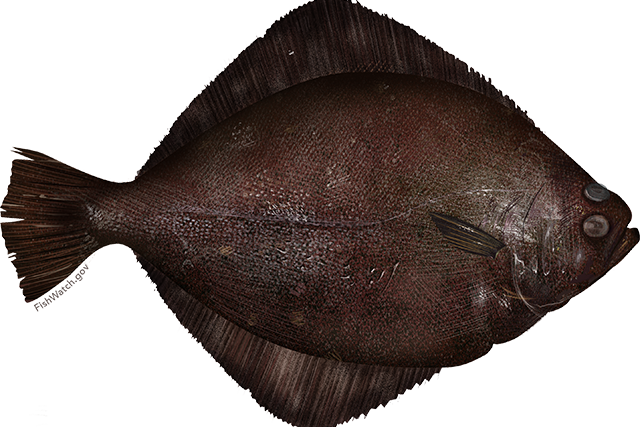
\includegraphics{petrale_sole}~\\[0.5cm]
%\pdftooltip{\includegraphics{Sebastes_alutus}}{This is a fish.}



Chantel R. Wetzel\textsuperscript{1}\\


\vspace{.5cm}

\small
\textsuperscript{1}Northwest Fisheries Science Center, U.S. Department of Commerce, National Oceanic and Atmospheric Administration, National Marine Fisheries Service, 2725 Montlake Boulevard East, Seattle, Washington 98112\\

\vspace{.3cm}





\vspace{1cm}

\vfill
June 2019


\vspace{.3cm}
%Bottom of the page
%{\large \today}

\newpage

\vspace{3cm}

Please cite as:\\

Wetzel, C.R. 2019. Status of petrale sole (\textit{Eopsetta jordani}) along the U.S. west coast in 2018. Pacific Fishery Management Council, 7700 Ambassador Place NE, Suite 200, Portland, OR 97220. 

\vspace{3cm}

\maketitle






\pagenumbering{roman}
\setcounter{page}{1}
\end{center}

{
\setcounter{tocdepth}{4}
\tableofcontents
}
\setlength{\parskip}{5mm plus1mm minus1mm} \pagebreak

\setcounter{page}{1} \renewcommand{\thefigure}{\alph{figure}}
\renewcommand{\thetable}{\alph{table}}

\section*{Executive Summary}\label{executive-summary}
\addcontentsline{toc}{section}{Executive Summary}

\subsection*{Stock}\label{stock}
\addcontentsline{toc}{subsection}{Stock}

This assessment reports the status of the petrale sole
(\emph{Eopsetta jordani}) off U.S. coast of California, Oregon, and
Washington using data through 2018. While petrale sole are modeled as a
single stock, the spatial aspects of the coast-wide population are
addressed through geographic separation of data sources/fleets where
possible. There is currently no genetic evidence suggesting distinct
biological stocks of petrale sole off the U.S. coast. The limited
tagging data available to describe adult movement suggests that petrale
sole may have some homing ability for deep water spawning sites but also
have the ability to move long distances between spawning sites,
inter-spawning season, as well as seasonally.

\subsection*{Landings}\label{landings}
\addcontentsline{toc}{subsection}{Landings}

While records do not exist, the earliest catches of petrale sole are
reported in 1876 in California and 1884 in Oregon. In this assessment,
fishery removals have been divided among 4 fleets: 1) winter North
trawl, 2) summer North trawl, 3) winter South trawl, and 4) summer South
trawl. Landings for the North fleet are defined as fish landed in
Washington and Oregon ports. Landings for the South fleet are defined as
fish landed in California ports. Recent annual catches between 1981-2018
range between 755 and 3008 mt per year and the most recent year landing
are shown in Table \ref{tab:Exec_catch}. Petrale sole are caught nearly
exclusively by trawl fleets; non-trawl gears contribute less than 3\% of
the catches. Based on the 2005 assessment, annual catch limits (ACLs)
were reduced to 2499 mt for 2007-2008. Following the 2009 assessment
ACLs were further reduced to a low of 976 mt for 2011 and have
subsequently increased to a high value of 3,136 for 2017. From the
inception of the fishery through the war years, the vast majority of
catches occurred between March and October (the summer fishery), when
the stock is dispersed over the continental shelf. The post-World War II
period witnessed a steady decline in the amount and proportion of annual
catches occurring during the summer months (March-October). Conversely,
petrale sole catch during the winter season (November-February), when
the fishery targets spawning aggregations, has exhibited a steadily
increasing trend since the 1940s. From the mid-1980s through the early
2000s, catches during the winter months were roughly equivalent to or
exceeded catches throughout the remainder of the year, whereas during
the past 10 years the relative catches during the winter and summer have
been more variable across years (\ref{tab:Exec_catch}). petrale sole are
a desirable market species and discarding has historically been low.

\begin{table}[ht]
\centering
\caption{Landings (mt) for the past 10 years for petrale sole by source.} 
\label{tab:Exec_catch}
\begin{tabular}{l>{\centering}p{0.7in}>{\centering}p{0.7in}>{\centering}p{0.7in}>{\centering}p{0.7in}>{\centering}p{0.7in}}
  \hline
Year & Winter (N) & Summer (N) & Winter (S) & Summer (S) & Total Landings \\ 
  \hline
2009 & 846.71 & 641.75 & 469.66 & 250.38 & 2208.49 \\ 
  2010 & 258.09 & 292.34 & 77.60 & 120.95 & 748.98 \\ 
  2011 & 221.60 & 423.11 & 39.59 & 77.70 & 762.00 \\ 
  2012 & 406.05 & 477.71 & 124.46 & 107.63 & 1115.85 \\ 
  2013 & 509.04 & 1007.26 & 130.10 & 278.35 & 1924.74 \\ 
  2014 & 852.90 & 860.31 & 273.40 & 354.19 & 2340.80 \\ 
   \hline
\end{tabular}
\end{table}

\FloatBarrier

\begin{figure}
\centering
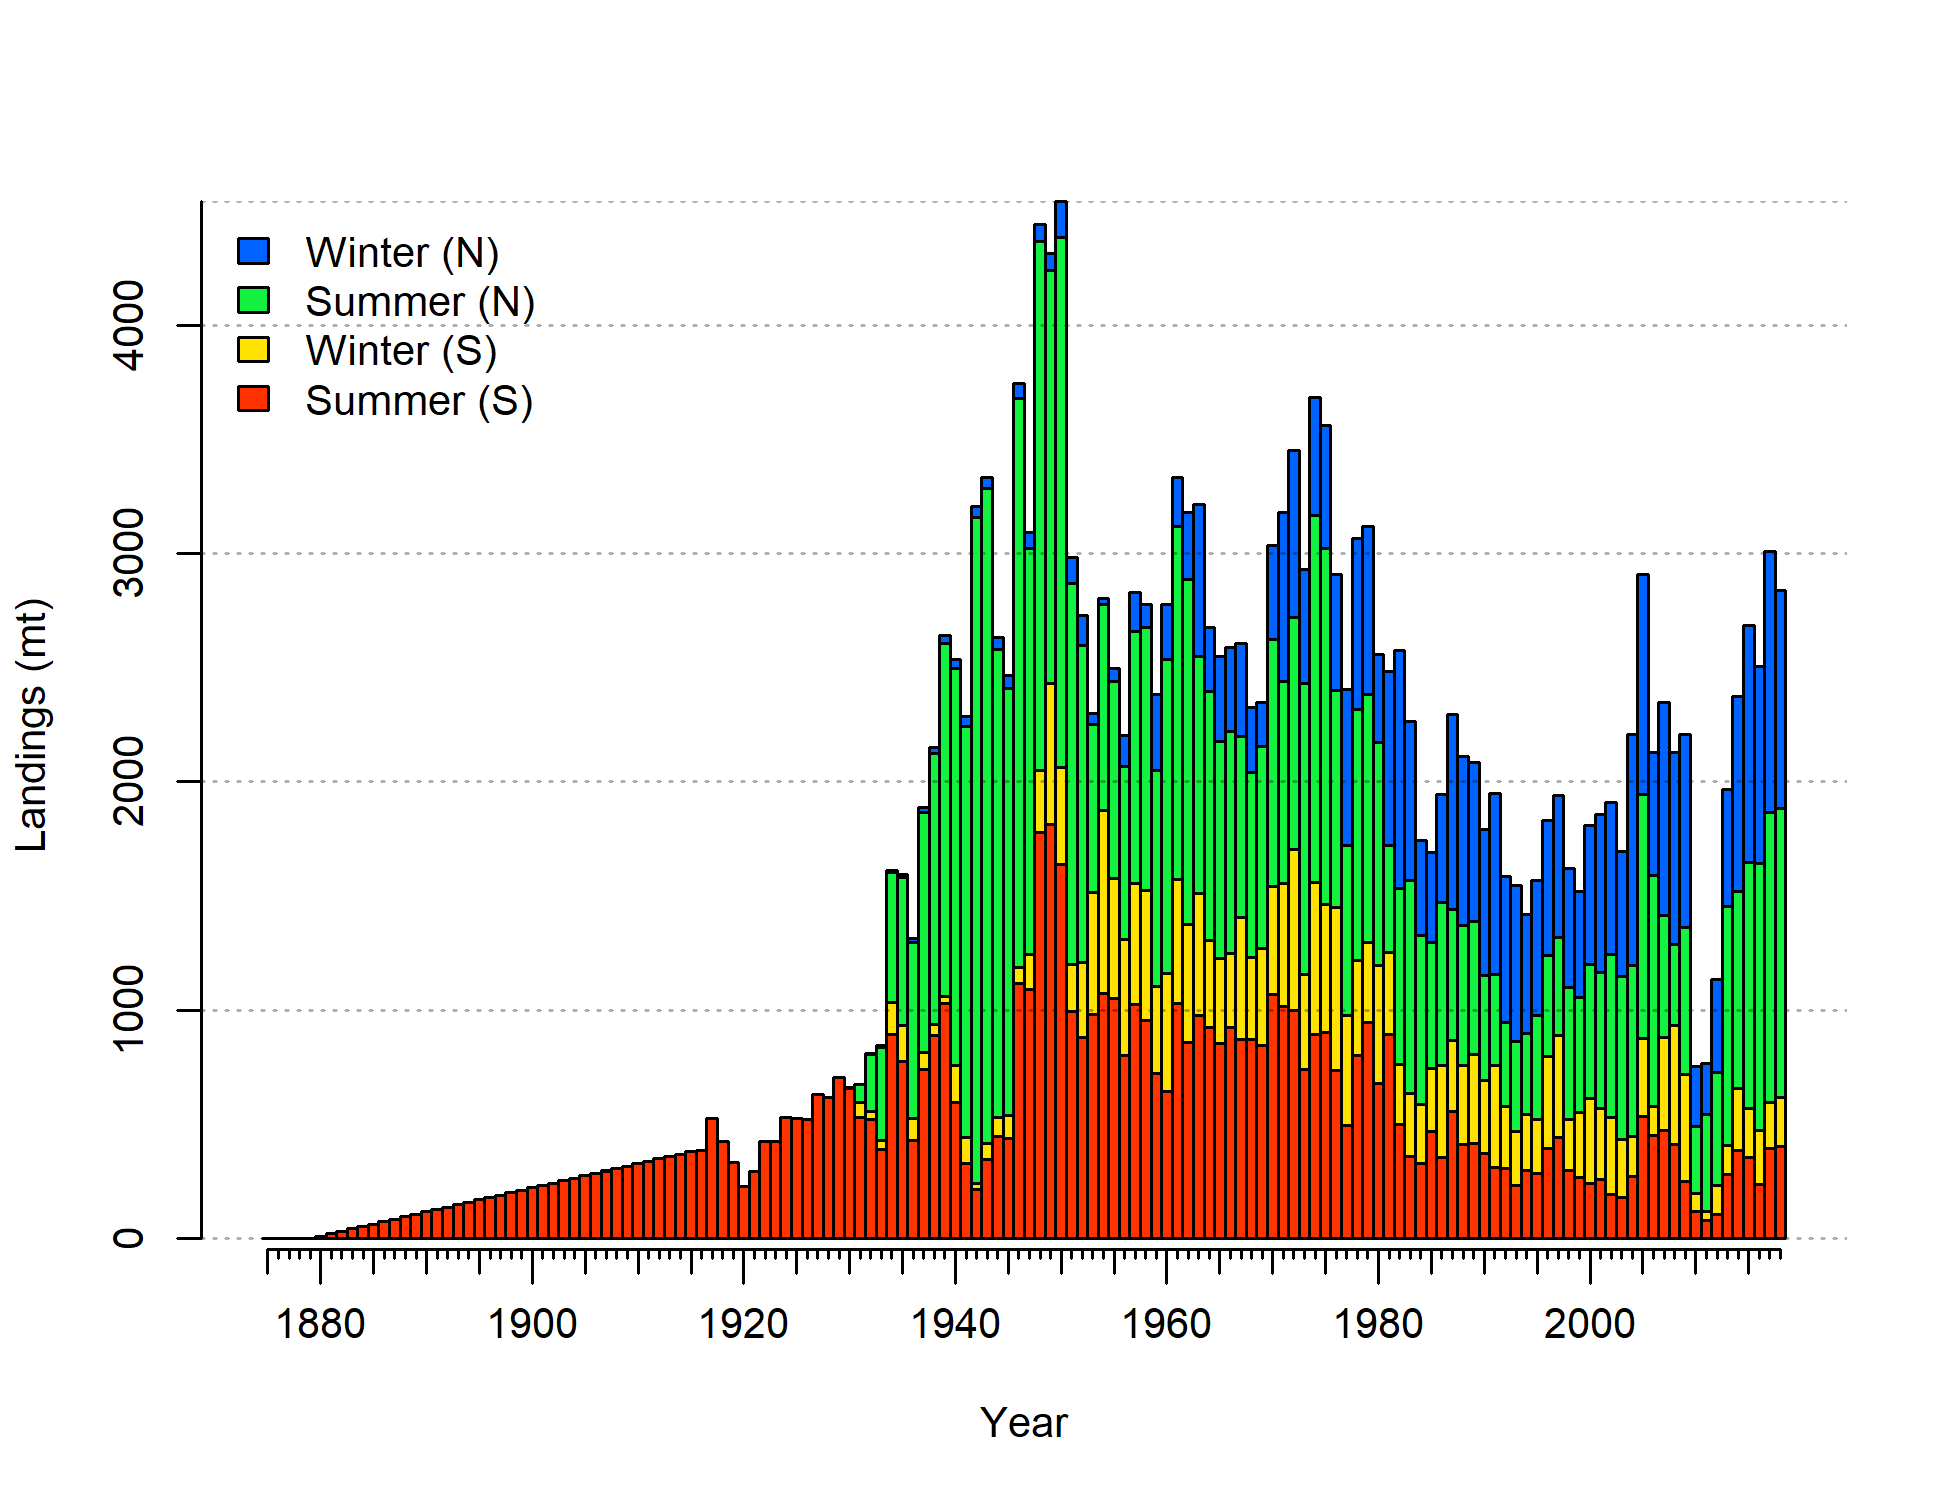
\includegraphics{r4ss/plots_mod1/catch2 landings stacked.png}
\caption{'Landings of by the Northern and Southern winter and summer
fleets of the US west coast. \label{fig:Exec_catch1}}
\end{figure}

\FloatBarrier

\subsection*{Data and Assessment}\label{data-and-assessment}
\addcontentsline{toc}{subsection}{Data and Assessment}

This an update assessment for petrale sole, which was last assessed in
2013 and updated in 2015. The update assessment was conducted using the
length- and age-structured modeling software Stock Synthesis (version
3.30.13). The coastwide population was modeled allowing separate growth
and mortality parameters for each sex (a two-sex model) with the fishing
year beginning on November 1 and ending on October 31. The fisheries are
structured seasonally based on winter (November to February) and summer
(March to October) fishing seasons due to the development and growth of
the wintertime fishery, which began in the 1950s. In recent decades
wintertime catches have often exceed summertime catches. The fisheries
modeled as the North Winter and North Summer, where the north includes
both Washington and Oregon, and South Winter and South Summer
encompasses California fisheries.

The model includes catch, length- and age-frequency data from the trawl
fleets as well as standardized winter fishery catch-per-unit-effort
(CPUE) indices. Biological data are derived from both port and on-board
observer sampling programs. The National Marine Fisheries Service (NMFS)
AFSC/NWFSC West Coast Triennial Shelf Survey early (1980, 1983, 1986,
1989, 1992) and late period (1995, 1998, 2001, and 2004) and the NWFSC
West Coast Groundfish Bottom Trawl Survey (2003-2018) relative biomass
indices and biological sampling provide fishery independent information
on relative trend and demographics of the petrale sole stock.

\subsection*{Updated Data}\label{updated-data}
\addcontentsline{toc}{subsection}{Updated Data}

The base stock assessment model structure is consistent with the 2013
assessment and the 2015 update, except as noted here. Modifications from
the previous assessment model include:

\begin{enumerate}

\item Model fitting using latest version of Stock Synthesis (SS v.3.30.13). 

\item Added commercial fishery catch data (2015-2018).

\item Updated historical composition data from the commercial fishery (length and age data) and new data (2015 - 2018) expanded to trip and catch based on current best practices.

\item Updated discard rate, average weight, and discard length composition data (2014-2017).

\item NWFSC West Coast Groundfish Bottom Trawl Survey index of abundance was calculated using VAST.

\item Updated NWFSC West Coast Groundfish Bottom Trawl Survey length and age data (2015-2018) with all years data expanded to the tow and strata.

\item AFSC/NWFSC West Coast Triennial Shelf Survey early and late index of abundance were calculated using VAST.

\item Model tuning to re-weight data. 

\item Length-weight relationship parameters estimated outside of the stock assessment model from the NWFSC West Coast Groundfish Bottom Trawl Survey data up to 2018 and input as fixed values.

\item Update the natural mortality prior for female and male fish.

\end{enumerate}

\subsection*{Stock Biomass}\label{stock-biomass}
\addcontentsline{toc}{subsection}{Stock Biomass}

Petrale sole were lightly exploited during the early 1900s, but by the
1950s the fishery was well developed and showing clear signs of
depletion and declines in catches and biomass (Figures
\ref{fig:Exec_catch1} and \ref{fig:Spawnbio_all}). The rate of decline
in spawning biomass accelerated through the 1930s-1970s reaching
minimums generally around or below 10\% of the unexploited levels during
the 1980s through the early 2000s (Figure \ref{fig:RelDeplete_all}). The
petrale sole spawning stock biomass is estimated to have increased in
recent year due to reduced catches during rebuilding and in response to
above average recruitment in 2006, 2007, and 2008. The 2019 estimated
spawning biomass relative to unfished equilibrium spawning biomass is
above the target of 25\% of unfished spawning biomass at 32.3\%
(\(\sim\) 95\% asymptotic interval: \(\pm\) 21.9\%-42.6\%).

\begin{figure}
\centering
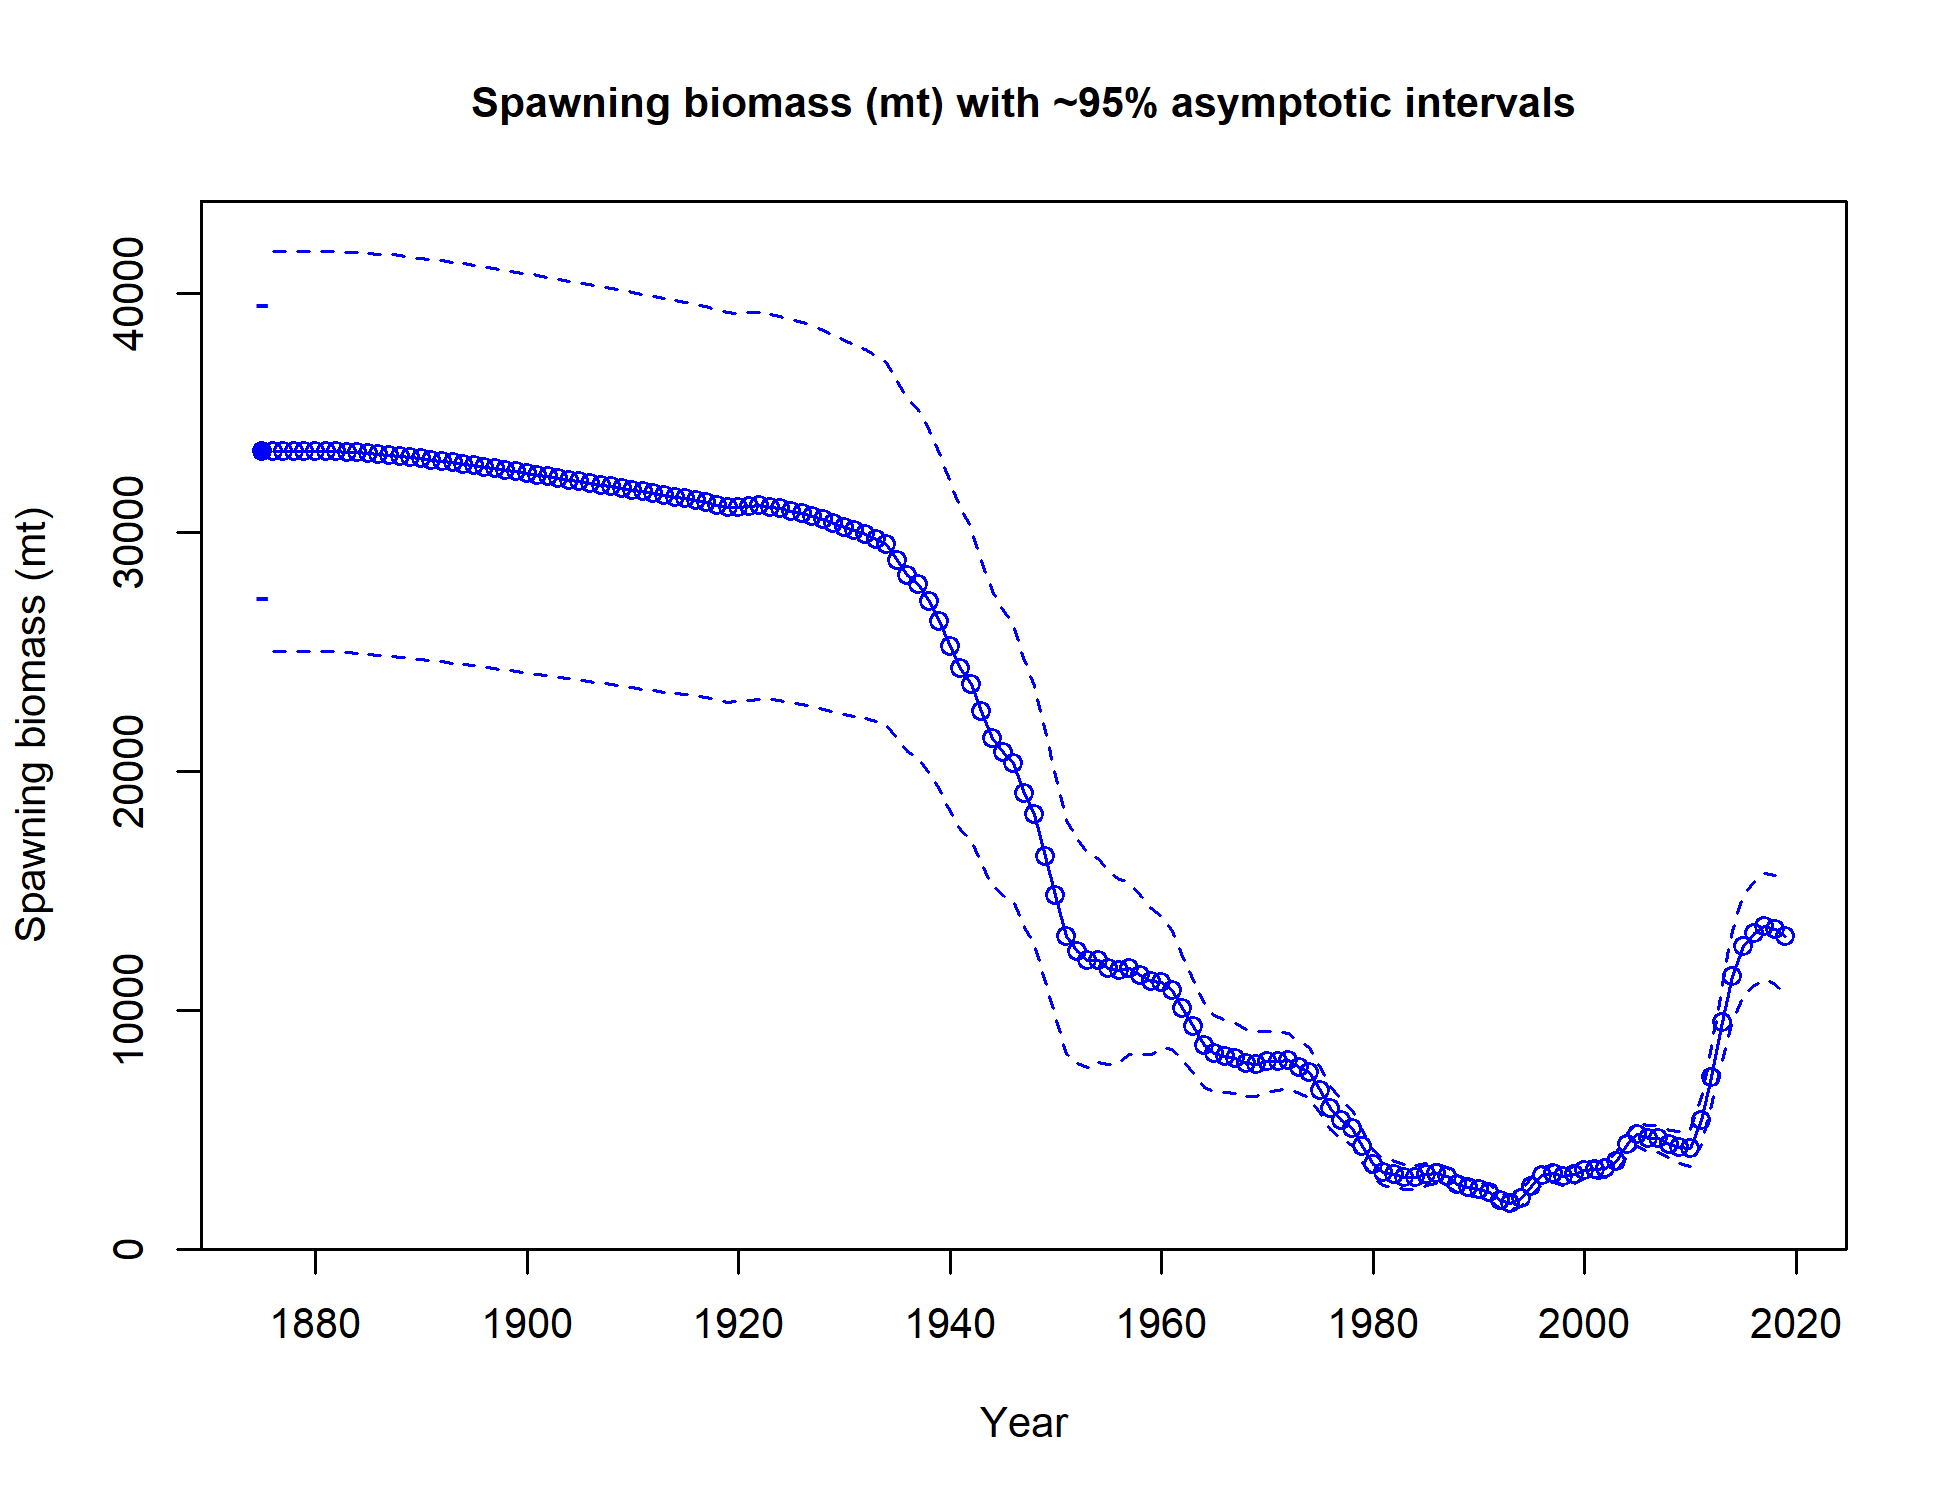
\includegraphics{r4ss/plots_mod1/ts7_Spawning_biomass_(mt)_with_95_asymptotic_intervals_intervals.png}
\caption{Estimated time-series of spawning biomass trajectory (circles
and line: median; light broken lines: 95\% credibility intervals) for
the base assessment model. \label{fig:Spawnbio_all}}
\end{figure}

\begin{figure}
\centering
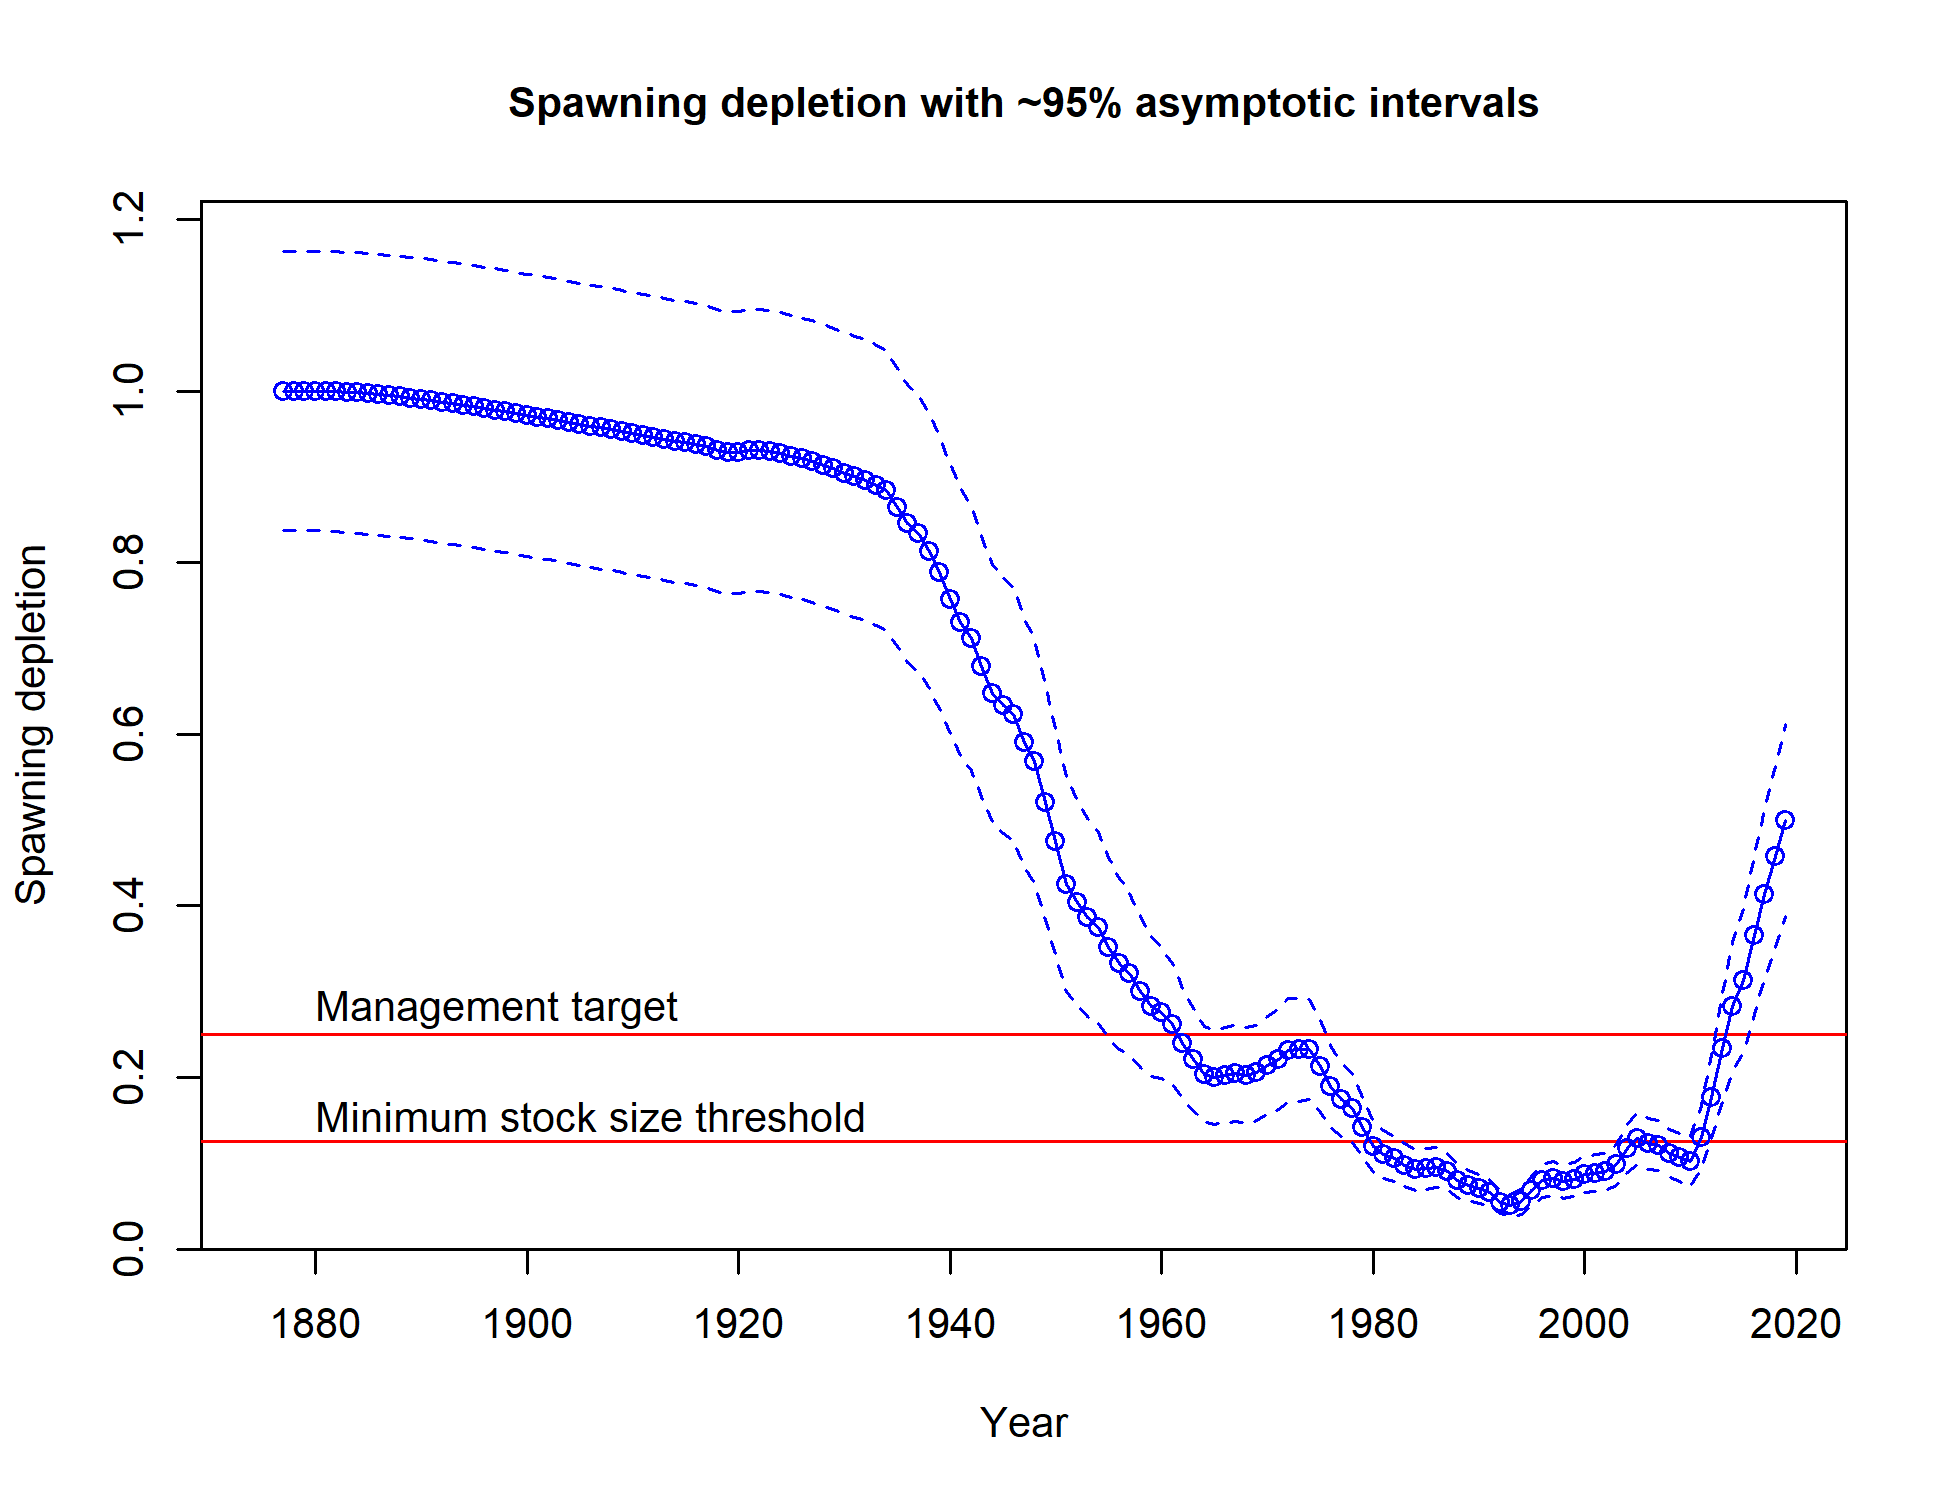
\includegraphics{r4ss/plots_mod1/ts9_Spawning_depletion_with_95_asymptotic_intervals_intervals.png}
\caption{Estimated time-series of relative spawning biomass (depletion)
(circles and line: median; light broken lines: 95\% credibility
intervals) for the base assessment model. \label{fig:RelDeplete_all}}
\end{figure}

\begin{table}[ht]
\centering
\caption{Recent trend in estimated spawning biomass (mt) and estimated relative spawning biomass (depletion).} 
\label{tab:SpawningDeplete_mod1}
\begin{tabular}{l>{\centering}p{1.3in}>{\centering}p{1.2in}>{\centering}p{1in}>{\centering}p{1.2in}}
  \hline
Year & Spawning Biomass (mt) & \~{} 95\% Confidence Interval & Estimated Relative Spawning Biomass & \~{} 95\% Confidence Interval \\ 
  \hline
2010 & 3494 & 2845 - 4143 & 0.114 & 0.077 - 0.152 \\ 
  2011 & 4414 & 3606 - 5222 & 0.144 & 0.098 - 0.191 \\ 
  2012 & 5904 & 4858 - 6950 & 0.193 & 0.132 - 0.255 \\ 
  2013 & 7751 & 6410 - 9091 & 0.254 & 0.174 - 0.333 \\ 
  2014 & 9284 & 7682 - 10886 & 0.304 & 0.209 - 0.398 \\ 
  2015 & 10202 & 8441 - 11962 & 0.334 & 0.231 - 0.436 \\ 
  2016 & 10439 & 8593 - 12284 & 0.342 & 0.237 - 0.446 \\ 
  2017 & 10531 & 8606 - 12457 & 0.345 & 0.240 - 0.449 \\ 
  2018 & 10213 & 8186 - 12240 & 0.334 & 0.231 - 0.437 \\ 
  2019 & 9867 & 7682 - 12052 & 0.323 & 0.219 - 0.426 \\ 
   \hline
\end{tabular}
\end{table}

\FloatBarrier

\subsection*{Recruitment}\label{recruitment}
\addcontentsline{toc}{subsection}{Recruitment}

Annual recruitment was treated as stochastic, and estimated as annual
deviations from log-mean recruitment where mean recruitment is the
fitted Beverton-Holt stock recruitment curve. The time-series of
estimated recruitments shows a relationship with the decline in spawning
biomass, punctuated by larger recruitments (Figure
\ref{fig:Recruits_all}) in 2006, 2007, and 2008. The five largest
estimated recruitment estimated with the model (in ascending order)
occurred in 2006, 2007, 1998, 1966, and 2008. The four lowest
recruitments estimated within the model (in ascending order) occurred in
1986, 1992, 1973, and 1987.

\begin{figure}
\centering
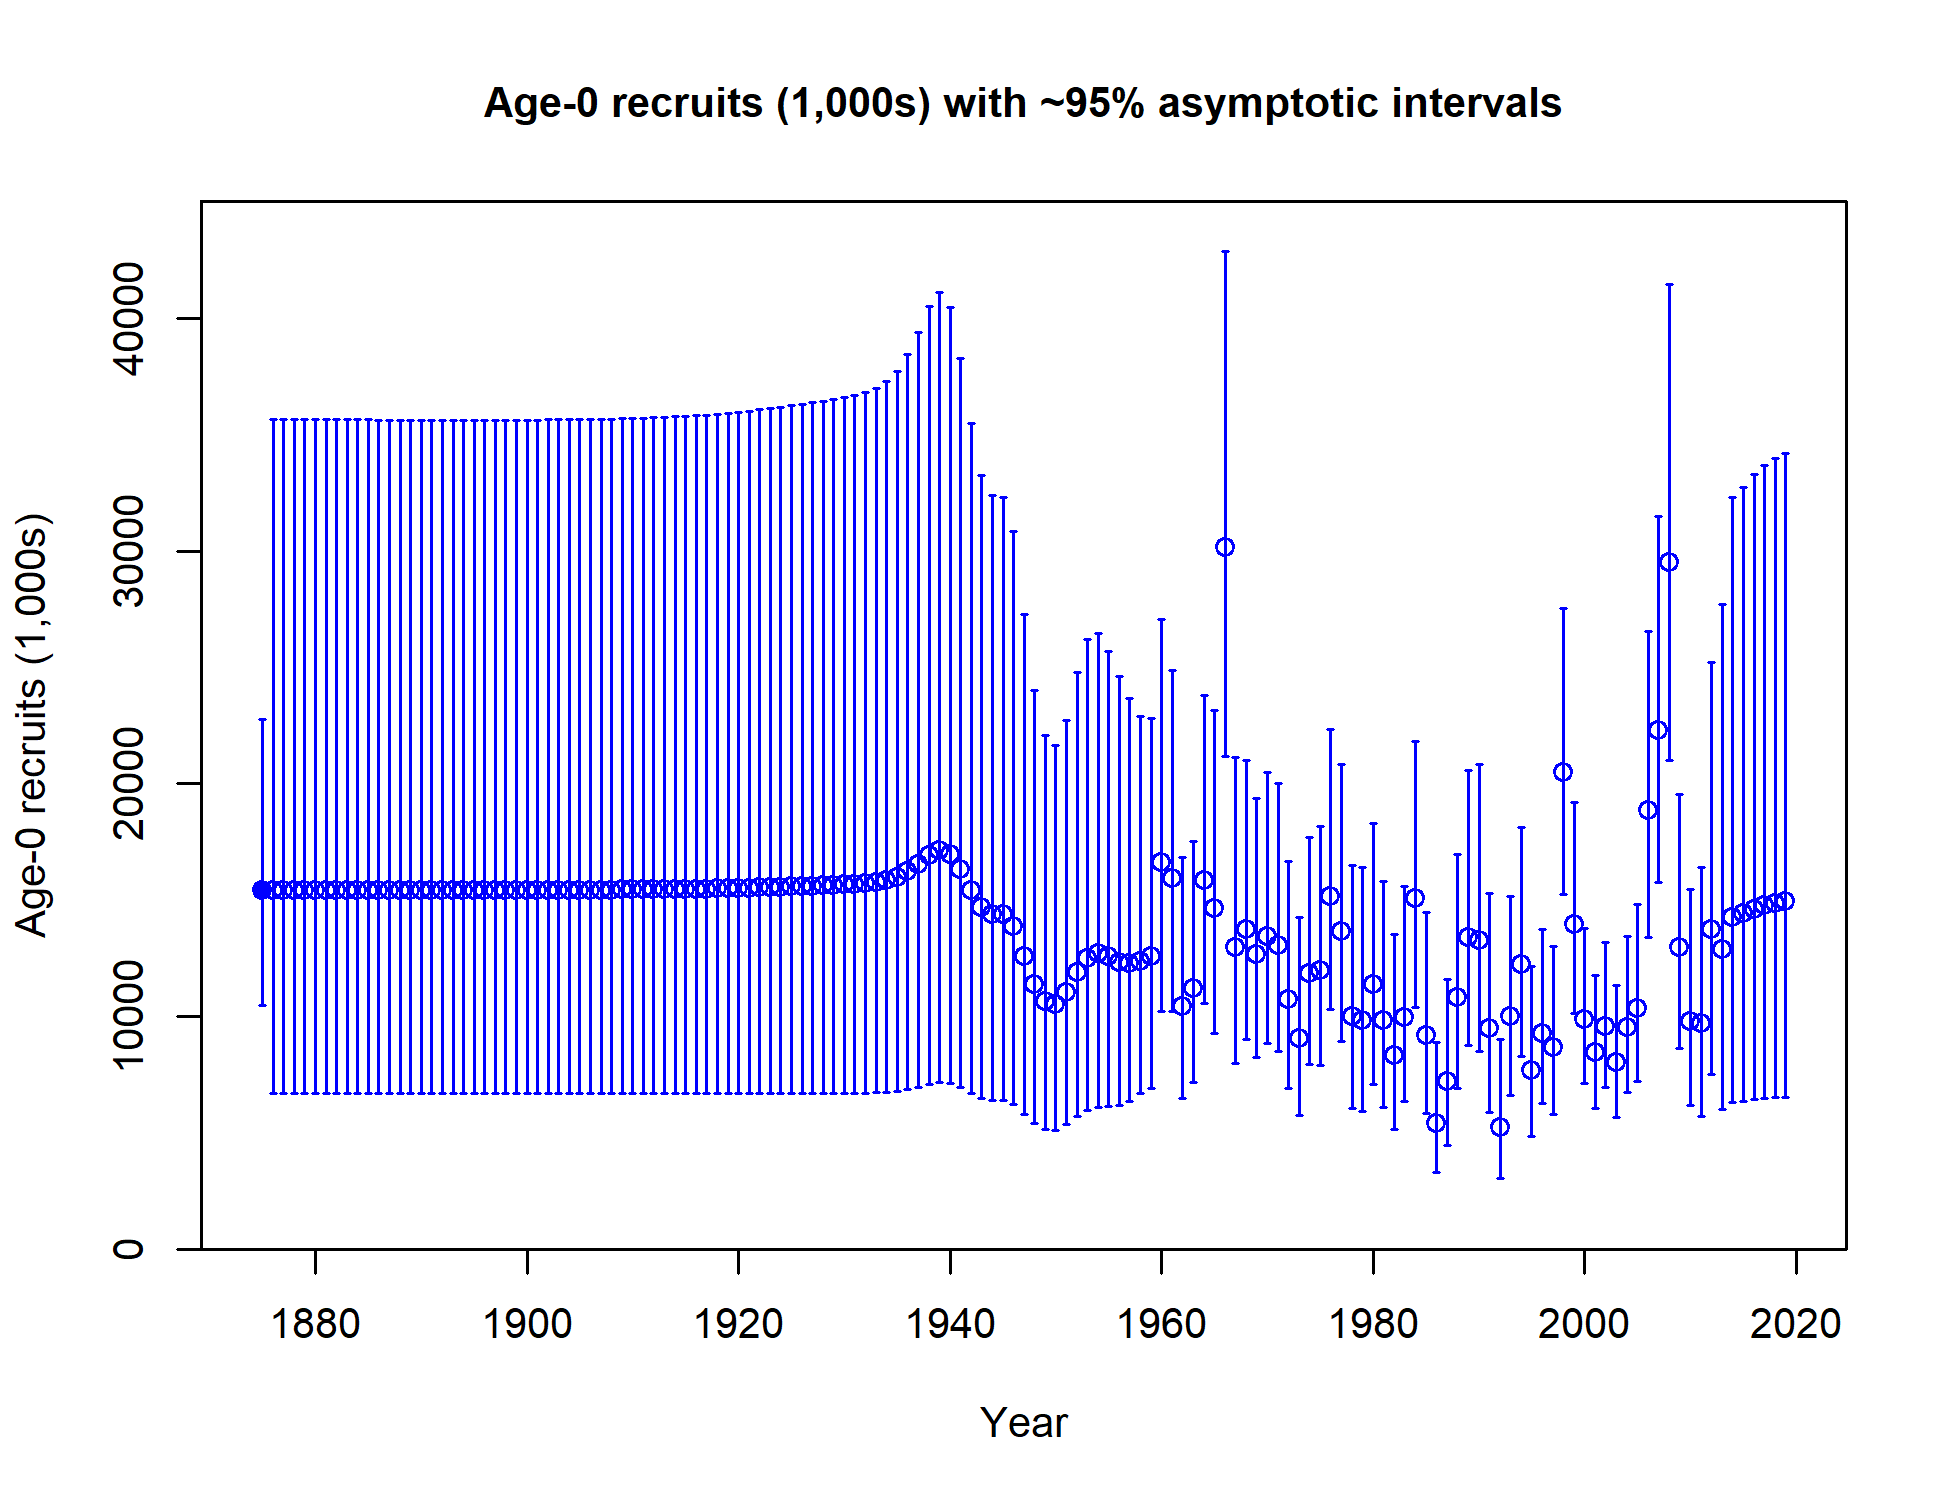
\includegraphics{r4ss/plots_mod1/ts11_Age-0_recruits_(1000s)_with_95_asymptotic_intervals.png}
\caption{Time-series of estimated petrale sole recruitments for the base
model with 95\% confidence or credibility intervals.
\label{fig:Recruits_all}}
\end{figure}

\begin{table}[ht]
\centering
\caption{Recent estimated trend in recruitment and estimated recruitment deviations determined from the base model. The recruitment deviations for 2018 and 2019 were fixed at zero within the model.} 
\label{tab:Recruit_mod1}
\begin{tabular}{>{\centering}p{.8in}>{\centering}p{1.0in}>{\centering}p{1.4in}>{\centering}p{1.0in}>{\centering}p{1.4in}}
  \hline
Year & Estimated Recruitment & \~{} 95\% Confidence Interval & Estimated Recruitment Devs. & \~{} 95\% Confidence Interval \\ 
  \hline
2010 & 11740 & 7281 - 18929 & -0.083 & -0.411 - 0.244 \\ 
  2011 & 13434 & 8205 - 21994 & -0.014 & -0.358 - 0.330 \\ 
  2012 & 19781 & 12473 - 31372 & 0.306 & 0.002 - 0.609 \\ 
  2013 & 12763 & 7331 - 22221 & -0.183 & -0.631 - 0.265 \\ 
  2014 & 13826 & 7883 - 24251 & -0.130 & -0.586 - 0.325 \\ 
  2015 & 13751 & 7464 - 25334 & -0.149 & -0.664 - 0.366 \\ 
  2016 & 13924 & 6927 - 27992 & -0.160 & -0.771 - 0.451 \\ 
  2017 & 15071 & 6851 - 33154 & -0.104 & -0.837 - 0.630 \\ 
  2018 & 17012 & 7437 - 38914 & 0.000 & -0.784 - 0.784 \\ 
  2019 & 16935 & 7409 - 38710 & 0.000 & -0.784 - 0.784 \\ 
   \hline
\end{tabular}
\end{table}

\FloatBarrier

\subsection*{Exploitation Status}\label{exploitation-status}
\addcontentsline{toc}{subsection}{Exploitation Status}

The relative spawning biomass of of petrale sole was estimated to have
dropped below the management target (25\%) for the first time in 1976.
The stock continued to decline and first fell below the minimum stock
size threshold level of 12.5\% in 1982. The relative spawning biomass
remained around the threshold stock size until approximately 2010, with
the stock reaching its lowest relative spawning biomass level in 1993 at
5.8\%. In 2009 petrale sole was formally declared overfished. Fishing
mortality rates sharply declined during the rebuilding period relative
to previous year rates which exceeded the target (Figure
\ref{fig:SPR_all}). After reduced harvests, the 2015 update stock
assessment estimated the stock to have rebuilt to the management target
(25\%) in 2014. This update estimates that the relative spawning biomass
exceed 25\% in 2013 with harvest rates in the most recent years
remaining just under of the target rate (Figure \ref{fig:SPR_all}).

\begin{table}[ht]
\centering
\caption{Recent trend in spawning potential ratio 1-SPR and summary exploitation rate for age 3+ biomass for petrale sole.} 
\label{tab:SPR_Exploit_mod1}
\begin{tabular}{l>{\centering}p{0.9in}>{\centering}p{1.2in}>{\centering}p{1.2in}>{\centering}p{1.2in}}
  \hline
Year & 1-SPR & \~{} 95\% Confidence Interval & Exploitation Rate & \~{} 95\% Confidence Interval \\ 
  \hline
2009 & 0.822 & 0.757 - 0.888 & 0.271 & 0.223 - 0.318 \\ 
  2010 & 0.625 & 0.521 - 0.728 & 0.091 & 0.072 - 0.111 \\ 
  2011 & 0.552 & 0.446 - 0.658 & 0.062 & 0.049 - 0.075 \\ 
  2012 & 0.568 & 0.466 - 0.671 & 0.074 & 0.060 - 0.089 \\ 
  2013 & 0.632 & 0.535 - 0.730 & 0.111 & 0.090 - 0.131 \\ 
  2014 & 0.633 & 0.537 - 0.729 & 0.126 & 0.104 - 0.149 \\ 
  2015 & 0.644 & 0.549 - 0.738 & 0.138 & 0.113 - 0.163 \\ 
  2016 & 0.618 & 0.521 - 0.714 & 0.129 & 0.105 - 0.153 \\ 
  2017 & 0.654 & 0.561 - 0.747 & 0.155 & 0.126 - 0.185 \\ 
  2018 & 0.649 & 0.555 - 0.743 & 0.152 & 0.121 - 0.183 \\ 
   \hline
\end{tabular}
\end{table}

\FloatBarrier

\begin{figure}
\centering
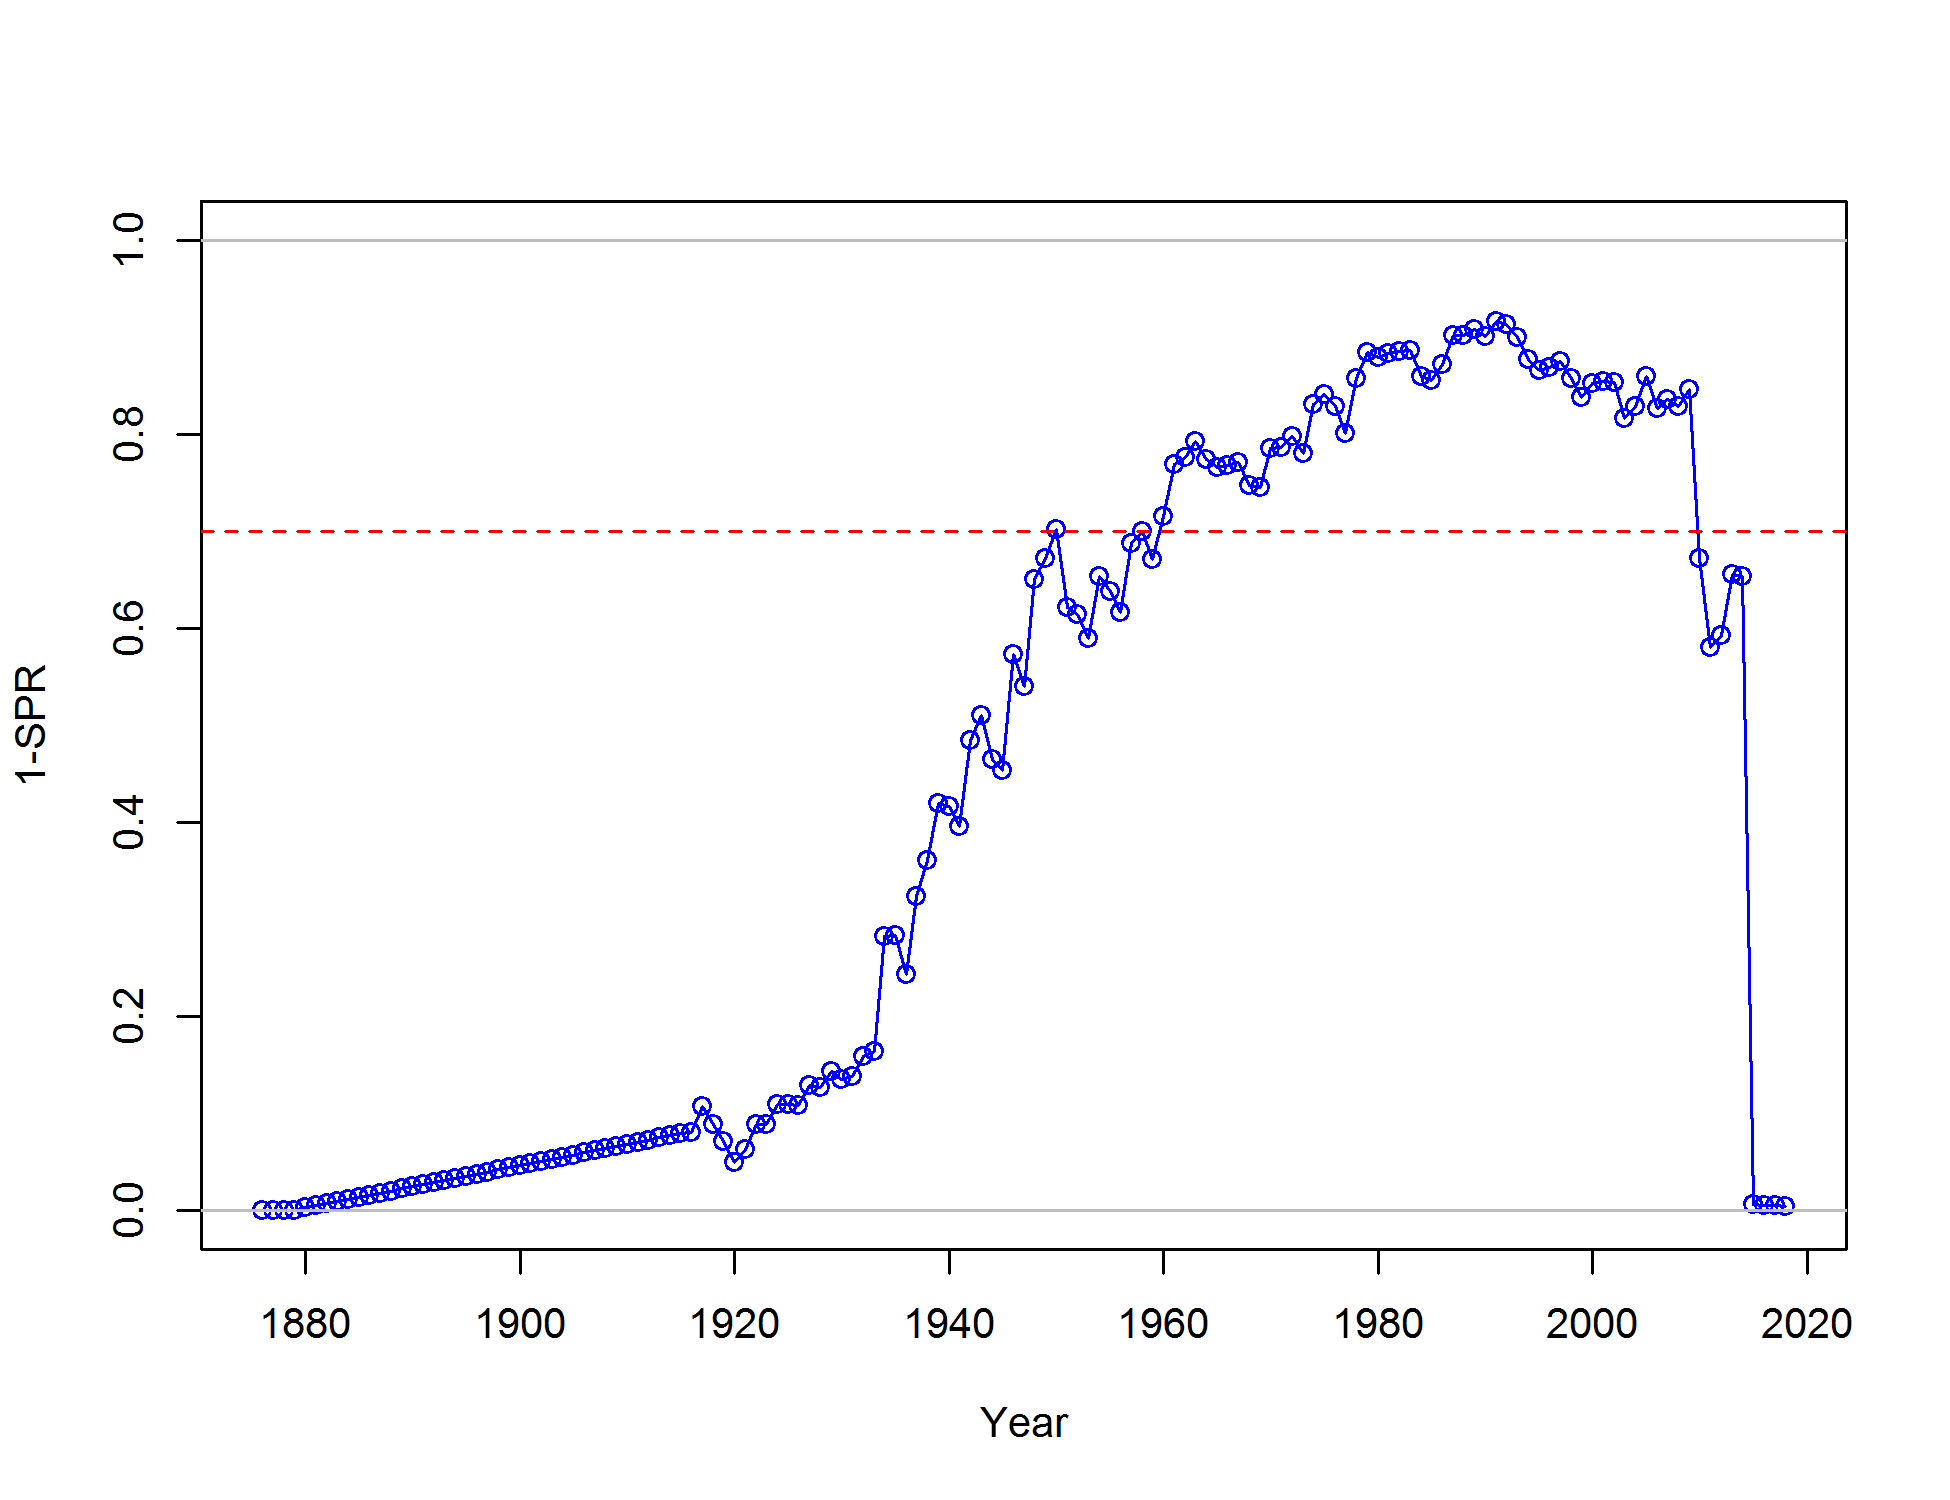
\includegraphics{r4ss/plots_mod1/SPR2_minusSPRseries.png}
\caption{Estimated relative spawning potential ratio 1-SPR for the base
model. One minus SPR is plotted so that higher exploitation rates occur
on the upper portion of the y-axis. The management target is plotted as
a red horizontal line and values above this reflect harvests in excess
of the overfishing proxy based on the SPR30\% harvest rate. The last
year in the time-series is 2018. \label{fig:SPR_all}}
\end{figure}

\begin{figure}
\centering
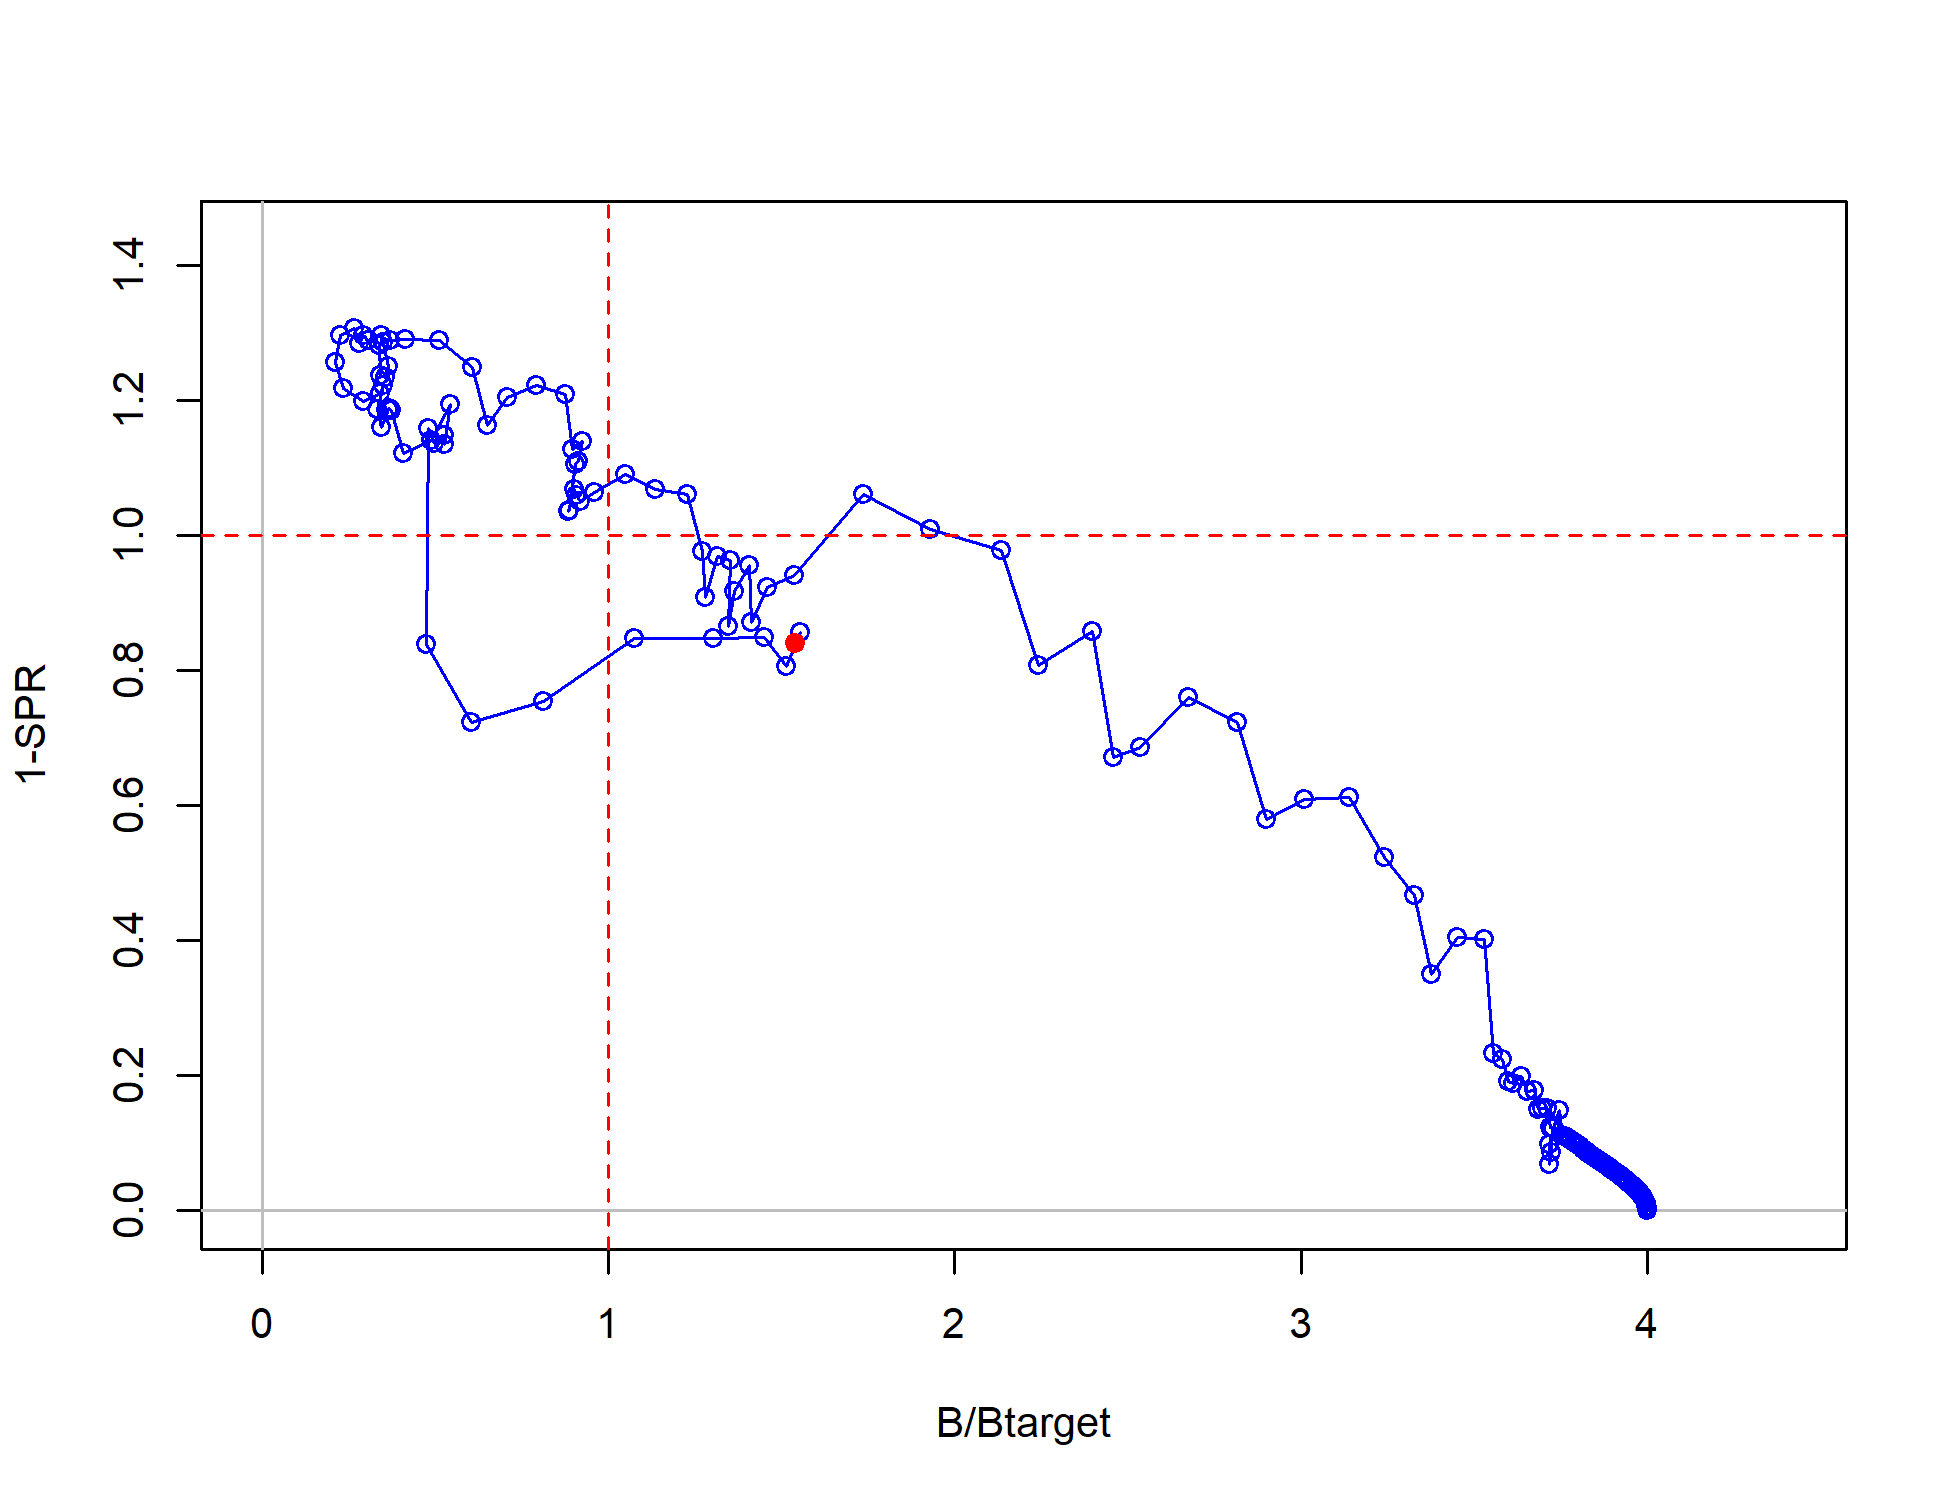
\includegraphics{r4ss/plots_mod1/SPR4_phase.png}
\caption{Phase plot of estimated 1-SPR(\%) vs.~relative spawning biomass
(B/Btarget) for the base case model. The red circle indicates 2018
estimated status and exploitation for petrale sole.
\label{fig:Phase_all}}
\end{figure}

\FloatBarrier

\subsection*{Ecosystem Considerations}\label{ecosystem-considerations}
\addcontentsline{toc}{subsection}{Ecosystem Considerations}

Ecosystem factors have not been explicitly modeled in this assessment,
but there are several aspects of the California current ecosystem that
may impact petrale sole population dynamics and warrant further
research. Castillo
(\protect\hyperlink{ref-castillo_g.c._fluctuations_1992}{1992}) and
Castillo et al.
(\protect\hyperlink{ref-castillo_latitudinal_1995}{1995}) suggest that
density-independent survival of early life stages is low and show that
offshore Ekman transportation of eggs and larvae may be an important
source of variation in year-class strength in the Columbia INPFC area.
The effects of the Pacific Decadal Oscillation on California current
temperature and productivity (Mantua et al.
\protect\hyperlink{ref-mantua_pacific_1997}{1997}) may also contribute
to non-stationary recruitment dynamics for petrale sole. The prevalence
of a strong late 1990s year-class for many West Coast groundfish species
suggests that environmentally driven recruitment variation may be
correlated among species with relatively diverse life history
strategies. Although current research efforts along these lines are
limited, a more explicit exploration of ecosystem processes may be
possible in future petrale sole stock assessments if resources are
available for such investigations.

\subsection*{Reference Points}\label{reference-points}
\addcontentsline{toc}{subsection}{Reference Points}

This stock assessment estimates that the spawning biomass of petrale
sole is above the management target. Due to reduced landings and the
large 2008 year-class, an increasing trend in spawning biomass was
estimated in the base model. The estimated depletion in 2019 is 32.3\%
(\(\sim\) 95\% asymptotic interval: \(\pm\) 21.9\%-42.6\%),
corresponding to an spawning biomass of 9,867 mt (\(\sim\) 95\%
asymptotic interval: 7,682-12,052 mt). Unfished age 3+ biomass was
estimated to be 49,439.6 mt in the base model. The target spawning
biomass based on the biomass target (\(SB_{25\%}\)) is 7,638.7 mt, with
an equilibrium catch of 2,830.3 mt. Equilibrium yield at the proxy
\(F_{MSY}\) harvest rate corresponding to \(SPR_{30\%}\) is 2,819.8 mt.
Estimated MSY catch is at a 2,835.9 spawning biomass of 7,005.9 mt
(22.9\% relative spawning biomass).

\begin{table}[ht]
\centering
\caption{Summary of reference 
                                      points and management quantities for the 
                                      base case.} 
\label{tab:Ref_pts_mod1}
\begin{tabular}{>{\raggedright}p{4.1in}>{\centering}p{.65in}>{\centering}p{.65in}>{\centering}p{.65in}}
  \hline
\textbf{Quantity} & \textbf{Estimate} & \textbf{$\sim$2.5\%  Confidence Interval} & \textbf{$\sim$97.5\%  Confidence Interval} \\ 
  \hline
Unfished spawning biomass (mt) & 30554.7 & 24634.6 & 36474.8 \\ 
  Unfished age 3+ biomass (mt) & 49439.6 & 41597 & 57282.2 \\ 
  Unfished recruitment (R0, thousands) & 18626.7 & 11147.4 & 26106 \\ 
  Spawning biomass(2019 mt) & 9867.3 & 7682.4 & 12052.2 \\ 
  Relative spawning biomass (depletion) (2019) & 0.323 & 0.219 & 0.426 \\ 
  \textbf{$\text{Reference points based on } \mathbf{SB_{25\%}}$} &  &  &  \\ 
  Proxy spawning biomass ($B_{25\%}$) & 7638.7 & 6158.7 & 9118.7 \\ 
  SPR resulting in $B_{25\%}$ ($SPR_{B25\%}$) & 0.286 & 0.258 & 0.313 \\ 
  Exploitation rate resulting in $B_{25\%}$ & 0.182 & 0.163 & 0.2 \\ 
  Yield with $SPR_{B25\%}$ at $B_{25\%}$ (mt) & 2830.3 & 2624.2 & 3036.4 \\ 
  \textbf{\textit{Reference points based on SPR proxy for MSY}} &  &  &  \\ 
  Spawning biomass & 8096.3 & 6199.3 & 9993.3 \\ 
  $SPR_{30\%}$ &  &  &  \\ 
  Exploitation rate corresponding to $SPR_{30\%}$ & 0.173 & 0.145 & 0.2 \\ 
  Yield with $SPR_{30\%}$ at $SB_{SPR}$ (mt) & 2819.8 & 2590.1 & 3049.5 \\ 
  \textbf{\textit{Reference points based on estimated MSY values}} &  &  &  \\ 
  Spawning biomass at $MSY$ ($SB_{MSY}$) & 7005.9 & 5242.2 & 8769.6 \\ 
  $SPR_{MSY}$ & 0.266 & 0.201 & 0.331 \\ 
  Exploitation rate at $MSY$ & 0.195 & 0.164 & 0.225 \\ 
  $MSY$ (mt)  & 2835.9 & 2641.9 & 3029.9 \\ 
   \hline
\end{tabular}
\end{table}

\FloatBarrier

\subsection*{Management Performance}\label{management-performance}
\addcontentsline{toc}{subsection}{Management Performance}

The 2009 stock assessment estimated petrale sole to be at 11.6\% of
unfished spawning stock biomass in 2010. Based on the 2009 stock
assessment, the 2010 coast-wide ACL was reduced to 1,200 mt to reflect
the overfished status of the stock and the 2011 coast-wide overfishing
limit (OFL) and ACL were set at 1,021 mt and 976 mt, respectively (Table
\ref{tab:mnmgt_perform}).

Recent coast-wide annual landings have not exceeded the ACL. The 2009,
2011, and 2013 full assessments estimated that petrale sole have been
below the management target since the 1960s and below the overfished
threshold between the early 1980s and the early 2000s with fishing
mortality rates in excess of the current F-target for flatfish of
SPR30\%. The 2015 update assessment estimated that the stock had
recovered with the relative spawning biomass exceeding the management
target.

\begin{table}[ht]
\centering
\caption{Recent trend in total catch and  
                              landings (mt) relative to the management guidelines. 
                              Estimated total catch reflect the landings 
                              plus the model estimated discarded biomass based on discard rate data.} 
\label{tab:mnmgt_perform}
\scalebox{0.9}{
\begin{tabular}{>{\raggedleft}p{0.5in}>{\centering}p{1.1in}>{\centering}p{1.1in}>{\centering}p{1.1in}>{\centering}p{1.1in}}
  \hline
Year & OFL (mt; ABC prior to 2011) & ACL (mt; OY prior to 2011) & Total Landings (mt) & Estimated Total Catch (mt) \\ 
  \hline
\text{2009} & 2811 & 2433 & 2209 & 2329 \\ 
  \text{2010} & 2751 & 1200 & 755 & 867 \\ 
  \text{2011} & 1021 & 976 & 768 & 791 \\ 
  \text{2012} & 1275 & 1160 & 1135 & 1159 \\ 
  \text{2013} & 2711 & 2592 & 1936 & 1973 \\ 
  \text{2014} & 2774 & 2652 & 2373 & 2398 \\ 
  \text{2015} & 3073 & 2816 & 2686 & 2727 \\ 
  \text{2016} & 3208 & 2910 & 2506 & 2543 \\ 
  \text{2017} & 3208 & 3136 & 3008 & 3050 \\ 
  \text{2018} & 3152 & 3013 & 2840 & 2882 \\ 
   \hline
\end{tabular}
}
\end{table}

\FloatBarrier

\subsection*{Unresolved Problems and Major
Uncertainties}\label{unresolved-problems-and-major-uncertainties}
\addcontentsline{toc}{subsection}{Unresolved Problems and Major
Uncertainties}

Parameter uncertainty is explicitly captured in the asymptotic
confidence intervals reported throughout this assessment for key
parameters and management quantities. These intervals reflect the
uncertainty in the model fit to the data sources included in the
assessment, but do not include uncertainty associated with alternative
model configurations, weighting of data sources (a combination of input
sample sizes and relative weighting of likelihood components), or fixed
parameters.

There are a number of major uncertainties regarding model parameters
that have been explored via sensitivity analysis. The most notable
explorations involved the sensitivity of model estimates to:

\begin{enumerate}

\item Value of female natural mortality.

\item Sex ratio between female and male petrale sole.

\item Changes in estimated based on alternative data weighting approaches.

\end{enumerate}

Additionally, to date a reconstructed historical Washington catch
history has not been included in the petrale sole stock assessment.
Washington state is currently undergoing efforts to determine historical
catches.

\subsection*{Decision Table}\label{decision-table}
\addcontentsline{toc}{subsection}{Decision Table}

Model uncertainty has been described by the estimated uncertainty within
the base model and by the sensitivities to different model structure.

\begin{table}[ht]
\centering
\caption{Projections of potential OFL (mt) and ABC (mt) and the estimated spawning biomass and relative depletion based on ABC removals.  The 2019 and 2020 
                                               removals are set at the harvest limits currently set by management of XXX mt per year.} 
\label{tab:OFL_projection}
\begin{tabular}{>{\raggedleft}p{0.5in}>{\centering}p{1.1in}>{\centering}p{1.1in}>{\centering}p{1.6in}>{\centering}p{1.1in}}
  \hline
Year & OFL & ABC & Spawning Biomass (mt) & Relative Depletion \\ 
  \hline
2019 & 3436 & 3301 & 9867 & 0.323 \\ 
  2020 & 3189 & 3065 & 9191 & 0.301 \\ 
  2021 & 2987 & 2870 & 8630 & 0.282 \\ 
  2022 & 2843 & 2731 & 8235 & 0.270 \\ 
  2023 & 2764 & 2655 & 8035 & 0.263 \\ 
  2024 & 2742 & 2633 & 8009 & 0.262 \\ 
  2025 & 2757 & 2648 & 8087 & 0.265 \\ 
  2026 & 2790 & 2680 & 8201 & 0.268 \\ 
  2027 & 2824 & 2713 & 8304 & 0.272 \\ 
  2028 & 2851 & 2738 & 8379 & 0.274 \\ 
  2029 & 2869 & 2756 & 8427 & 0.276 \\ 
  2030 & 2880 & 2766 & 8455 & 0.277 \\ 
   \hline
\end{tabular}
\end{table}

\FloatBarrier

\begin{table}[ht]
\centering
\caption{Decision table summary of 10-year 
                                             projections beginning in 2021 
                                             for alternate states of nature based on 
                                             an axis of uncertainty for the base model. The removals in 2019 and 2020 were set at the defined management 
                                             specification of XXX mt for each year assuming full attainment.
                                             The range of natural mortality values corresponded to the 12.5 and 87.5th quantile
                                             from the uncertainty around final spawning biomass.
                                             Columns range over low, mid, and high
                                             states of nature, and rows range over different 
                                             assumptions of catch levels. The SPR30 catch stream is based on the equilibrium yield applying the SPR30 harvest rate.} 
\label{tab:Decision_table_mod1}
\scalebox{0.85}{
\begin{tabular}{l|cc|>{\centering}p{.7in}c|>{\centering}p{.7in}c|>{\centering}p{.7in}c}
   \multicolumn{3}{c}{}  &  \multicolumn{2}{c}{} 
                               & \multicolumn{2}{c}{\textbf{States of nature}} 
                               & \multicolumn{2}{c}{} \\
  \multicolumn{3}{c}{}  &  \multicolumn{2}{c}{Low State} 
                               & \multicolumn{2}{c}{Base} 
                               &  \multicolumn{2}{c}{High State} \\
 \hline
 & Year & Catch & Spawning Biomass & Depletion & Spawning Biomass & Depletion & Spawning Biomass & Depletion \\ 
  \hline
 & 2021 &  &  &  &  &  &  &  \\ 
   & 2022 &  &  &  &  &  &  &  \\ 
   & 2023 &  &  &  &  &  &  &  \\ 
  ABC & 2024 &  &  &  &  &  &  &  \\ 
   & 2025 &  &  &  &  &  &  &  \\ 
   & 2026 &  &  &  &  &  &  &  \\ 
   & 2027 &  &  &  &  &  &  &  \\ 
   & 2028 &  &  &  &  &  &  &  \\ 
   & 2029 &  &  &  &  &  &  &  \\ 
   & 2030 &  &  &  &  &  &  &  \\ 
   \hline
 & 2021 &  &  &  &  &  &  &  \\ 
   & 2022 &  &  &  &  &  &  &  \\ 
   & 2023 &  &  &  &  &  &  &  \\ 
  SPR  & 2024 &  &  &  &  &  &  &  \\ 
  target =  & 2025 &  &  &  &  &  &  &  \\ 
  0.34 & 2026 &  &  &  &  &  &  &  \\ 
   & 2027 &  &  &  &  &  &  &  \\ 
   & 2028 &  &  &  &  &  &  &  \\ 
   & 2029 &  &  &  &  &  &  &  \\ 
   & 2030 &  &  &  &  &  &  &  \\ 
   \hline
\end{tabular}
}
\end{table}

\FloatBarrier

\subsection*{Research and Data Needs}\label{research-and-data-needs}
\addcontentsline{toc}{subsection}{Research and Data Needs}

Progress on a number of research topics and data issues would
substantially improve the ability of this assessment to reliably and
precisely model petrale sole population dynamics in the future:

\begin{enumerate}

\item In the past many assessments have derived historical catches independently. The states of California and Oregon have completed comprehensive historical catch reconstructions. At the time of this assessment, a comprehensive historical catch reconstruction is not available for Washington. Completion of a Washington catch reconstruction would provide the best possible estimated catch series that accounts for all the catch and better resolves historical catch uncertainty for flatfish as a group.

\item Due to limited data, new studies on the maturity relationships for petrale sole would be beneficial.

\item Where possible, historical otolith samples aged using a combination of surface and break-and-burn methods should be re-aged using the break-and-burn method. Early surface read otoliths should also be re-aged using the break-and-burn method. Historical otoliths aged with a standard method will allow the further evaluation of the potential impacts of consistent under ageing using surface methods, changes in selectivity during early periods of time without any composition information, and potential changes in growth.

\item Studies on stock structure and movement of petrale sole, particularly with regard to the winter-summer spawning migration of petrale sole and the likely trans-boundary movement of petrale sole between U.S. and Canadian waters seasonally.

\item The extent of spatial variability on productivity processes such as growth, recruitment, and maturity is currently unknown and would benefit from further research.

\end{enumerate}

\begin{sidewaystable}[ht]
\centering
\caption{Base model results summary.} 
\label{tab:base_summary}
\scalebox{0.6}{
\begin{tabular}{r>{\centering}p{1.1in}>{\centering}p{1.1in}>{\centering}p{1.1in}>{\centering}p{1.1in}>{\centering}p{1.1in}>{\centering}p{1.1in}>{\centering}p{1.1in}>{\centering}p{1.1in}>{\centering}p{1.1in}>{\centering}p{1.1in}}
  \hline
Quantity & 2010 & 2011 & 2012 & 2013 & 2014 & 2015 & 2016 & 2017 & 2018 & 2019 \\ 
  \hline
OFL (mt) & 2751 & 1021 & 1275 & 2711 & 2774 & 3073 & 3208 & 3208 & 3152 &    1 \\ 
  ACL (mt) & 1200 &  976 & 1160 & 2592 & 2652 & 2816 & 2910 & 3136 & 3013 &    1 \\ 
  Landings (mt) &  755 &  768 & 1135 & 1936 & 2373 & 2686 & 2506 & 3008 & 2840 &  \\ 
  Total Est. Catch (mt) &  867 &  791 & 1159 & 1973 & 2398 & 2727 & 2543 & 3050 & 2882 &  \\ 
   \hline
1-$SPR$ & 0.625 & 0.552 & 0.568 & 0.632 & 0.633 & 0.644 & 0.618 & 0.654 & 0.649 &  \\ 
   \hline
Exploitation rate & 0.091 & 0.062 & 0.074 & 0.111 & 0.126 & 0.138 & 0.129 & 0.155 & 0.152 &  \\ 
  Age 3+ biomass (mt) &  9487.05 & 12726.80 & 15602.80 & 17806.70 & 18973.00 & 19748.50 & 19715.50 & 19637.00 & 18918.70 & 18265.30 \\ 
   \hline
Spawning Biomass &  3494 &  4414 &  5904 &  7751 &  9284 & 10202 & 10439 & 10531 & 10213 &  9867 \\ 
  ~95\% CI & 2845 - 4143 & 3606 - 5222 & 4858 - 6950 & 6410 - 9091 & 7682 - 10886 & 8441 - 11962 & 8593 - 12284 & 8606 - 12457 & 8186 - 12240 & 7682 - 12052 \\ 
   \hline
Relative Depletion & 0.114 & 0.144 & 0.193 & 0.254 & 0.304 & 0.334 & 0.342 & 0.345 & 0.334 & 0.323 \\ 
  ~95\% CI & 0.077 - 0.152 & 0.098 - 0.191 & 0.132 - 0.255 & 0.174 - 0.333 & 0.209 - 0.398 & 0.231 - 0.436 & 0.237 - 0.446 & 0.240 - 0.449 & 0.231 - 0.437 & 0.219 - 0.426 \\ 
   \hline
Recruits & 11740 & 13434 & 19781 & 12763 & 13826 & 13751 & 13924 & 15071 & 17012 & 16935 \\ 
  ~95\% CI & 7281 - 18929 & 8205 - 21994 & 12473 - 31372 & 7331 - 22221 & 7883 - 24251 & 7464 - 25334 & 6927 - 27992 & 6851 - 33154 & 7437 - 38914 & 7409 - 38710 \\ 
   \hline
\end{tabular}
}
\end{sidewaystable}

\FloatBarrier

\begin{figure}
\centering
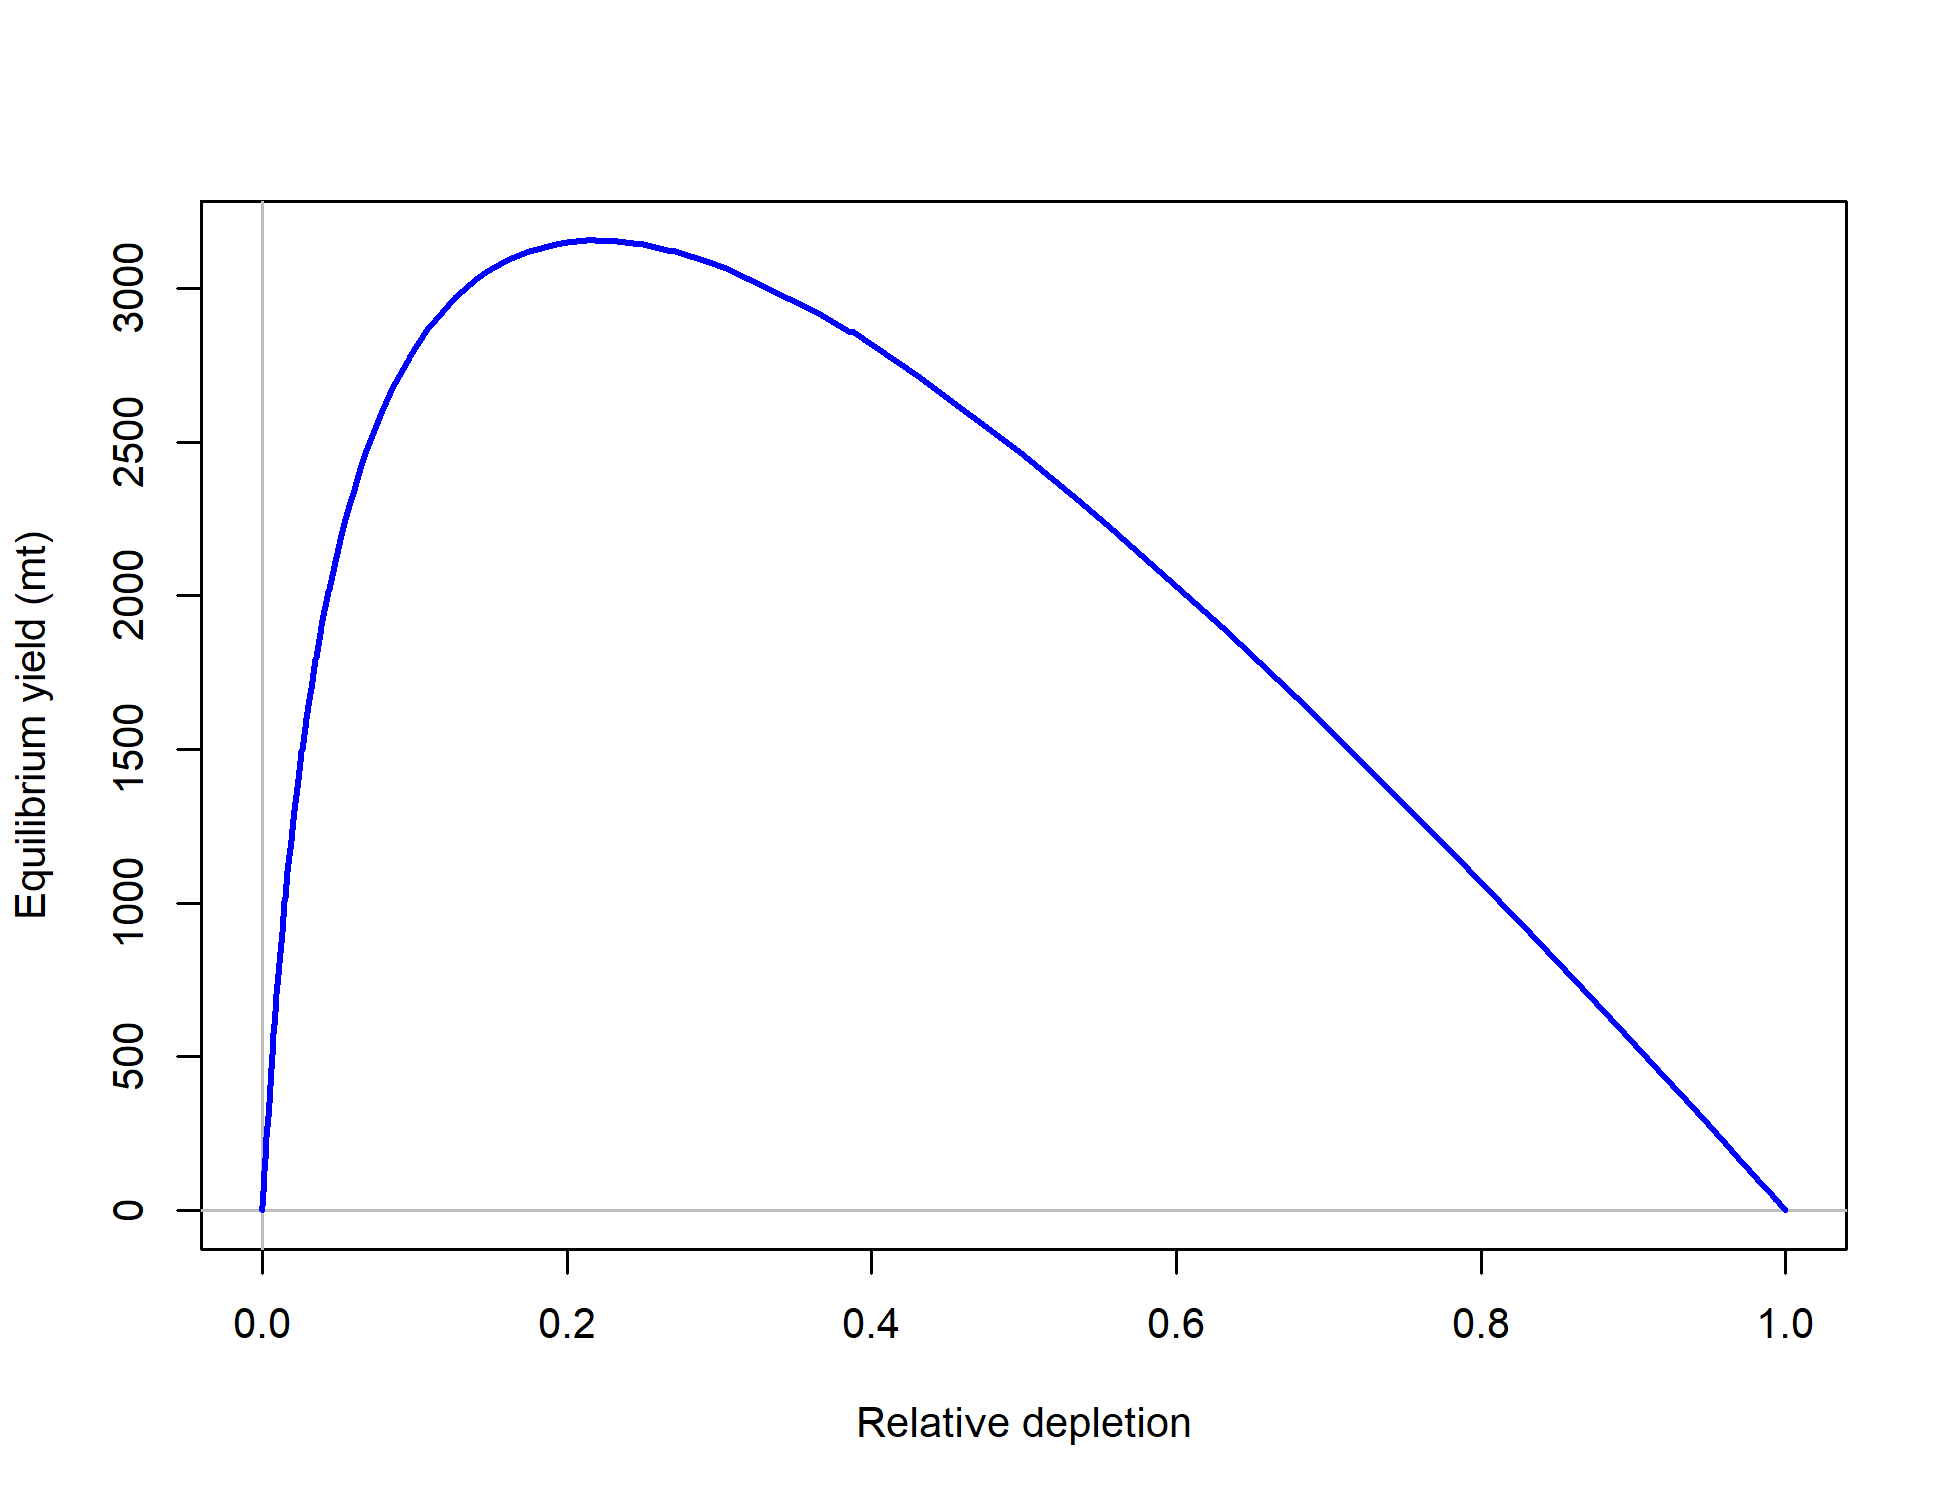
\includegraphics{r4ss/plots_mod1/yield1_yield_curve.png}
\caption{Equilibrium yield curve for the base case model. Values are
based on the 2018 fishery selectivity and with steepness fixed at 0.84.
\label{fig:Yield_all}}
\end{figure}

\FloatBarrier

\newpage

\renewcommand{\thefigure}{\arabic{figure}}
\renewcommand{\thetable}{\arabic{table}}

\setcounter{figure}{0} \setcounter{table}{0}

\pagenumbering{arabic}

\section{Introduction}\label{introduction}

This updated assessment does not attempt to reiterate all background
information for petrale sole presented in the 2013 assessment document.
Instead, only a few key assumptions are restated, along with a detailed
description of changes made during the course of the update. Those
interested in a more complete description of petrale sole life-history
and the details of previous assessments should refer to the 2013
assessment (Haltuch et al.
\protect\hyperlink{ref-haltuch_status_2013}{2013}\protect\hyperlink{ref-haltuch_status_2013}{b}).

\subsection{Basic Information}\label{basic-information}

Petrale sole (\emph{Eopsetta jordani}) is a right-eyed flounder in the
family Pleuronectidae ranging from the western Gulf of Alaska to the
Coronado Islands, northern Baja California (Kramer et al.
\protect\hyperlink{ref-kramer_guide_1995}{1995}, Love et al.
\protect\hyperlink{ref-love_milton_resource_2005}{2005}) with a
preference for soft substrates at depths ranging from 0-550 m (Love et
al. \protect\hyperlink{ref-love_milton_resource_2005}{2005}). Common
names include brill, California sole, Jordan's flounder, cape sole,
round nose sole, English sole, soglia, petorau, nameta, and tsubame
garei (Smith \protect\hyperlink{ref-smith_report_1937}{1937}, Gates and
Frey \protect\hyperlink{ref-gates_designated_1974}{1974}, Eschmeyer and
Herald \protect\hyperlink{ref-eschmeyer_field_1983}{1983}, Love
\protect\hyperlink{ref-love_milton_probably_1996}{1996}). In northern
and central California petrale sole are dominant on the middle and outer
continental shelf. PacFIN fishery logbook data show that adults are
caught in depths from 18 to 1,280 m off the U.S. West Coast with a
majority of the catches of petrale sole being taken between 70-220 m
during March through October, and between 290-440 m during November
through February.

Past assessments completed by Demory
(\protect\hyperlink{ref-demory_progress_1984}{1984},), Turnock et al.
(\protect\hyperlink{ref-turnock_status_1993}{1993}), and Sampson and Lee
(\protect\hyperlink{ref-sampson_assessment_1999}{1999}) considered
petrale sole in the Columbia and U.S.-Vancouver INPFC areas a single
stock. Sampson and Lee (1999) assumed that petrale sole in the Eureka
and Monterey INPFC areas represented two additional distinct socks. The
2005 petrale sole assessment assumed two stocks, northern
(U.S.-Vancouver and Columbia INPFC areas) and southern (Eureka, Monterey
and Conception INPFC areas), to maintain continuity with previous
assessments. Three stocks (West Coast Vancouver Island, Queen Charlotte
Sound, and Heceta Strait) are considered for petrale sole in the waters
off British Columbia, Canada (Starr and Fargo
\protect\hyperlink{ref-starr_petrale_2004}{2004}). The 2009, 2011, 2013,
and 2015 assessments integrate the previously separate north-south
assessments to provide a coast-wide status evaluation. The decision to
conduct a single-area assessment is based on strong evidence of a mixed
stock from tagging studies, a lack of genetic studies on stock
structure, and a lack of evidence for differences in growth between the
2005 northern and southern assessment areas and from examination of the
fishery size-at-age data, as well as confounding differences in data
collection between Washington, Oregon, and California. This 2019 update
assessment provides a coast-wide status evaluation for petrale sole
using data through 2018.

Fishing fleets are separated both geographically and seasonally to
account for spatial and seasonal patterns in catch given the coast-wide
assessment area. The petrale sole fisheries possess a distinct
seasonality, with catches peaking during the winter months, so the
fisheries are divided into winter (November-February) and summer
(March-October) fisheries. Note that the ``fishing year'' for this
assessment (November 1 to October 31) differs from the standard calendar
year. The U.S.-Canadian border is the northern boundary for the assessed
stock, although the basis for this choice is due to political and
current management needs rather than the population dynamics. Given the
lack of clear information regarding the status of distinct biological
populations, this assessment treats the U.S. Petrale sole resource from
the Mexican border to the Canadian border as a single coast-wide stock.

\subsection{Life History}\label{life-history}

Petrale sole spawn during the winter at several discrete deep water
sites (270-460 m) off the U.S. West Coast, from November to April, with
peak spawning taking place from December to February (Harry
\protect\hyperlink{ref-harry_time_1959}{1959}, Best
\protect\hyperlink{ref-best_petrale_1960}{1960}, Gregory and Jow
\protect\hyperlink{ref-gregory_validity_1976}{1976}, Castillo et al.
\protect\hyperlink{ref-castillo_g.c._environmental_1993}{1993}, Reilly
et al. \protect\hyperlink{ref-reilly_recreational_1994}{1994}, Love
\protect\hyperlink{ref-love_milton_probably_1996}{1996}). Females spawn
once each year and fecundity varies with fish size, with one large
female laying as many as 1.5 million eggs (Porter
\protect\hyperlink{ref-porter_notes_1964}{1964}). Petrale sole eggs are
planktonic, ranging in size from 1.2 to 1.3 mm, and are found in deep
water habitats at water temperatures of 4-10 degrees C and salinities of
25-30 ppt (Best \protect\hyperlink{ref-best_petrale_1960}{1960}, Ketchen
and Forrester \protect\hyperlink{ref-ketchen_population_1966}{1966},
Alderdice and Forrest
\protect\hyperlink{ref-alderdice_effects_1971}{1971}, Gregory and Jow
\protect\hyperlink{ref-gregory_validity_1976}{1976}). The duration of
the egg stage can range from approximately 6 to 14 days (Alderdice and
Forrest \protect\hyperlink{ref-alderdice_effects_1971}{1971}, Love
\protect\hyperlink{ref-love_milton_probably_1996}{1996}). The most
favorable conditions for egg incubation and larval growth are 6-7
degrees C and 27.5-29.5 ppt (Ketchen and Forrester
\protect\hyperlink{ref-ketchen_population_1966}{1966}, Alderdice and
Forrest \protect\hyperlink{ref-alderdice_effects_1971}{1971}, Castillo
\protect\hyperlink{ref-castillo_latitudinal_1995}{1995}).

Adult petrale sole achieve a maximum size of around 50 cm and 63 cm for
males and females, respectively (Best
\protect\hyperlink{ref-best_e.a._movements_1963}{1963}, Pedersen
\protect\hyperlink{ref-pedersen_movements_1975}{1975}). The maximum
length reported for petrale sole is 70 cm (Eschmeyer and Herald
\protect\hyperlink{ref-eschmeyer_field_1983}{1983}, Love et al.
\protect\hyperlink{ref-love_milton_resource_2005}{2005}) while the
maximum observed break-and-burn age is 31 years (Haltuch et al.
\protect\hyperlink{ref-haltuch_status_2013}{2013}\protect\hyperlink{ref-haltuch_status_2013}{b}).

\subsection{Historical and Current Fishery
Information}\label{historical-and-current-fishery-information}

Petrale sole have been caught in the flatfish fishery off the U.S.
Pacific coast since the late 19th century. The fishery first developed
off of California where, prior to 1876, fishing in San Francisco Bay was
by hand or set lines and beach seining (Scofield
\protect\hyperlink{ref-scofield_trawling_1948}{1948}). By 1880 two San
Francisco based trawler companies were running a total of six boats,
extending the fishing grounds beyond the Golden Gate Bridge northward to
Point Reyes (Scofield
\protect\hyperlink{ref-scofield_trawling_1948}{1948}). Steam trawlers
entered the fishery during 1888 and 1889, and four steam tugs based out
of San Francisco were sufficient to flood market with flatfish (Scofield
\protect\hyperlink{ref-scofield_trawling_1948}{1948}). By 1915 San
Francisco and Santa Cruz trawlers were operating at depths of about
45-100 m with catches averaging 10,000 lbs per tow or 3,000 lbs per hour
(Scofield \protect\hyperlink{ref-scofield_trawling_1948}{1948}).
Flatfish comprised approximately 90\% of the catch with 20-25\% being
discarded as unmarketable (Scofield
\protect\hyperlink{ref-scofield_trawling_1948}{1948}). During 1915 laws
were enacted that prohibited dragging in California waters and making it
illegal to possess a trawl net from Santa Barbara County southward
(Scofield \protect\hyperlink{ref-scofield_trawling_1948}{1948}). By 1934
twenty 56-72 foot diesel engine trawlers operated out of San Francisco
fishing between about 55 and 185 m (Scofield
\protect\hyperlink{ref-scofield_trawling_1948}{1948}). From 1944-1947
the number of California trawlers fluctuated between 16 and 46 boats
(Scofield \protect\hyperlink{ref-scofield_trawling_1948}{1948}).
Although the flatfish fishery in California was well developed by the
1950s and 1960s, catch statistics were not reported until 1970 (Heimann
and Carlisle \protect\hyperlink{ref-heimann_pacific_1970}{1970}). In
this early California report petrale sole landings during 1916 to 1930
were not separated from the total flatfish landings.

The earliest trawl fishing off Oregon began during 1884-1885, and the
fishery was solidly established by 1937, with the fishery increasing
rapidly during WWII (Harry and Morgan, 1961). Initially trawlers stayed
close to the fishing grounds adjacent to Newport and Astoria, operating
at about 35-90 m between Stonewall Bank and Depoe Bay. Fishing
operations gradually extended into deep water. For example,
Newport-based trawlers were commonly fishing at about 185 m in 1949, at
about 185-365 m by 1952, and at about 550 m by 1953.

Alverson and Chatwin
(\protect\hyperlink{ref-alverson_results_1957}{1957}) describe the
history of the petrale sole fishery off of Washington and British
Columbia with fishing grounds ranging from Cape Flattery to Destruction
Island. Petrale sole catches off of Washington were small until the late
1930s with the fishery extending to about 365 m following the
development of deep water rockfish fisheries during the 1950s.

By the 1950s the petrale sole fishery was showing signs of depletion
with reports suggesting that petrale sole abundance had declined by at
least 50\% from 1942 to 1947 (Harry
\protect\hyperlink{ref-harry_analysis_1956}{1956}). Sampson and Lee
(\protect\hyperlink{ref-sampson_assessment_1999}{1999}) reported that
three fishery regulations were implemented during 1957-67: 1) a winter
closure off Oregon, Washington and British Columbia, 2) a 3,000 lb per
trip limit, and 3) no more than two trips per month during 1957. With
the 1977 enactment of the Magnuson Fishery Conservation and Management
Act (MFCMA) the large foreign-dominated fishery that had developed since
the late 1960s was replaced by the domestic fishery that continues
today. Petrale sole are harvested almost exclusively by bottom trawls in
the U.S. West Coast groundfish fishery. Recent petrale sole catches
exhibit marked seasonal variation, with substantial portions of the
annual harvest taken from the spawning grounds during December and
January. Evidence suggests that the winter fishery on the deep water
spawning grounds developed sporadically during the 1950s and 1960s as
fishers discovered new locations (e.g., Alverson and Chatwin
(\protect\hyperlink{ref-alverson_results_1957}{1957}); Ketchen and
Forrester (\protect\hyperlink{ref-ketchen_population_1966}{1966})). Both
historical and current petrale sole fisheries have primarily relied upon
trawl fleets. Fishery removals were divided among 4 fleets: 1) winter
North trawl, 2) summer North trawl, 3) winter South trawl, and 4) summer
South trawl. Landings for the North fleet are defined as fish landed in
Washington and Oregon ports. Landings for the South fleet are defined as
fish landed in California ports.

Historical landings reconstructions show peak catches from the summer
fishery occurred during the 1940s and 1950s and subsequently declined,
during which time the fleet moved to fishing in deeper waters during the
winter. After the period of peak landings during the 1940s and 1950s,
total landings were somewhat stable until about the late 1970s, and then
generally declined until the mid-2000s. (Table \ref{tab:Comm_Catch},
Figure \ref{fig:Catch}). During 2009 the fishery was declared overfished
and during 2010 management restrictions limited the catch to 755 mt
(Table \ref{tab:Comm_Catch}, Figure \ref{fig:Catch}). Recent years
overfishing limit (OFL), annual catch limit (ACL), landings, and
estimated total dead are shown in Table \ref{tab:mnmgt_perform_tables}.

\subsection{Summary of Management History and
Performance}\label{summary-of-management-history-and-performance}

Beginning in 1983 the Pacific Fishery Management Council (PFMC)
established coast-wide annual catch limits (ACLs) for the annual
harvests of petrale sole in the waters off the U.S. West Coast. The
first assessment of West Coast petrale sole occurred in 1984 (Demory
\protect\hyperlink{ref-demory_progress_1984}{1984}). Based on the 1999
assessment a coast-wide ACL of 2,762 mt was specified and remained
unchanged between 2001 and 2006.

The 2005 assessment of petrale sole stock assessment split the stock
into two areas, the northern area that included U.S.-Vancouver and
Columbia INPFC areas and the southern area that included the Eureka,
Monterey and Conception INPFC areas (Lai et al.
\protect\hyperlink{ref-lai_stock_2005}{2005}). While petrale sole stock
structure is not well understood, CPUE and geographical differences
between states were used to support the use of two separate assessment
areas. In 2005 petrale sole were estimated to be at 34 and 29\% of
unfished spawning stock biomass in the northern and southern areas,
respectively. In spite of different models and data, the biomass trends
were qualitatively similar in both areas, providing support for a
coast-wide stock. This assessment estimated that petrale sole had
historically been below the Pacific Council's minimum stock size
threshold of 25\% of unfished biomass from the mid-1970s until just
prior to the completion of the assessment, with estimated harvest rates
in excess of the target fishing mortality rate implemented for petrale
sole at that time (F40\%). However, the 2005 stock assessment determined
that the stock was in the precautionary zone and was not overfished
(i.e., the spawning stock biomass was not below 25\% of the unfished
spawning stock biomass). Based on the 2005 stock assessment results,
ACLs were set at 3,025 mt and 2,919 mt for 2007 and 2008, respectively,
with an ACT of 2,499 mt for both years.

In comparison to the 1999 assessment of petrale sole, the 2005
assessment represented a significant change in the perception of petrale
sole stock status. The stock assessment conducted in 1999
(Washington-Oregon only) estimated the spawning stock biomass in 1998 at
39\% of unfished stock biomass. Although the estimates of 1998
spawning-stock biomass were little changed between the 1999 and 2005
(Northern area) assessments, the estimated depletion in the 2005
assessment was much lower. The change in status between the 1999 and
2005 analyses was due to the introduction of a reconstructed catch
history in 2005, which spanned the entire period of removals. The 1999
stock assessment used a catch history that started in 1977, after the
bulk of the removals from the fishery had already taken place. Thus the
1999 stock assessment produced a more optimistic view of the petrale
stock's level of depletion. The stock's estimated decline in status
between the 2005 and 2009 assessments was driven primarily by a
significant decline in the trawl-survey index over that period. The 2011
assessment concluded that the stock status continued to be below the
target of 25\% of unfished biomass.

The 2009 coast-wide stock assessment estimated that the petrale sole
stock had declined from its 2005 high to 11.6\% of the unfished spawning
stock biomass (Haltuch and Hicks
\protect\hyperlink{ref-haltuch_status_2009}{2009}). The petrale sole was
declared overfished based on newly adopted management targets (e.g.,
target spawning biomass for flatfish stocks defined as 25\% and
overfished threshold of 12.5\% of unfished spawning stock biomass)
resulting in a rebuilding plan and catch restrictions for petrale sole.
The stock was declared rebuilt based on the results of the 2015 update
stock assessment which estimated the coastwide biomass at 30.7\% of
unfished spawning stock output with ACLs of 3,136 and 3,013 in 2017 and
2018 respectively (Stawitz et al.
\protect\hyperlink{ref-stawitz_stock_2015}{2015}).

For additional information on changes in the petrale sole fishery please
see the 2013 stock assessment (Haltuch et al.
\protect\hyperlink{ref-haltuch_status_2013}{2013}\protect\hyperlink{ref-haltuch_status_2013}{b}).

\subsection{Fisheries off Canada and
Alaska}\label{fisheries-off-canada-and-alaska}

The Canadian fishery developed rapidly during the late 1940s to
mid-1950s following the discovery of petrale sole spawning aggregations
off the West Coast of Vancouver Island (Anon
\protect\hyperlink{ref-anon_fish_2001}{2001}). Annual landings of
petrale sole in British Columbia peaked at 4,800 mt in 1948 but declined
significantly after the mid-1960s (Anon
\protect\hyperlink{ref-anon_fish_2001}{2001}). By the 1970s, analysis
conducted by Pederson
(\protect\hyperlink{ref-pedersen_movements_1975}{1975}) suggested that
petrale sole abundance was low and abundance remained low into the
1990s. In the early 1990s vessel trip quotas were established to try to
halt the decline in petrale sole abundance (Anon
\protect\hyperlink{ref-anon_fish_2001}{2001}). Winter quarter landings
of petrale sole were limited to 44,000 lb per trip during 1985-91; to
10,000 lb per trip during 1991-95; and to 2,000 lb per trip in 1996.
Biological data collected during 1980-1996 showed a prolonged decline in
the proportion of young fish entering the population (Anon
\protect\hyperlink{ref-anon_fish_2001}{2001}). Therefore, no directed
fishing for petrale sole has been permitted in Canada since 1996 due to
a continuing decline in long term abundance (Fargo
\protect\hyperlink{ref-fargo_j.j._flatfish_1997}{1997}, Anon
\protect\hyperlink{ref-anon_fish_2001}{2001}). As of 2005 petrale sole
off of British Columbia were treated as three ``stocks'' and were still
considered to be at low levels. The recent assessments for the Canadian
stocks have been based on catch histories and limited biological data.

In Alaska petrale sole are not targeted in the Bering Sea/Aleutian
Island fisheries and are managed as a minor species in the ``Other
Flatfish'' stock complex.

\section{Data}\label{data}

Data used in the petrale sole assessment are summarized in Figure
\ref{fig:data_plot}. The data that were added or reprocessed for this
assessment are:

\begin{enumerate}
  \item Commercial catches (2015-2018 added);
  \item Commercial length and age data (all years reprocessed, 2015-2018 added);
  \item Observed discard rates, average weights, and lengths (2002-2017 reprocessed, 2014-2017 added); 
  \item AFSC/NWFSC West Coast Triennial Shelf Survey early and late indices of abundance and length composition data (1980-2004 reprocessed); and
  \item NWFSC West Coast Groundfish Bottom Trawl Survey index of abundance, length and age composition data (2003-2018 reprocessed, 2015-2018 added).
\end{enumerate}

A description of each data source is provided below.

\subsection{Fishery-Independent Data}\label{fishery-independent-data}

\subsubsection{NWFSC West Coast Groundfish Bottom Trawl
Survey}\label{nwfsc-west-coast-groundfish-bottom-trawl-survey}

Three sources of information are produced by this survey: an index of
relative abundance, length-frequency distributions, and age-frequency
distributions. Only years in which the NWFSC West Coast Groundfish
Bottom Trawl Survey included the continental shelf (55-183 m) are
considered (2003-2018), since the highest percent of positive survey
tows with petrale sole are found on the continental shelf.

The NWFSC West Coast Groundfish Bottom Trawl Survey is based on a
random-grid design; covering the coastal waters from a depth of 55 m to
1,280 m (Bradburn et al.
\protect\hyperlink{ref-bradburn_2003_2011}{2011}). This design uses four
industry chartered vessels per year, assigned to a roughly equal number
of randomly selected grid cells and divided into two `passes' of the
coast that are executed from north to south. Two vessels fish during
each pass, which are conducted from late May to early October each year.
This design therefore incorporates both vessel-to-vessel differences in
catchability as well as variance associated with selecting a relatively
small number (\textasciitilde{}700) of possible cells from a very large
set of possible cells spread from the Mexican to the Canadian border.

The NWFSC West Coast Groundfish Bottom Trawl Survey commonly encounters
petrale sole along the U.S West Coast, except south of Point Conception
(Figure \ref{fig:nw_map}). The catch-per-unit-effort estimated from the
survey is roughly constant north of 38\(^\circ\) (Figure
\ref{fig:nw_cpue_lat}). The survey does fish shallower than 54 m and no
petrale sole were caught deeper than 550 m. Figure
\ref{fig:nw_cpue_depth} shows that the postie tows catch rate by depth
peaks between 100-200 meters and declines as depth increases.

The data from the NWFSC West Coast Groundfish Bottom Trawl Survey was
analyzed using a spatio-temporal delta model implemented as an R
package, VAST (Thorson and Barnett
\protect\hyperlink{ref-thorson_comparing_2017}{2017}), which is publicly
available online (\url{https://github.com/James-Thorson/VAST}). Spatial
and spatio-temporal variation is specifically included in both encounter
probability and positive catch rates, a logit-link for encounter
probability and a log-link for positive catch rates. Vessel-year effects
were included for each unique combination of vessel and year in the data
to account for the random selection of commercial vessels used during
sampling (Helser et al.
\protect\hyperlink{ref-helser_generalized_2004}{2004}, Thorson and Ward
\protect\hyperlink{ref-thorson_accounting_2013}{2013}). Spatial
variation was approximated using 250 knots, and the model used the
bias-correction algorithm (Thorson and Kristensen
\protect\hyperlink{ref-thorson_implementing_2016}{2016}) in Template
Model Builder (Kristensen et al.
\protect\hyperlink{ref-kristensen_tmb:_2016}{2016}). Further details
regarding model structure are available in the user manual
(\url{https://github.com/James-Thorson/VAST/blob/} master/examples/VAST
user manual.pdf). The stratification is provided in Table
\ref{tab:strata_nwfsc}.

The estimated index of abundance is shown in Table
\ref{tab:Index_Summary}. For contrast, the 2015 model estimated, the
2019 design based, and the 2019 VAST indices are shown in Figure
\ref{fig:nw_index}. The lognormal distribution with random strata-year
and vessel effects had the lowest AIC and was chosen as the final model.
The Q-Q plot does not show any departures from the assumed distribution
(Figure \ref{fig:nw_qq}). The index for the NWFSC West Coast Groundfish
Bottom Trawl Survey shows an increase in the population between 2009 and
2014 and roughly stable through 2017, and decrease in the most recent
year.

Length bins from 12 to 62 cm in 2 cm increments were used to summarize
the length frequency of the survey catches in each year. Table
\ref{tab:NWcombo_Lengths} shows the number of lengths taken by the
survey. The first bin includes all observations less than 14 cm and the
last bin includes all fish larger than 62 cm. The length frequency
distributions for the NWFSC West Coast Groundfish Bottom Trawl Survey
from 2003-2018 generally show a strong cohort growing through 2005 and
smaller fish entering the population beginning in 2007 rows with a large
2014 cohort entering the populations (Figure \ref{fig:nw_len_freq}).

Age distributions included bins from age 1 to age 17, with the last bin
including all fish of greater age. Table \ref{tab:NWcombo_Ages} shows
the number of ages taken by the survey. The marginal NWFSC West Coast
Groundfish Bottom Trawl Survey age-compositions, which allow for easier
viewing of strong cohorts, show the strong 1998 cohort ageing from 2003
to 2007, with younger fish appearing between 2008-2014 (Figure
\ref{fig:nw_age_freq}). The exception to this is the female composition
in 2005, where only one female fish was aged from the tow with the
largest catch rate. The expansion of numbers to tow can greatly affect
the marginal age distribution, but does not have as much effect on the
conditional age-at-length data.

The input sample sizes for length and marginal age-composition data for
all fishery-independent surveys were calculated based on the approach
used in the 2013 full and 2015 update assessment as:

\begin{centering}

$N = (0.138*(\sum_{}^{N} fish_{y} / \sum_{}^N tows_{y}) + 1)*\sum_{}^N tows_y$ 

\end{centering}

where fish is the number of petrale sole by year \(y\) and the total
number of tows by year. The effective sample size of
conditional-age-at-length data was set at the number of fish at each
length by sex and by year. The conditional-age-at-length data were not
expanded and were binned by according to length, age, sex, and year.

\subsubsection{AFSC/NWFSC West Coast Triennial Shelf
Survey}\label{afscnwfsc-west-coast-triennial-shelf-survey}

The AFSC/NWFSC West Coast Triennial Shelf Survey (referred to as the
Triennial Survey for short) was first conducted by the AFSC in 1977 and
spanned the time-frame from 1977-2004. The survey's design and sampling
methods are most recently described in Weinberg et al.
(\protect\hyperlink{ref-weinberg_2001_2002}{2002}). Its basic design was
a series of equally-spaced transects from which searches for tows in a
specific depth range were initiated. The survey design has changed
slightly over the period of time. In general, all of the surveys were
conducted in the mid-summer through early fall: the 1977 survey was
conducted from early July through late September; the surveys from 1980
through 1989 ran from mid-July to late September; the 1992 survey
spanned from mid-July through early October; the 1995 survey was
conducted from early June to late August; the 1998 survey ran from early
June through early August; and the 2001 and 2004 surveys were conducted
in May-July.

Haul depths ranged from 91-457 m during the 1977 survey with no hauls
shallower than 91 m. The surveys in 1980, 1983, and 1986 covered the
West Coast south to \(36.8^\circ\) N latitude and a depth range of
55-366 m. The surveys in 1989 and 1992 covered the same depth range but
extended the southern range to \(34.5^\circ\) N (near Point Conception).
From 1995 through 2004, the surveys covered the depth range 55-500 m and
surveyed south to \(34.5^\circ\) N. In the final year of the Triennial
Survey series, 2004, the NWFSC's Fishery Resource and Monitoring
division (FRAM) conducted the survey and followed very similar protocols
as the Alaska Fisheries Science Center (AFSC).

Due to changes in survey timing, the Triennial Survey data have been
split into independent early (1980-1992) and late (1995-2004) survey
time series. The splitting of this time series was investigated during
the 2009 STAR panel due to the changes in survey timing and the expected
change in petrale sole catchability because of the stock's seasonal
onshore-offshore migrations (Cook et al.
\protect\hyperlink{ref-cook_petrale_2009}{2009}). For these reasons, as
well as because the split improved fits to the split time series and
made small changes to the estimation of the selectivity curves, the 2009
STAR panel supported the split.

The Triennial Survey commonly encounters petrale sole along the U.S West
Coast (Figure \ref{fig:tri_map}). The catch-per-unit-effort estimated
from the survey is roughly constant across the surveyed latitudes
(Figure \ref{fig:tri_cpue_lat}). Additionally, petrale sole were
captured across the survey depths between 55-500 m (Figure
\ref{fig:tri_cpue_depth}).

The data from the petrale sole was analyzed using a spatio-temporal
delta model implemented as an R package, VAST (Thorson and Barnett
\protect\hyperlink{ref-thorson_comparing_2017}{2017}), described above
in Section \ref{nwfsc-west-coast-groundfish-bottom-trawl-survey}.
Spatial variation was approximated using 250 knots, and the model used
the bias-correction algorithm (Thorson and Kristensen
\protect\hyperlink{ref-thorson_implementing_2016}{2016}) in Template
Model Builder (Kristensen et al.
\protect\hyperlink{ref-kristensen_tmb:_2016}{2016}). The index of
abundance was estimated using VAST seperately for the early and late
periods of the survey. The stratifications are provided in Tables
\ref{tab:strata_tri_early} and \ref{tab:strata_tri_late}.

The estimated index of abundance is shown in Table
\ref{tab:Index_Summary}. For contrast, the 2015 model estimated, the
2019 design based, and the 2019 VAST indices are shown in Figure
\ref{fig:tri_index}. The lognormal distribution with random strata-year
and vessel effects had the lowest AIC and was chosen as the final model
for both the early and late time periods. The Q-Q plots do not show any
departures from the assumed distribution (Figures \ref{fig:tri_early_qq}
and \ref{fig:tri_late_qq}). The index for the Triennial Survey across
the early and late period shows an slight increase in the population
between 1980 and 2001 with a spike in the final year of 2004.

Length bins from 12 to 62 cm in 2 cm increments were used to summarize
the length frequency of the survey catches in each year. Table
\ref{tab:Triennial_Lengths} shows the number of lengths taken by the
survey. The first bin includes all observations less than 14 cm and the
last bin includes all fish larger than 62 cm. The length frequency
distributions for the Triennial Survey from 1980-2004 are shown in
Figures \ref{fig:tri_early_len_freq} and \ref{fig:tri_late_len_freq}.

There are no petrale sole age data from the Triennial Survey.

The input sample sizes for length data were calculated using the same
approach for the NWFSC West Coast Groundfish Bottom Trawl Survey data
described in Section
\ref{nwfsc-west-coast-groundfish-bottom-trawl-survey}.

\subsection{Fishery-Dependent Data}\label{fishery-dependent-data}

\subsubsection{Commercial Fishery
Landings}\label{commercial-fishery-landings}

All landings for this update assessment were summarized by port of
landing, where available, as well as for a northern fleet consisting of
Washington and Oregon and a southern fleet consisting of California.
Landings for Washington and Oregon are summed into a single northern
fleet due to the fact that vessels commonly fish and land in each
other's waters and ports.

The PacFIN database (1981-2018 for California and Washington; 1987-2018
for Oregon) extracted XXX ADD DATE XXX. Historical catches were not
updated from the previous assessment in 2013. The 2013 assessment
historical Washington catches were obtained from WDFW landings
reconstruction for 1935, 1939 and 1949- 1969 (pers. comm. T. Tsou and G.
Lippert) and the Pacific Marine Fisheries Commission (PMFC) Data Series
for 1956-1980 (PFMC \protect\hyperlink{ref-pfmc_data_1979}{1979}). The
2013 assessment historical Oregon landings were obtained from
reconstruction for 1932 to 1986 (Karnowski et al.
\protect\hyperlink{ref-karnowski_historical_2014}{2014}). The 2013
assessment historical California landings used catch reconstruction data
extending from 1931-1980 (Ralston et al.
\protect\hyperlink{ref-ralston_documentation_2010}{2010}) and California
Department of Fish and Game (CDFG) Fish Bulletins for 1916-1930 landings
(Heimann and Carlisle
\protect\hyperlink{ref-heimann_pacific_1970}{1970}) as reconstructed by
Lai et al. (\protect\hyperlink{ref-lai_stock_2005}{2005}). The
California fishery began in 1876 but no landings data are available from
1876-1915. Therefore a linear interpolation between landings of 1 ton in
1876 and the landings recorded for 1916 are used to filling this period.

Landings for the fishing year, beginning on 1 November, are summarized
by fleet in Table \ref{tab:Comm_Catch} and Figure \ref{fig:Catch}. The
landings of petrale sole by gear types other than groundfish-trawl have
been inconsequential, averaging less than 2.5\% of the coast-wide
landings. The non-trawl landings are included in the trawl landings.

\subsubsection{Discards}\label{discards}

Data on discards of petrale sole are available from two different data
sources. The earliest source is referred to as the Pikitch data and
comes from a study organized by Ellen Pikitch that collected trawl
discards from 1985-1987 (Pikitch et al.
\protect\hyperlink{ref-pikitch_evaluation_1988}{1988}). The northern and
southern boundaries of the study were \(48^\circ 42^\prime\) N latitude
and \(42^\circ 60^\prime\) N latitude respectively, which is primarily
within the Columbia INPFC area (Pikitch et al.
\protect\hyperlink{ref-pikitch_evaluation_1988}{1988}, Rogers and
Pikitch \protect\hyperlink{ref-rogers_numerical_1992}{1992}).
Participation in the study was voluntary and included vessels using
bottom, midwater, and shrimp trawl gears. Observers of normal fishing
operations on commercial vessels collected the data, estimated the total
weight of the catch by tow, and recorded the weight of species retained
and discarded in the sample. Results of the Pikitch data were obtained
from John Wallace (personal communication, NWFSC, NOAA) in the form of
ratios of discard weight to retained weight of petrale sole and
sex-specific length frequencies. The Pikitch discard estimates were
applied to both the summer and winter northern fisheries and are shown
in Table \ref{tab:Discard}.

The second source is from the West Coast Groundfish Observer Program
(WCGOP). This program is part of the NWFSC and has been recording
discard observations since 2003. Table \ref{tab:Discard} shows the
discard ratios (discarded/(discarded + retained)) of petrale sole from
WCGOP. Since 2011, when the trawl rationalization program was
implemented, observer coverage rates increased to nearly 100\% for all
the limited entry trawl vessels in the program and discard rates
declined compared to pre-2011 rates. Discard rates were obtained for
both the catch-share and the non-catch share sector for petrale sole. A
single discard rate was calculated by weighting discard rates based on
the commercial landings by each sector. Coefficient of variations were
calculated for the non-catch shares sector and pre-catch share years by
bootstrapping vessels within ports because the observer program randomly
chooses vessels within ports to be observed. The discard rates from
WCGOP are shown in Table \ref{tab:Discard}.

Starting in 2015 a small number of vessels switched to electronic
monitoring discards at sea (4, 7, and 8 vessels in 2015, 2016, and 2017
respectively) rather than a human observer and as of this update
assessment only 3 years of data are available. Discarding rates at sea
of petrale sole by these vessels were very low, near zero. This update
assessment did not evaluate these data to estimate an electronic
monitoring specific discard rate, but rather applied the discard ratio
from the observed vessels in the WCGOP database. Future assessments
should evaluate this assumption in greater detail.

Discard mean body weight data were obtained from the WCGOP data and used
in this update assessmet for each of the four fishing fleets. The mean
body weight of discarded fish from each fleet are shown in Figures
\ref{fig:nw_bodywt} - \ref{fig:ss_bodywt}. The summer fisheries, both
north and south, had relatively large sample numbers which is reflected
in a lower CV by year relative to the winter fisheries.

Discard length composition data were obtained from the WCGOP data and
used in this update assessment to estimate retention curves for each of
the four fishing fleets. The discard length data from each fleet are
shown in Figures \ref{fig:north_lengths} and \ref{fig:south_lengths}.

The data, historical and current, provided by the WCGOP are updated
annually based on the most recent standards of QA/QC methods. Hence,
these data can have minor changes over time. To ensure the data from the
years since the last update assessment (2014-2018) were consistent with
the earlier data, data from all years were replaced based to reflect the
current standings of the WCGOP data.

\subsubsection{Foreign Landings}\label{foreign-landings}

The impact of landings of petrale sole by foreign fishing fleets prior
to the institution of the exclusive economic zone (EEZ) of the U.S. West
Coast is currently not quantified and remains an area for research.

\subsubsection{Historical Commercial Catch-Per-Unit
Effort/Logbooks}\label{historical-commercial-catch-per-unit-effortlogbooks}

Commercial logbook data for petrale sole was first used to construct
CPUE indices of abundance in the 1999 assessment for Oregon fleets from
1987-1997 (Sampson and Lee
\protect\hyperlink{ref-sampson_assessment_1999}{1999}). Since the first
inclusion 1999, the commercial CPUE indices were extended and or updated
based on management changes and new statistical methods through 2009.
For additional information on the use of CPUE indices in the assessment
of petrale sole please see the 2013 assessment (Haltuch et al.
\protect\hyperlink{ref-haltuch_status_2013}{2013}\protect\hyperlink{ref-haltuch_status_2013}{b}).

CPUE calculations for the Winter fishery on aggregations of petrale sole
described in the 2013 assessment were retained for this assessment
(Haltuch et al.
\protect\hyperlink{ref-haltuch_status_2013}{2013}\protect\hyperlink{ref-haltuch_status_2013}{b})
(Figures \ref{fig:north_cpue} and \ref{fig:south_cpue}). Two CPUE
indices from 1987-2009 with catchability modeled as a power function are
used in this update assessment, one for the north and south winter
fisheries.

\subsubsection{Fishery Length and Age
Data}\label{fishery-length-and-age-data}

The PacFIN BDS database contains data from Oregon Department of Fish and
Wildlife (ODFW; 1966-present) and Washington Department of Fish and
Wildlife (WDFW; 1955- present), but only 1986-present data from
California Department of Fish and Game (CDFG). The CDFG data set for the
years 1948-1992 was extracted and provided from CALCOM by Brenda Erwin
(CDFG) in 2011.

Commercial length-frequency distributions based on the fishing year were
developed for each state for which observations were available. For each
fleet, the raw observations (compiled from the PacFIN and CalCOM
databases) were expanded to the sample level, to allow for any fish that
were not measured, then to the trip level to account for the relative
size of the landing from which the sample was obtained. The expanded
length observations were then expanded by the landings in each state for
the combined Washington and Oregon fleet. Age frequencies were computed
in the same manner, except that age observations for Washington and
Oregon were not combined due to aging error considerations.

Length and age data collected from commercial landings for each fleet
are summarized by the number of trips and fish sampled by year (Tables
\ref{tab:Fishery_Lengths} and \ref{tab:Fishery_Ages}). Figures
\ref{fig:north_lengths}, \ref{fig:south_lengths}, and
\ref{fig:comm_ages} show plots of the commercial length and age
composition data across time for each fishery fleet.

The calculation for input sample sizes for the commercial length and age
data was done to be consistent with the 2015 update assessment. The
input sample size for commercial lengths and ages were set equal to the
number of trips by year for each fleet.

\subsection{Biological Data}\label{biological-data}

\subsubsection{Natural Mortality}\label{natural-mortality}

The instantaneous rate of natural mortality for a wild fish population
is notoriously difficult to estimate. One accepted method is to examine
the age distribution of an unexploited or lightly exploited stock. This
method cannot readily be applied to petrale sole given the long history
of exploitation off the U.S. West Coast. Ketchen and Forrester
(\protect\hyperlink{ref-ketchen_population_1966}{1966}) estimated that
the natural mortality coefficients were 0.18-0.26 yr\textsuperscript{-1}
for males and 0.19-0.21 yr\textsuperscript{-1} for females based on a
catch curve analysis of 1943-1945 Washington trawl data from Swiftsure
Bank, off the southwest corner of Vancouver Island. However, petrale
sole catches were relatively high during mid-1940s through the 1950s.
Starr and Fargo (\protect\hyperlink{ref-starr_petrale_2004}{2004})
estimated the instantaneous rate of natural mortality (\(M\)) using
Hoenig's method (Hoenig
\protect\hyperlink{ref-hoenig_empirical_1983}{1983}) estimating \(M\)
values of 0.22 and 0.15 yr\textsuperscript{-1} were estimated given
maximum ages of 20 and 30 years, respectively.

An archived set of commercial samples, collected from Northern
California between the late 1950s and early 1980s, recently found that
multiple samples were aged between 20-31 years old, suggesting a similar
range of \(M\) values for U.S. West Coast petrale sole. U.S. stock
assessments prior to 2009 and current British Columbia stock assessments
assumed a value of \(M\) = 0.2 yr\textsuperscript{-1} for both sexes.
The 2013 stock assessment used a meta-analysis value produced the
following normal prior distributions for females (mean = 0.151, sd =
0.16) and males (0.206, sd = 0.218) based on early research by Owen
Hamel (pers. comm.) with maximum age for females and males of 32 and 29
years, respectively.

Hamel (\protect\hyperlink{ref-hamel_method_2015}{2015}) refined and
published a method for combining meta-analytic approaches relating the
\(M\) rate to other life-history parameters such as longevity, size,
growth rate, and reproductive effort to provide a prior on \(M\). In
that same issue of \emph{ICES Journal of Marine Science}, Then et al.
(\protect\hyperlink{ref-then_evaluating_2015}{2015}) provided an updated
data set of estimates of \(M\) and related life history parameters
across a large number of fish species from which to develop an \(M\)
estimator for fish species in general. They concluded by recommending
\(M\) estimates be based on maximum age alone, based on an updated
Hoenig non-linear least squares estimator \(M=4.899A^{-0.916}_{max}\).
The approach of basing \(M\) priors on maximum age alone was one that
was already being used for West Coast rockfish assessments. However, in
fitting the alternative model forms relating \(M\) to
\(A_{\text{max}}\), Then et al.
(\protect\hyperlink{ref-then_evaluating_2015}{2015}) did not
consistently apply their transformation. In particular, in real space,
one would expect substantial heteroscedasticity in both the observation
and process error associated with the observed relationship of \(M\) to
\(A_{\text{max}}\). Therefore, it would be reasonable to fit all models
under a log transformation. This was not done. Re-evaluating the data
used in Then et al. (\protect\hyperlink{ref-then_evaluating_2015}{2015})
by fitting the one-parameter \(A_{\text{max}}\) model under a log-log
transformation (such that the slope is forced to be -1 in the
transformed space (Hamel
\protect\hyperlink{ref-hamel_method_2015}{2015})), the point estimate
for \(M\) is:

\begin{centering}

$M=\frac{5.4}{A_{\text{max}}}$

\end{centering}

The above is also the median of the prior. The prior is defined as a
lognormal distribution with mean \(ln(5.4/A_{\text{max}})\) and SE =
0.438.

The natural mortality prior was updated for this update assessment using
the above approach. Maximum age was assumed to be 32 and 29 years for
females and males, respectively, the same assumption applied in the 2013
assessment. Using the Hamel et al. approach above, the prior value for
females in regular space is 0.169 and for males is 0.186.

\subsubsection{Maturation and Fecundity}\label{maturation-and-fecundity}

Petrale sole maturity-at-length information is generally sparse in space
and time, has not been collected in a systematic fashion across time, is
of varying quality, and does not always agree between studies. It is
possible that maturity may have changed over time. However, it is not
possible to assess this quantitatively owing to differences in when
historical samples on which maturity ogives could be based were taken,
and how maturity stage (visual vs.~histological) was determined. The
2005 petrale sole assessment used the most recent study for the West
Coast of the U.S. that was based on observations collected during 2002
from Oregon and Washington (Hannah et al.
\protect\hyperlink{ref-hannah_length_2002}{2002}). The 50\%
size-at-maturity was estimated at 33.1 cm with maturity asymptoting to
1.0 for larger fish (Figure \ref{fig:maturity}).

To date, there has been limited information regarding fecundity at age
or length of petrale sole. The 2013 stock assessment assumed that
fecundity of female petrale sole was equal to biomass (Figure
\ref{fig:fecundity_model}). Since the last full assessment, new research
has been done examining the fecundity of petrale sole (Lefebvre et al.
in press). The study concluded a difference in fecundity between
California and Washington petrale sole where a 40 cm fish in California
is more fecund compared to northern fish of the same size (Figure
\ref{fig:fecundity}). However, northern fish of the largest size were
more fecund relative to fish in California. The current petrale sole
model is a single area coastwide model, which assumes fish along the
U.S. have the same biology (e.g.~natural mortality, growth, fecundity).
The estimates of fecundity for petrale sole were considered new data and
based on the guidelines for update stock assessments, these data were
not included in the base model. However, a sensitivity to including
these data was provided. The next full assessment should include the new
data about fecundity at length.

\subsubsection{Sex Ratio}\label{sex-ratio}

Past assessments of petrale sole have assumed a 50\% sex ratio between
females and males off the U.S West Coast. Similarly, Canadian data from
the 2004 published stock assessment also suggests sex ratios of petrale
sole in British Columbia are generally 50\% males and 50\% females
(Starr and Fargo \protect\hyperlink{ref-starr_petrale_2004}{2004}). To
be consistent with the full assessment this update assessment retains
the equal sex ratio assumption. However, examining the NWFSC West Coast
Groundfish Bottom Trawl Survey data the proportion of females in the
population across the mid-range lengths is approximately 0.40 with the
proportion increasing to 1 at the largest lengths due to dimorphic
growth (Figure \ref{fig:sex_ratio}). The next full assessment should
evaluate the sex ratio for petrale sole.

\subsubsection{Length-Weight
Relationship}\label{length-weight-relationship}

The length-weight relationship for petrale sole was estimated outside
the model using all biological data available from the NWFSC West Coast
Groundfish Bottom Trawl Survey data, where the female weight-at-length
in grams was estimated at 2.08e-06\(L\)\textsuperscript{3.47} and males
at 3.05e-06\(L\)\textsuperscript{3.36} where \(L\) is length in cm
(Figures \ref{fig:wt_length}).

\subsubsection{Growth (Length-at-Age)}\label{growth-length-at-age}

The length-at-age was estimated for male and female petrale sole. Figure
\ref{fig:length_age} shows the lengths and ages as well as predicted von
Bertalanffy fits to the data from the fishery and the NWFSC West Coast
Groundfish Bottom Trawl Survey data. Females grow larger than males and
sex-specific growth parameters were estimated at the following values:

XXX DOUBLE CHECK THESE VALUES WHEN AGES ARRIVE XXX

\begin{centering}

Females $L_{\infty}$ = 54; $k$ = 0.16

Males $L_{\infty}$ = 41; $k$ = 0.25

\end{centering}

These values were used as starting parameter values within the base
model prior to estimating each parameter for male and female petrale
sole.

\subsubsection{Ageing Precision and
Bias}\label{ageing-precision-and-bias}

Historically, petrale sole otoliths have been read by multiple ageing
labs using surface and break and burn methods. In order to conduct a
comprehensive estimation of ageing bias and imprecision, the 2009
assessment compiled and analyzed all of the available double-read data
from the state of Oregon, the Cooperative Aging Project (CAP), and the
Washington Department of Fish and Wildlife (WDFW), as well information
from a bomb radiocarbon age validation study for petrale sole off the
U.S. West Coast (Haltuch and Hicks
\protect\hyperlink{ref-haltuch_status_2009}{2009}, Haltuch et al.
(\protect\hyperlink{ref-haltuch_california_2013}{2013}\protect\hyperlink{ref-haltuch_california_2013}{a})).

The 2013 stock assessment applied read method and lab specific ageing
error vectors (Haltuch et al.
\protect\hyperlink{ref-haltuch_status_2013}{2013}\protect\hyperlink{ref-haltuch_status_2013}{b}).
The same approach to ageing error based on data source are age reading
method applied in the 2013 assessment was applied in this update stock
assessment. The ageing error vectors are shown in Tables
\ref{tab:age_error1} and \ref{tab:age_error2}. For a detailed
description please see the 2013 stock assessment (Haltuch et al.
\protect\hyperlink{ref-haltuch_status_2013}{2013}\protect\hyperlink{ref-haltuch_status_2013}{b}).

\subsubsection{Environmental and Ecosystem
Data}\label{environmental-and-ecosystem-data}

This update assessment did not evaluate potential ecosystem data and
methodologies for petrale sole.

\section{Assessment Model}\label{assessment-model}

\subsection{History of Modeling Approaches Used for This
Stock}\label{history-of-modeling-approaches-used-for-this-stock}

Early stock assessments only assessed petrale sole in the combined
U.S.-Vancouver and Columbia INPFC areas, i.e.~petrale sole in these
areas were treated as a unit stock, using time series of data that began
during the 1970s (Demory
\protect\hyperlink{ref-demory_progress_1984}{1984}, Turnock et al.
\protect\hyperlink{ref-turnock_status_1993}{1993}). The first assessment
used stock reduction analysis and the second assessment used the
length-based Stock Synthesis model. The third petrale sole assessment
utilized the hybrid length-and-age-based Stock Synthesis 1 model, using
data from 1977-1998 (Sampson and Lee
\protect\hyperlink{ref-sampson_assessment_1999}{1999}). During the 1999
stock assessment an attempt was made to include separate area
assessments for the Eureka and Monterey INPFC areas but acceptable
models could not be configured due to a lack of data (Sampson and Lee
\protect\hyperlink{ref-sampson_assessment_1999}{1999}).

The 2005 petrale sole assessment was conducted as two separate stocks,
the northern stock encompassing the U.S. Vancouver and Columbia INPFC
areas and the southern stock including the Eureka, Monterey and
Conception INPFC areas, using Stock Synthesis 2, a length-age structured
model. Both the northern- and southern-area models specified the fishing
year as beginning on November 1 and continuing through October 31 of the
following year, with a November-February winter fishery and a
March-October summer fishery. Landings prior to 1957 were assumed to
have been taken during the summer season in years where monthly data
were not available to split the catches seasonally. The complete catch
history was reconstructed for petrale sole for the 2005 stock
assessment, with the northern area model starting in 1910 and the
southern area model in 1876. In 2005, the STAR panel noted that the
petrale sole stock trends were similar in both northern and southern
areas, in spite of the different modeling choices made for each area,
and that a single coast-wide assessment should be considered. The 2009
and 2011 assessments treated petrale sole as a single coast-wide stock,
with the fleets and landings structured by state (WA, OR, CA) area of
catch. During the 2011 STAR panel concerns were raised regarding the
difficulty of discriminating landings from Washington and Oregon waters,
particularly in light of the Oregon historical landings reconstruction
that includes a summary of data by port of landing but not by catch
area, due to the fact that the Oregon and Washington vessels commonly
fish in each other's waters and land in each other's ports. The
availability of the historical comprehensive landings reconstruction for
Oregon by port of landing lead the STAR panel to recommend combining the
Washington and Oregon fleets within the coast-wide stock assessment
using port of landing rather than catch area. Starting with the 2013
stock assessment, the coast-wide stock assessment now summarizes petrale
sole landings by the port of landing and combines Washington and Oregon
into a single fleet (Haltuch et al.
\protect\hyperlink{ref-haltuch_status_2013}{2013}\protect\hyperlink{ref-haltuch_status_2013}{b}).
The 2015 this 2019 update assessment assumes the same approach as the
2013 stock assessment.

\subsection{General Model Specifications and
Assumptions}\label{general-model-specifications-and-assumptions}

Stock Synthesis version 3.30.03.13 was used to estimate the parameters
in the model (Methot and Wetzel
\protect\hyperlink{ref-methot_stock_2013}{2013}). R4SS, version 1.33.2,
along with R version 3.4.3 were used to investigate and plot model fits.
A summary of the data sources used in the model (details discussed
above) is shown in Figure \ref{fig:data_plot}.

\subsubsection{Changes Between the 2015 Update and Current Assessment
Model}\label{changes-between-the-2015-update-and-current-assessment-model}

As with the 2013 petrale sole stock assessment, the current model is
implemented as a single-area model. The current update assessment has
been upgraded to a new version of SS (3.30.13). A thorough description
of the 2013 assessment model, which is used in this update assessment,
is presented separately below; this section linking the two models is
intended to clearly identify where substantive changes were made. These
changes include:

\begin{enumerate}

\item Fitting using SS v.3.30.13.

\item Added commercial fishery catch data (2015-2018).

\item Added composition data from the commercial fishery (length and age data 2015-2018) and recalculated data expansions based upon the current methods.

\item Reprocessed all discard data sources and added discard rate, average weight, and length composition data (2014-2017).

\item Added 2015-2018 NWFSC West Coast Groundfish Bottom Trawl Survey  data and calculated the index of abundance VAST.

\item Added NWFSC West Coast Groundfish Bottom Trawl Survey length and age data 2015-2018.

\item Triennial Survey early and late indices of abundance were calculated using VAST.

\item Model tuning to re-weight data. 

\item Length-weight relationship parameters estimated outside of the stock assessment model from the NWFSC West Coast Groundfish Bottom Trawl Survey data up to 2018 and input as fixed values.

\item Update the natural mortality prior for female and male fish.

\end{enumerate}

The general model set-up is described in Table \ref{tab:Model_setup}.

\subsubsection{Summary of Fleets and
Areas}\label{summary-of-fleets-and-areas}

Fishery removals were divided among 4 fleets: 1) winter North trawl, 2)
summer North trawl, 3) winter South trawl, and 4) summer South trawl.
Landings for the North fleet are defined as fish landed in Washington
and Oregon ports. Landings for the South fleet are defined as fish
landed in California ports. Other removals are very small and are
included in the trawl fishery removals. The data available for each
fleet are described in Figure \ref{fig:data_plot}.

\subsubsection{Priors}\label{priors}

Priors were applied only to parameters for steepness (\(h\)) and natural
mortality (\(M\)). The steepness prior is based on the Myers
(\protect\hyperlink{ref-myers_maximum_1999}{1999}) meta-analysis of
flatfish steepness and the natural mortality prior is based on a
meta-analysis completed by Hamel
(\protect\hyperlink{ref-hamel_method_2015}{2015}). The prior for
steepness assumed a beta distribution with a mean equal to 0.80 (Figure
\ref{fig:h_prior}).

The natural mortality prior was updated for this update assessment using
the Hamel meta-analysis approach. Maximum age was assumed to be 32 and
29 years for females and males (Figure \ref{fig:m_prior}), respectively,
the same assumption regarding maximum age as applied in the 2013
assessment.

\subsubsection{Data Weighting}\label{data-weighting}

Length and conditional-age-at-length compositions from the NWFSC West
Coast Groundfish Bottom Trawl Survey were fit along with length and
marginal age compositions from the fishery and the Triennial Survey.
Length data started with a input sample size determined from the
equation listed in Sections
\ref{nwfsc-west-coast-groundfish-bottom-trawl-survey} (survey data) and
\ref{fishery-length-and-age-data} (fishery data). It was assumed for
conditional-age-at-length data that each age was a random sample within
the length bin and the model started with a sample size equal to the
number of fish in that length bin.

The update assessment model was weighted using the McAllister and
Ianelli (\protect\hyperlink{ref-mcallister_bayesian_1997}{1997}) method
(Harmonic Mean weighting), consistent with the 2015 update assessment.
The McAllister and Ianelli data weight approach looks at the difference
between individual observations and predictions. A sensitivity was
performed examining the difference between alternative weighting
approaches. The weights applied to each length and age data set for the
base model are shown in Table \ref{tab:harm}.

\subsubsection{Estimated and Fixed
Parameters}\label{estimated-and-fixed-parameters}

There were 304 estimated parameters in the base model. These included
one parameters for \(R_0\), natural mortality, steepness, growth,
selectivity, retention, time blocking of the fleets and the surveys,
commercial CPUE catchability, recruitment deviations, and forecast
recruitment deviations (Table \ref{tab:model_params}).

Fixed parameters in the model were as follows. The standard deviation of
recruitment deviates was fixed at 0.40. Maturity-at-length was fixed as
described above in Section \ref{maturation-and-fecundity}. Length-weight
parameters were fixed at estimates using all length-weight observations
(Figure \ref{fig:wt_length}).

\subsubsection{Key Assumptions and Structural
Choices}\label{key-assumptions-and-structural-choices}

All structural choices for stock assessment models are likely to be
important under some circumstances. In this update assessment update
these choices are generally made to be consistent with the previous
assessment (Haltuch et al.
\protect\hyperlink{ref-haltuch_status_2013}{2013}\protect\hyperlink{ref-haltuch_status_2013}{b}).
Major choices in the structuring of this stock assessment model include
a coast-wide model with seasonal fleet structure for two regions, north
and south, splitting the Triennial Survey into an early and late time
period, and estimates of selectivity and retention curves for each
fleet.

\subsubsection{Bridging Analysis}\label{bridging-analysis}

The exploration of models began by bridging from the 2015 update
assessment to Stock Synthesis version 3.30.03.13, which produced no
discernible difference (Figure \ref{fig:bridge}).

\subsubsection{Convergence}\label{convergence}

Proper convergence was determined by starting the minimization process
from dispersed values of the maximum likelihood estimates to determine
if the model found a better minimum. Starting parameters were jittered
by 10\%. This was repeated 50 times and a better minimum was not found
(Table \ref{tab:jitter}). The model did not experience convergence
issues when provided reasonable starting values. Through the jittering
done as explained above and likelihood profiles, we are confident that
the base model as presented represents the best fit to the data given
the assumptions made. There were no difficulties in inverting the
Hessian to obtain estimates of variability, although much of the early
model investigation was done without attempting to estimate a Hessian.

\subsection{Base Model Results}\label{base-model-results}

The base model parameter estimates along with approximate asymptotic
standard errors are shown in Table \ref{tab:model_params} and the
likelihood components are shown in Table \ref{tab:like}. Estimates of
derived reference points and approximate 95\% asymptotic confidence
intervals are shown in Table \ref{tab:Ref_pts}. Estimates of stock size
over time are shown in Table \ref{tab:Timeseries_mod1}.

\subsubsection{Parameter Estimates}\label{parameter-estimates}

Natural mortality be sex was estimated directly within the model.
Natural mortality was estimated to be 0.162 for female fish and 0.174
for male fish. In comparison the estimates from the 2015 assesment were
0.145 and 0.154 for female and male fish, respectively.

Steepness was also estimated within the model, consistent with the
approach applied in the 2013 full and 2015 update assessment. The
estimate of steepness from the Beverton-Holt stock recruitment curve was
estimated at 0.84. The previous update assessment estimated a steepness
of 0.89.

The estimates of maximum length and the von Bertanlaffy growth
coefficient, \(k\), were less than the external estimates for males and
female but were well within the 95\% confidence interval given the
estimated uncertainty (Table \ref{tab:model_params}). The estimated
\(k\) for female fish was consistent with the value estimated in the
2015 update assessment (0.135 versus 0.134), but the estimated \(k\) for
male fish was higher than the value estimated in 2015 (0.216 versus
0.203). The majority of growth for female and male petrale sole growth
occurs at younger ages, reaching near maximum length by age 10-15,
depending upon sex, with female petrale sole reaching larger maximum
lengths (Figure \ref{fig:sizeatage}). The spawning output estimated was
equal to the spawning weight of female fish (Figure
\ref{fig:spawnoutlen}).

Selectivity curves were estimated for the fishery and survey fleets. The
estimated selectivities for the fishery fleets are shown in Figure
\ref{fig:fish_selex}. All fishery selectivities were estimated to be
asymptotic, reaching maximum selectivity for fish between 35 and 40 cm.
Shifts in selectivities for were estimated for each fleet fishery were
estimated based on time blocks assumed in the 2013 assessment (Figure
\ref{fig:fish_selex}). The estimated retention curves for each fleet
based on the historical time blocks and discarded length composition
data are shown in Figure \ref{fig:fish_reten}. Sex specific survey
selectivities were assumed to be asymptotic and are shown in Figure
\ref{fig:survey_selex}.

The catchability for each of the winter CPUE time series were estimated
as power functions. The Winter North base catchability value was
estimated at 0.006 with the exponent parameter at -0.354. The Winter
South base catchability value was estimated at 0.255 with the exponent
parameter at -0.849.

Additional survey variability, process error added directly to each
year's input variability, for the Triennial Survey, both early and late,
was estimated within the model. The model estimated a added variance of
0.341 for the early time period of and 0.236 for the late period.

The time-series of estimated recruitments shows a relationship with the
decline in spawning output, punctuated by larger recruitments (Figures
\ref{fig:recruits} and \ref{fig:recdevs}) in recent years (2006, 2007,
and 2008). There is little information regarding recruitment prior to
1960 and the uncertainty in those estimates is expressed in the model.
The five largest estimated recruitment estimated with the model (in
ascending order) occurred in 2006, 2007, 1998, 1966, and 2008. The four
lowest recruitments estimated within the model (in ascending order)
occurred in 1986, 1992, 1973, and 1987.

\subsubsection{Fits to the Data}\label{fits-to-the-data}

There are numerous types of data for which the fits are discussed:
fishery CPUE, survey abundance indices, discard data (rates, mean body
weights, and length compositions), length-composition data for the
fisheries and surveys, marginal age compositions for the fisheries, and
conditional age-at-length observations for the NWFSC West Coast
Groundfish Bottom Trawl Survey.

The fit to the CPUE for the winter fisheries is show in Figures
\ref{fig:fit_wn_cpue}, \ref{fig:q_north}, \ref{fig:fit_ws_cpue}, and
\ref{fig:q_south}. The model fits both of the CPUE time-series
relatively well. The fits to the survey indices are shown in Figures
\ref{fig:fit_tri_early}, \ref{fig:fit_tri_late}, and
\ref{fig:fit_nwfsc_survey}. In order to fit the early and the late
periods of the Triennial Survey extra standard error was required. The
trend in the early time-series of the Triennial Survey was generally not
consistent with other data within the model. The final year, 2004, in
the late period of the Triennial Survey was under fit by the model. The
petrale sole survey index from the NWFSC West Coast Groundfish Bottom
Trawl Survey was generally fit well. However, the most recent year, 2018
data point was over fit by the model.

The observed WCGOP discard rates (Figures \ref{fig:fit_wn_discard} -
\ref{fig:fit_ss_discard}) were fit by each fishery using time blocks.
The time blocks on the discard data was based on those define in the
2013 assessment (Haltuch et al.
\protect\hyperlink{ref-haltuch_california_2013}{2013}\protect\hyperlink{ref-haltuch_california_2013}{a})
with the final block starting in 2011 being extended through the final
model year. The discarding rates over time by each fleet are shown in
Figure \ref{fig:Discard}. Fits to the discard rates for the northern
fleets from the Pikitch data in 1985-1987 were either under (Figure
\ref{fig:fit_wn_discard}) or over fit (Figure \ref{fig:fit_sn_discard})
which is consistent to the estimates from the 2015 update assessment.
Fits to the WCGOP observed mean body weights are shown in Figures
\ref{fig:nw_bodywt_fit} - \ref{fig:ss_bodywt_fit}. The fits to the
discard mean body weights to the summer fleets were generally better
than the data from the winter fisheries which had more variable
observations and lower number of observations (hence larger annual
uncertainties).

Fits to the length data are shown based on the proportions of lengths
observed by year and the Pearson residuals-at-length for all fleets.
Detailed fits to the length data by year and fleet are provided in
Appendix A, section
\ref{appendix-a.-detailed-fit-to-length-composition-data}. Aggregate
fits by fleet are shown in Figure \ref{fig:length_agg}. There are a few
things that stand out when examining the aggregated length composition
data. First, the sexed discard lengths from the Pikitch study appear to
be poorly fit by the model but this is related to small sample sizes.
However, the unsexed discard lengths from the WCGOP data for each fleet
were fit well by the model.

Discard lengths from WCGOP were fit well by the model and show no
obvious pattern in the residuals (Figures
\ref{fig:discard_wn_len_pearson} - \ref{fig:discard_ss_len_pearson}).
The residuals to the fishery lengths clearly showed the growth
differential between males and females where the majority of positive
residuals at larger sizes were from female fish (Figures
\ref{fig:wn_len_pearson} - \ref{fig:ss_len_pearson}). Notably, the
Summer North fishery has a large positive residual pattern for male fish
between 1966-1980. A similar pattern in the Pearson residuals was
observed in the 2013 full and the 2015 update assessment (Haltuch et al.
\protect\hyperlink{ref-haltuch_status_2013}{2013}\protect\hyperlink{ref-haltuch_status_2013}{b},
Stawitz et al. \protect\hyperlink{ref-stawitz_stock_2015}{2015}). The
residuals for each of the surveys are shown in Figures
\ref{fig:tri_early_len_pearson}, \ref{fig:tri_late_len_pearson}, and
\ref{fig:nwfsc_combo_len_pearson}. The Pearson residuals from the NWFSC
West Coast Groundfish Bottom Trawl Survey shows indications of the 2008
cohort moving through the population. Length data were weighted
according to the McAllister Ianelli Harmonic mean weights. The
relationship between the observed (input) sample size to the effective
sample sizes after weighting are shown in Figures \ref{fig:harm_mean_wn}
- \ref{fig:harm_mean_nwfsc}.

Age data were fitted to as marginal age compositions for the fishery
fleets.The NWFSC West Coast Groundfish Bottom Trawl Survey ages were
treated as conditional age-at-length data to facilitate the estimation
of growth within the model. The aggregated fits to the marginal age data
are shown in Figure \ref{fig:age_agg}. The aggregated age data were
general fit well for the fishery fleets, however, the peaks of each of
the age data were often under fit by the model which was also observed
in the 2013 assessment (Haltuch et al.
\protect\hyperlink{ref-haltuch_status_2013}{2013}\protect\hyperlink{ref-haltuch_status_2013}{b}).
Detailed fits to the age data by year and fleet are provided in Appendix
B, section \ref{appendix-b.-detailed-fit-to-age-composition-data}. The
Pearson residuals for the fishery fleets are shown in Figures
\ref{fig:wn_age_pearson} - \ref{fig_ss_age_pearson}.

The observed and expected conditional age-at-length fits for NWFSC West
Coast Groundfish Bottom Trawl Survey are shown in Figures
\ref{fig:nwfsc_combo_andre_1} - \ref{fig:nwfsc_combo_andre_5}. The fits
generally match the observations. The Pearson residuals are shown in
Figure \ref{fig:nwfsc_combo_pearson_1} and
\ref{fig:nwfsc_combo_pearson_2}.

The age data were also weighted according to the McAllister Ianelli
Harmonic mean weights. The relationship betwen the observed (input)
sample size to the effective sample sizes after weighting are shown in
Figures \ref{fig:harm_mean_wn_age} - \ref{fig:harm_mean_wn_age}.

\subsubsection{Population Trajectory}\label{population-trajectory}

The predicted spawning biomass is given in Table
\ref{tab:Timeseries_mod1} and plotted in Figure \ref{fig:ssb}. The
predicted spawning biomass time series shows a strong decline from the
late-1930s through the mid-1960s, followed by a small recovery through
the mid-1970s, and another decline to its lowest point during the early
1990s. This general pattern of stock decline is coincident with
increasing catches and the movement of the fishery from the south to the
north, and from summer fishing in shallow waters to winter fishing on
spawning aggregations in deeper waters. From the mid-1990s through 2005
the stock increased slightly, then declined through 2010 (Figure
\ref{fig:ssb}). The stock has increased strongly since 2010 in response
to reduced catches and in response to above average recruitment in 2006,
2007, and 2008. The estimated total biomass follows the same genera
trend as observed in the spawning biomass (Figure \ref{fig:total_bio}).
The 2019 estimated spawning biomass relative to unfished equilibrium
spawning biomass is above the target of 25\% of unfished spawning
biomass at 32.3\% (Figure \ref{fig:depl}). Approximate confidence
intervals based on the asymptotic variance estimates show that the
uncertainty in the estimated spawning biomass is generaly low. The
standard deviation of the log of the spawning output in 2019 is 0.11.

Recruitment deviations were estimated for the entire time-series that
was modeled (Figure \ref{fig:recruits} and discussed in Section
\ref{parameter-estimates}) and provide a realistic portrayal of
uncertainty. The time series of estimated recruitments shows a
relationship with the decline in spawning output, punctuated by larger
recruitments in 2006, 2007, and 2008. The five largest estimated
recruitment estimated with the model (in ascending order) occurred in
2006, 2007, 1998, 1966, and 2008. The four lowest recruitments estimated
within the model (in ascending order) occurred in 1986, 1992, 1973, and
1987. The stock-recruit curve resulting from a value of estimated
steepness, 0.84, is shown in Figure \ref{fig:stock_recruit_curve} with
estimated recruitments also shown.

\subsubsection{Sensitivity Analyses}\label{sensitivity-analyses}

A number of sensitivity analyses were conducted. Each of the
sensitivities conducted was a single exploration from the base model
assumptions and/or data, and were not performed in a cumulative fashion.

\begin{enumerate}

  \item Fix natural mortality value for female fish at a lower value of ??.
  
  \item Fix natural mortality value for female fish at a higher value of ??.
  
  \item Use the natural mortality prior for female and male fish used in the 2015 update assessment, natural mortality estimated.
  
  \item Use the coastwide fecundity relationship for petrale sole estimated by Lefebvre et al. (in press).
  
  \item Estimate the sex ratio between female and male fish within the model.
  
  \item Data weight according to the Francis method using the weighting values shown in Table \ref{tab:francis}. 
  
  \item Data weight according to the Dirichlet method where the estimated parameters are shown in Table \ref{tab:dirichlet}.
  
\end{enumerate}

Likelihood values and estimates of key parameters from each sensitivity
are available in Table \ref{tab:sens_table}. Plots of the estimated
time-series of spawning biomass and relative spawning biomass are shown
in Figures \ref{fig:sens_ssb} and \ref{fig:sens_depl}

\subsubsection{Retrospective Analysis}\label{retrospective-analysis}

A five-year retrospective analysis was conducted by running the model
using data only through 2014, 2015, 2016, 2017 and 2018 (Figures
\ref{fig:retro_ssb}, \ref{fig:retro_depl}, and \ref{fig:retro_recdev}).
he initial scale of the spawning biomass trended upward relative to the
base model. Overall, no alarming patterns were present in the
retrospective analysis.

\subsubsection{Historical Analysis}\label{historical-analysis}

The estimated summary biomass from previous assessments since 2005 are
shown in Figure \ref{fig:historical_analysis}. The current assessment
estimated a slight increase in initial spawning biomass compared to
previous assessments.

\subsubsection{Likelihood Profiles}\label{likelihood-profiles}

Likelihood profiles were conducted for \(R_0\), steepness, and female
natural mortality values separately. These likelihood profiles were
conducted by fixing the parameter at specific values and estimated the
remaining parameters based on the fixed parameter value.

For steepness, the negative log-likelihood supported values between 0.70
- 0.95 (Figure \ref{fig:piner_h}). Likelihood components by data source
show that the age data support a higher steepness value. The surveys
generally provide very little information concerning steepness. The
relative spawning biomass for petrale sole diverges most during the
middel of the time series based on the assumed values of steepness with
the final status generally being above the management target biomass
(Figure \ref{fig:h_trajectory}).

The negative log-likelihood was minimized at a female natural mortality
value of ??, but the 95\% confidence interval extends over values
ranging from ?? - ??. Male natural mortality was estimated in the
likelihood profile. The age and length data likelihood contribution was
minimized at natural morality values ranging from ??-?? (Figure
\ref{fig:piner_m}). The relative spawning biomass for petrale sole
widely varied across alternative values of natural mortality (Figure
\ref{fig:m_trajectory}).

In regards to values of \(R_0\), the negative log-likelihood was
minimized at approximately log(\(R_0\)) of 9.83 (Figure
\ref{fig:piner_R0}).

\subsubsection{Reference Points}\label{reference-points-1}

Reference points were calculated using the estimated selectivities and
catch distributions among fleets in the most recent year of the model
(2018). Sustainable total yields (landings plus discards) were 2,819.8
mt when using an \(SPR_{30\%}\) reference harvest rate and with a 95\%
confidence interval of 2,590.1 mt based on estimates of uncertainty. The
spawning biomass equivalent to 25\% of the unfished spawning output
(\(SB_{25\%}\)) was 7,638.7.

The predicted spawning biomass from the base model generally showed a
decline beginning during the 1950s and reaching a low in spawning
biomass in 1993 with the stock declining to 5.8\% relative stock size
(Figures \ref{fig:ssb} and \ref{fig:depl}). Since 20010, the spawning
biomass has been increasing due to small catches and above average
recruitment. The 2019 spawning biomass relative to unfished equilibrium
spawning biomass is above the target of 25\% of unfished (Figure
\ref{fig:depl}). The fishing intensity, 1-SPR, exceeded the current
harvest rate limit (\(SPR_{30\%}\)) throughout the late 1970s until
approximately 2010 as seen in Figure \ref{fig:SPR_all_fig}. Recent
exploitation rates on petrale sole were estimated to be less than target
levels.

Table \ref{tab:Ref_pts} shows the full suite of estimated reference
points for the base model and Figure \ref{fig:yield} shows the
equilibrium curve based on a steepness value estimated at 0.84.

\section{Harvest Projections and Decision
Tables}\label{harvest-projections-and-decision-tables}

\section{Regional Management
Considerations}\label{regional-management-considerations}

Currently petrale sole are managed using a coast-wide harvest; therefore
this assessment does not provide a recommended method for allocating
harvests regionally. The resource is modeled as a single stock. There is
currently no genetic evidence that there are distinct biological stocks
of petrale sole off the U.S. coast and the limited tagging data that
describes adult movement suggests that movement may be significant
across depth and latitude.

\section{Research Needs}\label{research-needs}

There are many areas of research that could be improved to benefit the
understanding and assessment of petrale sole. Below, are issues that are
considered of importance.

\begin{enumerate}

\item In the past many assessments have derived historical catches independently. The states of California and Oregon have completed comprehensive historical catch reconstructions. At the time of this assessment, a comprehensive historical catch reconstruction is not available for Washington. Completion of a Washington catch reconstruction would provide the best possible estimated catch series that accounts for all the catch and better resolves historical catch uncertainty for flatfish as a group. 

\item Due to limited data, new studies on both the maturity and fecundity relationships for petrale sole would be beneficial.

\item The effect of the implementation of the IFQ (catch shares) program that began during 2011 on fleet behavior, including impacts on discards, fishery selectivity, and fishing locations would benefit from further study.

\item Studies on stock structure and movement of petrale sole, particularly with regard to the winter-summer spawning migration of petrale sole and the likely trans-boundary movement of petrale sole between U.S. and Canadian waters seasonally.

\item The extent of spatial variability on productivity processes such as growth, recruitment, and maturity is currently unknown and would benefit from further research.

\end{enumerate}

\section{Acknowledgments}\label{acknowledgments}

Many people were instrumental in the successful completion of this
assessment and their contribution is greatly appreciated.

\newpage

\FloatBarrier

\section{Tables}\label{tables}

\begin{table}[ht]
\centering
\caption{Landings for each fleet for the modeled years.} 
\label{tab:Comm_Catch}
\begin{tabular}{>{\centering}p{.5in}>{\centering}p{.75in}>{\centering}p{.75in}>{\centering}p{.75in}>{\centering}p{.75in}}
  \hline
Year & Winter North & Summer North & Winter South & Summer South \\ 
  \hline
1875 & 0 & 0 & 0 & 0 \\ 
  1876 & 0 & 0 & 0 & 1 \\ 
  1877 & 0 & 0 & 0 & 1 \\ 
  1878 & 0 & 0 & 0 & 1 \\ 
  1879 & 0 & 0 & 0 & 1 \\ 
  1880 & 0 & 0 & 0 & 12 \\ 
  1881 & 0 & 0 & 0 & 22 \\ 
  1882 & 0 & 0 & 0 & 33 \\ 
  1883 & 0 & 0 & 0 & 43 \\ 
  1884 & 0 & 0 & 0 & 54 \\ 
  1885 & 0 & 0 & 0 & 64 \\ 
  1886 & 0 & 0 & 0 & 75 \\ 
  1887 & 0 & 0 & 0 & 85 \\ 
  1888 & 0 & 0 & 0 & 96 \\ 
  1889 & 0 & 0 & 0 & 106 \\ 
  1890 & 0 & 0 & 0 & 117 \\ 
  1891 & 0 & 0 & 0 & 128 \\ 
  1892 & 0 & 0 & 0 & 138 \\ 
  1893 & 0 & 0 & 0 & 149 \\ 
  1894 & 0 & 0 & 0 & 159 \\ 
  1895 & 0 & 0 & 0 & 170 \\ 
  1896 & 0 & 0 & 0 & 180 \\ 
  1897 & 0 & 0 & 0 & 191 \\ 
  1898 & 0 & 0 & 0 & 201 \\ 
  1899 & 0 & 0 & 0 & 212 \\ 
  1900 & 0 & 0 & 0 & 223 \\ 
  1901 & 0 & 0 & 0 & 233 \\ 
  1902 & 0 & 0 & 0 & 244 \\ 
  1903 & 0 & 0 & 0 & 254 \\ 
  1904 & 0 & 0 & 0 & 265 \\ 
  1905 & 0 & 0 & 0 & 275 \\ 
  1906 & 0 & 0 & 0 & 286 \\ 
  1907 & 0 & 0 & 0 & 296 \\ 
  1908 & 0 & 0 & 0 & 307 \\ 
  1909 & 0 & 0 & 0 & 318 \\ 
  1910 & 0 & 0 & 0 & 328 \\ 
  1911 & 0 & 0 & 0 & 339 \\ 
  1912 & 0 & 0 & 0 & 349 \\ 
  1913 & 0 & 0 & 0 & 360 \\ 
  1914 & 0 & 0 & 0 & 370 \\ 
   \hline
\end{tabular}
\end{table}

\begin{table}[ht]
\centering
\begin{tabular}{>{\centering}p{.5in}>{\centering}p{.75in}>{\centering}p{.75in}>{\centering}p{.75in}>{\centering}p{.75in}}
  \hline
Year & Winter North & Summer North & Winter South & Summer South \\ 
  \hline
1915 & 0 & 0 & 0 & 381 \\ 
  1916 & 0 & 0 & 0 & 386 \\ 
  1917 & 0 & 0 & 0 & 526 \\ 
  1918 & 0 & 0 & 0 & 424 \\ 
  1919 & 0 & 0 & 0 & 333 \\ 
  1920 & 0 & 0 & 0 & 230 \\ 
  1921 & 0 & 0 & 0 & 294 \\ 
  1922 & 0 & 0 & 0 & 425 \\ 
  1923 & 0 & 0 & 0 & 427 \\ 
  1924 & 0 & 0 & 0 & 533 \\ 
  1925 & 0 & 0 & 0 & 528 \\ 
  1926 & 0 & 0 & 0 & 522 \\ 
  1927 & 0 & 0 & 0 & 632 \\ 
  1928 & 0 & 0 & 0 & 620 \\ 
  1929 & 0 & 2 & 0 & 706 \\ 
  1930 & 0 & 1 & 0 & 659 \\ 
  1931 & 0 & 81 & 63 & 531 \\ 
  1932 & 2 & 251 & 36 & 520 \\ 
  1933 & 6 & 408 & 39 & 392 \\ 
  1934 & 10 & 568 & 139 & 896 \\ 
  1935 & 14 & 650 & 155 & 777 \\ 
  1936 & 16 & 770 & 95 & 432 \\ 
  1937 & 20 & 1051 & 75 & 741 \\ 
  1938 & 27 & 1187 & 48 & 890 \\ 
  1939 & 35 & 1545 & 31 & 1029 \\ 
  1940 & 39 & 1737 & 162 & 597 \\ 
  1941 & 41 & 1803 & 111 & 331 \\ 
  1942 & 46 & 2919 & 24 & 216 \\ 
  1943 & 51 & 2867 & 72 & 345 \\ 
  1944 & 55 & 2047 & 86 & 447 \\ 
  1945 & 60 & 1866 & 102 & 439 \\ 
  1946 & 64 & 2492 & 72 & 1116 \\ 
  1947 & 69 & 1778 & 154 & 1093 \\ 
  1948 & 74 & 2315 & 273 & 1778 \\ 
  1949 & 76 & 1809 & 617 & 1812 \\ 
  1950 & 156 & 2322 & 424 & 1638 \\ 
  1951 & 118 & 1666 & 208 & 993 \\ 
  1952 & 131 & 1390 & 326 & 882 \\ 
  1953 & 46 & 737 & 533 & 981 \\ 
  1954 & 27 & 903 & 801 & 1073 \\ 
   \hline
\end{tabular}
\end{table}

\begin{table}[ht]
\centering
\begin{tabular}{>{\centering}p{.5in}>{\centering}p{.75in}>{\centering}p{.75in}>{\centering}p{.75in}>{\centering}p{.75in}}
  \hline
Year & Winter North & Summer North & Winter South & Summer South \\ 
  \hline
1955 & 57 & 863 & 526 & 1052 \\ 
  1956 & 137 & 759 & 508 & 801 \\ 
  1957 & 171 & 1103 & 527 & 1027 \\ 
  1958 & 99 & 1152 & 568 & 957 \\ 
  1959 & 332 & 947 & 379 & 723 \\ 
  1960 & 241 & 1374 & 520 & 644 \\ 
  1961 & 217 & 1547 & 542 & 1029 \\ 
  1962 & 295 & 1512 & 515 & 859 \\ 
  1963 & 663 & 1038 & 534 & 978 \\ 
  1964 & 282 & 1090 & 378 & 927 \\ 
  1965 & 370 & 950 & 374 & 853 \\ 
  1966 & 366 & 972 & 325 & 925 \\ 
  1967 & 409 & 793 & 532 & 874 \\ 
  1968 & 284 & 811 & 361 & 871 \\ 
  1969 & 190 & 887 & 421 & 848 \\ 
  1970 & 412 & 1081 & 472 & 1071 \\ 
  1971 & 743 & 883 & 540 & 1016 \\ 
  1972 & 730 & 1017 & 703 & 1000 \\ 
  1973 & 497 & 1272 & 417 & 742 \\ 
  1974 & 517 & 1611 & 665 & 893 \\ 
  1975 & 539 & 1559 & 561 & 901 \\ 
  1976 & 506 & 951 & 713 & 737 \\ 
  1977 & 682 & 743 & 484 & 495 \\ 
  1978 & 746 & 1098 & 419 & 801 \\ 
  1979 & 734 & 1086 & 353 & 945 \\ 
  1980 & 382 & 976 & 518 & 680 \\ 
  1981 & 761 & 468 & 360 & 895 \\ 
  1982 & 1041 & 771 & 262 & 502 \\ 
  1983 & 696 & 935 & 273 & 361 \\ 
  1984 & 416 & 739 & 260 & 329 \\ 
  1985 & 392 & 553 & 273 & 471 \\ 
  1986 & 474 & 714 & 403 & 355 \\ 
  1987 & 855 & 573 & 311 & 556 \\ 
  1988 & 743 & 610 & 349 & 411 \\ 
  1989 & 696 & 583 & 393 & 415 \\ 
  1990 & 641 & 460 & 319 & 373 \\ 
  1991 & 793 & 397 & 448 & 310 \\ 
  1992 & 640 & 366 & 272 & 307 \\ 
  1993 & 685 & 392 & 237 & 234 \\ 
  1994 & 518 & 355 & 246 & 299 \\ 
   \hline
\end{tabular}
\end{table}

\begin{table}[ht]
\centering
\begin{tabular}{>{\centering}p{.5in}>{\centering}p{.75in}>{\centering}p{.75in}>{\centering}p{.75in}>{\centering}p{.75in}}
  \hline
Year & Winter North & Summer North & Winter South & Summer South \\ 
  \hline
1915 & 0 & 0 & 0 & 381 \\ 
  1916 & 0 & 0 & 0 & 386 \\ 
  1917 & 0 & 0 & 0 & 526 \\ 
  1918 & 0 & 0 & 0 & 424 \\ 
  1919 & 0 & 0 & 0 & 333 \\ 
  1920 & 0 & 0 & 0 & 230 \\ 
  1921 & 0 & 0 & 0 & 294 \\ 
  1922 & 0 & 0 & 0 & 425 \\ 
  1923 & 0 & 0 & 0 & 427 \\ 
  1924 & 0 & 0 & 0 & 533 \\ 
  1925 & 0 & 0 & 0 & 528 \\ 
  1926 & 0 & 0 & 0 & 522 \\ 
  1927 & 0 & 0 & 0 & 632 \\ 
  1928 & 0 & 0 & 0 & 620 \\ 
  1929 & 0 & 2 & 0 & 706 \\ 
  1930 & 0 & 1 & 0 & 659 \\ 
  1931 & 0 & 81 & 63 & 531 \\ 
  1932 & 2 & 251 & 36 & 520 \\ 
  1933 & 6 & 408 & 39 & 392 \\ 
  1934 & 10 & 568 & 139 & 896 \\ 
  1935 & 14 & 650 & 155 & 777 \\ 
  1936 & 16 & 770 & 95 & 432 \\ 
  1937 & 20 & 1051 & 75 & 741 \\ 
  1938 & 27 & 1187 & 48 & 890 \\ 
  1939 & 35 & 1545 & 31 & 1029 \\ 
  1940 & 39 & 1737 & 162 & 597 \\ 
  1941 & 41 & 1803 & 111 & 331 \\ 
  1942 & 46 & 2919 & 24 & 216 \\ 
  1943 & 51 & 2867 & 72 & 345 \\ 
  1944 & 55 & 2047 & 86 & 447 \\ 
  1945 & 60 & 1866 & 102 & 439 \\ 
  1946 & 64 & 2492 & 72 & 1116 \\ 
  1947 & 69 & 1778 & 154 & 1093 \\ 
  1948 & 74 & 2315 & 273 & 1778 \\ 
  1949 & 76 & 1809 & 617 & 1812 \\ 
  1950 & 156 & 2322 & 424 & 1638 \\ 
  1951 & 118 & 1666 & 208 & 993 \\ 
  1952 & 131 & 1390 & 326 & 882 \\ 
  1953 & 46 & 737 & 533 & 981 \\ 
  1954 & 27 & 903 & 801 & 1073 \\ 
   \hline
\end{tabular}
\end{table}

\begin{table}[ht]
\centering
\begin{tabular}{>{\centering}p{.5in}>{\centering}p{.75in}>{\centering}p{.75in}>{\centering}p{.75in}>{\centering}p{.75in}}
  \hline
Year & Winter North & Summer North & Winter South & Summer South \\ 
  \hline
1995 & 591 & 454 & 236 & 287 \\ 
  1996 & 591 & 440 & 406 & 394 \\ 
  1997 & 621 & 430 & 448 & 442 \\ 
  1998 & 522 & 577 & 221 & 300 \\ 
  1999 & 463 & 504 & 287 & 267 \\ 
  2000 & 610 & 586 & 372 & 241 \\ 
  2001 & 691 & 597 & 308 & 260 \\ 
  2002 & 667 & 714 & 335 & 195 \\ 
  2003 & 544 & 713 & 256 & 180 \\ 
  2004 & 1010 & 750 & 177 & 271 \\ 
  2005 & 964 & 1069 & 343 & 533 \\ 
  2006 & 537 & 1012 & 125 & 454 \\ 
  2007 & 930 & 536 & 404 & 475 \\ 
  2008 & 842 & 354 & 519 & 414 \\ 
  2009 & 847 & 642 & 470 & 250 \\ 
  2010 & 264 & 292 & 78 & 121 \\ 
  2011 & 224 & 427 & 40 & 78 \\ 
  2012 & 410 & 494 & 124 & 108 \\ 
  2013 & 513 & 1013 & 130 & 280 \\ 
  2014 & 853 & 860 & 273 & 386 \\ 
  2015 & 1040 & 1077 & 215 & 354 \\ 
  2016 & 865 & 1168 & 237 & 235 \\ 
  2017 & 1142 & 1271 & 201 & 393 \\ 
  2018 & 957 & 1262 & 218 & 402 \\ 
   \hline
\end{tabular}
\end{table}

\begin{table}[ht]
\centering
\caption{Recent trend in estimated total catch relative to management guidelines. The estimated total catch includes the total landings plus the model estimated discard mortality based upon discard rate data.} 
\label{tab:mnmgt_perform_tables}
\begin{tabular}{>{\raggedleft}p{0.5in}>{\centering}p{1.0in}>{\centering}p{1.0in}>{\centering}p{1.1in}>{\centering}p{1.1in}}
  \hline
Year & OFL (mt; ABC prior to 2011) & ACL (mt; OY prior to 2011) & Total landings (mt) & Estimated total catch (mt) \\ 
  \hline
\text{2009} & 2811 & 2433 & 2209 & 2329 \\ 
  \text{2010} & 2751 & 1200 & 755 & 867 \\ 
  \text{2011} & 1021 & 976 & 768 & 791 \\ 
  \text{2012} & 1275 & 1160 & 1135 & 1159 \\ 
  \text{2013} & 2711 & 2592 & 1936 & 1973 \\ 
  \text{2014} & 2774 & 2652 & 2373 & 2398 \\ 
  \text{2015} & 3073 & 2816 & 2686 & 2727 \\ 
  \text{2016} & 3208 & 2910 & 2506 & 2543 \\ 
  \text{2017} & 3208 & 3136 & 3008 & 3050 \\ 
  \text{2018} & 3152 & 3013 & 2840 & 2882 \\ 
   \hline
\end{tabular}
\end{table}

\begin{table}[ht]
\centering
\caption{Description of the strata used to create the indices for the NWFSC Shelf-Slope survey.} 
\label{tab:strata_nwfsc}
\begin{tabular}{>{\raggedright}p{1.5in}>{\centering}p{0.50in}>{\centering}p{0.50in}>{\centering}p{0.50in}>{\centering}p{0.50in}}
  \hline
Strata & Depth Lower Bound & Depth Upper Bound & Latitude South & Latitude North \\ 
  \hline
Shallow Vancouver & 55 & 100 & 47.5 & 49.0 \\ 
  Shallow Columbia & 55 & 100 & 43.0 & 47.5 \\ 
  Shallow Eureka & 55 & 100 & 40.5 & 43.0 \\ 
  Shallow Monterey & 55 & 100 & 36.0 & 40.5 \\ 
  Shallow Conception & 55 & 100 & 34.5 & 36.0 \\ 
  Mid Vancouver & 100 & 183 & 47.5 & 49.0 \\ 
  Mid Columbia & 100 & 183 & 43.0 & 47.5 \\ 
  Mid Eureka & 100 & 183 & 40.5 & 43.0 \\ 
  Mid Monterey & 100 & 183 & 36.0 & 40.5 \\ 
  Mid Conception & 100 & 183 & 34.5 & 36.0 \\ 
  Deep Van/Col/Eur & 183 & 549 & 40.5 & 49.0 \\ 
  Deep Montery & 183 & 549 & 36.0 & 40.5 \\ 
  Deep Conception & 183 & 549 & 32.0 & 36.0 \\ 
   \hline
\end{tabular}
\end{table}

\begin{table}[ht]
\centering
\caption{Summary of the fishery-independent biomass/abundance
                                         time-series used in the stock
                                         assessment.  The standard error includes the input annual standard error and model estimated added variance.} 
\label{tab:Index_Summary}
\begin{tabular}{>{\centering}p{.4in}>{\centering}p{.5in}>{\centering}p{.3in}>{\centering}p{.5in}>{\centering}p{.3in}>{\centering}p{.5in}>{\centering}p{.3in}>{\centering}p{.5in}>{\centering}p{.3in}>{\centering}p{.5in}>{\centering}p{.3in}}
  \hline
   & \multicolumn{2}{c}{Winter N.} &  \multicolumn{2}{c}{Winter S.} & \multicolumn{2}{c}{Triennial Early} & \multicolumn{2}{c}{Triennial Late} & \multicolumn{2}{c}{NWFSC Combo} \\
 Year & Obs & SE & Obs & SE & Obs & SE & Obs & SE & Obs & SE\\
 \hline
1980 & - & - & - & - & 1512 & 0.49 & - & - & - & - \\ 
  1983 & - & - & - & - & 2380 & 0.45 & - & - & - & - \\ 
  1986 & - & - & - & - & 2249 & 0.46 & - & - & - & - \\ 
  1987 & 1.09 & 0.28 & 1.08 & 0.56 & - & - & - & - & - & - \\ 
  1988 & 1.16 & 0.27 & 0.91 & 0.33 & - & - & - & - & - & - \\ 
  1989 & 0.92 & 0.27 & 0.53 & 0.43 & 3569 & 0.43 & - & - & - & - \\ 
  1990 & 0.76 & 0.28 & 0.96 & 0.46 & - & - & - & - & - & - \\ 
  1991 & 0.86 & 0.27 & 0.90 & 0.36 & - & - & - & - & - & - \\ 
  1992 & 0.56 & 0.28 & 0.59 & 0.68 & 2226 & 0.43 & - & - & - & - \\ 
  1993 & 0.56 & 0.27 & 0.86 & 0.35 & - & - & - & - & - & - \\ 
  1994 & 0.50 & 0.28 & 0.71 & 0.30 & - & - & - & - & - & - \\ 
  1995 & 0.66 & 0.28 & 0.90 & 0.30 & - & - & 2636 & 0.33 & - & - \\ 
  1996 & 0.77 & 0.29 & 1.25 & 0.30 & - & - & - & - & - & - \\ 
  1997 & 0.85 & 0.28 & 0.82 & 0.28 & - & - & - & - & - & - \\ 
  1998 & 1.01 & 0.29 & 0.93 & 0.31 & - & - & 3836 & 0.32 & - & - \\ 
  1999 & 0.71 & 0.29 & 0.83 & 0.29 & - & - & - & - & - & - \\ 
  2000 & 0.67 & 0.28 & 0.62 & 0.29 & - & - & - & - & - & - \\ 
  2001 & 0.83 & 0.27 & 0.66 & 0.29 & - & - & 4362 & 0.33 & - & - \\ 
  2002 & 0.93 & 0.28 & 0.80 & 0.29 & - & - & - & - & - & - \\ 
  2003 & 1.02 & 0.28 & 0.85 & 0.29 & - & - & - & - & 19970 & 0.13 \\ 
  2004 & 1.63 & 0.28 & 1.71 & 0.31 & - & - & 10662 & 0.33 & 26767 & 0.14 \\ 
  2005 & 1.85 & 0.28 & 1.93 & 0.29 & - & - & - & - & 26795 & 0.12 \\ 
  2006 & 2.01 & 0.28 & 1.58 & 0.29 & - & - & - & - & 22288 & 0.12 \\ 
  2007 & 2.04 & 0.28 & 2.07 & 0.28 & - & - & - & - & 21003 & 0.13 \\ 
  2008 & 1.96 & 0.27 & 1.62 & 0.28 & - & - & - & - & 17597 & 0.12 \\ 
  2009 & 2.12 & 0.27 & 1.76 & 0.28 & - & - & - & - & 18270 & 0.12 \\ 
  2010 & - & - & - & - & - & - & - & - & 26860 & 0.12 \\ 
  2011 & - & - & - & - & - & - & - & - & 36324 & 0.12 \\ 
  2012 & - & - & - & - & - & - & - & - & 42005 & 0.12 \\ 
  2013 & - & - & - & - & - & - & - & - & 58743 & 0.13 \\ 
  2014 & - & - & - & - & - & - & - & - & 65532 & 0.12 \\ 
  2015 & - & - & - & - & - & - & - & - & 59015 & 0.12 \\ 
  2016 & - & - & - & - & - & - & - & - & 64522 & 0.12 \\ 
  2017 & - & - & - & - & - & - & - & - & 66101 & 0.12 \\ 
  2018 & - & - & - & - & - & - & - & - & 46594 & 0.12 \\ 
   \hline
\end{tabular}
\end{table}

\FloatBarrier

\begin{table}[ht]
\centering
\caption{Summary of NWFSC shelf-slope survey length samples used in the stock assessment.} 
\label{tab:NWcombo_Lengths}
\begin{tabular}{>{\centering}p{.75in}>{\centering}p{.75in}>{\centering}p{.75in}>{\centering}p{1in}}
  \hline
Year & Tows & Fish & Sample Size \\ 
  \hline
2003 & 197 & 2837 & 589 \\ 
  2004 & 212 & 3346 & 674 \\ 
  2005 & 278 & 4555 & 907 \\ 
  2006 & 247 & 3668 & 753 \\ 
  2007 & 257 & 3409 & 727 \\ 
  2008 & 254 & 3037 & 673 \\ 
  2009 & 273 & 3375 & 739 \\ 
  2010 & 322 & 6018 & 1152 \\ 
  2011 & 320 & 6176 & 1172 \\ 
  2012 & 295 & 5372 & 1036 \\ 
  2013 & 218 & 3445 & 693 \\ 
  2014 & 332 & 4822 & 997 \\ 
  2015 & 312 & 4236 & 897 \\ 
  2016 & 309 & 4385 & 914 \\ 
  2017 & 314 & 4261 & 902 \\ 
  2018 & 291 & 3783 & 813 \\ 
   \hline
\end{tabular}
\end{table}

\begin{table}[ht]
\centering
\caption{Summary of NWFSC shelf-slope survey age samples used in the stock assessment.} 
\label{tab:NWcombo_Ages}
\begin{tabular}{>{\centering}p{.75in}>{\centering}p{.75in}>{\centering}p{.75in}>{\centering}p{1in}}
  \hline
Year & Tows & Fish & Sample Size \\ 
  \hline
2003 & 173 & 765 & 279 \\ 
  2004 & 167 & 723 & 267 \\ 
  2005 & 237 & 752 & 341 \\ 
  2006 & 236 & 774 & 343 \\ 
  2007 & 196 & 690 & 291 \\ 
  2008 & 222 & 736 & 324 \\ 
  2009 & 255 & 766 & 361 \\ 
  2010 & 295 & 794 & 405 \\ 
  2011 & 289 & 799 & 399 \\ 
  2012 & 269 & 777 & 376 \\ 
  2013 & 217 & 843 & 333 \\ 
  2014 & 318 & 766 & 424 \\ 
  2015 & 291 & 751 & 395 \\ 
   \hline
\end{tabular}
\end{table}

\begin{table}[ht]
\centering
\caption{Description of the strata used to create the indices for the Triennial Early (1980 - 1992) survey.} 
\label{tab:strata_tri_early}
\begin{tabular}{>{\raggedright}p{1.5in}>{\centering}p{0.50in}>{\centering}p{0.50in}>{\centering}p{0.50in}>{\centering}p{0.50in}}
  \hline
Strata & Depth Lower Bound & Depth Upper Bound & Latitude South & Latitude North \\ 
  \hline
Shallow Van/Col & 55 & 100 & 43.0 & 49.0 \\ 
  Shallow Eureka & 55 & 100 & 40.5 & 43.0 \\ 
  Shallow Mon/Con & 55 & 100 & 32.0 & 40.5 \\ 
  Deep Van/Col/Eur & 100 & 400 & 40.5 & 49.0 \\ 
  Deep Mon/Con & 100 & 400 & 32.0 & 40.5 \\ 
   \hline
\end{tabular}
\end{table}

\begin{table}[ht]
\centering
\caption{Description of the strata used to create the indices for the Triennial Late (1995-2004) survey.} 
\label{tab:strata_tri_late}
\begin{tabular}{>{\raggedright}p{1.5in}>{\centering}p{0.50in}>{\centering}p{0.50in}>{\centering}p{0.50in}>{\centering}p{0.50in}}
  \hline
Strata & Depth Lower Bound & Depth Upper Bound & Latitude South & Latitude North \\ 
  \hline
Shallow Van/Col & 55 & 100 & 43.0 & 49.0 \\ 
  Shallow Eureka & 55 & 100 & 40.5 & 43.0 \\ 
  Shallow Mon/Con & 55 & 100 & 32.0 & 40.5 \\ 
  Deep Van/Col & 100 & 500 & 43.0 & 49.0 \\ 
  Deep Eureka & 100 & 500 & 40.5 & 43.0 \\ 
  Deep Mon/Con & 100 & 500 & 36.0 & 40.5 \\ 
  Deep Con & 100 & 500 & 32.0 & 36.0 \\ 
   \hline
\end{tabular}
\end{table}

\begin{table}[ht]
\centering
\caption{Summary of Triennial survey length samples used in the stock assessment.} 
\label{tab:Triennial_Lengths}
\begin{tabular}{>{\centering}p{.75in}>{\centering}p{.75in}>{\centering}p{.75in}>{\centering}p{1in}}
  \hline
Year & Tows & Fish & Sample Size \\ 
  \hline
1980 & 1 & 16 & 3 \\ 
  1983 & 2 & 30 & 6 \\ 
  1986 & 36 & 540 & 111 \\ 
  1989 & 141 & 1419 & 337 \\ 
  1992 & 116 & 1015 & 256 \\ 
  1995 & 145 & 1369 & 334 \\ 
  1998 & 236 & 2624 & 598 \\ 
  2001 & 254 & 3016 & 670 \\ 
  2004 & 239 & 4676 & 884 \\ 
   \hline
\end{tabular}
\end{table}

\FloatBarrier

\begin{table}[ht]
\centering
\caption{Summary of discard rates used in the model by each data source (continued on next page).} 
\label{tab:Discard}
\begin{tabular}{>{\centering}p{.75in}>{\centering}p{1.1in}>{\centering}p{1.1in}>{\centering}p{1.1in}>{\centering}p{1.1in}}
  \hline
Year & Fleet & Discard Rate & Standard Error & Data Source \\ 
  \hline
1985 & WinterN & 0.022 & 0.110 & Pikitch \\ 
  1986 & WinterN & 0.021 & 0.116 & Pikitch \\ 
  1987 & WinterN & 0.027 & 0.119 & Pikitch \\ 
  2002 & WinterN & 0.008 & 0.001 & WGCOP \\ 
  2003 & WinterN & 0.004 & 0.002 & WGCOP \\ 
  2004 & WinterN & 0.003 & 0.002 & WGCOP \\ 
  2005 & WinterN & 0.002 & 0.001 & WGCOP \\ 
  2006 & WinterN & 0.006 & 0.003 & WGCOP \\ 
  2007 & WinterN & 0.012 & 0.005 & WGCOP \\ 
  2008 & WinterN & 0.022 & 0.012 & WGCOP \\ 
  2009 & WinterN & 0.027 & 0.014 & WGCOP \\ 
  2010 & WinterN & 0.119 & 0.023 & WGCOP \\ 
  2011 & WinterN & 0.002 & 0.015 & WGCOP \\ 
  2012 & WinterN & 0.001 & 0.015 & WGCOP \\ 
  2013 & WinterN & 0.001 & 0.015 & WGCOP \\ 
  2014 & WinterN & 0.003 & 0.015 & WGCOP \\ 
  2015 & WinterN & 0.001 & 0.015 & WGCOP \\ 
  2016 & WinterN & 0.001 & 0.015 & WGCOP \\ 
  2017 & WinterN & 0.003 & 0.015 & WGCOP \\ 
  2018 & WinterN & 0.001 & 0.015 & WGCOP \\ 
  2019 & WinterN & 0.001 & 0.015 & WGCOP \\ 
  1985 & SummerN & 0.035 & 0.042 & Pikitch \\ 
  1986 & SummerN & 0.034 & 0.043 & Pikitch \\ 
  1987 & SummerN & 0.032 & 0.045 & Pikitch \\ 
  2002 & SummerN & 0.186 & 0.023 & WGCOP \\ 
  2003 & SummerN & 0.105 & 0.022 & WGCOP \\ 
  2004 & SummerN & 0.083 & 0.023 & WGCOP \\ 
  2005 & SummerN & 0.042 & 0.008 & WGCOP \\ 
  2006 & SummerN & 0.078 & 0.015 & WGCOP \\ 
  2007 & SummerN & 0.116 & 0.021 & WGCOP \\ 
  2008 & SummerN & 0.051 & 0.016 & WGCOP \\ 
  2009 & SummerN & 0.206 & 0.067 & WGCOP \\ 
  2010 & SummerN & 0.099 & 0.029 & WGCOP \\ 
  2011 & SummerN & 0.037 & 0.015 & WGCOP \\ 
  2012 & SummerN & 0.022 & 0.015 & WGCOP \\ 
  2013 & SummerN & 0.017 & 0.015 & WGCOP \\ 
  2014 & SummerN & 0.026 & 0.015 & WGCOP \\ 
  2015 & SummerN & 0.006 & 0.015 & WGCOP \\ 
  2016 & SummerN & 0.017 & 0.015 & WGCOP \\ 
  2017 & SummerN & 0.007 & 0.015 & WGCOP \\ 
   \hline
\end{tabular}
\end{table}

\begin{table}[ht]
\centering
\begin{tabular}{>{\centering}p{.75in}>{\centering}p{1.1in}>{\centering}p{1.1in}>{\centering}p{1.1in}>{\centering}p{1.1in}}
  \hline
Year & Fleet & Discard Rate & Standard Error & Data Source \\ 
  \hline
2002 & WinterS & 0.035 & 0.016 & WGCOP \\ 
  2003 & WinterS & 0.012 & 0.001 & WGCOP \\ 
  2004 & WinterS & 0.013 & 0.033 & WGCOP \\ 
  2005 & WinterS & 0.033 & 0.004 & WGCOP \\ 
  2006 & WinterS & 0.071 & 0.035 & WGCOP \\ 
  2007 & WinterS & 0.012 & 0.003 & WGCOP \\ 
  2008 & WinterS & 0.013 & 0.010 & WGCOP \\ 
  2009 & WinterS & 0.024 & 0.009 & WGCOP \\ 
  2010 & WinterS & 0.052 & 0.031 & WGCOP \\ 
  2011 & WinterS & 0.001 & 0.015 & WGCOP \\ 
  2012 & WinterS & 0.001 & 0.015 & WGCOP \\ 
  2013 & WinterS & 0.003 & 0.015 & WGCOP \\ 
  2014 & WinterS & 0.001 & 0.015 & WGCOP \\ 
  2015 & WinterS & 0.001 & 0.015 & WGCOP \\ 
  2016 & WinterS & 0.003 & 0.015 & WGCOP \\ 
  2017 & WinterS & 0.006 & 0.015 & WGCOP \\ 
  2018 & WinterS & 0.001 & 0.015 & WGCOP \\ 
  2019 & WinterS & 0.001 & 0.015 & WGCOP \\ 
  2002 & SummerS & 0.058 & 0.016 & WGCOP \\ 
  2003 & SummerS & 0.033 & 0.011 & WGCOP \\ 
  2004 & SummerS & 0.033 & 0.014 & WGCOP \\ 
  2005 & SummerS & 0.012 & 0.003 & WGCOP \\ 
  2006 & SummerS & 0.038 & 0.014 & WGCOP \\ 
  2007 & SummerS & 0.065 & 0.023 & WGCOP \\ 
  2008 & SummerS & 0.026 & 0.014 & WGCOP \\ 
  2009 & SummerS & 0.023 & 0.006 & WGCOP \\ 
  2010 & SummerS & 0.056 & 0.007 & WGCOP \\ 
  2011 & SummerS & 0.041 & 0.015 & WGCOP \\ 
  2012 & SummerS & 0.013 & 0.015 & WGCOP \\ 
  2013 & SummerS & 0.004 & 0.015 & WGCOP \\ 
  2014 & SummerS & 0.004 & 0.015 & WGCOP \\ 
  2015 & SummerS & 0.010 & 0.015 & WGCOP \\ 
  2016 & SummerS & 0.004 & 0.015 & WGCOP \\ 
  2017 & SummerS & 0.008 & 0.015 & WGCOP \\ 
   \hline
\end{tabular}
\end{table}

\begin{table}[ht]
\centering
\caption{Summary of fishery length samples used in the stock assessment (continued on next page).} 
\label{tab:Fishery_Lengths}
\begingroup\fontsize{11pt}{11pt}\selectfont
\begin{tabular}{>{\centering}p{.5in}>{\centering}p{.5in}>{\centering}p{.5in}>{\centering}p{.5in}>{\centering}p{.5in}>{\centering}p{.5in}>{\centering}p{.5in}>{\centering}p{.5in}>{\centering}p{.5in}}
  \hline
   & \multicolumn{2}{c}{Winter N.} &  \multicolumn{2}{c}{Summer N.} & \multicolumn{2}{c}{Winter S.} & \multicolumn{2}{c}{Summer S.} \\
 Year & Trips & Fish & Trips & Fish & Trips & Fish & Trips & Fish \\
 \hline
1948 &  &  &  &  &  &  & 4 & 203 \\ 
  1949 &  &  &  &  & 10 & 477 & 4 & 183 \\ 
  1950 &  &  &  &  &  &  &  &  \\ 
  1951 &  &  &  &  &  &  &  &  \\ 
  1952 &  &  &  &  &  &  &  &  \\ 
  1953 &  &  &  &  &  &  &  &  \\ 
  1954 &  &  &  &  &  &  &  &  \\ 
  1955 & 1 & 507 &  &  &  &  &  &  \\ 
  1956 &  &  & 1 & 534 &  &  &  &  \\ 
  1957 &  &  &  &  &  &  &  &  \\ 
  1958 &  &  &  &  &  &  &  &  \\ 
  1959 &  &  &  &  &  &  &  &  \\ 
  1960 &  &  & 1 & 644 &  &  &  &  \\ 
  1961 &  &  &  &  &  &  &  &  \\ 
  1962 &  &  &  &  &  &  & 3 & 150 \\ 
  1963 &  &  &  &  &  &  &  &  \\ 
  1964 &  &  &  &  & 1 & 49 & 22 & 897 \\ 
  1965 &  &  &  &  & 2 & 49 & 14 & 583 \\ 
  1966 & 1 & 100 & 35 & 2104 & 8 & 275 & 33 & 1396 \\ 
  1967 & 4 & 200 & 42 & 2428 & 20 & 908 & 44 & 1815 \\ 
  1968 & 11 & 562 & 49 & 4027 & 11 & 500 & 87 & 3414 \\ 
  1969 & 10 & 779 & 52 & 3400 & 14 & 468 & 49 & 1907 \\ 
  1970 & 9 & 743 & 53 & 3731 & 13 & 462 & 29 & 920 \\ 
  1971 & 9 & 883 & 11 & 1982 & 7 & 250 & 37 & 1180 \\ 
  1972 & 3 & 705 & 30 & 4776 & 23 & 942 & 39 & 1435 \\ 
  1973 & 2 & 440 & 18 & 2176 & 12 & 424 & 41 & 1469 \\ 
  1974 & 2 & 554 & 37 & 8316 & 31 & 1226 & 35 & 1133 \\ 
  1975 & 10 & 2192 & 23 & 4509 & 11 & 325 & 19 & 873 \\ 
  1976 & 1 & 379 & 4 & 1054 & 12 & 525 & 26 & 1255 \\ 
  1977 & 2 & 320 & 21 & 2406 & 8 & 400 & 38 & 1816 \\ 
  1978 & 4 & 778 & 21 & 2454 & 17 & 787 & 33 & 1649 \\ 
  1979 & 2 & 219 & 23 & 2437 & 7 & 350 & 13 & 601 \\ 
  1980 & 9 & 1022 & 44 & 4431 & 6 & 297 & 81 & 4042 \\ 
  1981 & 10 & 1000 & 37 & 3695 & 36 & 1774 & 65 & 3134 \\ 
  1982 & 5 & 498 & 17 & 1699 & 26 & 1294 & 34 & 1434 \\ 
  1983 & 4 & 408 & 1 & 100 & 26 & 1324 & 33 & 1600 \\ 
  1984 & 3 & 412 &  &  & 13 & 603 & 19 & 943 \\ 
  1985 &  &  & 5 & 499 & 13 & 650 & 17 & 825 \\ 
  1986 & 3 & 300 & 9 & 893 & 10 & 499 & 32 & 1602 \\ 
  1987 & 7 & 502 & 16 & 805 & 20 & 1000 & 29 & 1450 \\ 
  1988 & 4 & 199 & 8 & 401 & 12 & 600 & 12 & 531 \\ 
  1989 & 10 & 499 & 13 & 652 & 18 & 883 & 18 & 900 \\ 
  1990 & 4 & 200 & 11 & 551 & 4 & 200 & 2 & 76 \\ 
  1991 & 11 & 425 & 7 & 277 & 24 & 890 & 2 & 82 \\ 
  1992 & 4 & 173 & 11 & 428 & 12 & 368 &  &  \\ 
  1993 & 7 & 217 & 8 & 296 &  &  &  &  \\ 
  1994 & 9 & 339 & 9 & 371 & 1 & 1 &  &  \\ 
  1995 & 8 & 301 & 2 & 66 &  &  &  &  \\ 
  1996 & 3 & 102 & 4 & 168 &  &  &  &  \\ 
  1997 & 5 & 203 & 11 & 416 &  &  &  &  \\ 
   \hline
\end{tabular}
\endgroup
\end{table}

\begin{table}[ht]
\centering
\begingroup\fontsize{11pt}{11pt}\selectfont
\begin{tabular}{>{\centering}p{.5in}>{\centering}p{.5in}>{\centering}p{.5in}>{\centering}p{.5in}>{\centering}p{.5in}>{\centering}p{.5in}>{\centering}p{.5in}>{\centering}p{.5in}>{\centering}p{.5in}}
  \hline
   & \multicolumn{2}{c}{Winter N.} &  \multicolumn{2}{c}{Summer N.} & \multicolumn{2}{c}{Winter S.} & \multicolumn{2}{c}{Summer S.} \\
 Year & Trips & Fish & Trips & Fish & Trips & Fish & Trips & Fish \\
 \hline
1998 & 5 & 166 & 22 & 1004 &  &  &  &  \\ 
  1999 & 9 & 330 & 15 & 702 &  &  &  &  \\ 
  2000 & 14 & 544 & 24 & 1012 &  &  &  &  \\ 
  2001 & 18 & 659 & 18 & 786 &  &  & 9 & 289 \\ 
  2002 & 9 & 398 & 31 & 1257 & 15 & 443 & 10 & 252 \\ 
  2003 & 20 & 723 & 35 & 1368 & 7 & 215 & 30 & 475 \\ 
  2004 & 27 & 876 & 30 & 1328 & 12 & 248 & 15 & 431 \\ 
  2005 & 25 & 772 & 35 & 1492 & 9 & 201 & 36 & 966 \\ 
  2006 & 16 & 754 & 51 & 2638 & 26 & 735 & 47 & 1059 \\ 
  2007 & 37 & 1487 & 46 & 2402 & 42 & 1111 & 103 & 2971 \\ 
  2008 & 61 & 2035 & 36 & 2124 & 58 & 1801 & 97 & 2442 \\ 
  2009 & 43 & 1541 & 66 & 2860 & 62 & 1635 & 62 & 1597 \\ 
  2010 & 38 & 1374 & 59 & 1795 & 31 & 719 & 52 & 1356 \\ 
  2011 & 33 & 1015 & 47 & 2019 & 18 & 639 & 23 & 400 \\ 
  2012 & 35 & 1148 & 44 & 1954 & 32 & 1027 & 40 & 1125 \\ 
  2013 & 44 & 1756 & 52 & 2300 & 37 & 1601 & 43 & 1930 \\ 
  2014 & 52 & 1762 & 64 & 2421 & 42 & 1719 & 49 & 1672 \\ 
  2015 & 76 & 2629 & 60 & 2386 & 32 & 1081 & 62 & 2026 \\ 
  2016 & 27 & 835 & 39 & 1071 & 39 & 1353 & 70 & 2306 \\ 
  2017 & 42 & 1620 & 74 & 2790 & 31 & 1137 & 85 & 2489 \\ 
  2018 & 54 & 1586 & 93 & 2654 & 24 & 1007 & 77 & 2663 \\ 
  2019 & 28 & 624 &  &  & 9 & 413 &  &  \\ 
   \hline
\end{tabular}
\endgroup
\end{table}

\FloatBarrier

\begin{table}[ht]
\centering
\caption{Summary of fishery age samples used in the stock assessment (continued on next page).} 
\label{tab:Fishery_Ages}
\begingroup\fontsize{11pt}{11pt}\selectfont
\begin{tabular}{>{\centering}p{.5in}>{\centering}p{.5in}>{\centering}p{.5in}>{\centering}p{.5in}>{\centering}p{.5in}>{\centering}p{.5in}>{\centering}p{.5in}>{\centering}p{.5in}>{\centering}p{.5in}}
  \hline
   & \multicolumn{2}{c}{Winter N.} &  \multicolumn{2}{c}{Summer N.} & \multicolumn{2}{c}{Winter S.} & \multicolumn{2}{c}{Summer S.} \\
 Year & Trips & Fish & Trips & Fish & Trips & Fish & Trips & Fish \\
 \hline
1960 &  &  & 1 & 168 &  &  &  &  \\ 
  1961 &  &  &  &  &  &  &  &  \\ 
  1962 &  &  &  &  &  &  &  &  \\ 
  1963 &  &  &  &  &  &  &  &  \\ 
  1964 &  &  &  &  &  &  &  &  \\ 
  1965 &  &  &  &  &  &  &  &  \\ 
  1966 &  &  & 34 & 1925 & 8 & 165 & 27 & 649 \\ 
  1967 & 4 & 200 & 42 & 2415 & 13 & 326 & 11 & 273 \\ 
  1968 & 11 & 560 & 44 & 2784 &  &  & 56 & 1340 \\ 
  1969 & 10 & 549 & 50 & 2592 & 8 & 158 & 31 & 765 \\ 
  1970 & 8 & 572 & 52 & 2895 & 10 & 251 & 29 & 711 \\ 
  1971 & 5 & 338 & 10 & 1284 & 6 & 150 & 37 & 930 \\ 
  1972 & 3 & 527 & 29 & 3467 & 23 & 559 & 38 & 965 \\ 
  1973 & 2 & 393 & 18 & 2015 & 12 & 298 & 38 & 959 \\ 
  1974 & 2 & 198 & 32 & 3146 & 29 & 742 & 34 & 838 \\ 
  1975 & 9 & 864 & 20 & 1902 & 9 & 201 & 18 & 473 \\ 
  1976 & 1 & 99 & 4 & 400 & 12 & 300 & 23 & 575 \\ 
  1977 & 2 & 198 & 19 & 1849 & 8 & 200 & 33 & 822 \\ 
  1978 & 4 & 406 & 16 & 1653 & 9 & 216 & 32 & 800 \\ 
  1979 &  &  & 21 & 2215 & 5 & 125 & 11 & 271 \\ 
  1980 & 7 & 623 & 38 & 3701 & 6 & 151 & 50 & 1245 \\ 
  1981 & 8 & 791 & 37 & 3672 & 18 & 450 & 27 & 677 \\ 
  1982 & 5 & 442 & 16 & 744 & 1 & 25 & 18 & 352 \\ 
  1983 & 3 & 288 & 1 & 95 & 12 & 352 & 8 & 193 \\ 
  1984 & 2 & 209 &  &  & 6 & 148 & 3 & 74 \\ 
  1985 &  &  & 5 & 444 & 2 & 50 & 4 & 100 \\ 
  1986 & 3 & 246 & 9 & 761 & 4 & 92 & 16 & 377 \\ 
  1987 & 7 & 422 & 16 & 574 & 10 & 235 & 12 & 291 \\ 
  1988 & 4 & 98 & 8 & 256 & 5 & 123 & 6 & 148 \\ 
  1989 & 10 & 426 & 12 & 507 & 2 & 50 &  &  \\ 
  1990 & 4 & 160 & 11 & 272 & 2 & 50 & 1 & 38 \\ 
  1991 & 11 & 233 & 7 & 151 & 15 & 456 &  &  \\ 
  1992 & 4 & 158 & 11 & 424 & 1 & 33 &  &  \\ 
  1993 & 7 & 217 & 8 & 296 &  &  &  &  \\ 
  1994 & 9 & 339 & 9 & 371 &  &  &  &  \\ 
  1995 & 8 & 299 & 2 & 66 &  &  &  &  \\ 
  1996 & 3 & 102 & 4 & 165 &  &  &  &  \\ 
  1997 & 5 & 203 & 10 & 376 &  &  &  &  \\ 
  1998 & 5 & 166 & 22 & 999 &  &  &  &  \\ 
  1999 & 6 & 234 & 13 & 607 &  &  &  &  \\ 
  2000 & 6 & 287 & 12 & 560 &  &  &  &  \\ 
  2001 & 6 & 258 & 11 & 498 &  &  &  &  \\ 
  2002 & 9 & 396 & 20 & 833 &  &  &  &  \\ 
  2003 & 12 & 418 & 26 & 1070 & 1 & 39 & 5 & 55 \\ 
  2004 & 15 & 558 & 24 & 1060 & 1 & 2 & 4 & 96 \\ 
  2005 & 5 & 244 & 18 & 873 & 5 & 112 & 10 & 217 \\ 
  2006 & 5 & 248 & 14 & 696 & 2 & 51 & 7 & 154 \\ 
  2007 & 9 & 370 & 24 & 1018 &  &  & 5 & 97 \\ 
  2008 & 7 & 265 & 26 & 1078 & 7 & 124 & 18 & 300 \\ 
  2009 & 32 & 626 & 39 & 684 & 4 & 51 & 3 & 78 \\ 
   \hline
\end{tabular}
\endgroup
\end{table}

\begin{table}[ht]
\centering
\begingroup\fontsize{11pt}{11pt}\selectfont
\begin{tabular}{>{\centering}p{.5in}>{\centering}p{.5in}>{\centering}p{.5in}>{\centering}p{.5in}>{\centering}p{.5in}>{\centering}p{.5in}>{\centering}p{.5in}>{\centering}p{.5in}>{\centering}p{.5in}}
  \hline
   & \multicolumn{2}{c}{Winter N.} &  \multicolumn{2}{c}{Summer N.} & \multicolumn{2}{c}{Winter S.} & \multicolumn{2}{c}{Summer S.} \\
 Year & Trips & Fish & Trips & Fish & Trips & Fish & Trips & Fish \\
 \hline
2010 & 25 & 413 & 34 & 540 &  &  &  &  \\ 
  2011 & 12 & 205 & 42 & 845 &  &  & 8 & 26 \\ 
  2012 & 32 & 388 & 40 & 835 & 10 & 215 & 1 & 34 \\ 
  2013 & 39 & 604 & 46 & 832 & 2 & 87 & 3 & 102 \\ 
  2014 & 46 & 764 & 24 & 616 & 1 & 39 &  &  \\ 
  2015 & 47 & 622 & 48 & 811 &  &  &  &  \\ 
  2016 & 13 & 157 &  &  &  &  &  &  \\ 
  2017 & 6 & 295 & 7 & 338 &  &  &  &  \\ 
   \hline
\end{tabular}
\endgroup
\end{table}

\FloatBarrier

\begin{table}[ht]
\centering
\caption{Estimated ageing error vectors applied to ages read by the Cooperative Aging Project lab used in the assessment model.} 
\label{tab:age_error1}
\begin{tabular}{ccccccccc}
  \hline
 &  &  &  &  &  &  &  &  \\ 
   & \multicolumn{2}{c}{Break and Burn} &  \multicolumn{2}{c}{Surface} & \multicolumn{2}{c}{Combo} & \multicolumn{2}{c}{Surface Pre-1990} \\
 True Age & Mean & SD & Mean &  SD  & Mean &  SD & Mean & SD \\
 \hline
0 & 0.26 & 0.17 & 0.16 & 0.12 & 0.47 & 0.13 & 0.00 & 0.00 \\ 
  1 & 1.35 & 0.17 & 1.27 & 0.12 & 1.42 & 0.13 & 0.71 & 0.00 \\ 
  2 & 2.41 & 0.23 & 2.35 & 0.18 & 2.37 & 0.25 & 2.02 & 0.08 \\ 
  3 & 3.44 & 0.29 & 3.41 & 0.25 & 3.32 & 0.38 & 3.24 & 0.17 \\ 
  4 & 4.45 & 0.36 & 4.43 & 0.32 & 4.27 & 0.51 & 4.38 & 0.26 \\ 
  5 & 5.44 & 0.44 & 5.42 & 0.40 & 5.22 & 0.64 & 5.44 & 0.35 \\ 
  6 & 6.41 & 0.52 & 6.39 & 0.49 & 6.17 & 0.76 & 6.44 & 0.46 \\ 
  7 & 7.35 & 0.61 & 7.33 & 0.59 & 7.12 & 0.89 & 7.36 & 0.56 \\ 
  8 & 8.28 & 0.71 & 8.25 & 0.70 & 8.07 & 1.02 & 8.22 & 0.67 \\ 
  9 & 9.18 & 0.81 & 9.14 & 0.82 & 9.02 & 1.14 & 9.03 & 0.79 \\ 
  10 & 10.06 & 0.92 & 10.01 & 0.96 & 9.97 & 1.27 & 9.78 & 0.92 \\ 
  11 & 10.92 & 1.04 & 10.85 & 1.11 & 10.92 & 1.40 & 10.48 & 1.05 \\ 
  12 & 11.76 & 1.18 & 11.67 & 1.27 & 11.87 & 1.53 & 11.14 & 1.19 \\ 
  13 & 12.58 & 1.32 & 12.47 & 1.45 & 12.82 & 1.65 & 11.75 & 1.34 \\ 
  14 & 13.38 & 1.48 & 13.24 & 1.66 & 13.77 & 1.78 & 12.32 & 1.49 \\ 
  15 & 14.17 & 1.64 & 14.00 & 1.88 & 14.72 & 1.91 & 12.85 & 1.66 \\ 
  16 & 14.94 & 1.82 & 14.73 & 2.12 & 15.67 & 2.03 & 13.35 & 1.83 \\ 
  17 & 15.68 & 2.02 & 15.45 & 2.39 & 16.62 & 2.16 & 13.81 & 2.01 \\ 
   \hline
\end{tabular}
\end{table}

\FloatBarrier

\begin{table}[ht]
\centering
\caption{Estimated ageing error vectors applied to ages read by Washington Department of Fish and Wildlife used in the assessment model.} 
\label{tab:age_error2}
\begin{tabular}{ccccccc}
  \hline
 &  &  &  &  &  &  \\ 
   & \multicolumn{2}{c}{Combo} &  \multicolumn{2}{c}{Surface} & \multicolumn{2}{c}{Break and Burn} \\
 True Age & Mean & SD & Mean &  SD  & Mean &  SD  \\
 \hline
0 & 0.49 & 0.13 & 0.13 & 0.10 & 0.50 & 0.15 \\ 
  1 & 1.46 & 0.13 & 1.32 & 0.10 & 1.51 & 0.15 \\ 
  2 & 2.44 & 0.27 & 2.47 & 0.21 & 2.52 & 0.30 \\ 
  3 & 3.42 & 0.40 & 3.58 & 0.31 & 3.52 & 0.45 \\ 
  4 & 4.39 & 0.53 & 4.64 & 0.41 & 4.53 & 0.60 \\ 
  5 & 5.37 & 0.67 & 5.67 & 0.52 & 5.53 & 0.75 \\ 
  6 & 6.35 & 0.80 & 6.66 & 0.62 & 6.54 & 0.90 \\ 
  7 & 7.32 & 0.93 & 7.62 & 0.72 & 7.55 & 1.05 \\ 
  8 & 8.30 & 1.07 & 8.54 & 0.83 & 8.55 & 1.20 \\ 
  9 & 9.28 & 1.20 & 9.43 & 0.93 & 9.56 & 1.35 \\ 
  10 & 10.25 & 1.33 & 10.28 & 1.03 & 10.57 & 1.51 \\ 
  11 & 11.23 & 1.47 & 11.11 & 1.13 & 11.57 & 1.66 \\ 
  12 & 12.21 & 1.60 & 11.90 & 1.24 & 12.58 & 1.81 \\ 
  13 & 13.18 & 1.74 & 12.67 & 1.34 & 13.59 & 1.96 \\ 
  14 & 14.16 & 1.87 & 13.41 & 1.44 & 14.59 & 2.11 \\ 
  15 & 15.14 & 2.00 & 14.12 & 1.55 & 15.60 & 2.26 \\ 
  16 & 16.11 & 2.14 & 14.81 & 1.65 & 16.60 & 2.41 \\ 
  17 & 17.09 & 2.27 & 15.47 & 1.75 & 17.61 & 2.56 \\ 
   \hline
\end{tabular}
\end{table}

\FloatBarrier

\begin{table}[ht]
\centering
\caption{Specifications of the model for petrale sole.} 
\label{tab:Model_setup}
\scalebox{0.9}{
\begin{tabular}{>{\raggedright}p{3in}>{\centering}p{4in}}
  \hline
Model Specification & Base Model \\ 
  \hline
Starting year & 1876 \\ 
   &  \\ 
  \underline{Population characteristics} &  \\ 
  Maximum age & 40 \\ 
  Gender & 2 \\ 
  Population lengths & 4-78 cm by 2 cm bins \\ 
  Summary biomass (mt) & Age 3+ \\ 
   &  \\ 
  \underline{Data characteristics} &  \\ 
  Data lengths & 12-62 cm by 2 cm bins \\ 
  Data ages & 1-17 ages \\ 
  Minimum age for growth calculations & 2 \\ 
  Maximum age for growth calculations & 17 \\ 
  First mature age & 3 \\ 
   &  \\ 
  \underline{Fishery characteristics} &  \\ 
  Fishing mortality method & Hybrid \\ 
  Maximum F & 3 \\ 
  Catchability - Fishery & Power \\ 
  Catchability - Survey & Analytical estimate \\ 
  Winter North selectivity & Double Normal \\ 
  Summer North selectivity & Double Normal \\ 
  Winter South selectivity & Double Normal \\ 
  Summer South selectivity & Double Normal \\ 
  AFSC/NWFSC West Coast Triennial Shelf Survey - early & Double Normal \\ 
  AFSC/NWFSC West Coast Triennial Shelf Survey - late & Double Normal \\ 
  NWFSC West Coast Groundfish Bottom Trawl Survey & Double Normal \\ 
   &  \\ 
  \underline{Fishery time blocks} &  \\ 
  Fishery selectivity & 1876-1972,1973-1982, 1983-1992, 1993-2002, 2003-2010, 2011-2018 \\ 
  Winter retention & 1876-2002, 2003-2009, 2010, 2011-2018 \\ 
  Summer retention & 1876-2002, 2003-2008, 2009-2010, 2011-2018 \\ 
   \hline
\end{tabular}
}
\end{table}

\FloatBarrier

\begin{table}[ht]
\centering
\caption{Data weights applied when using harmonic data weighting.} 
\label{tab:harm}
\begin{tabular}{>{\raggedright}p{2in}>{\centering}p{.7in}>{\centering}p{.7in}}
  \hline
Fleet & Lengths & Ages \\ 
  \hline
Winter North &  &  \\ 
  Summer North &  &  \\ 
  Winter South &  &  \\ 
  Summer South &  &  \\ 
  Triennial Early survey &  & - \\ 
  Triennial Late survey &  & - \\ 
  NWFSC shelf-slope survey &  &  \\ 
   \hline
\end{tabular}
\end{table}

\FloatBarrier 

\begin{landscape}
\begingroup\fontsize{9pt}{10pt}\selectfont
\begin{longtable}{lrcccll}
\caption{List of parameters used in
                                          the base model, including estimated 
                                          values and standard deviations (SD), 
                                          bounds (minimum and maximum), 
                                          estimation phase (negative values indicate
                                          not estimated), status (indicates if 
                                          parameters are near bounds, and prior type
                                          information (mean, SD).} \\ 
  \hline
Parameter & Value & Phase & Bounds & Status & SD & Prior (Exp.Val, SD)  \\ 
  \hline 
\endhead 
\hline 
\multicolumn{3}{l}{\footnotesize Continued on next page} 
\endfoot 
\endlastfoot 
 \hline
NatM\_p\_1\_Fem\_GP\_1 & 0.161992 & 6 & (0.005, 0.5) & OK & 0.02 & Log\_Norm (-1.7793, 0.438) \\ 
  L\_at\_Amin\_Fem\_GP\_1 & 15.8915 & 2 & (10, 45) & OK & 0.42 & None \\ 
  L\_at\_Amax\_Fem\_GP\_1 & 53.9424 & 3 & (35, 80) & OK & 0.40 & None \\ 
  VonBert\_K\_Fem\_GP\_1 & 0.135371 & 2 & (0.04, 0.5) & OK & 0.01 & None \\ 
  SD\_young\_Fem\_GP\_1 & 0.189896 & 3 & (0.01, 1) & OK & 0.01 & None \\ 
  SD\_old\_Fem\_GP\_1 & 0.0250563 & 4 & (0.01, 1) & OK & 0.01 & None \\ 
  Wtlen\_1\_Fem\_GP\_1 & 0.00000208 & -3 & (-3, 3) &  &  & Normal (0.00000208, 0.8) \\ 
  Wtlen\_2\_Fem\_GP\_1 & 3.4737 & -3 & (1, 5) &  &  & Normal (3.4737, 0.8) \\ 
  Mat50\%\_Fem\_GP\_1 & 33.1 & -3 & (10, 50) &  &  & Normal (33.1, 0.8) \\ 
  Mat\_slope\_Fem\_GP\_1 & -0.743 & -3 & (-3, 3) &  &  & Normal (-0.743, 0.8) \\ 
  Eggs/kg\_inter\_Fem\_GP\_1 & 1 & -3 & (-3, 3) &  &  & Normal (1, 1) \\ 
  Eggs/kg\_slope\_wt\_Fem\_GP\_1 & 0 & -3 & (-3, 3) &  &  & Normal (0, 1) \\ 
  NatM\_p\_1\_Mal\_GP\_1 & 0.174411 & 6 & (0.005, 0.6) & OK & 0.02 & Log\_Norm (-1.6809, 0.438) \\ 
  L\_at\_Amin\_Mal\_GP\_1 & 16.4779 & 2 & (10, 45) & OK & 0.33 & None \\ 
  L\_at\_Amax\_Mal\_GP\_1 & 42.1411 & 3 & (35, 80) & OK & 0.41 & None \\ 
  VonBert\_K\_Mal\_GP\_1 & 0.216 & 2 & (0.04, 0.5) & OK & 0.01 & None \\ 
  SD\_young\_Mal\_GP\_1 & 0.134634 & 3 & (0.01, 1) & OK & 0.01 & None \\ 
  SD\_old\_Mal\_GP\_1 & 0.053 & 4 & (0.01, 1) & OK & 0.01 & None \\ 
  Wtlen\_1\_Mal\_GP\_1 & 0.00000305 & -3 & (-3, 3) &  &  & Normal (0.00000305, 0.8) \\ 
  Wtlen\_2\_Mal\_GP\_1 & 3.36054 & -3 & (-3, 5) &  &  & Normal (3.36054, 0.8) \\ 
  CohortGrowDev & 1 & -4 & (0, 1) &  &  & None \\ 
  FracFemale\_GP\_1 & 0.5 & -99 & (0.01, 0.99) &  &  & None \\ 
  SR\_LN(R0) & 9.83235 & 1 & (5, 20) & OK & 0.20 & None \\ 
  SR\_BH\_steep & 0.839916 & 5 & (0.2, 1) & OK & 0.05 & Normal (0.8, 0.09) \\ 
  SR\_sigmaR & 0.4 & -99 & (0, 2) &  &  & Normal (0.9, 5) \\ 
  SR\_regime & 0 & -2 & (-5, 5) &  &  & Normal (0, 0.2) \\ 
  SR\_autocorr & 0 & -99 & (0, 0) &  &  & None \\ 
  Early\_InitAge\_31 & 0.000000278911 & 3 & (-4, 4) & act & 0.40 & dev (NA, NA) \\ 
  Early\_InitAge\_30 & 0.000000327699 & 3 & (-4, 4) & act & 0.40 & dev (NA, NA) \\ 
  Early\_InitAge\_29 & 0.000000384942 & 3 & (-4, 4) & act & 0.40 & dev (NA, NA) \\ 
  Early\_InitAge\_28 & 0.000000452078 & 3 & (-4, 4) & act & 0.40 & dev (NA, NA) \\ 
  Early\_InitAge\_27 & 0.000000530781 & 3 & (-4, 4) & act & 0.40 & dev (NA, NA) \\ 
  Early\_InitAge\_26 & 0.000000622998 & 3 & (-4, 4) & act & 0.40 & dev (NA, NA) \\ 
  Early\_InitAge\_25 & 0.000000730985 & 3 & (-4, 4) & act & 0.40 & dev (NA, NA) \\ 
  Early\_InitAge\_24 & 0.000000857355 & 3 & (-4, 4) & act & 0.40 & dev (NA, NA) \\ 
  Early\_InitAge\_23 & 0.00000100513 & 3 & (-4, 4) & act & 0.40 & dev (NA, NA) \\ 
  Early\_InitAge\_22 & 0.00000117777 & 3 & (-4, 4) & act & 0.40 & dev (NA, NA) \\ 
  Early\_InitAge\_21 & 0.00000137929 & 3 & (-4, 4) & act & 0.40 & dev (NA, NA) \\ 
  Early\_InitAge\_20 & 0.00000161425 & 3 & (-4, 4) & act & 0.40 & dev (NA, NA) \\ 
  Early\_InitAge\_19 & 0.00000188786 & 3 & (-4, 4) & act & 0.40 & dev (NA, NA) \\ 
  Early\_InitAge\_18 & 0.00000220604 & 3 & (-4, 4) & act & 0.40 & dev (NA, NA) \\ 
  Early\_InitAge\_17 & 0.00000257549 & 3 & (-4, 4) & act & 0.40 & dev (NA, NA) \\ 
  Early\_InitAge\_16 & 0.00000300378 & 3 & (-4, 4) & act & 0.40 & dev (NA, NA) \\ 
  Early\_InitAge\_15 & 0.00000349937 & 3 & (-4, 4) & act & 0.40 & dev (NA, NA) \\ 
  Early\_InitAge\_14 & 0.00000407165 & 3 & (-4, 4) & act & 0.40 & dev (NA, NA) \\ 
  Early\_InitAge\_13 & 0.00000473103 & 3 & (-4, 4) & act & 0.40 & dev (NA, NA) \\ 
  Early\_InitAge\_12 & 0.00000548896 & 3 & (-4, 4) & act & 0.40 & dev (NA, NA) \\ 
  Early\_InitAge\_11 & 0.00000635795 & 3 & (-4, 4) & act & 0.40 & dev (NA, NA) \\ 
  Early\_InitAge\_10 & 0.00000735162 & 3 & (-4, 4) & act & 0.40 & dev (NA, NA) \\ 
  Early\_InitAge\_9 & 0.00000848451 & 3 & (-4, 4) & act & 0.40 & dev (NA, NA) \\ 
  Early\_InitAge\_8 & 0.00000977139 & 3 & (-4, 4) & act & 0.40 & dev (NA, NA) \\ 
  Early\_InitAge\_7 & 0.0000112258 & 3 & (-4, 4) & act & 0.40 & dev (NA, NA) \\ 
  Early\_InitAge\_6 & 0.0000128609 & 3 & (-4, 4) & act & 0.40 & dev (NA, NA) \\ 
  Early\_InitAge\_5 & 0.0000146966 & 3 & (-4, 4) & act & 0.40 & dev (NA, NA) \\ 
  Early\_InitAge\_4 & 0.0000167694 & 3 & (-4, 4) & act & 0.40 & dev (NA, NA) \\ 
  Early\_InitAge\_3 & 0.0000191253 & 3 & (-4, 4) & act & 0.40 & dev (NA, NA) \\ 
  Early\_InitAge\_2 & 0.0000218083 & 3 & (-4, 4) & act & 0.40 & dev (NA, NA) \\ 
  Early\_InitAge\_1 & 0.0000248635 & 3 & (-4, 4) & act & 0.40 & dev (NA, NA) \\ 
  LnQ\_base\_WinterN(1) & -5.11324 & 1 & (-20, 5) & OK & 3.14 & None \\ 
  Q\_power\_WinterN(1) & -0.353898 & 3 & (-5, 5) & OK & 0.41 & None \\ 
  LnQ\_base\_WinterS(3) & -1.36603 & 1 & (-20, 5) & OK & 2.34 & None \\ 
  Q\_power\_WinterS(3) & -0.849303 & 3 & (-5, 5) & OK & 0.30 & None \\ 
  LnQ\_base\_TriEarly(5) & -0.803067 & -1 & (-15, 15) &  &  & None \\ 
  Q\_extraSD\_TriEarly(5) & 0.340847 & 5 & (0.001, 2) & OK & 0.15 & None \\ 
  LnQ\_base\_TriLate(6) & -0.254844 & -1 & (-15, 15) &  &  & None \\ 
  Q\_extraSD\_TriLate(6) & 0.236348 & 4 & (0.001, 2) & OK & 0.12 & None \\ 
  LnQ\_base\_NWFSC(7) & 1.33092 & -1 & (-15, 15) &  &  & None \\ 
  LnQ\_base\_WinterN(1)\_BLK5add\_2004 & 0.547816 & 3 & (-0.99, 0.99) & OK & 0.22 & Normal (0, 0.5) \\ 
  LnQ\_base\_WinterS(3)\_BLK5add\_2004 & 0.623155 & 3 & (-0.99, 0.99) & OK & 0.22 & Normal (0, 0.5) \\ 
  Size\_DblN\_peak\_WinterN(1) & 49.1595 & 1 & (15, 75) & OK & 0.92 & None \\ 
  Size\_DblN\_top\_logit\_WinterN(1) & 3 & -3 & (-5, 3) &  &  & None \\ 
  Size\_DblN\_ascend\_se\_WinterN(1) & 4.28513 & 2 & (-4, 12) & OK & 0.13 & None \\ 
  Size\_DblN\_descend\_se\_WinterN(1) & 14 & -3 & (-2, 15) &  &  & None \\ 
  Size\_DblN\_start\_logit\_WinterN(1) & -999 & -4 & (-15, 5) &  &  & None \\ 
  Size\_DblN\_end\_logit\_WinterN(1) & -999 & -4 & (-5, 5) &  &  & None \\ 
  Retain\_L\_infl\_WinterN(1) & 24.2848 & 1 & (10, 40) & OK & 1.42 & None \\ 
  Retain\_L\_width\_WinterN(1) & 1.44101 & 2 & (0.1, 10) & OK & 0.19 & None \\ 
  Retain\_L\_asymptote\_logit\_WinterN(1) & 9.99652 & 4 & (-10, 10) & HI & 0.11 & None \\ 
  Retain\_L\_maleoffset\_WinterN(1) & 0 & -2 & (-10, 10) &  &  & None \\ 
  SzSel\_Male\_Peak\_WinterN(1) & -11.5865 & 3 & (-15, 15) & OK & 0.78 & None \\ 
  SzSel\_Male\_Ascend\_WinterN(1) & -1.51838 & 4 & (-15, 15) & OK & 0.18 & None \\ 
  SzSel\_Male\_Descend\_WinterN(1) & 0 & -4 & (-15, 15) &  &  & None \\ 
  SzSel\_Male\_Final\_WinterN(1) & 0 & -4 & (-15, 15) &  &  & None \\ 
  SzSel\_Male\_Scale\_WinterN(1) & 1 & -4 & (-15, 15) &  &  & None \\ 
  Size\_DblN\_peak\_SummerN(2) & 54.4414 & 1 & (15, 75) & OK & 1.27 & None \\ 
  Size\_DblN\_top\_logit\_SummerN(2) & 3 & -3 & (-5, 3) &  &  & None \\ 
  Size\_DblN\_ascend\_se\_SummerN(2) & 5.43766 & 2 & (-4, 12) & OK & 0.10 & None \\ 
  Size\_DblN\_descend\_se\_SummerN(2) & 14 & -3 & (-2, 15) &  &  & None \\ 
  Size\_DblN\_start\_logit\_SummerN(2) & -999 & -4 & (-15, 5) &  &  & None \\ 
  Size\_DblN\_end\_logit\_SummerN(2) & -999 & -4 & (-5, 5) &  &  & None \\ 
  Retain\_L\_infl\_SummerN(2) & 30.2865 & 1 & (10, 40) & OK & 0.36 & None \\ 
  Retain\_L\_width\_SummerN(2) & 1.30185 & 2 & (0.1, 10) & OK & 0.11 & None \\ 
  Retain\_L\_asymptote\_logit\_SummerN(2) & 5.74848 & 4 & (-10, 10) & OK & 0.35 & None \\ 
  Retain\_L\_maleoffset\_SummerN(2) & 0 & -2 & (-10, 10) &  &  & None \\ 
  SzSel\_Male\_Peak\_SummerN(2) & -14.0633 & 3 & (-20, 15) & OK & 0.97 & None \\ 
  SzSel\_Male\_Ascend\_SummerN(2) & -1.9821 & 4 & (-15, 15) & OK & 0.18 & None \\ 
  SzSel\_Male\_Descend\_SummerN(2) & 0 & -4 & (-15, 15) &  &  & None \\ 
  SzSel\_Male\_Final\_SummerN(2) & 0 & -4 & (-15, 15) &  &  & None \\ 
  SzSel\_Male\_Scale\_SummerN(2) & 1 & -4 & (-15, 15) &  &  & None \\ 
  Size\_DblN\_peak\_WinterS(3) & 44.2878 & 1 & (15, 75) & OK & 1.74 & None \\ 
  Size\_DblN\_top\_logit\_WinterS(3) & 3 & -3 & (-5, 3) &  &  & None \\ 
  Size\_DblN\_ascend\_se\_WinterS(3) & 4.4519 & 2 & (-4, 12) & OK & 0.27 & None \\ 
  Size\_DblN\_descend\_se\_WinterS(3) & 14 & -3 & (-2, 15) &  &  & None \\ 
  Size\_DblN\_start\_logit\_WinterS(3) & -999 & -4 & (-15, 5) &  &  & None \\ 
  Size\_DblN\_end\_logit\_WinterS(3) & -999 & -4 & (-5, 5) &  &  & None \\ 
  Retain\_L\_infl\_WinterS(3) & 28.9561 & 1 & (10, 40) & OK & 0.57 & None \\ 
  Retain\_L\_width\_WinterS(3) & 1.44014 & 2 & (0.1, 10) & OK & 0.29 & None \\ 
  Retain\_L\_asymptote\_logit\_WinterS(3) & 4.86774 & 4 & (-10, 10) & OK & 0.94 & None \\ 
  Retain\_L\_maleoffset\_WinterS(3) & 0 & -2 & (-10, 10) &  &  & None \\ 
  SzSel\_Male\_Peak\_WinterS(3) & -12.2823 & 3 & (-15, 15) & OK & 1.77 & None \\ 
  SzSel\_Male\_Ascend\_WinterS(3) & -1.8526 & 4 & (-15, 15) & OK & 0.50 & None \\ 
  SzSel\_Male\_Descend\_WinterS(3) & 0 & -4 & (-15, 15) &  &  & None \\ 
  SzSel\_Male\_Final\_WinterS(3) & 0 & -4 & (-15, 15) &  &  & None \\ 
  SzSel\_Male\_Scale\_WinterS(3) & 1 & -4 & (-15, 15) &  &  & None \\ 
  Size\_DblN\_peak\_SummerS(4) & 45.2206 & 1 & (15, 75) & OK & 1.29 & None \\ 
  Size\_DblN\_top\_logit\_SummerS(4) & 3 & -3 & (-5, 3) &  &  & None \\ 
  Size\_DblN\_ascend\_se\_SummerS(4) & 4.89214 & 2 & (-4, 12) & OK & 0.15 & None \\ 
  Size\_DblN\_descend\_se\_SummerS(4) & 14 & -3 & (-2, 15) &  &  & None \\ 
  Size\_DblN\_start\_logit\_SummerS(4) & -999 & -4 & (-15, 5) &  &  & None \\ 
  Size\_DblN\_end\_logit\_SummerS(4) & -999 & -4 & (-5, 5) &  &  & None \\ 
  Retain\_L\_infl\_SummerS(4) & 29.2437 & 1 & (10, 40) & OK & 0.33 & None \\ 
  Retain\_L\_width\_SummerS(4) & 1.4909 & 2 & (0.1, 10) & OK & 0.12 & None \\ 
  Retain\_L\_asymptote\_logit\_SummerS(4) & 5.79317 & 4 & (-10, 10) & OK & 0.89 & None \\ 
  Retain\_L\_maleoffset\_SummerS(4) & 0 & -2 & (-10, 10) &  &  & None \\ 
  SzSel\_Male\_Peak\_SummerS(4) & -11.8309 & 3 & (-15, 15) & OK & 1.28 & None \\ 
  SzSel\_Male\_Ascend\_SummerS(4) & -1.83638 & 4 & (-15, 15) & OK & 0.29 & None \\ 
  SzSel\_Male\_Descend\_SummerS(4) & 0 & -4 & (-15, 15) &  &  & None \\ 
  SzSel\_Male\_Final\_SummerS(4) & 0 & -4 & (-15, 15) &  &  & None \\ 
  SzSel\_Male\_Scale\_SummerS(4) & 1 & -4 & (-15, 15) &  &  & None \\ 
  Size\_DblN\_peak\_TriEarly(5) & 34.4179 & 1 & (15, 61) & OK & 1.10 & None \\ 
  Size\_DblN\_top\_logit\_TriEarly(5) & 3 & -2 & (-5, 3) &  &  & None \\ 
  Size\_DblN\_ascend\_se\_TriEarly(5) & 4.05668 & 1 & (-4, 12) & OK & 0.20 & None \\ 
  Size\_DblN\_descend\_se\_TriEarly(5) & 14 & -2 & (-2, 15) &  &  & None \\ 
  Size\_DblN\_start\_logit\_TriEarly(5) & -999 & -4 & (-15, 5) &  &  & None \\ 
  Size\_DblN\_end\_logit\_TriEarly(5) & -999 & -4 & (-5, 5) &  &  & None \\ 
  SzSel\_Male\_Peak\_TriEarly(5) & -3.30159 & 2 & (-15, 15) & OK & 1.07 & None \\ 
  SzSel\_Male\_Ascend\_TriEarly(5) & -0.488328 & 2 & (-15, 15) & OK & 0.25 & None \\ 
  SzSel\_Male\_Descend\_TriEarly(5) & 0 & -3 & (-15, 15) &  &  & None \\ 
  SzSel\_Male\_Final\_TriEarly(5) & 0 & -3 & (-15, 15) &  &  & None \\ 
  SzSel\_Male\_Scale\_TriEarly(5) & 1 & -4 & (-15, 15) &  &  & None \\ 
  Size\_DblN\_peak\_TriLate(6) & 36.7376 & 1 & (15, 61) & OK & 0.90 & None \\ 
  Size\_DblN\_top\_logit\_TriLate(6) & 3 & -2 & (-5, 3) &  &  & None \\ 
  Size\_DblN\_ascend\_se\_TriLate(6) & 4.65333 & 1 & (-4, 12) & OK & 0.11 & None \\ 
  Size\_DblN\_descend\_se\_TriLate(6) & 14 & -2 & (-2, 15) &  &  & None \\ 
  Size\_DblN\_start\_logit\_TriLate(6) & -999 & -4 & (-15, 5) &  &  & None \\ 
  Size\_DblN\_end\_logit\_TriLate(6) & -999 & -4 & (-5, 5) &  &  & None \\ 
  SzSel\_Male\_Peak\_TriLate(6) & -2.59651 & 2 & (-15, 15) & OK & 0.92 & None \\ 
  SzSel\_Male\_Ascend\_TriLate(6) & -0.0842824 & 2 & (-15, 15) & OK & 0.14 & None \\ 
  SzSel\_Male\_Descend\_TriLate(6) & 0 & -3 & (-15, 15) &  &  & None \\ 
  SzSel\_Male\_Final\_TriLate(6) & 0 & -3 & (-15, 15) &  &  & None \\ 
  SzSel\_Male\_Scale\_TriLate(6) & 1 & -4 & (-15, 15) &  &  & None \\ 
  Size\_DblN\_peak\_NWFSC(7) & 43.5751 & 1 & (15, 61) & OK & 0.83 & None \\ 
  Size\_DblN\_top\_logit\_NWFSC(7) & 3 & -2 & (-5, 3) &  &  & None \\ 
  Size\_DblN\_ascend\_se\_NWFSC(7) & 5.18139 & 1 & (-4, 12) & OK & 0.07 & None \\ 
  Size\_DblN\_descend\_se\_NWFSC(7) & 14 & -2 & (-2, 15) &  &  & None \\ 
  Size\_DblN\_start\_logit\_NWFSC(7) & -999 & -4 & (-15, 5) &  &  & None \\ 
  Size\_DblN\_end\_logit\_NWFSC(7) & -999 & -4 & (-5, 5) &  &  & None \\ 
  SzSel\_Male\_Peak\_NWFSC(7) & -5.93554 & 2 & (-15, 15) & OK & 0.71 & None \\ 
  SzSel\_Male\_Ascend\_NWFSC(7) & -0.502877 & 2 & (-15, 15) & OK & 0.08 & None \\ 
  SzSel\_Male\_Descend\_NWFSC(7) & 0 & -3 & (-15, 15) &  &  & None \\ 
  SzSel\_Male\_Final\_NWFSC(7) & 0 & -3 & (-15, 15) &  &  & None \\ 
  SzSel\_Male\_Scale\_NWFSC(7) & 1 & -4 & (-15, 15) &  &  & None \\ 
  Size\_DblN\_peak\_WinterN(1)\_BLK1add\_1973 & -0.201894 & 4 & (-31.6, 28.4) & OK & 0.88 & Normal (0, 14.2) \\ 
  Size\_DblN\_peak\_WinterN(1)\_BLK1add\_1983 & -1.23738 & 4 & (-31.6, 28.4) & OK & 0.81 & Normal (0, 14.2) \\ 
  Size\_DblN\_peak\_WinterN(1)\_BLK1add\_1993 & -1.32607 & 4 & (-31.6, 28.4) & OK & 0.63 & Normal (0, 14.2) \\ 
  Size\_DblN\_peak\_WinterN(1)\_BLK1add\_2003 & -0.388152 & 4 & (-31.6, 28.4) & OK & 0.46 & Normal (0, 14.2) \\ 
  Size\_DblN\_peak\_WinterN(1)\_BLK1add\_2011 & -0.119181 & 4 & (-31.6, 28.4) & OK & 0.48 & Normal (0, 14.2) \\ 
  Retain\_L\_infl\_WinterN(1)\_BLK2add\_2003 & 0.477145 & 4 & (-16.19, 13.81) & OK & 3.61 & Normal (0, 6.905) \\ 
  Retain\_L\_infl\_WinterN(1)\_BLK2add\_2010 & 5.78079 & 4 & (-16.19, 13.81) & OK & 2.87 & Normal (0, 6.905) \\ 
  Retain\_L\_infl\_WinterN(1)\_BLK2add\_2011 & 2.22632 & 4 & (-16.19, 13.81) & OK & 1.73 & Normal (0, 6.905) \\ 
  Retain\_L\_width\_WinterN(1)\_BLK2add\_2003 & 0.437634 & 4 & (-1.601, 8.299) & OK & 0.33 & Normal (0, 0.8005) \\ 
  Retain\_L\_width\_WinterN(1)\_BLK2add\_2010 & 0.571584 & 4 & (-1.601, 8.299) & OK & 0.74 & Normal (0, 0.8005) \\ 
  Retain\_L\_width\_WinterN(1)\_BLK2add\_2011 & -0.510919 & 4 & (-1.601, 8.299) & OK & 0.20 & Normal (0, 0.8005) \\ 
  Retain\_L\_asymptote\_logit\_WinterN(1)\_BLK2repl\_2003 & 7.37374 & 4 & (-10, 10) & OK & 1.70 & None \\ 
  Retain\_L\_asymptote\_logit\_WinterN(1)\_BLK2repl\_2010 & 2.08428 & 4 & (-10, 10) & OK & 0.40 & None \\ 
  Retain\_L\_asymptote\_logit\_WinterN(1)\_BLK2repl\_2011 & 9.02851 & 4 & (-10, 10) & OK & 1.02 & None \\ 
  Size\_DblN\_peak\_SummerN(2)\_BLK1add\_1973 & -2.75604 & 4 & (-38.8, 21.2) & OK & 0.85 & Normal (0, 10.6) \\ 
  Size\_DblN\_peak\_SummerN(2)\_BLK1add\_1983 & -4.93864 & 4 & (-38.8, 21.2) & OK & 1.12 & Normal (0, 10.6) \\ 
  Size\_DblN\_peak\_SummerN(2)\_BLK1add\_1993 & -5.7762 & 4 & (-38.8, 21.2) & OK & 1.16 & Normal (0, 10.6) \\ 
  Size\_DblN\_peak\_SummerN(2)\_BLK1add\_2003 & -4.12696 & 4 & (-38.8, 21.2) & OK & 0.67 & Normal (0, 10.6) \\ 
  Size\_DblN\_peak\_SummerN(2)\_BLK1add\_2011 & -1.53447 & 4 & (-38.8, 21.2) & OK & 0.62 & Normal (0, 10.6) \\ 
  Retain\_L\_infl\_SummerN(2)\_BLK3add\_2003 & 0.15738 & 4 & (-20.679, 9.321) & OK & 0.52 & Normal (0, 4.6605) \\ 
  Retain\_L\_infl\_SummerN(2)\_BLK3add\_2009 & 1.77908 & 4 & (-20.679, 9.321) & OK & 0.55 & Normal (0, 4.6605) \\ 
  Retain\_L\_infl\_SummerN(2)\_BLK3add\_2011 & -1.06712 & 4 & (-20.679, 9.321) & OK & 0.51 & Normal (0, 4.6605) \\ 
  Retain\_L\_width\_SummerN(2)\_BLK3add\_2003 & 0.106445 & 4 & (-1.0278, 8.8722) & OK & 0.22 & Normal (0, 0.5139) \\ 
  Retain\_L\_width\_SummerN(2)\_BLK3add\_2009 & 0.142802 & 4 & (-1.0278, 8.8722) & OK & 0.23 & Normal (0, 0.5139) \\ 
  Retain\_L\_width\_SummerN(2)\_BLK3add\_2011 & 0.228908 & 4 & (-1.0278, 8.8722) & OK & 0.16 & Normal (0, 0.5139) \\ 
  Retain\_L\_asymptote\_logit\_SummerN(2)\_BLK3repl\_2003 & 5.51708 & 4 & (-10, 10) & OK & 0.97 & None \\ 
  Retain\_L\_asymptote\_logit\_SummerN(2)\_BLK3repl\_2009 & 6.86695 & 4 & (-10, 10) & OK & 6.44 & None \\ 
  Retain\_L\_asymptote\_logit\_SummerN(2)\_BLK3repl\_2011 & 5.96198 & 4 & (-10, 10) & OK & 0.58 & None \\ 
  Size\_DblN\_peak\_WinterS(3)\_BLK1add\_1973 & -6.07356 & 4 & (-25.422, 34.578) & OK & 2.15 & Normal (0, 12.711) \\ 
  Size\_DblN\_peak\_WinterS(3)\_BLK1add\_1983 & -0.393954 & 4 & (-25.422, 34.578) & OK & 1.18 & Normal (0, 12.711) \\ 
  Size\_DblN\_peak\_WinterS(3)\_BLK1add\_1993 & 2.96858 & 4 & (-25.422, 34.578) & OK & 1.66 & Normal (0, 12.711) \\ 
  Size\_DblN\_peak\_WinterS(3)\_BLK1add\_2003 & 0.859894 & 4 & (-25.422, 34.578) & OK & 0.85 & Normal (0, 12.711) \\ 
  Size\_DblN\_peak\_WinterS(3)\_BLK1add\_2011 & 1.91596 & 4 & (-25.422, 34.578) & OK & 0.99 & Normal (0, 12.711) \\ 
  Retain\_L\_infl\_WinterS(3)\_BLK2add\_2003 & -2.31652 & 4 & (-18.816, 11.184) & OK & 1.34 & Normal (0, 5.592) \\ 
  Retain\_L\_infl\_WinterS(3)\_BLK2add\_2010 & 1.40756 & 4 & (-18.816, 11.184) & OK & 1.65 & Normal (0, 5.592) \\ 
  Retain\_L\_infl\_WinterS(3)\_BLK2add\_2011 & -3.95341 & 4 & (-18.816, 11.184) & OK & 2.49 & Normal (0, 5.592) \\ 
  Retain\_L\_width\_WinterS(3)\_BLK2add\_2003 & 0.34367 & 4 & (-1.0443, 8.8557) & OK & 0.37 & Normal (0, 0.52215) \\ 
  Retain\_L\_width\_WinterS(3)\_BLK2add\_2010 & 0.118141 & 4 & (-1.0443, 8.8557) & OK & 0.46 & Normal (0, 0.52215) \\ 
  Retain\_L\_width\_WinterS(3)\_BLK2add\_2011 & -0.387615 & 4 & (-1.0443, 8.8557) & OK & 0.48 & Normal (0, 0.52215) \\ 
  Retain\_L\_asymptote\_logit\_WinterS(3)\_BLK2repl\_2003 & 8.47752 & 4 & (-10, 10) & OK & 9.50 & None \\ 
  Retain\_L\_asymptote\_logit\_WinterS(3)\_BLK2repl\_2010 & 5.69214 & 4 & (-10, 10) & OK & 8.51 & None \\ 
  Retain\_L\_asymptote\_logit\_WinterS(3)\_BLK2repl\_2011 & 6.98104 & 4 & (-10, 10) & OK & 1.60 & None \\ 
  Size\_DblN\_peak\_SummerS(4)\_BLK1add\_1973 & -8.19143 & 4 & (-28.0793, 31.9207) & OK & 2.13 & Normal (0, 14.0397) \\ 
  Size\_DblN\_peak\_SummerS(4)\_BLK1add\_1983 & -8.6809 & 4 & (-28.0793, 31.9207) & OK & 2.90 & Normal (0, 14.0397) \\ 
  Size\_DblN\_peak\_SummerS(4)\_BLK1add\_1993 & -0.797364 & 4 & (-28.0793, 31.9207) & OK & 1.39 & Normal (0, 14.0397) \\ 
  Size\_DblN\_peak\_SummerS(4)\_BLK1add\_2003 & 0.932051 & 4 & (-28.0793, 31.9207) & OK & 0.74 & Normal (0, 14.0397) \\ 
  Size\_DblN\_peak\_SummerS(4)\_BLK1add\_2011 & 0.680221 & 4 & (-28.0793, 31.9207) & OK & 0.85 & Normal (0, 14.0397) \\ 
  Retain\_L\_infl\_SummerS(4)\_BLK3add\_2003 & -1.86903 & 4 & (-19.055, 10.945) & OK & 0.84 & Normal (0, 5.4725) \\ 
  Retain\_L\_infl\_SummerS(4)\_BLK3add\_2009 & -2.00786 & 4 & (-19.055, 10.945) & OK & 1.14 & Normal (0, 5.4725) \\ 
  Retain\_L\_infl\_SummerS(4)\_BLK3add\_2011 & -2.12954 & 4 & (-19.055, 10.945) & OK & 0.90 & Normal (0, 5.4725) \\ 
  Retain\_L\_width\_SummerS(4)\_BLK3add\_2003 & 0.305622 & 4 & (-0.876, 9.024) & OK & 0.22 & Normal (0, 0.438) \\ 
  Retain\_L\_width\_SummerS(4)\_BLK3add\_2009 & 0.176878 & 4 & (-0.876, 9.024) & OK & 0.26 & Normal (0, 0.438) \\ 
  Retain\_L\_width\_SummerS(4)\_BLK3add\_2011 & 0.0539534 & 4 & (-0.876, 9.024) & OK & 0.21 & Normal (0, 0.438) \\ 
  Retain\_L\_asymptote\_logit\_SummerS(4)\_BLK3repl\_2003 & 9.13443 & 4 & (-10, 10) & OK & 12.97 & None \\ 
  Retain\_L\_asymptote\_logit\_SummerS(4)\_BLK3repl\_2009 & 9.7475 & 4 & (-10, 10) & OK & 7.09 & None \\ 
  Retain\_L\_asymptote\_logit\_SummerS(4)\_BLK3repl\_2011 & 9.9577 & 4 & (-10, 10) & HI & 1.31 & None \\ 
   \hline
\hline
\label{tab:model_params}
\end{longtable}
\endgroup
\end{landscape}

\newpage

\FloatBarrier

\begin{table}[ht]
\centering
\caption{Results from 50 jitters from the base model.} 
\label{tab:jitter}
\begin{tabular}{>{\raggedright}p{2in}>{\centering}p{1in}}
  \hline
Status & Base.Model \\ 
  \hline
Returned to base case &  \\ 
  Found local minimum &  \\ 
  Found better solution &  \\ 
  Total &  50 \\ 
   \hline
\end{tabular}
\end{table}

\FloatBarrier  

\begin{table}[ht]
\centering
\caption{Likelihood components from the base model} 
\label{tab:like}
\begin{tabular}{>{\raggedright}p{2in}>{\centering}p{1.0in}}
  \hline
Likelihood Component & Value \\ 
  \hline
Total & 1455.79 \\ 
  Survey & -77.56 \\ 
  Discard & -225.63 \\ 
  Mean-body weight data & -158.25 \\ 
  Length-frequency data & 904.37 \\ 
  Age-frequency data & 1036.37 \\ 
  Recruitment & -28.68 \\ 
  Forecast Recruitment & 0.03 \\ 
  Parameter Priors & 5.09 \\ 
  Parameter Softbounds & 0.04 \\ 
   \hline
\end{tabular}
\end{table}

\FloatBarrier

\begin{table}[ht]
\centering
\caption{Summary of reference 
                                        points and management quantities for the 
                                        base case.} 
\label{tab:Ref_pts}
\begin{tabular}{>{\raggedright}p{4.1in}>{\centering}p{.65in}>{\centering}p{.65in}>{\centering}p{.65in}}
  \hline
\textbf{Quantity} & \textbf{Estimate} & \textbf{$\sim$2.5\%  Confidence Interval} & \textbf{$\sim$97.5\%  Confidence Interval} \\ 
  \hline
Unfished spawning biomass (mt) & 30554.7 & 24634.6 & 36474.8 \\ 
  Unfished age 3+ biomass (mt) & 49439.6 & 41597 & 57282.2 \\ 
  Unfished recruitment (R0, thousands) & 18626.7 & 12518.1 & 27716.1 \\ 
  Spawning biomass(2019 mt) & 9867.3 & 7682.4 & 12052.2 \\ 
  Depletion (2019) & 0.323 & 0.219 & 0.426 \\ 
  \textbf{$\text{Reference points based on } \mathbf{SB_{40\%}}$} &  &  &  \\ 
  Proxy spawning biomass ($B_{25\%}$) & 7638.7 & 6158.7 & 9118.7 \\ 
  SPR resulting in $B_{25\%}$ ($SPR_{B25\%}$) & 0.286 & 0.258 & 0.313 \\ 
  Exploitation rate resulting in $B_{25\%}$ & 0.182 & 0.163 & 0.2 \\ 
  Yield with $SPR_{B25\%}$ at $B_{25\%}$ (mt) & 2830.3 & 2624.2 & 3036.4 \\ 
  \textbf{\textit{Reference points based on SPR proxy for MSY}} &  &  &  \\ 
  Spawning biomass & 8096.3 & 6199.3 & 9993.3 \\ 
  $SPR_{proxy}$ &  &  &  \\ 
  Exploitation rate corresponding to $SPR_{proxy}$ & 0.173 & 0.145 & 0.2 \\ 
  Yield with $SPR_{proxy}$ at $SB_{SPR}$ (mt) & 2819.8 & 2590.1 & 3049.5 \\ 
  \textbf{\textit{Reference points based on estimated MSY values}} &  &  &  \\ 
  Spawning bioamss at $MSY$ ($SB_{MSY}$) & 7005.9 & 5242.2 & 8769.6 \\ 
  $SPR_{MSY}$ & 0.266 & 0.201 & 0.331 \\ 
  Exploitation rate at $MSY$ & 0.195 & 0.164 & 0.225 \\ 
  $MSY$ (mt)  & 2835.9 & 2641.9 & 3029.9 \\ 
   \hline
\end{tabular}
\end{table}

\newpage

\begingroup\fontsize{11pt}{11pt}\selectfont

\begin{longtable}{c>{\centering}p{.5in}>{\centering}p{.65in}>{\centering}p{.6in}>{\centering}p{.6in}>{\centering}p{.5in}>{\centering}p{.60in}>{\centering}p{.45in}c}
\caption{Time-series of population estimates from the base model.} \\ 
  \hline
Year & Total biomass (mt) & Spawning biomass (million eggs) & Summary biomass 3+ & Relative biomass & Age-0 recruits & Estimated total catch (mt) & 1-SPR & Exploit. rate \\ 
  \hline \endhead  \hline
1876 & 49,440 & 30,555 & 48,800 & 1.00 & 18,627 & 1 & 0 & 0 \\ 
  1877 & 49,439 & 30,554 & 48,800 & 1.00 & 18,627 & 1 & 0 & 0 \\ 
  1878 & 49,438 & 30,554 & 48,799 & 1.00 & 18,627 & 1 & 0 & 0 \\ 
  1879 & 49,437 & 30,553 & 48,798 & 1.00 & 18,628 & 1 & 0 & 0 \\ 
  1880 & 49,437 & 30,553 & 48,797 & 1.00 & 18,628 & 12 & 0 & 0 \\ 
  1881 & 49,426 & 30,545 & 48,786 & 1.00 & 18,628 & 23 & 0 & 0 \\ 
  1882 & 49,406 & 30,532 & 48,766 & 1.00 & 18,627 & 33 & 0.003 & 0.001 \\ 
  1883 & 49,377 & 30,512 & 48,738 & 1.00 & 18,627 & 44 & 0.003 & 0.001 \\ 
  1884 & 49,341 & 30,487 & 48,701 & 1.00 & 18,626 & 55 & 0.003 & 0.001 \\ 
  1885 & 49,298 & 30,457 & 48,658 & 1.00 & 18,626 & 65 & 0.003 & 0.001 \\ 
  1886 & 49,248 & 30,422 & 48,608 & 1.00 & 18,625 & 76 & 0.006 & 0.002 \\ 
  1887 & 49,193 & 30,384 & 48,553 & 0.99 & 18,624 & 87 & 0.006 & 0.002 \\ 
  1888 & 49,132 & 30,342 & 48,493 & 0.99 & 18,623 & 98 & 0.006 & 0.002 \\ 
  1889 & 49,068 & 30,297 & 48,429 & 0.99 & 18,622 & 108 & 0.006 & 0.002 \\ 
  1890 & 49,000 & 30,248 & 48,360 & 0.99 & 18,621 & 119 & 0.006 & 0.002 \\ 
  1891 & 48,928 & 30,198 & 48,288 & 0.99 & 18,620 & 130 & 0.009 & 0.003 \\ 
  1892 & 48,853 & 30,145 & 48,214 & 0.99 & 18,619 & 141 & 0.009 & 0.003 \\ 
  1893 & 48,776 & 30,090 & 48,136 & 0.98 & 18,618 & 151 & 0.009 & 0.003 \\ 
  1894 & 48,696 & 30,034 & 48,057 & 0.98 & 18,617 & 162 & 0.009 & 0.003 \\ 
  1895 & 48,614 & 29,976 & 47,975 & 0.98 & 18,616 & 173 & 0.009 & 0.004 \\ 
  1896 & 48,531 & 29,916 & 47,892 & 0.98 & 18,615 & 184 & 0.012 & 0.004 \\ 
  1897 & 48,446 & 29,856 & 47,806 & 0.98 & 18,614 & 195 & 0.012 & 0.004 \\ 
  1898 & 48,359 & 29,794 & 47,720 & 0.98 & 18,613 & 205 & 0.012 & 0.004 \\ 
  1899 & 48,272 & 29,732 & 47,633 & 0.97 & 18,613 & 216 & 0.012 & 0.005 \\ 
  1900 & 48,183 & 29,669 & 47,544 & 0.97 & 18,612 & 227 & 0.012 & 0.005 \\ 
  1901 & 48,094 & 29,605 & 47,455 & 0.97 & 18,612 & 238 & 0.015 & 0.005 \\ 
  1902 & 48,004 & 29,540 & 47,365 & 0.97 & 18,611 & 248 & 0.015 & 0.005 \\ 
  1903 & 47,913 & 29,476 & 47,274 & 0.96 & 18,611 & 259 & 0.015 & 0.005 \\ 
  1904 & 47,822 & 29,410 & 47,183 & 0.96 & 18,612 & 270 & 0.015 & 0.006 \\ 
  1905 & 47,731 & 29,345 & 47,092 & 0.96 & 18,612 & 281 & 0.018 & 0.006 \\ 
  1906 & 47,639 & 29,279 & 47,000 & 0.96 & 18,613 & 291 & 0.018 & 0.006 \\ 
  1907 & 47,547 & 29,213 & 46,908 & 0.96 & 18,614 & 302 & 0.018 & 0.006 \\ 
  1908 & 47,455 & 29,146 & 46,816 & 0.95 & 18,616 & 313 & 0.018 & 0.007 \\ 
  1909 & 47,363 & 29,080 & 46,724 & 0.95 & 18,618 & 324 & 0.018 & 0.007 \\ 
  1910 & 47,271 & 29,014 & 46,632 & 0.95 & 18,621 & 334 & 0.021 & 0.007 \\ 
  1911 & 47,179 & 28,947 & 46,540 & 0.95 & 18,624 & 345 & 0.021 & 0.007 \\ 
  1912 & 47,088 & 28,881 & 46,448 & 0.95 & 18,628 & 356 & 0.021 & 0.008 \\ 
  1913 & 46,996 & 28,814 & 46,357 & 0.94 & 18,633 & 367 & 0.021 & 0.008 \\ 
  1914 & 46,906 & 28,748 & 46,266 & 0.94 & 18,638 & 377 & 0.024 & 0.008 \\ 
  1915 & 46,815 & 28,682 & 46,175 & 0.94 & 18,645 & 388 & 0.024 & 0.008 \\ 
  1916 & 46,725 & 28,617 & 46,085 & 0.94 & 18,652 & 394 & 0.024 & 0.009 \\ 
  1917 & 46,641 & 28,555 & 46,001 & 0.93 & 18,661 & 537 & 0.03 & 0.012 \\ 
  1918 & 46,433 & 28,409 & 45,792 & 0.93 & 18,668 & 432 & 0.027 & 0.009 \\ 
  1919 & 46,343 & 28,341 & 45,702 & 0.93 & 18,679 & 340 & 0.021 & 0.007 \\ 
  1920 & 46,352 & 28,341 & 45,711 & 0.93 & 18,694 & 235 & 0.015 & 0.005 \\ 
  1921 & 46,467 & 28,411 & 45,825 & 0.93 & 18,712 & 299 & 0.018 & 0.007 \\ 
  1922 & 46,518 & 28,441 & 45,876 & 0.93 & 18,731 & 433 & 0.027 & 0.009 \\ 
  1923 & 46,443 & 28,387 & 45,800 & 0.93 & 18,749 & 436 & 0.027 & 0.01 \\ 
  1924 & 46,374 & 28,336 & 45,730 & 0.93 & 18,768 & 543 & 0.033 & 0.012 \\ 
  1925 & 46,212 & 28,222 & 45,568 & 0.92 & 18,787 & 539 & 0.033 & 0.012 \\ 
  1926 & 46,072 & 28,120 & 45,427 & 0.92 & 18,808 & 532 & 0.033 & 0.012 \\ 
  1927 & 45,954 & 28,032 & 45,309 & 0.92 & 18,832 & 644 & 0.039 & 0.014 \\ 
  1928 & 45,747 & 27,884 & 45,101 & 0.91 & 18,856 & 632 & 0.036 & 0.014 \\ 
  1929 & 45,574 & 27,757 & 44,928 & 0.91 & 18,882 & 721 & 0.042 & 0.016 \\ 
  1930 & 45,340 & 27,588 & 44,692 & 0.90 & 18,910 & 673 & 0.039 & 0.015 \\ 
  1931 & 45,179 & 27,467 & 44,530 & 0.90 & 18,946 & 688 & 0.039 & 0.015 \\ 
  1932 & 45,029 & 27,350 & 44,379 & 0.90 & 18,989 & 822 & 0.048 & 0.019 \\ 
  1933 & 44,781 & 27,163 & 44,130 & 0.89 & 19,042 & 857 & 0.048 & 0.019 \\ 
  1934 & 44,539 & 26,973 & 43,887 & 0.88 & 19,131 & 1640 & 0.084 & 0.037 \\ 
  1935 & 43,600 & 26,312 & 42,946 & 0.86 & 19,259 & 1622 & 0.084 & 0.038 \\ 
  1936 & 42,770 & 25,713 & 42,112 & 0.84 & 19,445 & 1331 & 0.072 & 0.032 \\ 
  1937 & 42,310 & 25,351 & 41,648 & 0.83 & 19,678 & 1914 & 0.096 & 0.046 \\ 
  1938 & 41,384 & 24,665 & 40,715 & 0.81 & 19,869 & 2184 & 0.108 & 0.054 \\ 
  1939 & 40,324 & 23,878 & 39,647 & 0.78 & 19,860 & 2678 & 0.126 & 0.068 \\ 
  1940 & 38,938 & 22,855 & 38,257 & 0.75 & 19,434 & 2569 & 0.123 & 0.067 \\ 
  1941 & 37,821 & 22,000 & 37,143 & 0.72 & 18,623 & 2315 & 0.12 & 0.062 \\ 
  1942 & 37,080 & 21,408 & 36,420 & 0.70 & 17,727 & 3242 & 0.147 & 0.089 \\ 
  1943 & 35,577 & 20,317 & 34,944 & 0.66 & 17,085 & 3377 & 0.153 & 0.097 \\ 
  1944 & 34,051 & 19,271 & 33,447 & 0.63 & 17,050 & 2672 & 0.141 & 0.08 \\ 
  1945 & 33,239 & 18,772 & 32,653 & 0.61 & 17,582 & 2503 & 0.138 & 0.077 \\ 
  1946 & 32,584 & 18,413 & 31,995 & 0.60 & 17,963 & 3805 & 0.171 & 0.119 \\ 
  1947 & 30,712 & 17,244 & 30,106 & 0.56 & 17,751 & 3148 & 0.162 & 0.105 \\ 
  1948 & 29,524 & 16,484 & 28,909 & 0.54 & 17,503 & 4525 & 0.195 & 0.157 \\ 
  1949 & 27,115 & 14,878 & 26,508 & 0.49 & 17,257 & 4412 & 0.201 & 0.166 \\ 
  1950 & 24,942 & 13,412 & 24,343 & 0.44 & 17,160 & 4643 & 0.213 & 0.191 \\ 
  1951 & 22,705 & 11,885 & 22,113 & 0.39 & 17,164 & 3054 & 0.189 & 0.138 \\ 
  1952 & 22,093 & 11,425 & 21,503 & 0.37 & 17,273 & 2797 & 0.186 & 0.13 \\ 
  1953 & 21,790 & 11,202 & 21,201 & 0.37 & 16,951 & 2367 & 0.174 & 0.112 \\ 
  1954 & 21,912 & 11,295 & 21,322 & 0.37 & 16,181 & 2888 & 0.189 & 0.135 \\ 
  1955 & 21,541 & 11,088 & 20,965 & 0.36 & 15,105 & 2570 & 0.183 & 0.123 \\ 
  1956 & 21,451 & 11,063 & 20,904 & 0.36 & 14,068 & 2267 & 0.174 & 0.108 \\ 
  1957 & 21,592 & 11,219 & 21,082 & 0.37 & 13,386 & 2904 & 0.192 & 0.138 \\ 
  1958 & 21,048 & 10,988 & 20,570 & 0.36 & 13,872 & 2851 & 0.192 & 0.139 \\ 
  1959 & 20,457 & 10,756 & 19,992 & 0.35 & 17,137 & 2435 & 0.18 & 0.122 \\ 
  1960 & 20,192 & 10,709 & 19,690 & 0.35 & 21,658 & 2840 & 0.192 & 0.144 \\ 
  1961 & 19,576 & 10,334 & 18,959 & 0.34 & 16,766 & 3413 & 0.21 & 0.18 \\ 
  1962 & 18,561 & 9,536 & 17,856 & 0.31 & 11,393 & 3257 & 0.21 & 0.182 \\ 
  1963 & 17,840 & 8,807 & 17,301 & 0.29 & 12,855 & 3299 & 0.216 & 0.191 \\ 
  1964 & 17,126 & 8,186 & 16,721 & 0.27 & 18,499 & 2765 & 0.21 & 0.165 \\ 
  1965 & 16,893 & 8,096 & 16,414 & 0.26 & 15,563 & 2627 & 0.207 & 0.16 \\ 
  1966 & 16,798 & 8,220 & 16,173 & 0.27 & 32,710 & 2661 & 0.207 & 0.165 \\ 
  1967 & 16,768 & 8,233 & 16,123 & 0.27 & 14,915 & 2682 & 0.207 & 0.166 \\ 
  1968 & 16,972 & 8,087 & 15,975 & 0.26 & 15,421 & 2398 & 0.201 & 0.15 \\ 
  1969 & 17,638 & 8,085 & 17,122 & 0.26 & 15,854 & 2432 & 0.201 & 0.142 \\ 
  1970 & 18,321 & 8,242 & 17,788 & 0.27 & 16,417 & 3153 & 0.216 & 0.177 \\ 
  1971 & 18,290 & 8,336 & 17,742 & 0.27 & 15,835 & 3288 & 0.219 & 0.185 \\ 
  1972 & 18,038 & 8,541 & 17,480 & 0.28 & 13,025 & 3555 & 0.222 & 0.203 \\ 
  1973 & 17,407 & 8,459 & 16,885 & 0.28 & 10,902 & 3132 & 0.222 & 0.186 \\ 
  1974 & 16,897 & 8,390 & 16,463 & 0.27 & 13,807 & 3949 & 0.24 & 0.24 \\ 
  1975 & 15,362 & 7,679 & 14,967 & 0.25 & 14,283 & 3808 & 0.243 & 0.254 \\ 
  1976 & 13,780 & 6,899 & 13,302 & 0.23 & 16,377 & 3122 & 0.237 & 0.235 \\ 
  1977 & 12,768 & 6,368 & 12,264 & 0.21 & 15,187 & 2561 & 0.228 & 0.209 \\ 
  1978 & 12,345 & 6,021 & 11,794 & 0.20 & 11,138 & 3302 & 0.249 & 0.28 \\ 
  1979 & 11,294 & 5,226 & 10,802 & 0.17 & 11,032 & 3423 & 0.258 & 0.317 \\ 
  1980 & 10,128 & 4,435 & 9,747 & 0.15 & 12,172 & 2855 & 0.255 & 0.293 \\ 
  1981 & 9,419 & 4,068 & 9,033 & 0.13 & 10,311 & 2765 & 0.258 & 0.306 \\ 
  1982 & 8,704 & 3,803 & 8,300 & 0.12 & 10,034 & 2770 & 0.258 & 0.334 \\ 
  1983 & 7,955 & 3,454 & 7,602 & 0.11 & 10,772 & 2454 & 0.258 & 0.323 \\ 
  1984 & 7,429 & 3,199 & 7,075 & 0.10 & 17,986 & 1911 & 0.249 & 0.27 \\ 
  1985 & 7,385 & 3,170 & 6,968 & 0.10 & 10,962 & 1871 & 0.249 & 0.269 \\ 
  1986 & 7,448 & 3,142 & 6,884 & 0.10 &  6,464 & 2133 & 0.255 & 0.31 \\ 
  1987 & 7,330 & 2,937 & 6,985 & 0.10 &  8,491 & 2563 & 0.267 & 0.367 \\ 
  1988 & 6,756 & 2,558 & 6,518 & 0.08 & 11,405 & 2360 & 0.267 & 0.362 \\ 
  1989 & 6,260 & 2,409 & 5,946 & 0.08 & 15,485 & 2304 & 0.267 & 0.387 \\ 
  1990 & 5,762 & 2,326 & 5,342 & 0.08 & 15,973 & 1961 & 0.264 & 0.367 \\ 
  1991 & 5,636 & 2,230 & 5,106 & 0.07 &  9,723 & 2133 & 0.27 & 0.418 \\ 
  1992 & 5,511 & 1,894 & 5,010 & 0.06 &  6,145 & 1807 & 0.267 & 0.361 \\ 
  1993 & 5,742 & 1,785 & 5,431 & 0.06 & 11,468 & 1681 & 0.264 & 0.309 \\ 
  1994 & 6,105 & 1,943 & 5,855 & 0.06 & 14,126 & 1544 & 0.255 & 0.264 \\ 
  1995 & 6,556 & 2,405 & 6,147 & 0.08 &  8,861 & 1674 & 0.252 & 0.272 \\ 
  1996 & 6,877 & 2,801 & 6,428 & 0.09 & 10,797 & 1929 & 0.252 & 0.3 \\ 
  1997 & 6,936 & 2,863 & 6,618 & 0.09 & 10,373 & 2051 & 0.255 & 0.31 \\ 
  1998 & 6,865 & 2,718 & 6,489 & 0.09 & 24,170 & 1739 & 0.249 & 0.268 \\ 
  1999 & 7,128 & 2,797 & 6,679 & 0.09 & 16,132 & 1621 & 0.243 & 0.243 \\ 
  2000 & 7,720 & 3,002 & 6,950 & 0.10 & 11,710 & 1915 & 0.249 & 0.275 \\ 
  2001 & 8,292 & 3,050 & 7,771 & 0.10 & 10,177 & 1980 & 0.249 & 0.255 \\ 
  2002 & 8,917 & 3,122 & 8,525 & 0.10 & 11,236 & 2067 & 0.249 & 0.242 \\ 
  2003 & 9,434 & 3,434 & 9,078 & 0.11 &  8,955 & 1795 & 0.234 & 0.198 \\ 
  2004 & 10,066 & 4,110 & 9,695 & 0.13 & 10,870 & 2294 & 0.24 & 0.237 \\ 
  2005 & 10,088 & 4,523 & 9,766 & 0.15 & 11,630 & 3015 & 0.252 & 0.309 \\ 
  2006 & 9,275 & 4,306 & 8,890 & 0.14 & 21,088 & 2215 & 0.24 & 0.249 \\ 
  2007 & 9,107 & 4,222 & 8,638 & 0.14 & 25,131 & 2404 & 0.243 & 0.278 \\ 
  2008 & 8,985 & 3,906 & 8,227 & 0.13 & 34,665 & 2180 & 0.24 & 0.265 \\ 
  2009 & 9,529 & 3,681 & 8,610 & 0.12 & 15,169 & 2329 & 0.246 & 0.271 \\ 
  2010 & 10,536 & 3,494 & 9,487 & 0.11 & 11,740 & 867 & 0.186 & 0.091 \\ 
  2011 & 13,224 & 4,414 & 12,727 & 0.14 & 13,434 & 791 & 0.165 & 0.062 \\ 
  2012 & 16,022 & 5,904 & 15,603 & 0.19 & 19,781 & 1159 & 0.171 & 0.074 \\ 
  2013 & 18,309 & 7,751 & 17,807 & 0.25 & 12,763 & 1973 & 0.189 & 0.111 \\ 
  2014 & 19,603 & 9,284 & 18,973 & 0.30 & 13,826 & 2398 & 0.189 & 0.126 \\ 
  2015 & 20,194 & 10,202 & 19,748 & 0.33 & 13,751 & 2727 & 0.192 & 0.138 \\ 
  2016 & 20,190 & 10,439 & 19,716 & 0.34 & 13,924 & 2543 & 0.186 & 0.129 \\ 
  2017 & 20,111 & 10,531 & 19,637 & 0.34 & 15,071 & 3050 & 0.195 & 0.155 \\ 
  2018 & 19,406 & 10,213 & 18,919 & 0.33 & 17,012 & 2882 & 0.195 & 0.152 \\ 
  2019 & 18,796 & 9,867 & 18,265 & 0.32 & 16,935 & - & - & - \\ 
   \hline
\hline
\label{tab:Timeseries_mod1}
\end{longtable}

\endgroup

\FloatBarrier

\begin{sidewaystable}[ht]
\centering
\caption{Sensitivity of the base model.} 
\label{tab:sens_table}
\scalebox{0.9}{
\begin{tabular}{l>{\centering}p{.8in}>{\centering}p{.8in}>{\centering}p{.8in}>{\centering}p{.8in}>{\centering}p{.8in}>{\centering}p{.8in}>{\centering}p{.8in}>{\centering}p{.8in}}
  \hline
Label & Base & Low M & High M & Old M Prior & Fecundity & Sex Ratio & Francis & Dirichlet \\ 
  \hline
Total Likelihood & 1436.480 & 1436.480 & 1436.480 & 1436.480 & 1436.480 & 1436.480 & 1436.480 & 1436.480 \\ 
  Survey Likelihood & -77.916 & -77.916 & -77.916 & -77.916 & -77.916 & -77.916 & -77.916 & -77.916 \\ 
  Discard Likelihood & -227.795 & -227.795 & -227.795 & -227.795 & -227.795 & -227.795 & -227.795 & -227.795 \\ 
  Discard Mean Body Wt. & -159.144 & -159.144 & -159.144 & -159.144 & -159.144 & -159.144 & -159.144 & -159.144 \\ 
  Length Likelihood & 899.982 & 899.982 & 899.982 & 899.982 & 899.982 & 899.982 & 899.982 & 899.982 \\ 
  Age Likelihood & 1023.080 & 1023.080 & 1023.080 & 1023.080 & 1023.080 & 1023.080 & 1023.080 & 1023.080 \\ 
  Recruitment Likelihood & -28.852 & -28.852 & -28.852 & -28.852 & -28.852 & -28.852 & -28.852 & -28.852 \\ 
  Forecast Recruitment Likelihood & 0.034 & 0.034 & 0.034 & 0.034 & 0.034 & 0.034 & 0.034 & 0.034 \\ 
  Parameter Priors Likelihood & 7.054 & 7.054 & 7.054 & 7.054 & 7.054 & 7.054 & 7.054 & 7.054 \\ 
  log(R0) & 9.938 & 9.938 & 9.938 & 9.938 & 9.938 & 9.938 & 9.938 & 9.938 \\ 
  SB Virgin & 31106.300 & 31106.300 & 31106.300 & 31106.300 & 31106.300 & 31106.300 & 31106.300 & 31106.300 \\ 
  SB 2019 & 9907.260 & 9907.260 & 9907.260 & 9907.260 & 9907.260 & 9907.260 & 9907.260 & 9907.260 \\ 
  Depletion 2019 & 0.318 & 0.318 & 0.318 & 0.318 & 0.318 & 0.318 & 0.318 & 0.318 \\ 
  Total Yield - SPR 30 & 2990.590 & 2990.590 & 2990.590 & 2990.590 & 2990.590 & 2990.590 & 2990.590 & 2990.590 \\ 
  Steepness & 0.814 & 0.814 & 0.814 & 0.814 & 0.814 & 0.814 & 0.814 & 0.814 \\ 
  Natural Mortality - Female & 0.168 & 0.168 & 0.168 & 0.168 & 0.168 & 0.168 & 0.168 & 0.168 \\ 
  Length at Amin - Female & 15.822 & 15.822 & 15.822 & 15.822 & 15.822 & 15.822 & 15.822 & 15.822 \\ 
  Length at Amax - Female & 53.978 & 53.978 & 53.978 & 53.978 & 53.978 & 53.978 & 53.978 & 53.978 \\ 
  Von Bert. k - Female & 0.136 & 0.136 & 0.136 & 0.136 & 0.136 & 0.136 & 0.136 & 0.136 \\ 
  SD young - Female & 0.190 & 0.190 & 0.190 & 0.190 & 0.190 & 0.190 & 0.190 & 0.190 \\ 
  SD old - Female & 0.024 & 0.024 & 0.024 & 0.024 & 0.024 & 0.024 & 0.024 & 0.024 \\ 
  Natural Mortality - Male & 0.168 & 0.168 & 0.168 & 0.168 & 0.168 & 0.168 & 0.168 & 0.168 \\ 
  Length at Amin - Male & 15.822 & 15.822 & 15.822 & 15.822 & 15.822 & 15.822 & 15.822 & 15.822 \\ 
  Length at Amax - Male & 53.978 & 53.978 & 53.978 & 53.978 & 53.978 & 53.978 & 53.978 & 53.978 \\ 
  Von Bert. k - Male & 0.136 & 0.136 & 0.136 & 0.136 & 0.136 & 0.136 & 0.136 & 0.136 \\ 
  SD young - Male & 0.190 & 0.190 & 0.190 & 0.190 & 0.190 & 0.190 & 0.190 & 0.190 \\ 
  SD old - Male & 0.024 & 0.024 & 0.024 & 0.024 & 0.024 & 0.024 & 0.024 & 0.024 \\ 
   \hline
\end{tabular}
}
\end{sidewaystable}

\FloatBarrier 

\begin{table}[ht]
\centering
\caption{Data weights applied when using Francis data weighting in the base model. The data weights were acquired after a single model weighting iteration.} 
\label{tab:francis}
\begin{tabular}{>{\raggedright}p{2in}>{\centering}p{.7in}>{\centering}p{.7in}}
  \hline
Fleet & Lengths & Ages \\ 
  \hline
Winter North &  &  \\ 
  Summer North &  &  \\ 
  Winter South &  &  \\ 
  Summer South &  &  \\ 
  Triennial Early survey &  & - \\ 
  Triennial Late survey &  & - \\ 
  NWFSC shelf-slope survey &  &  \\ 
   \hline
\end{tabular}
\end{table}

\FloatBarrier 

\begin{table}[ht]
\centering
\caption{Data weights applied when using Dirichlet data weighting.} 
\label{tab:dirichlet}
\begin{tabular}{>{\raggedright}p{2in}>{\centering}p{.7in}>{\centering}p{.7in}}
  \hline
Fleet & Lengths & Ages \\ 
  \hline
Winter North &  &  \\ 
  Summer North &  &  \\ 
  Winter South &  &  \\ 
  Summer South &  &  \\ 
  Triennial Early survey &  & - \\ 
  Triennial Late survey &  & - \\ 
  NWFSC shelf-slope survey &  &  \\ 
   \hline
\end{tabular}
\end{table}

\FloatBarrier 

\newpage

\begin{table}[ht]
\centering
\caption{Projection of potential
                                         OFL, spawning biomass, and depletion for the
                                         base case model. The removals in 2017 and 2018 
                                         were set at the defined management specification of XXX mt for each year assuming full attainment.} 
\label{tab:Forecast_mod1}
\begin{tabular}{c>{\centering}p{1in}>{\centering}p{1in}>{\centering}p{1in}>{\centering}p{1in}}
  \hline
Year & OFL (mt) & ACL (mt) & Spawning Biomass & Depletion (\%) \\ 
  \hline
2019 & 4753 & 4340 & 5741 & 83.3 \\ 
  2020 & 4632 & 4229 & 5745 & 83.4 \\ 
  2021 & 4499 & 4108 & 5723 & 83.1 \\ 
  2022 & 4364 & 3984 & 5666 & 82.2 \\ 
  2023 & 4230 & 3862 & 5586 & 81.1 \\ 
  2024 & 4105 & 3748 & 5494 & 79.8 \\ 
  2025 & 3991 & 3644 & 5395 & 78.3 \\ 
  2026 & 3889 & 3551 & 5292 & 76.8 \\ 
  2027 & 3797 & 3467 & 5188 & 75.3 \\ 
  2028 & 3712 & 3389 & 5084 & 73.8 \\ 
   \hline
\end{tabular}
\end{table}

\FloatBarrier

\begin{table}[ht]
\centering
\caption{Decision table summary of 10-year 
                                             projections beginning in 2021 
                                             for alternate states of nature based on 
                                             an axis of uncertainty for the base model. The removals in 2017 and 2018 
                                             were set at the defined management specification of 281 mt for each year assuming full attainment.
                                             Columns range over low, mid, and high
                                             states of nature over natural mortality, and rows range over different 
                                             assumptions of catch levels. An entry of "--" 
                                             indicates that the stock is driven to very low 
                                             abundance under the particular scenario.} 
\label{tab:Decision_table_mod1_back}
\scalebox{0.85}{
\begin{tabular}{l|cc|>{\centering}p{.7in}c|>{\centering}p{.7in}c|>{\centering}p{.7in}c}
   \multicolumn{3}{c}{}  &  \multicolumn{2}{c}{} 
                               & \multicolumn{2}{c}{\textbf{States of nature}} 
                               & \multicolumn{2}{c}{} \\
  \multicolumn{3}{c}{}  &  \multicolumn{2}{c}{M = 0.04725} 
                               & \multicolumn{2}{c}{M = 0.054} 
                               &  \multicolumn{2}{c}{M = 0.0595} \\
 \hline
 & Year & Catch & Spawning Biomass & Depletion (\%) & Spawning Biomass & Depletion (\%) & Spawning Biomass & Depletion (\%) \\ 
  \hline
 & 2021 &  &  &  &  &  &  &  \\ 
   & 2022 &  &  &  &  &  &  &  \\ 
   & 2023 &  &  &  &  &  &  &  \\ 
  ABC & 2024 &  &  &  &  &  &  &  \\ 
   & 2025 &  &  &  &  &  &  &  \\ 
   & 2026 &  &  &  &  &  &  &  \\ 
   & 2027 &  &  &  &  &  &  &  \\ 
   & 2028 &  &  &  &  &  &  &  \\ 
   & 2029 &  &  &  &  &  &  &  \\ 
   & 2030 &  &  &  &  &  &  &  \\ 
   \hline
 & 2021 &  &  &  &  &  &  &  \\ 
   & 2022 &  &  &  &  &  &  &  \\ 
   & 2023 &  &  &  &  &  &  &  \\ 
  SPR  & 2024 &  &  &  &  &  &  &  \\ 
  target =  & 2025 &  &  &  &  &  &  &  \\ 
  0.34 & 2026 &  &  &  &  &  &  &  \\ 
   & 2027 &  &  &  &  &  &  &  \\ 
   & 2028 &  &  &  &  &  &  &  \\ 
   & 2029 &  &  &  &  &  &  &  \\ 
   & 2030 &  &  &  &  &  &  &  \\ 
   \hline
\end{tabular}
}
\end{table}

\clearpage

\section{Figures}\label{figures}

\FloatBarrier

\begin{figure}
\centering
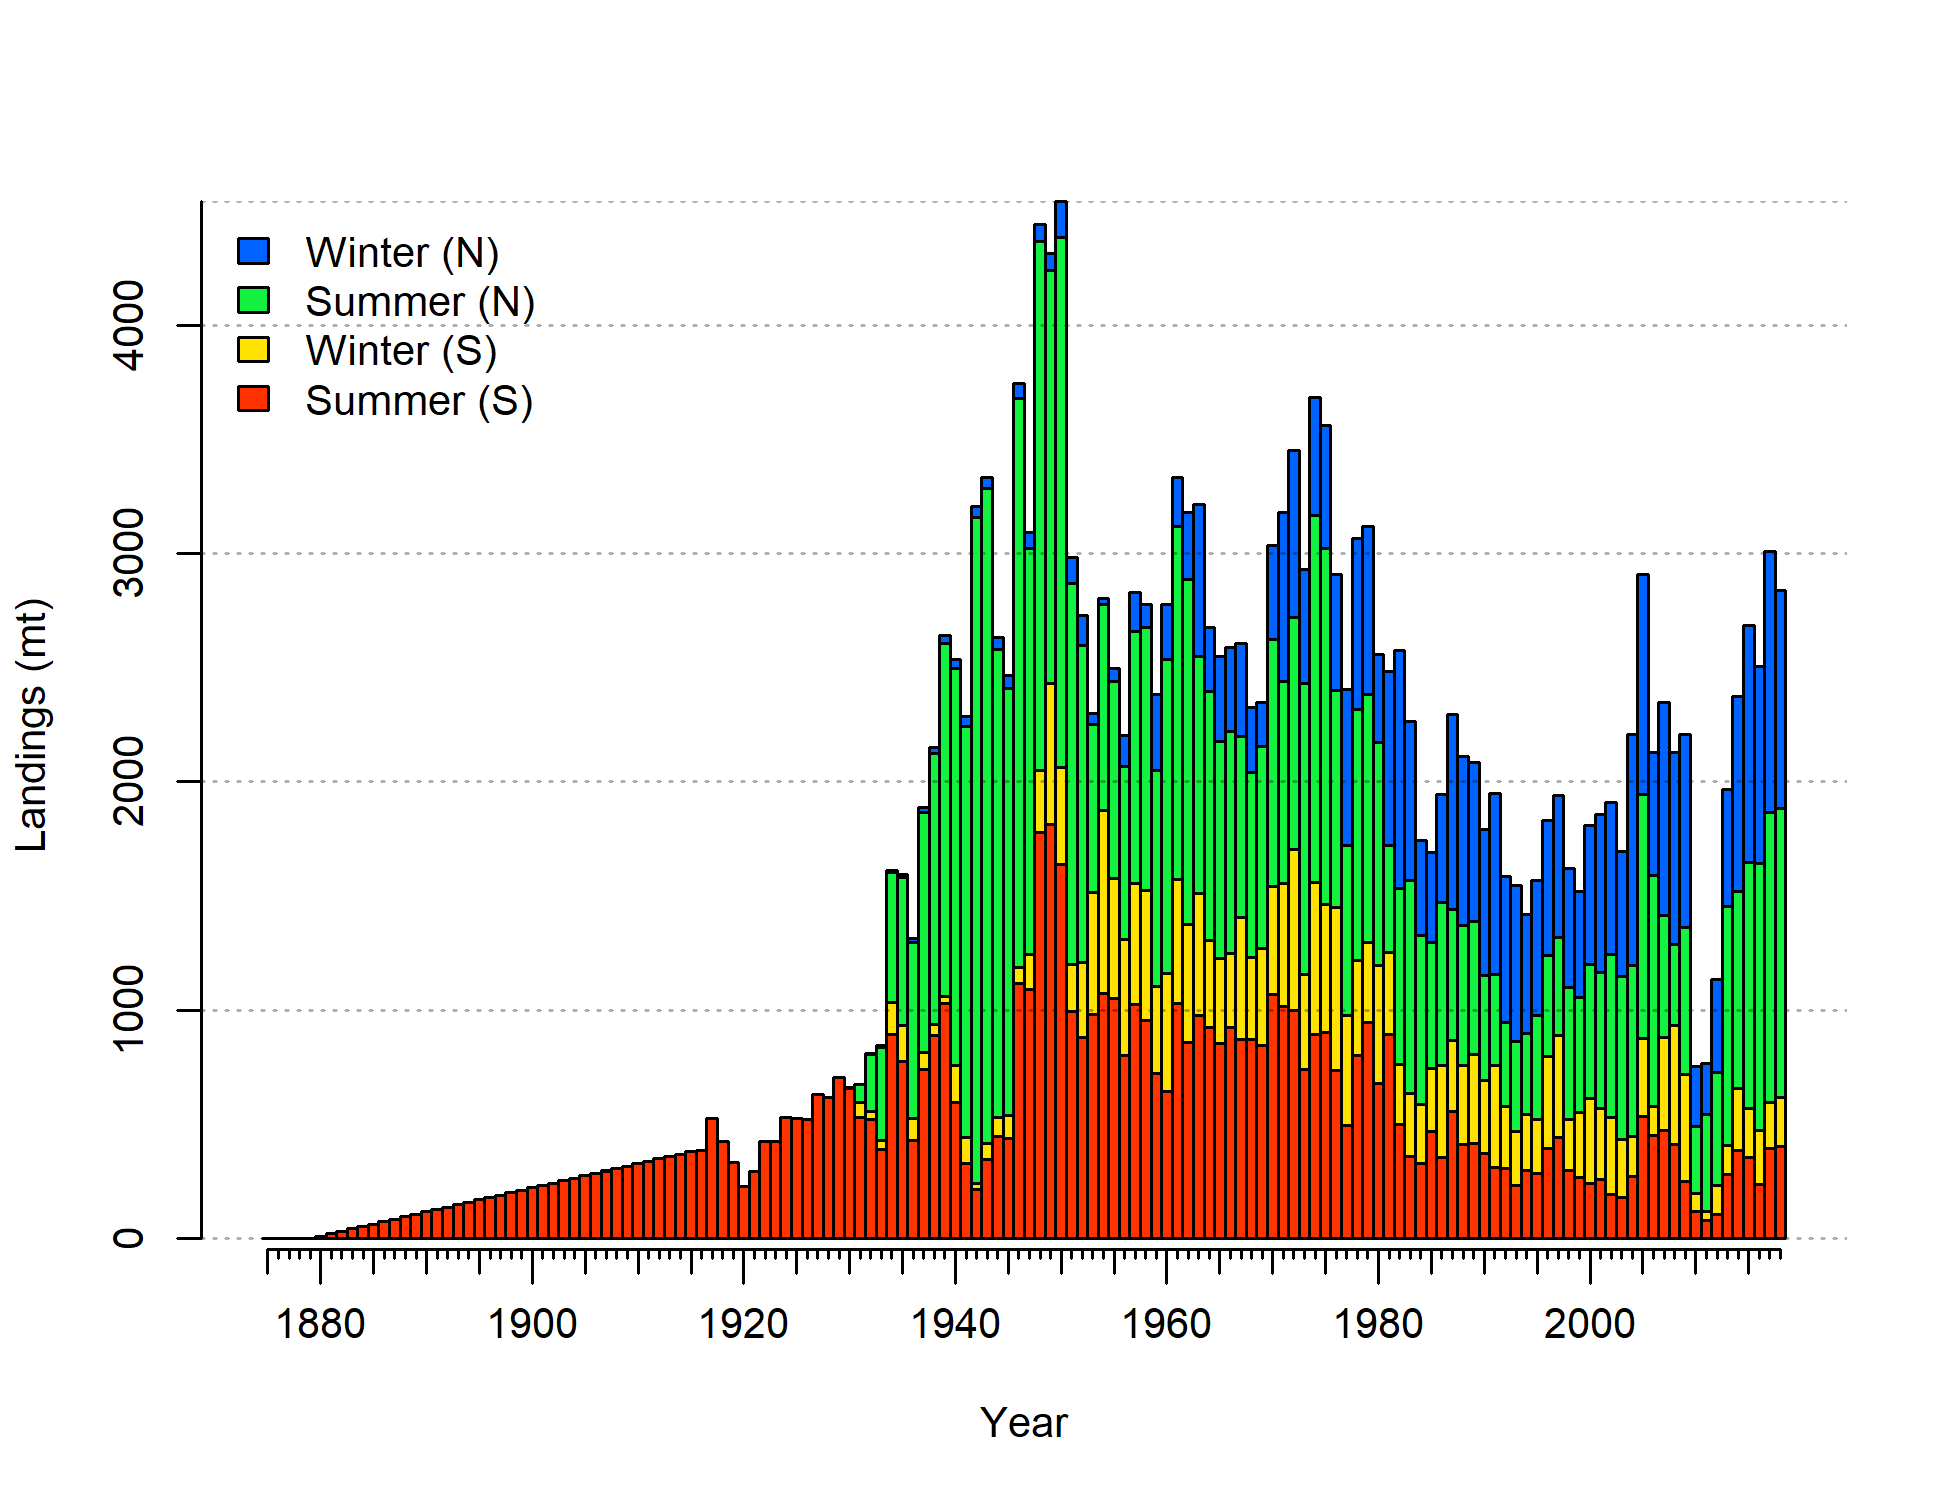
\includegraphics{r4ss/plots_mod1/catch2 landings stacked.png}
\caption{Total catches petrale sole. \label{fig:Catch}}
\end{figure}

\FloatBarrier

\begin{figure}
\centering
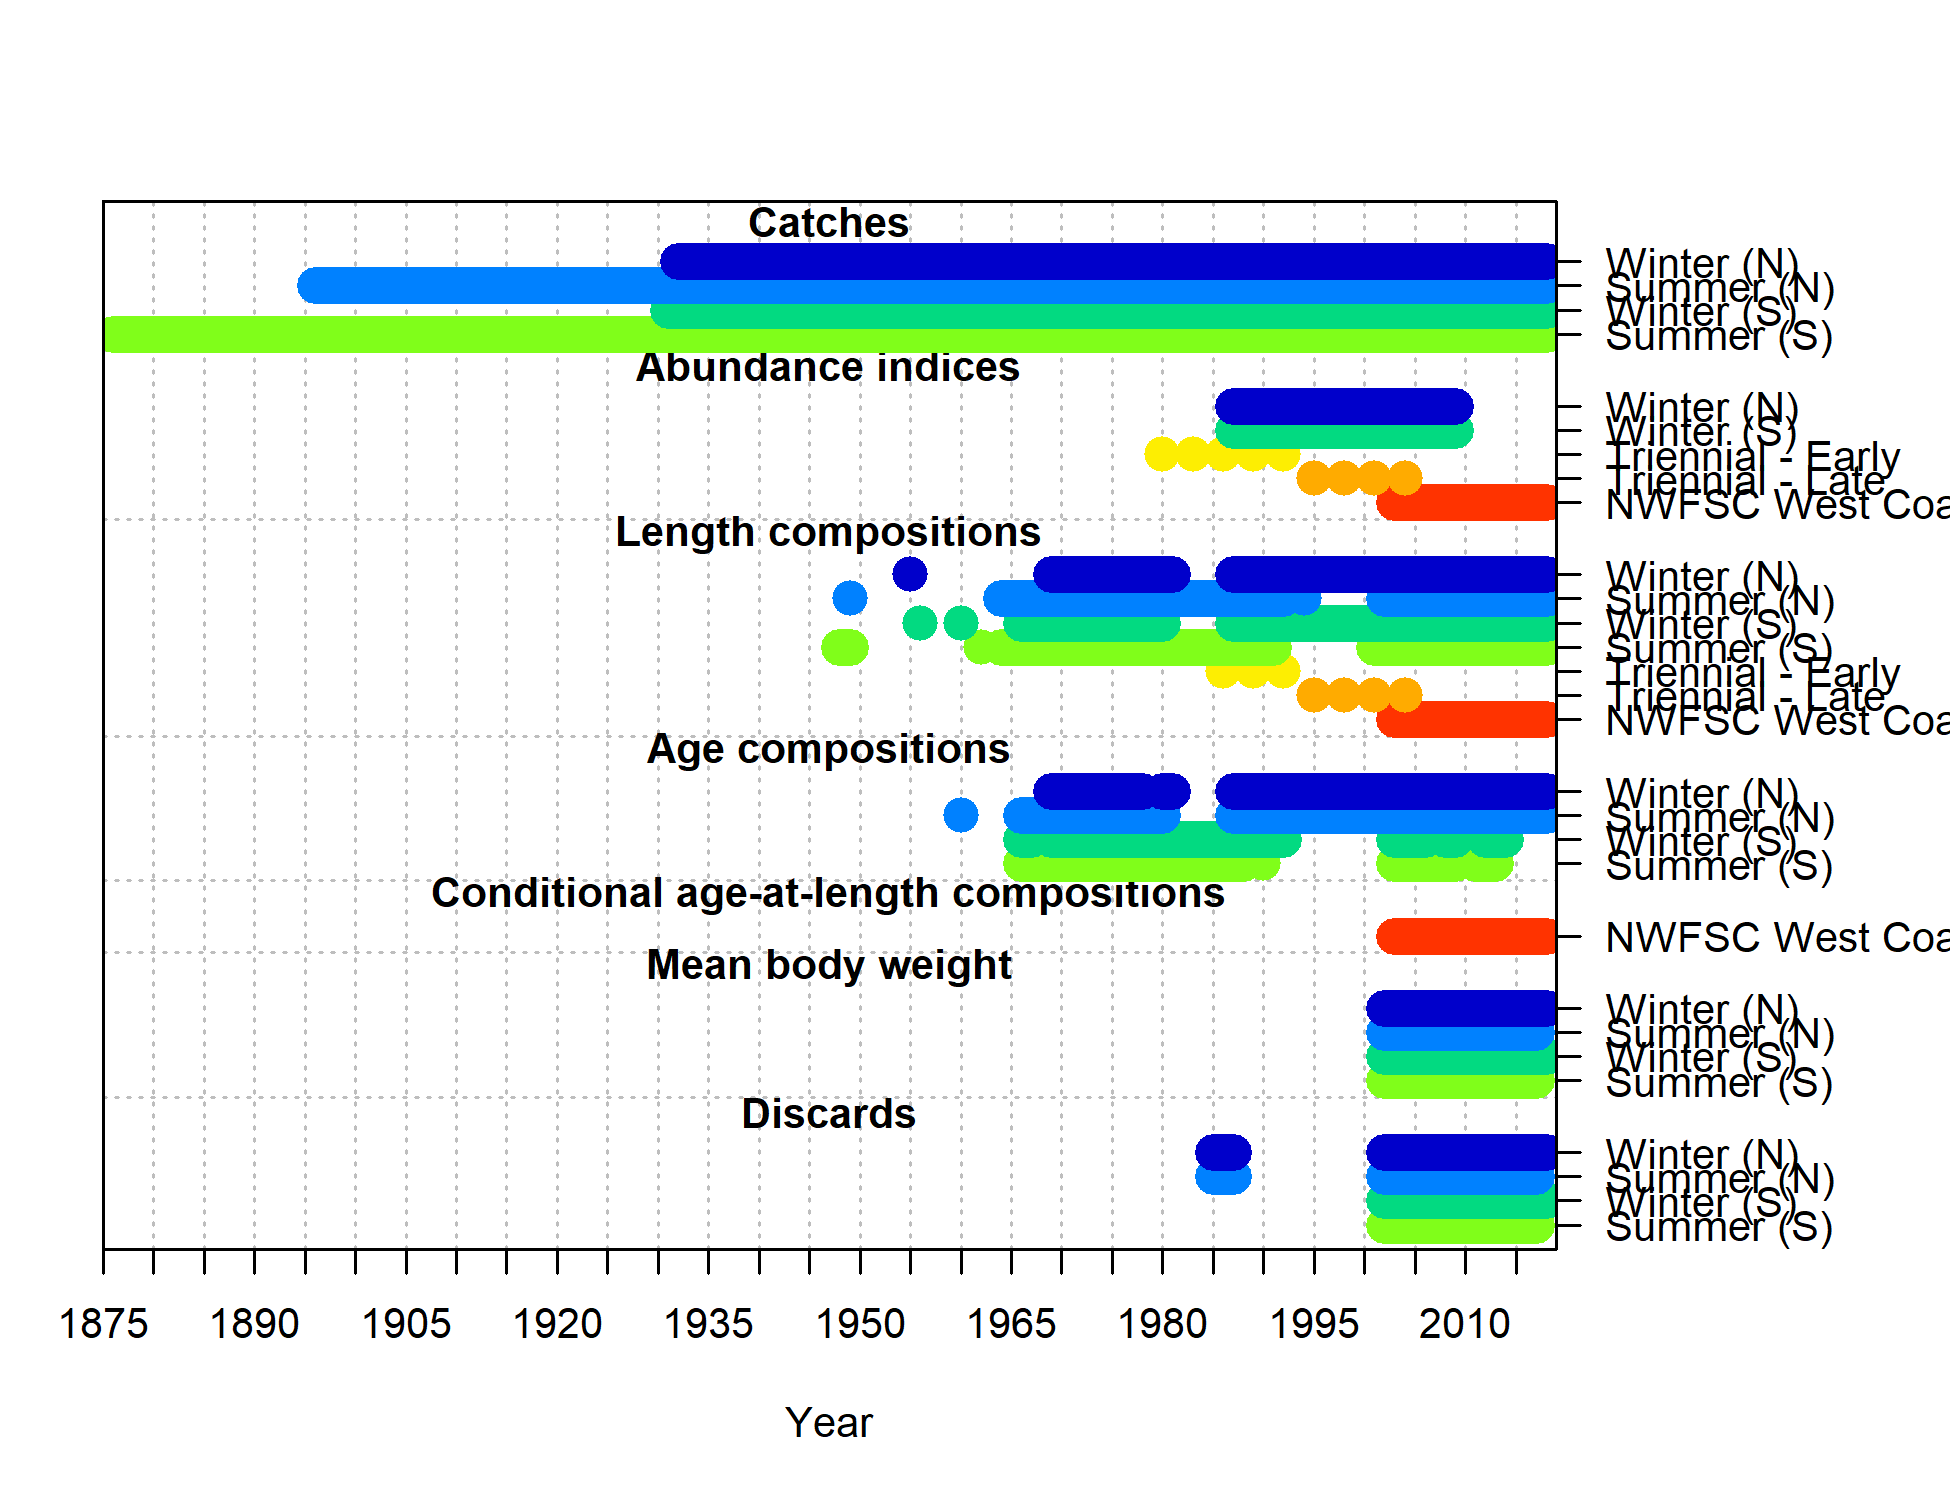
\includegraphics{r4ss/plots_mod1/data_plot.png}
\caption{Summary of data sources used in the base model.
\label{fig:data_plot}}
\end{figure}

\FloatBarrier

\begin{figure}
\centering
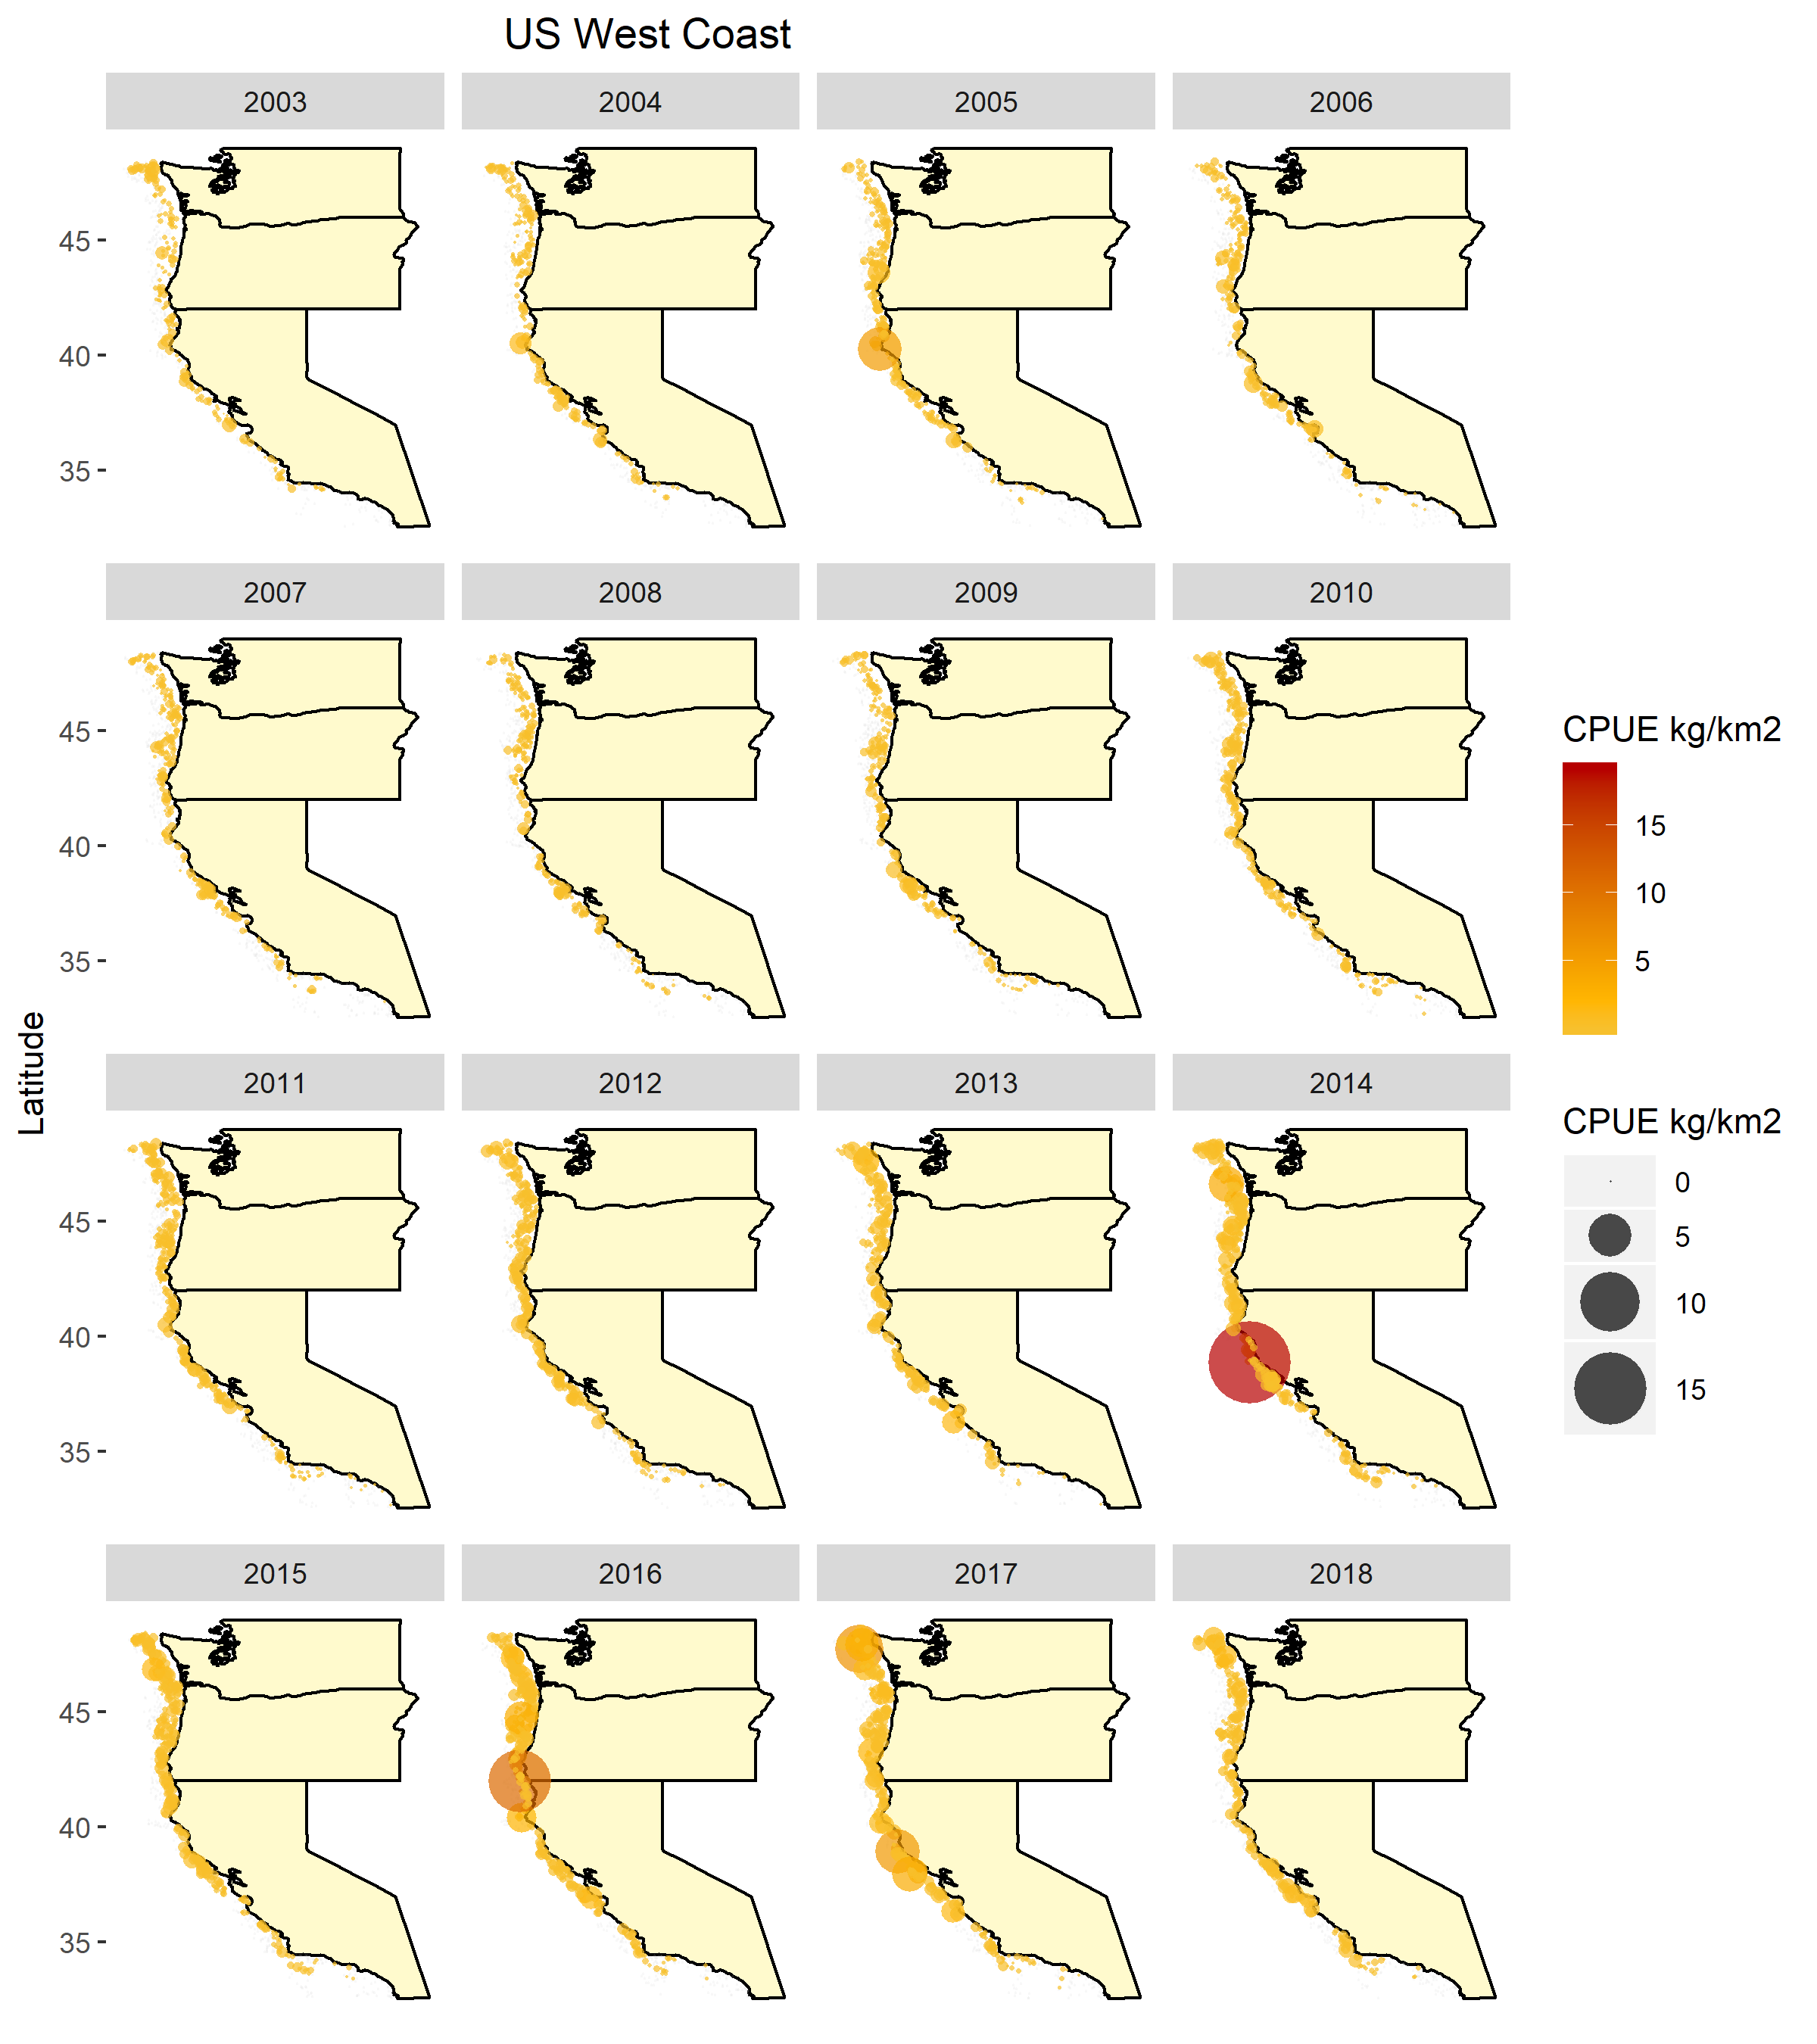
\includegraphics{Figures/NWFSC_CPUE_Map_Year.png}
\caption{Map of the catch-per-unit-effort across by year for the NWFSC
West Coast Groundfish Bottom Trawl Survey data. \label{fig:nw_map}}
\end{figure}

\FloatBarrier

\begin{figure}
\centering
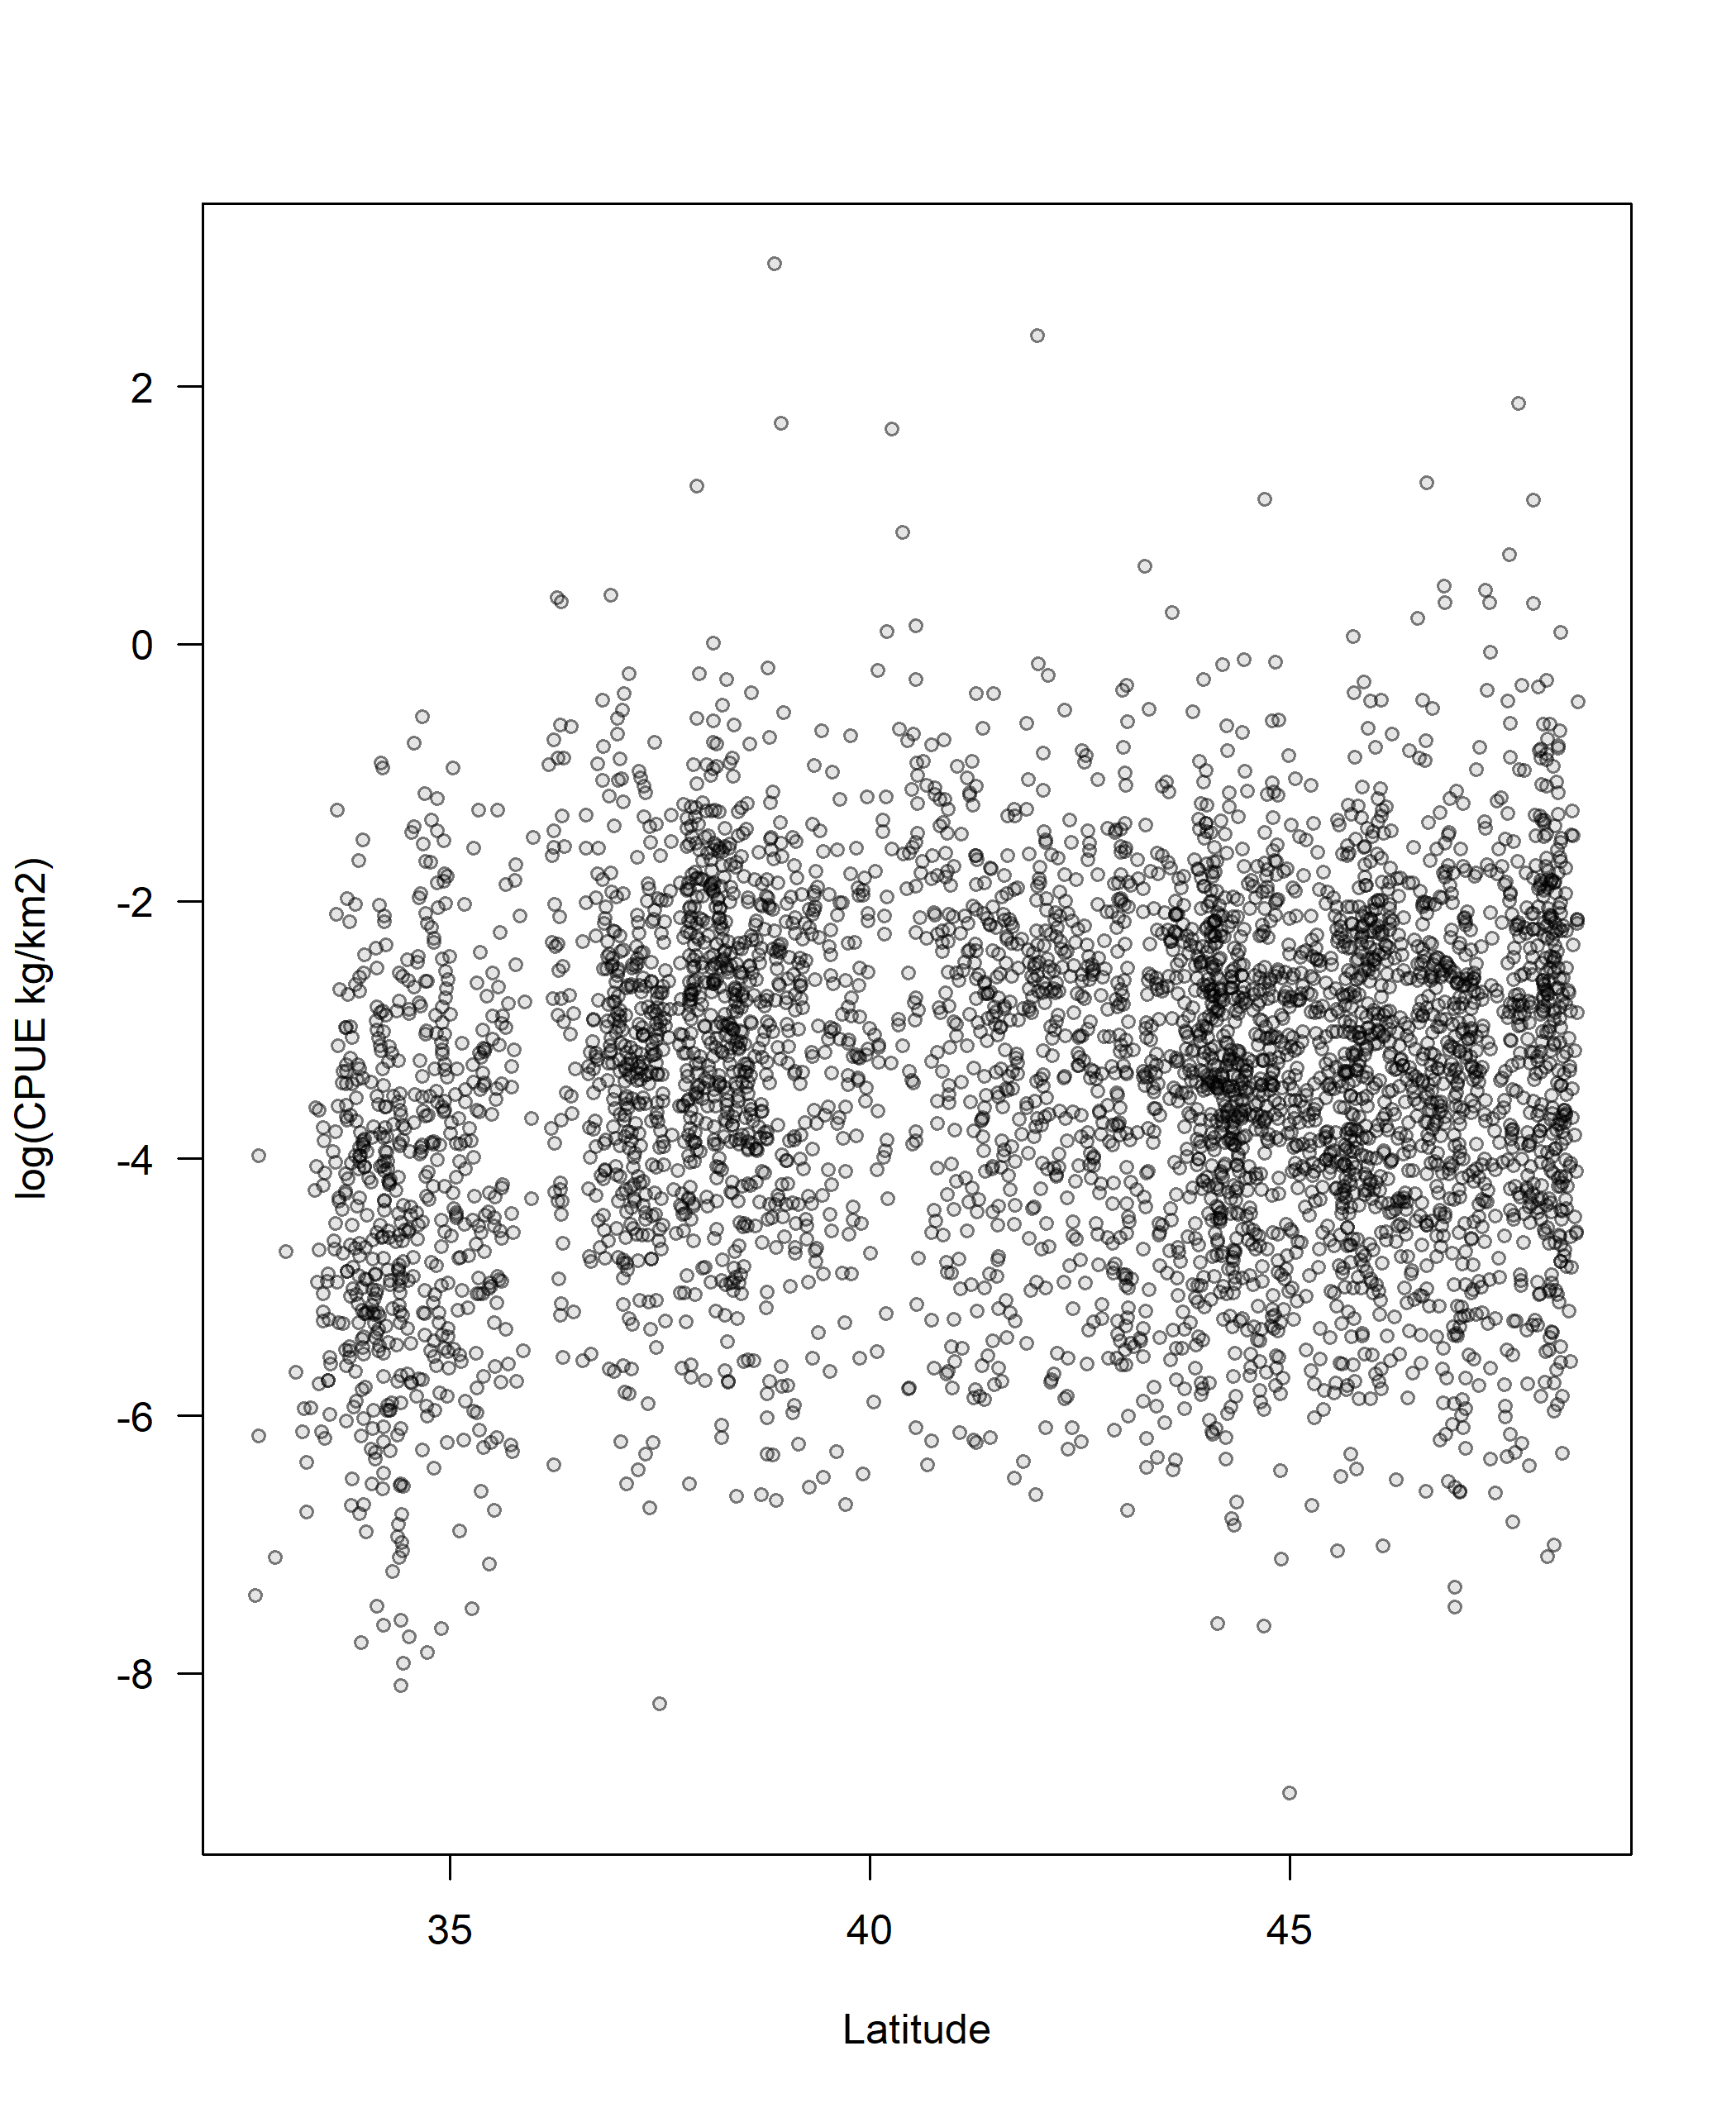
\includegraphics{Figures/NWFSC_CPUE_Lat.png}
\caption{Catch-per-unit-effort (in log space) by latitude for the NWFSC
West Coast Groundfish Bottom Trawl Survey data. \label{fig:nw_cpue_lat}}
\end{figure}

\FloatBarrier

\begin{figure}
\centering
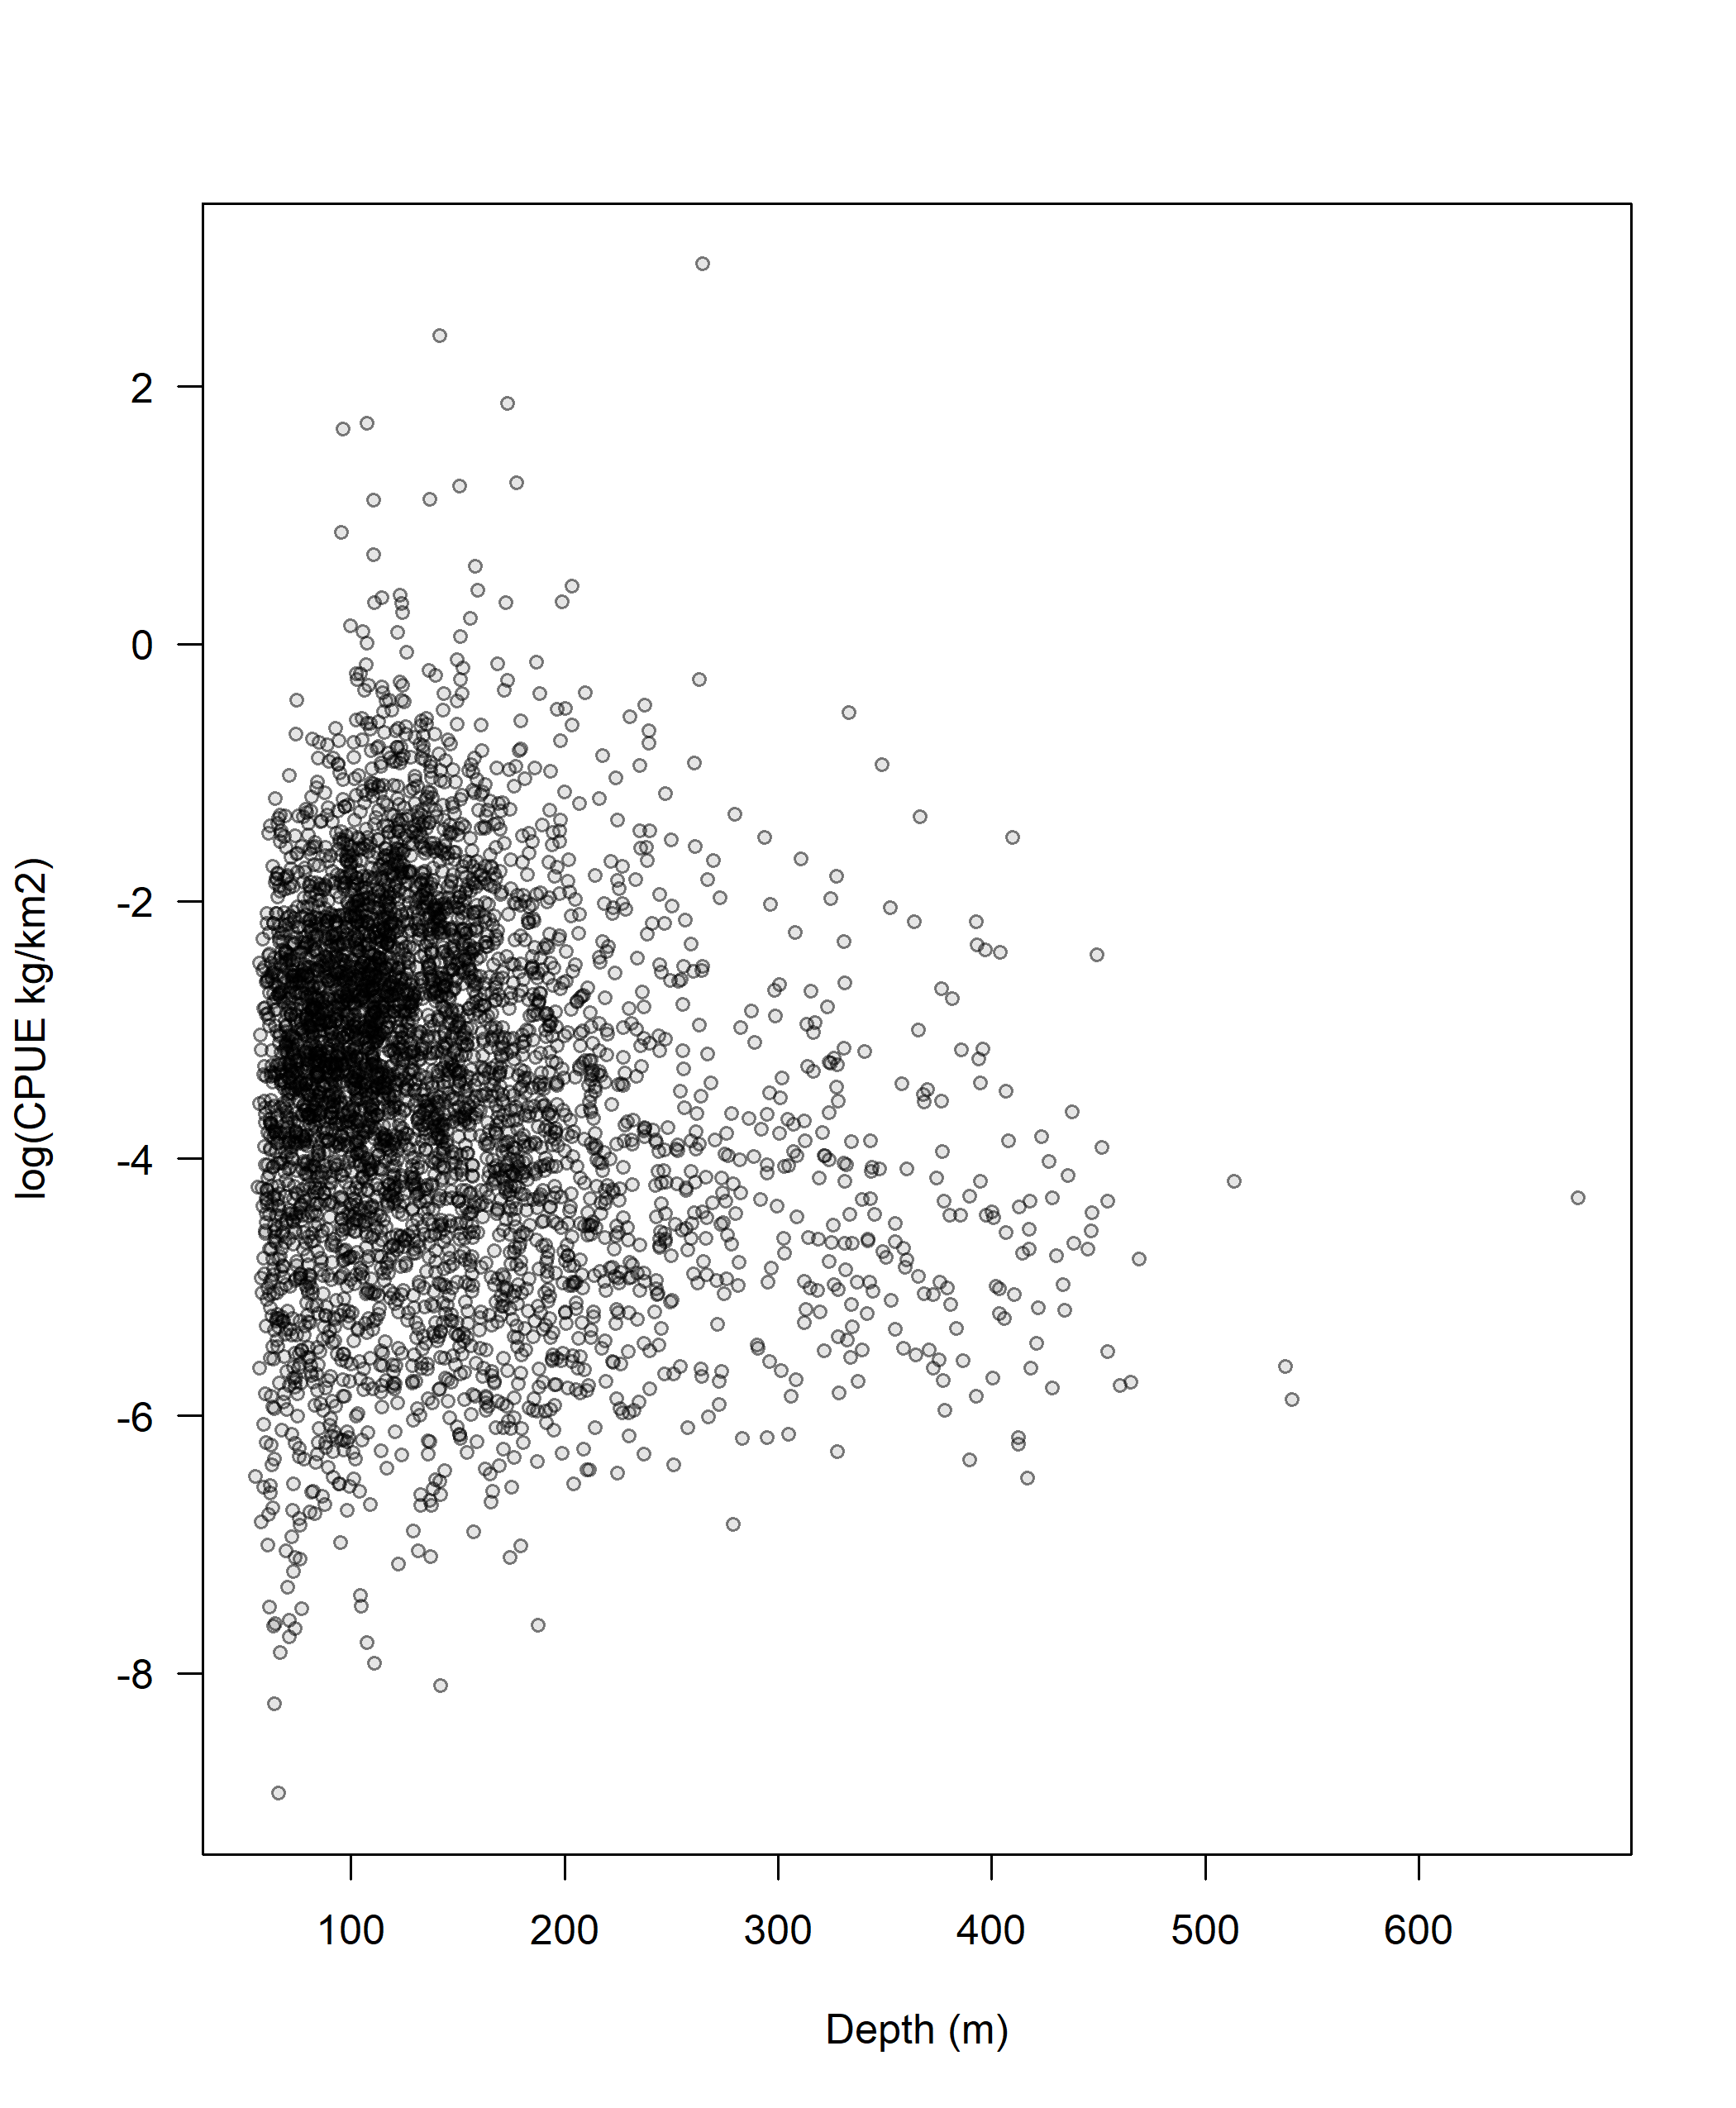
\includegraphics{Figures/NWFSC_CPUE_Depth.png}
\caption{Catch-per-unit-effort (in log space) by depth for the NWFSC
West Coast Groundfish Bottom Trawl Survey data.
\label{fig:nw_cpue_depth}}
\end{figure}

\FloatBarrier

\begin{figure}
\centering
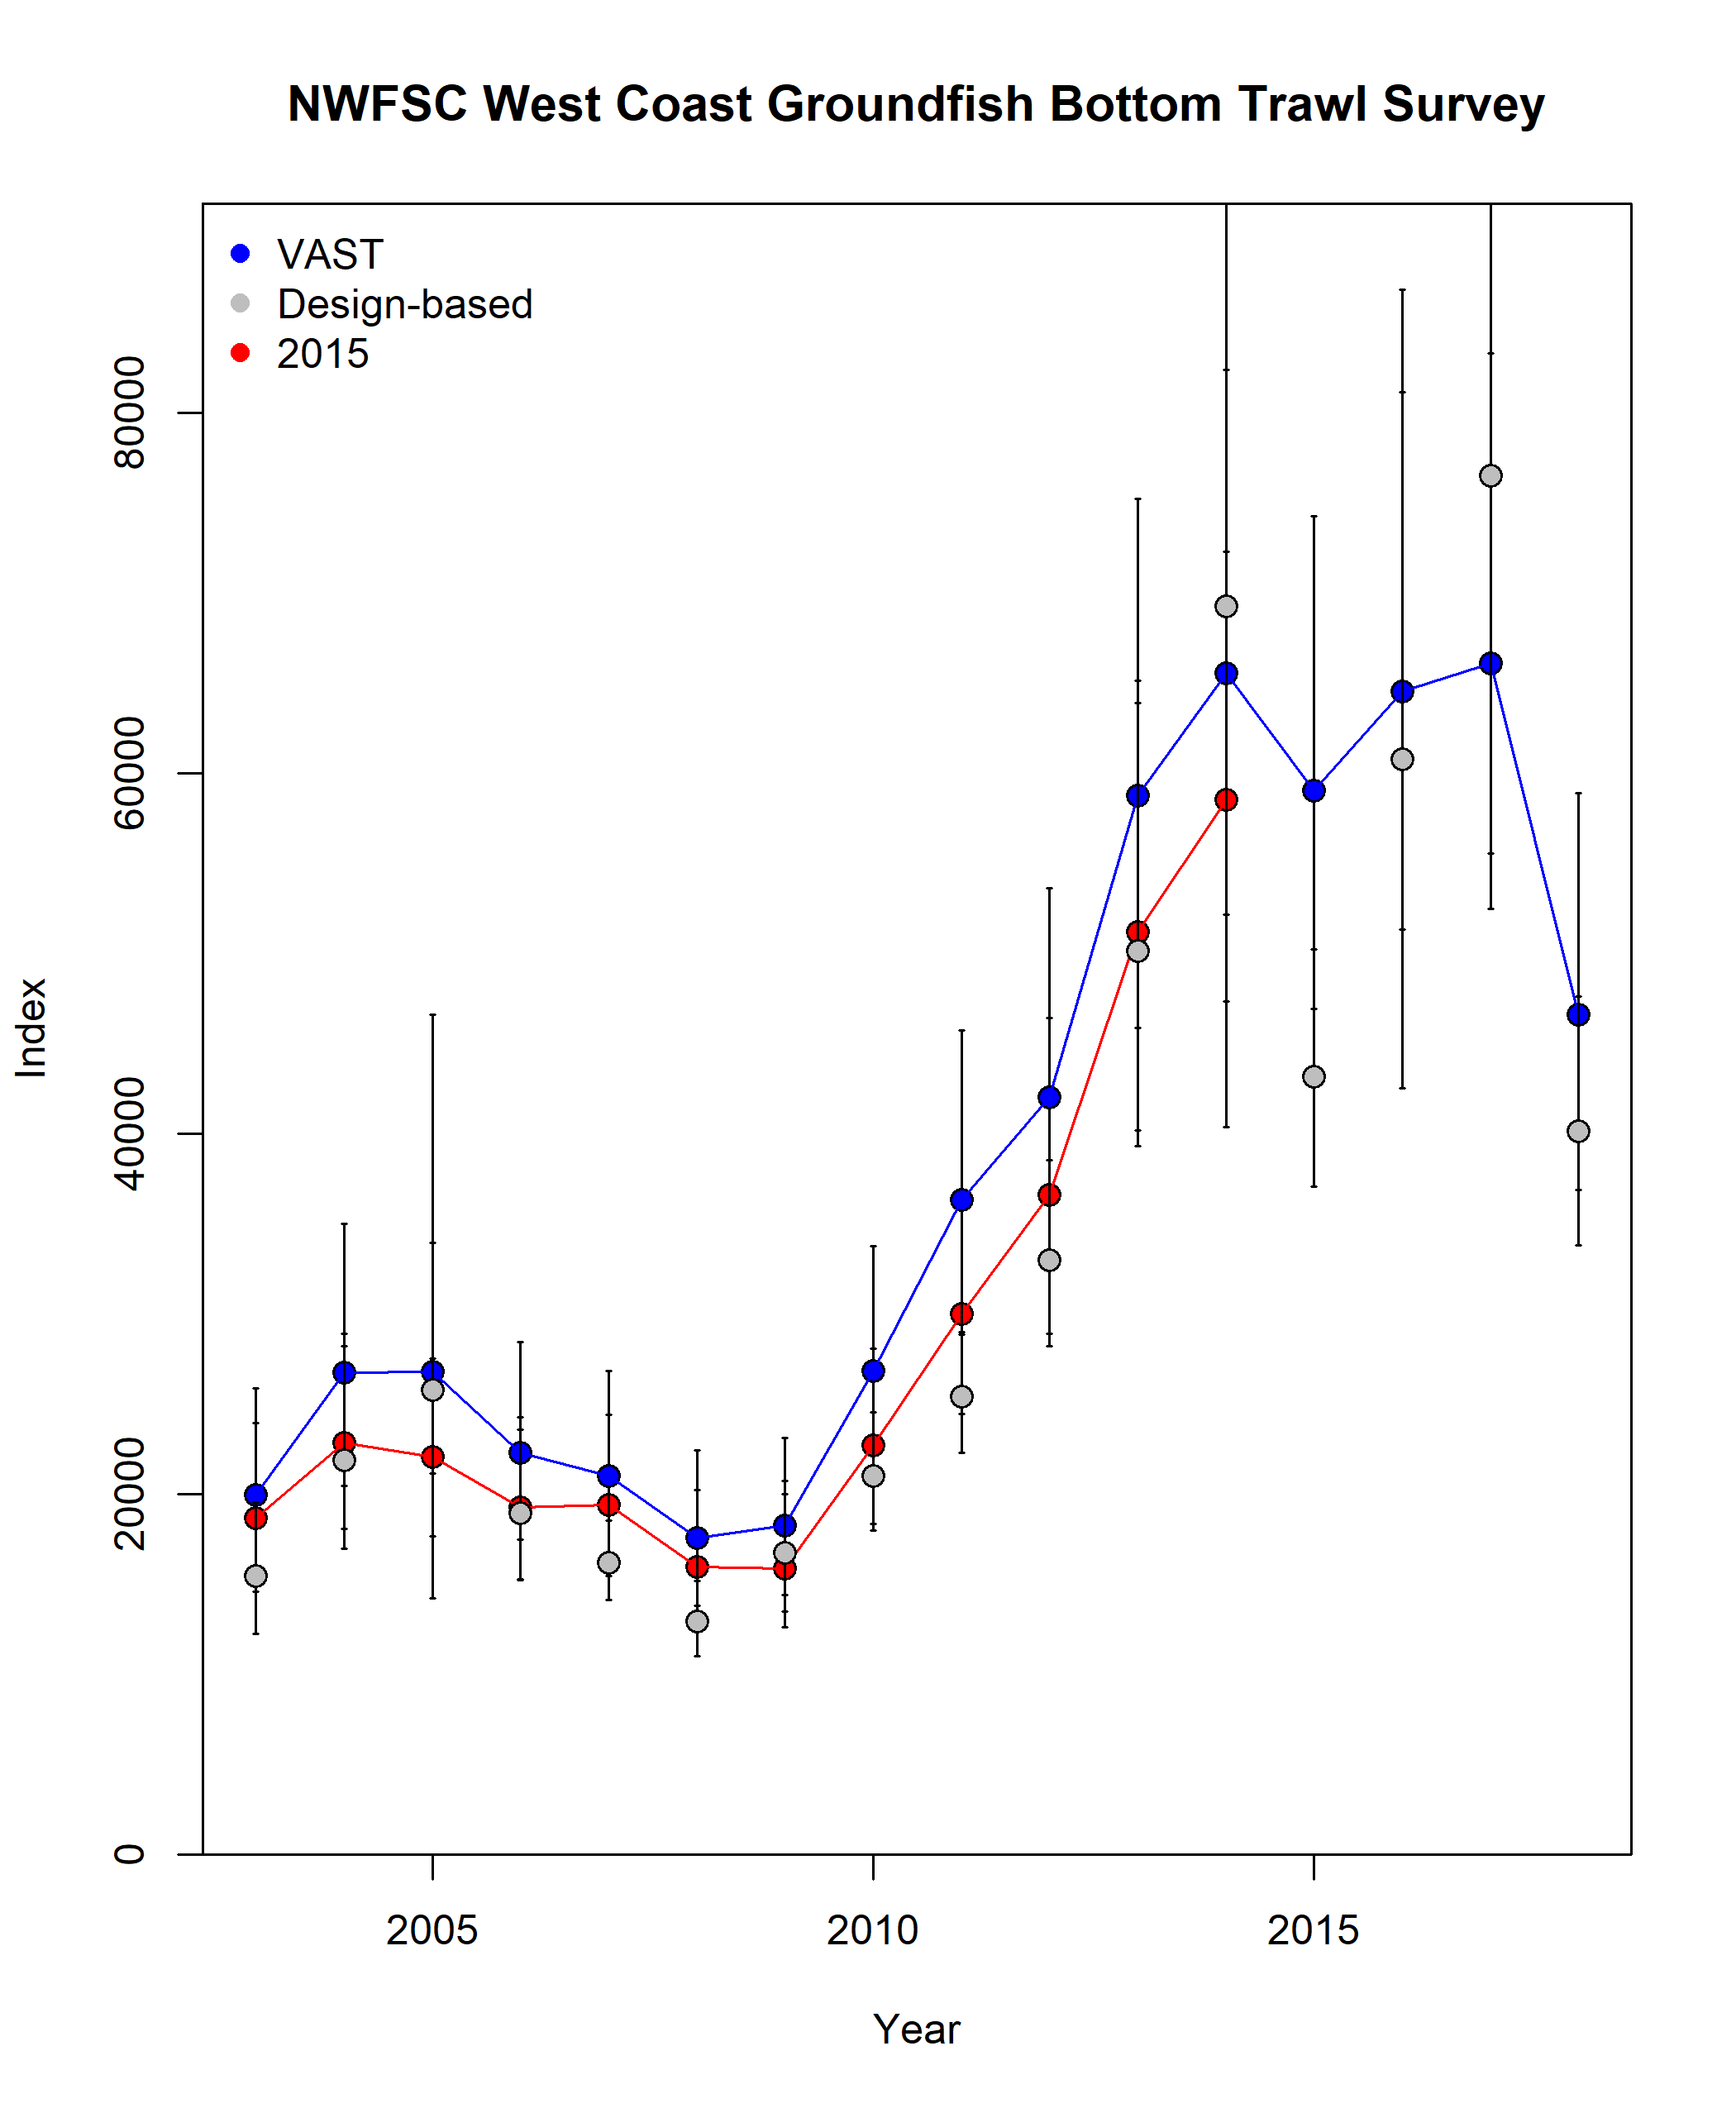
\includegraphics{Figures/NWFSC_Index.png}
\caption{Estimated index of abundance from the NWFSC West Coast
Groundfish Bottom Trawl Survey data compared to the design-based index
and the index from the 2015 update assessment. \label{fig:nw_index}}
\end{figure}

\FloatBarrier

\begin{figure}
\centering
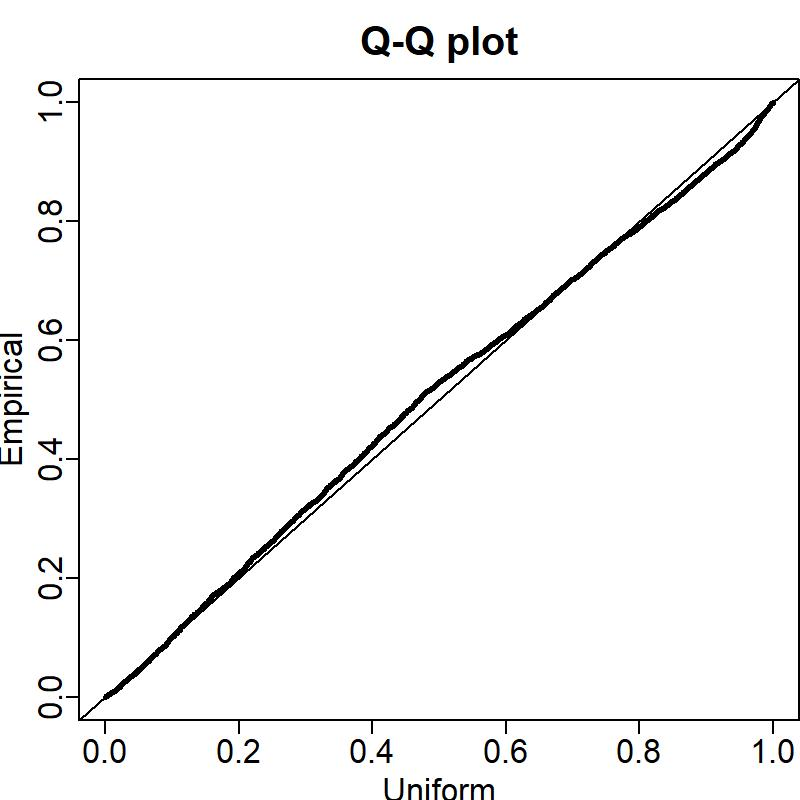
\includegraphics{Figures/nwfsc_Posterior_Predictive-Histogram-1.jpg}
\caption{QQ plot for the NWFSC West Coast Groundfish Bottom Trawl Survey
data. \label{fig:nw_qq}}
\end{figure}

\FloatBarrier

\begin{figure}
\centering
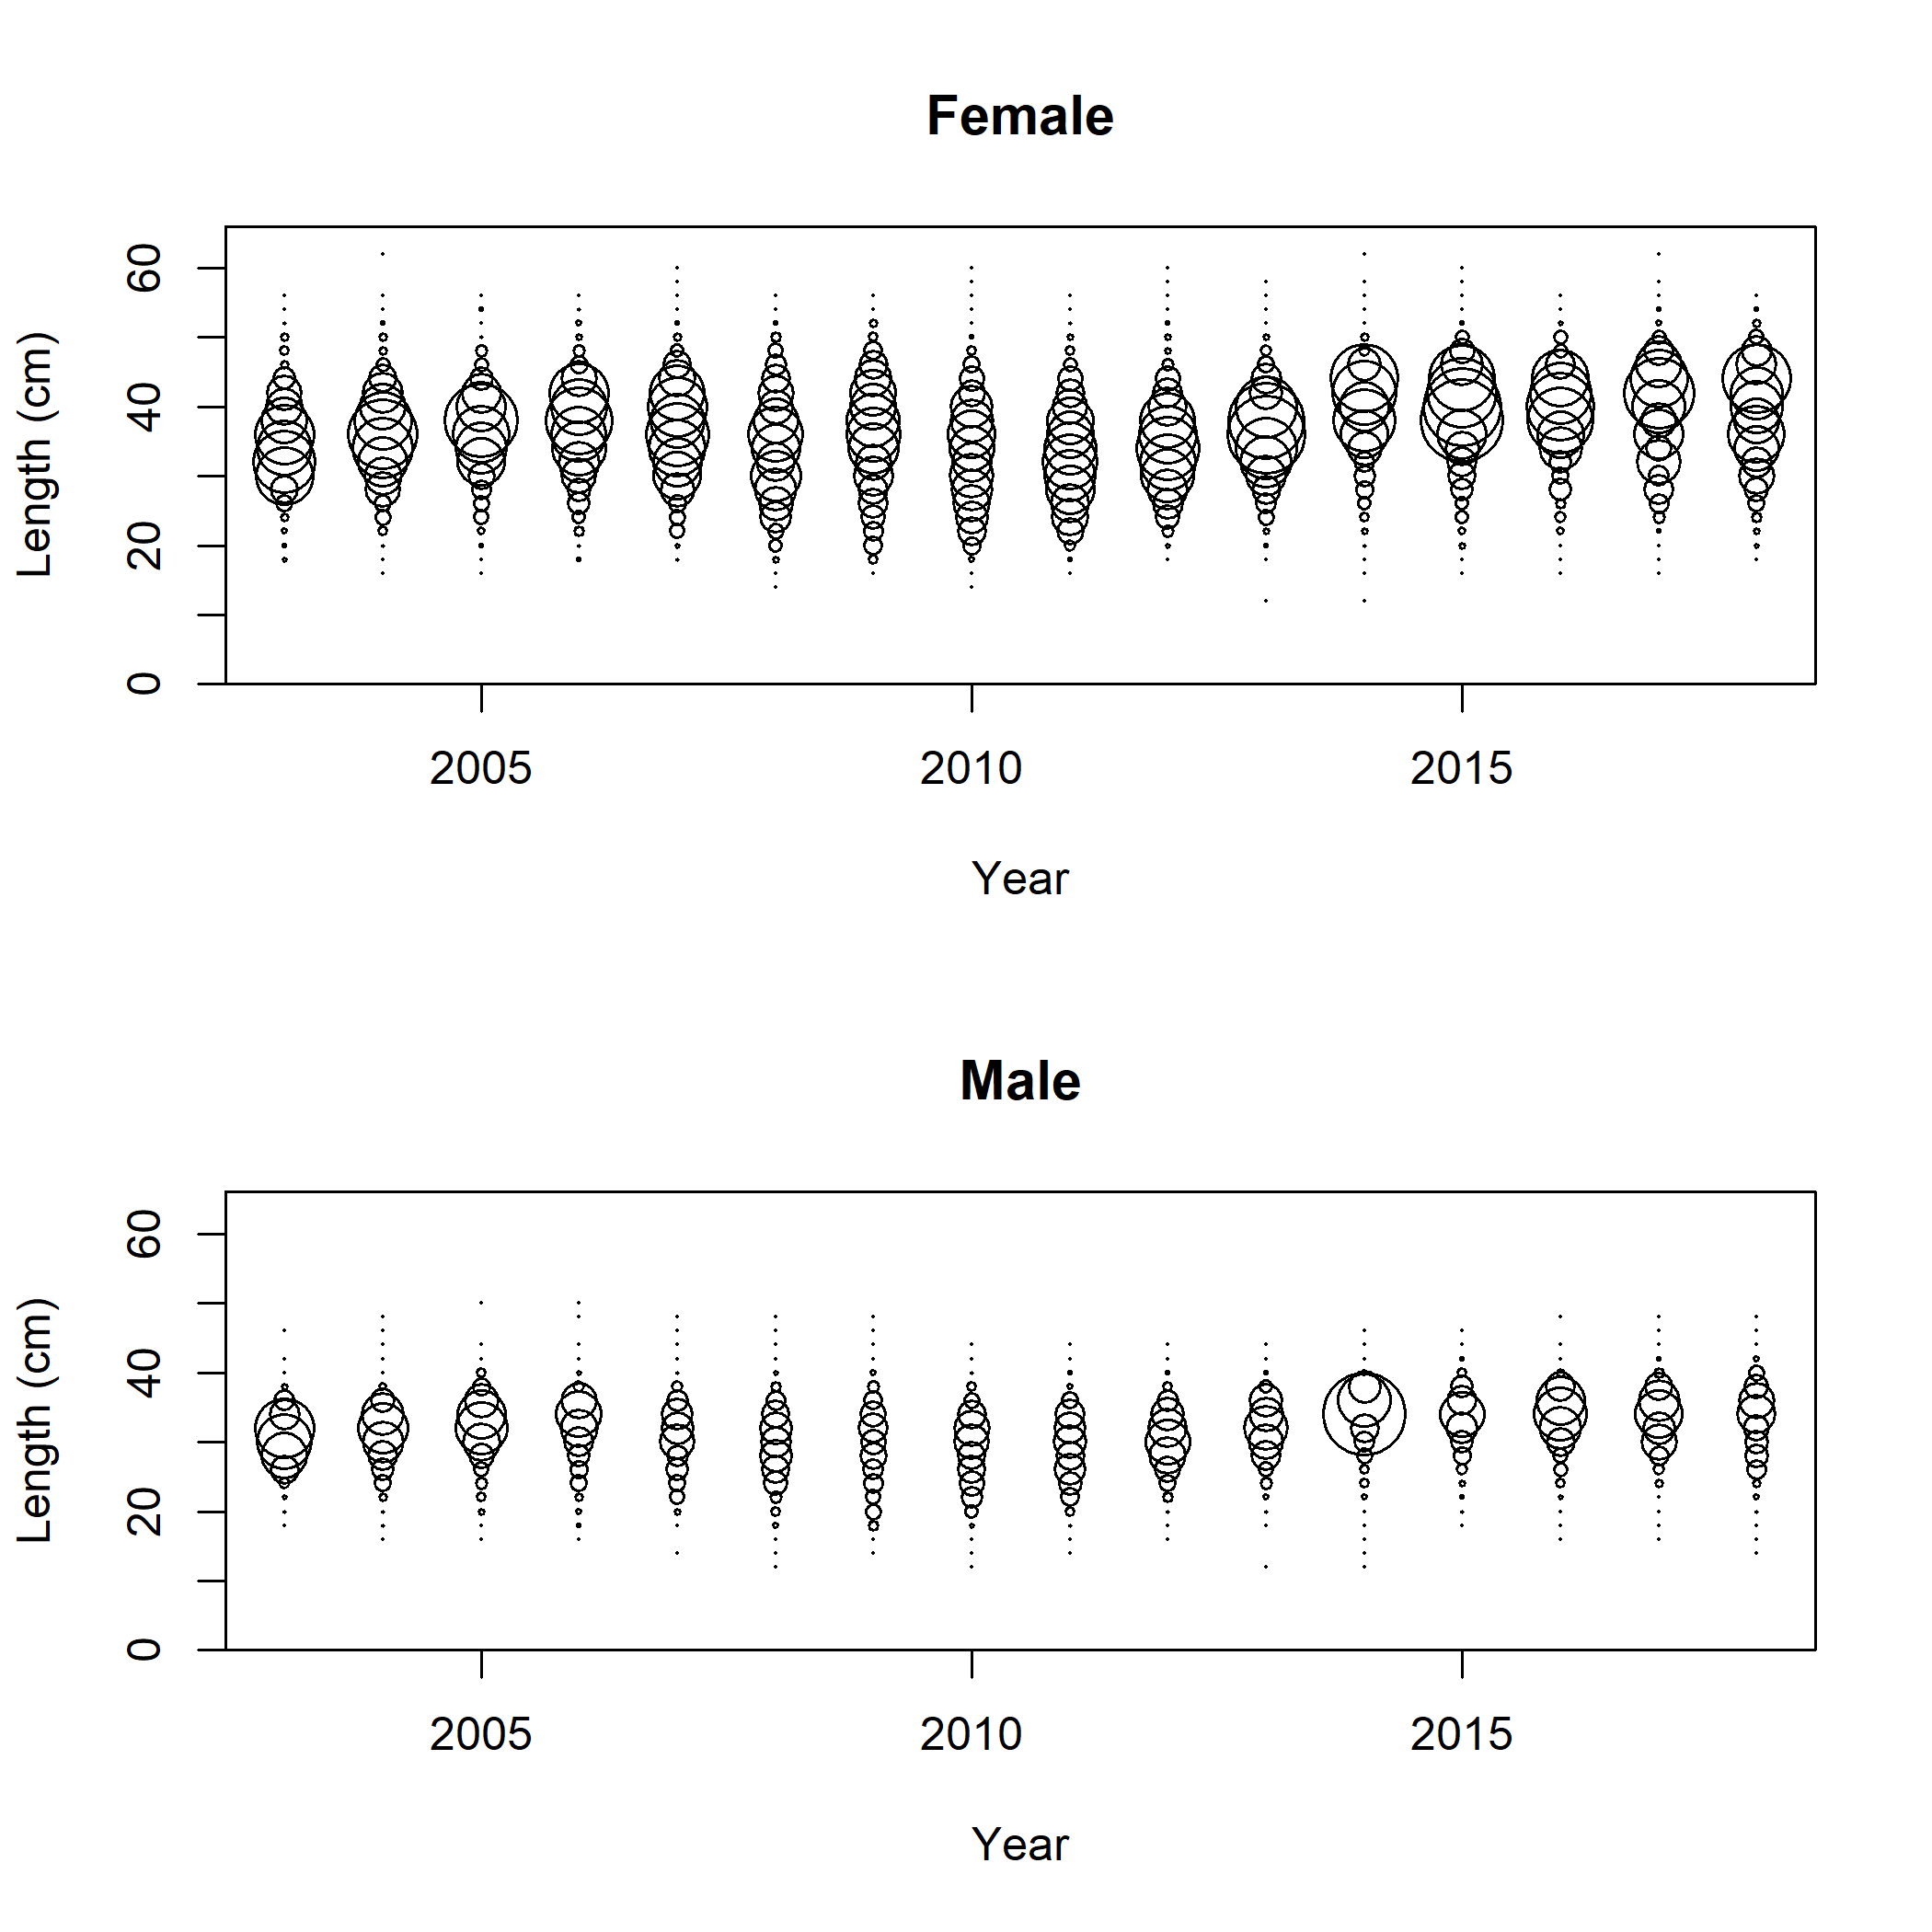
\includegraphics{Figures/NWFSC Groundfish Bottom Trawl Survey_Length_Frequency.png}
\caption{Length frequency by sex for the NWFSC West Coast Groundfish
Bottom Trawl Survey data. \label{fig:nw_len_freq}}
\end{figure}

\FloatBarrier

\begin{figure}
\centering
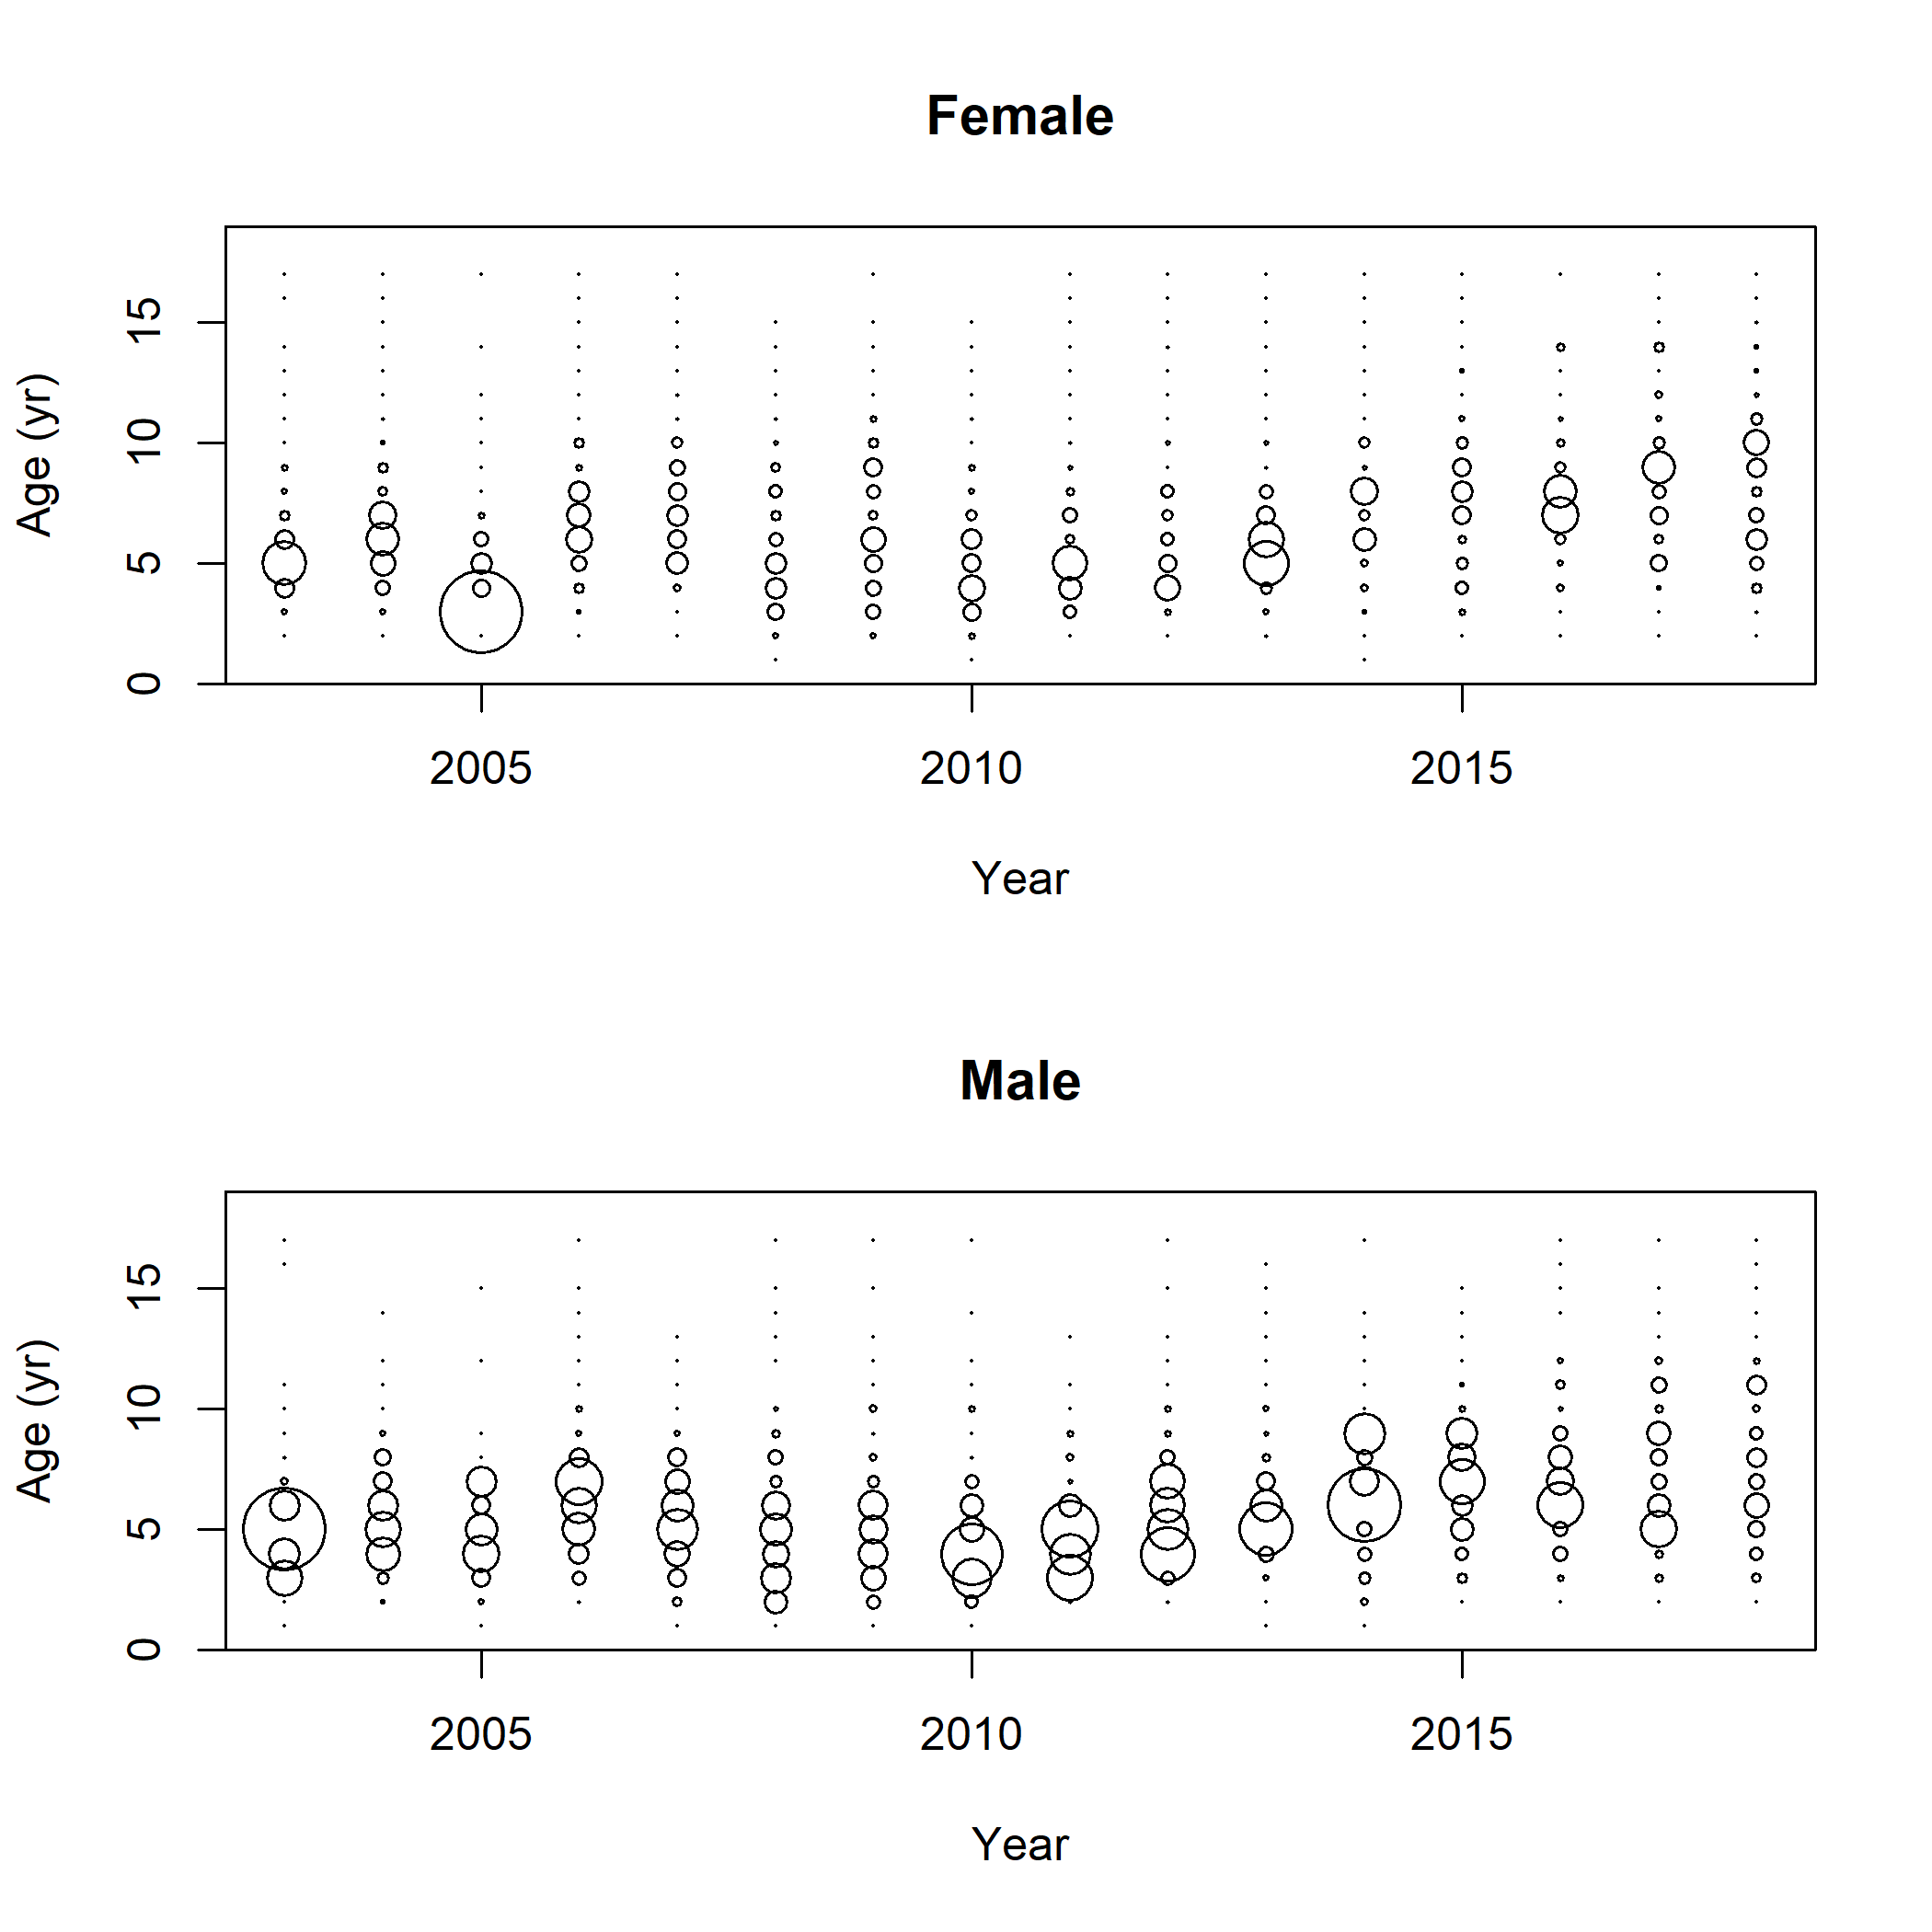
\includegraphics{Figures/NWFSC Groundfish Bottom Trawl Survey_Age_Frequency.png}
\caption{Age frequency by sex for the NWFSC West Coast Groundfish Bottom
Trawl Survey data. \label{fig:nw_age_freq}}
\end{figure}

\FloatBarrier

\begin{figure}
\centering
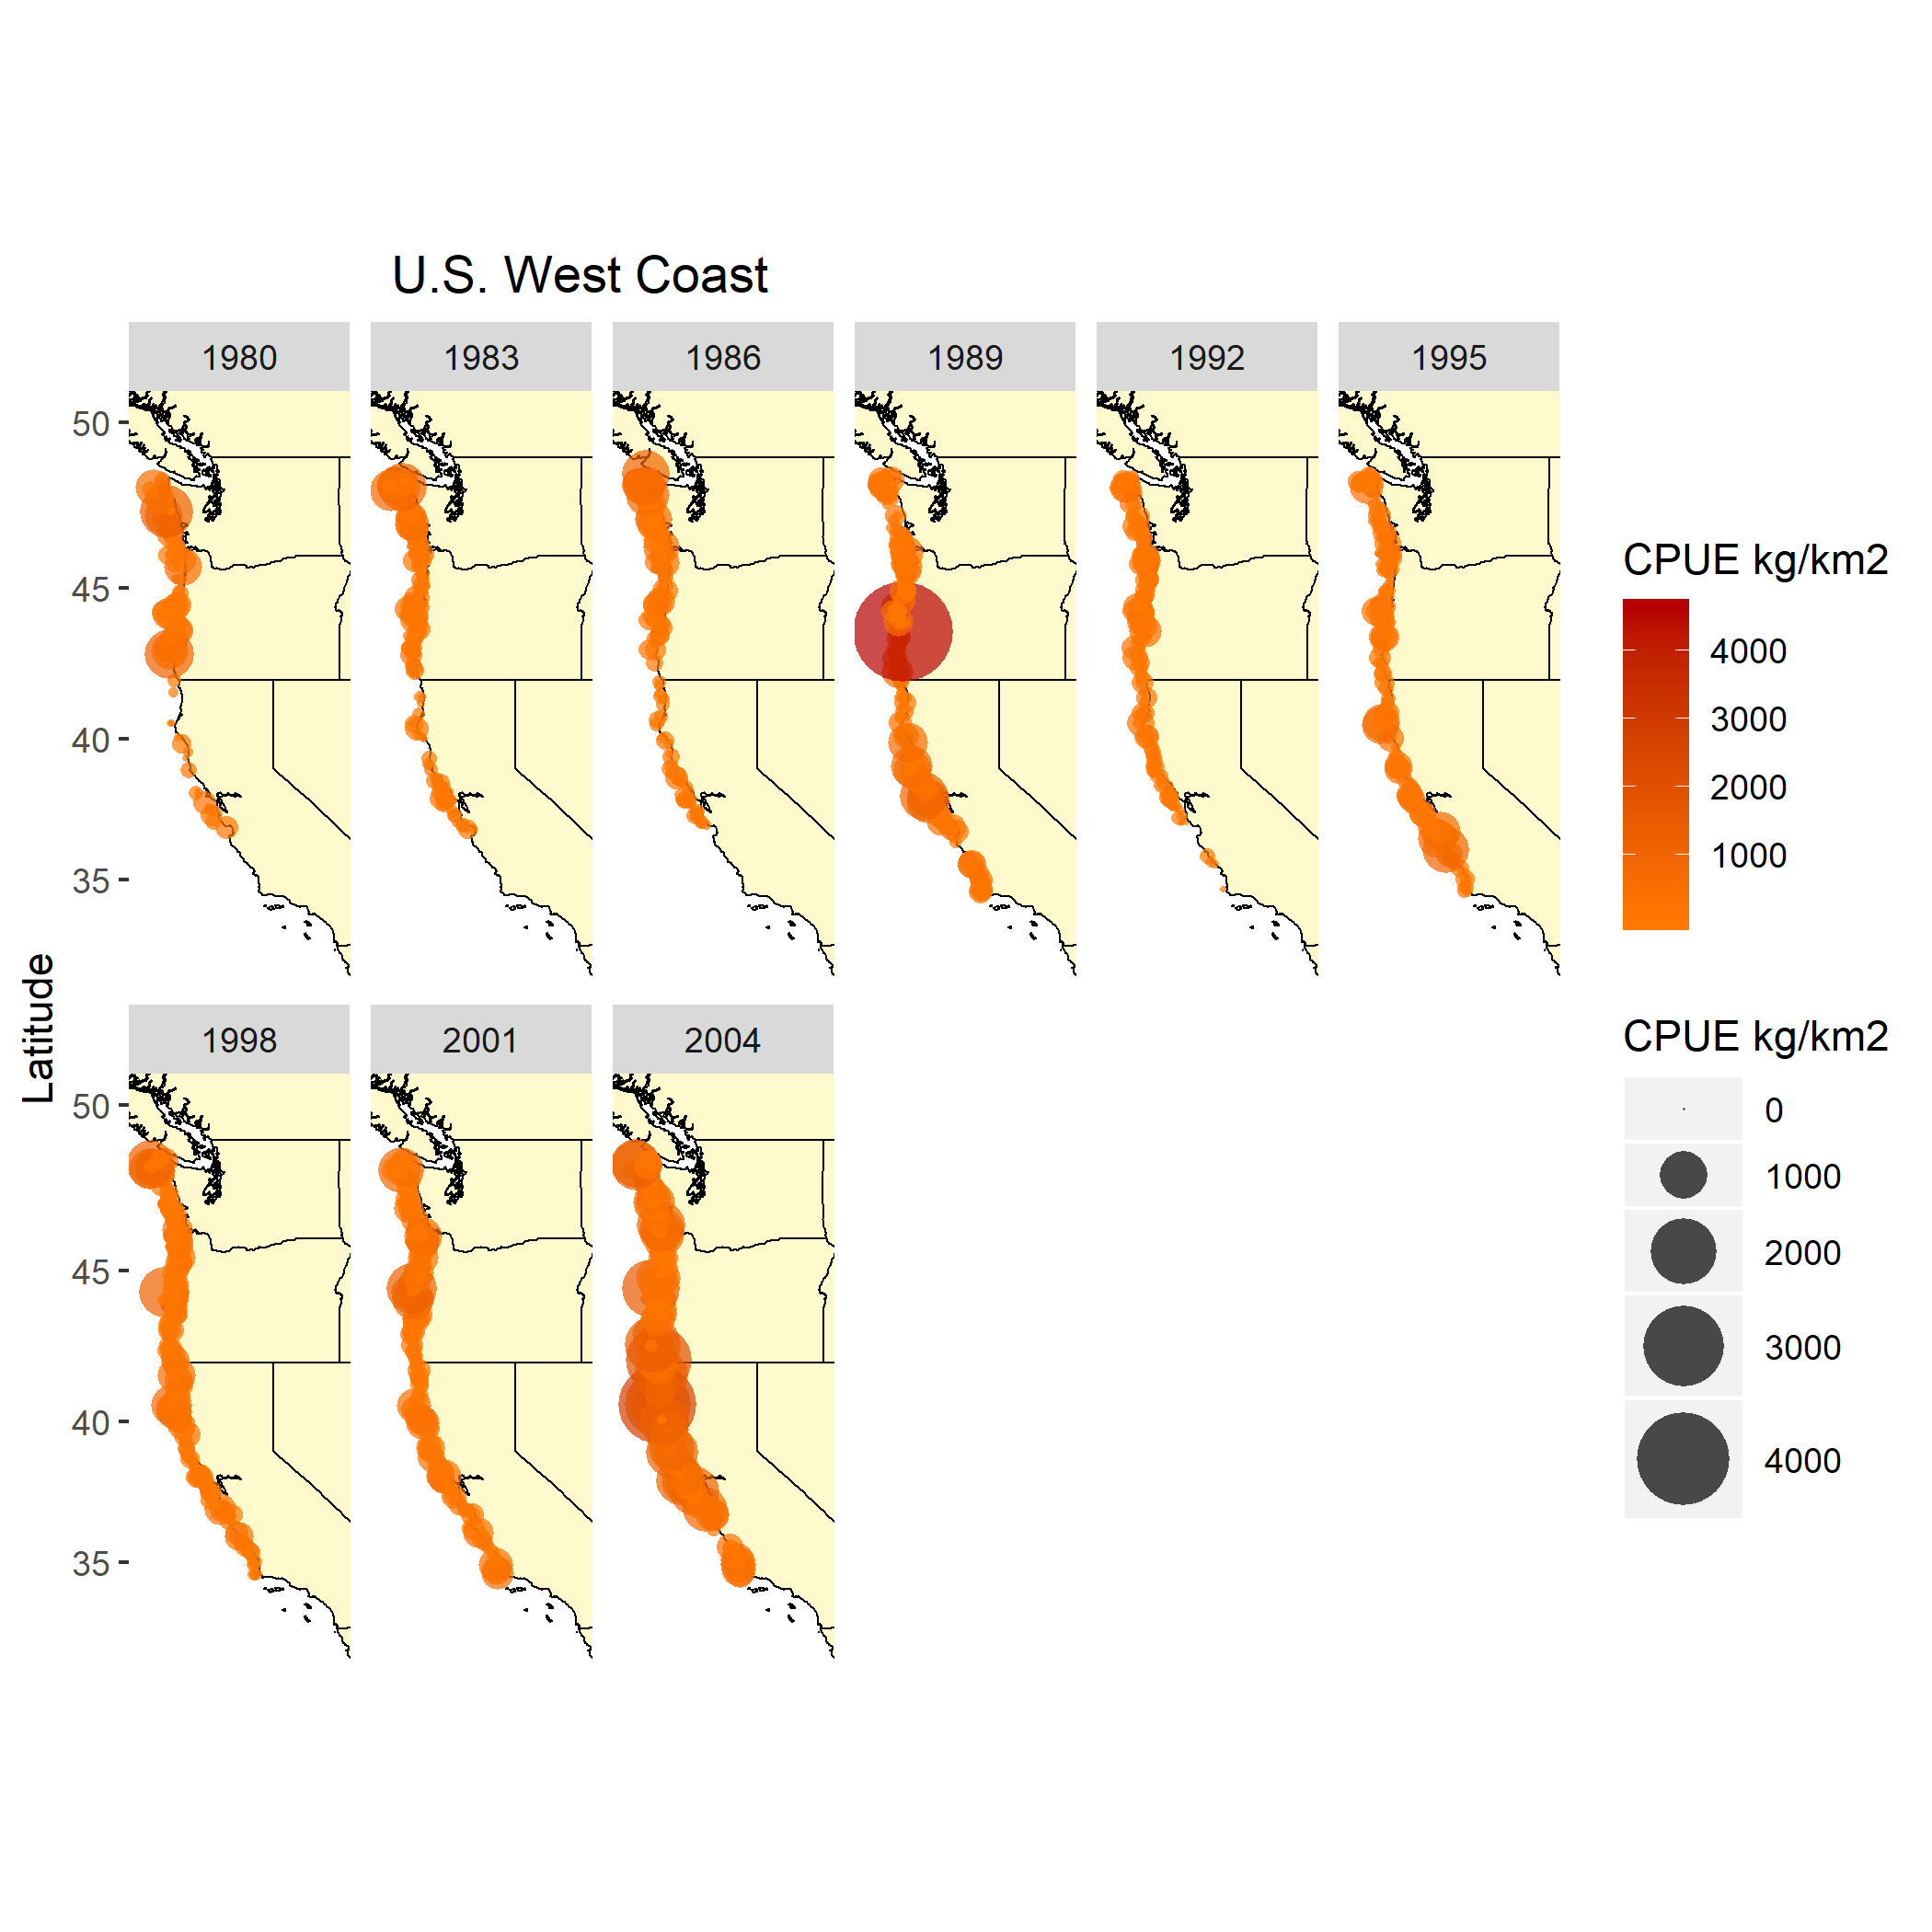
\includegraphics{Figures/Triennial_CPUE_Map_Year.png}
\caption{Map of the catch-per-unit-effort across by year for the
Triennial Survey data. \label{fig:tri_map}}
\end{figure}

\FloatBarrier

\begin{figure}
\centering
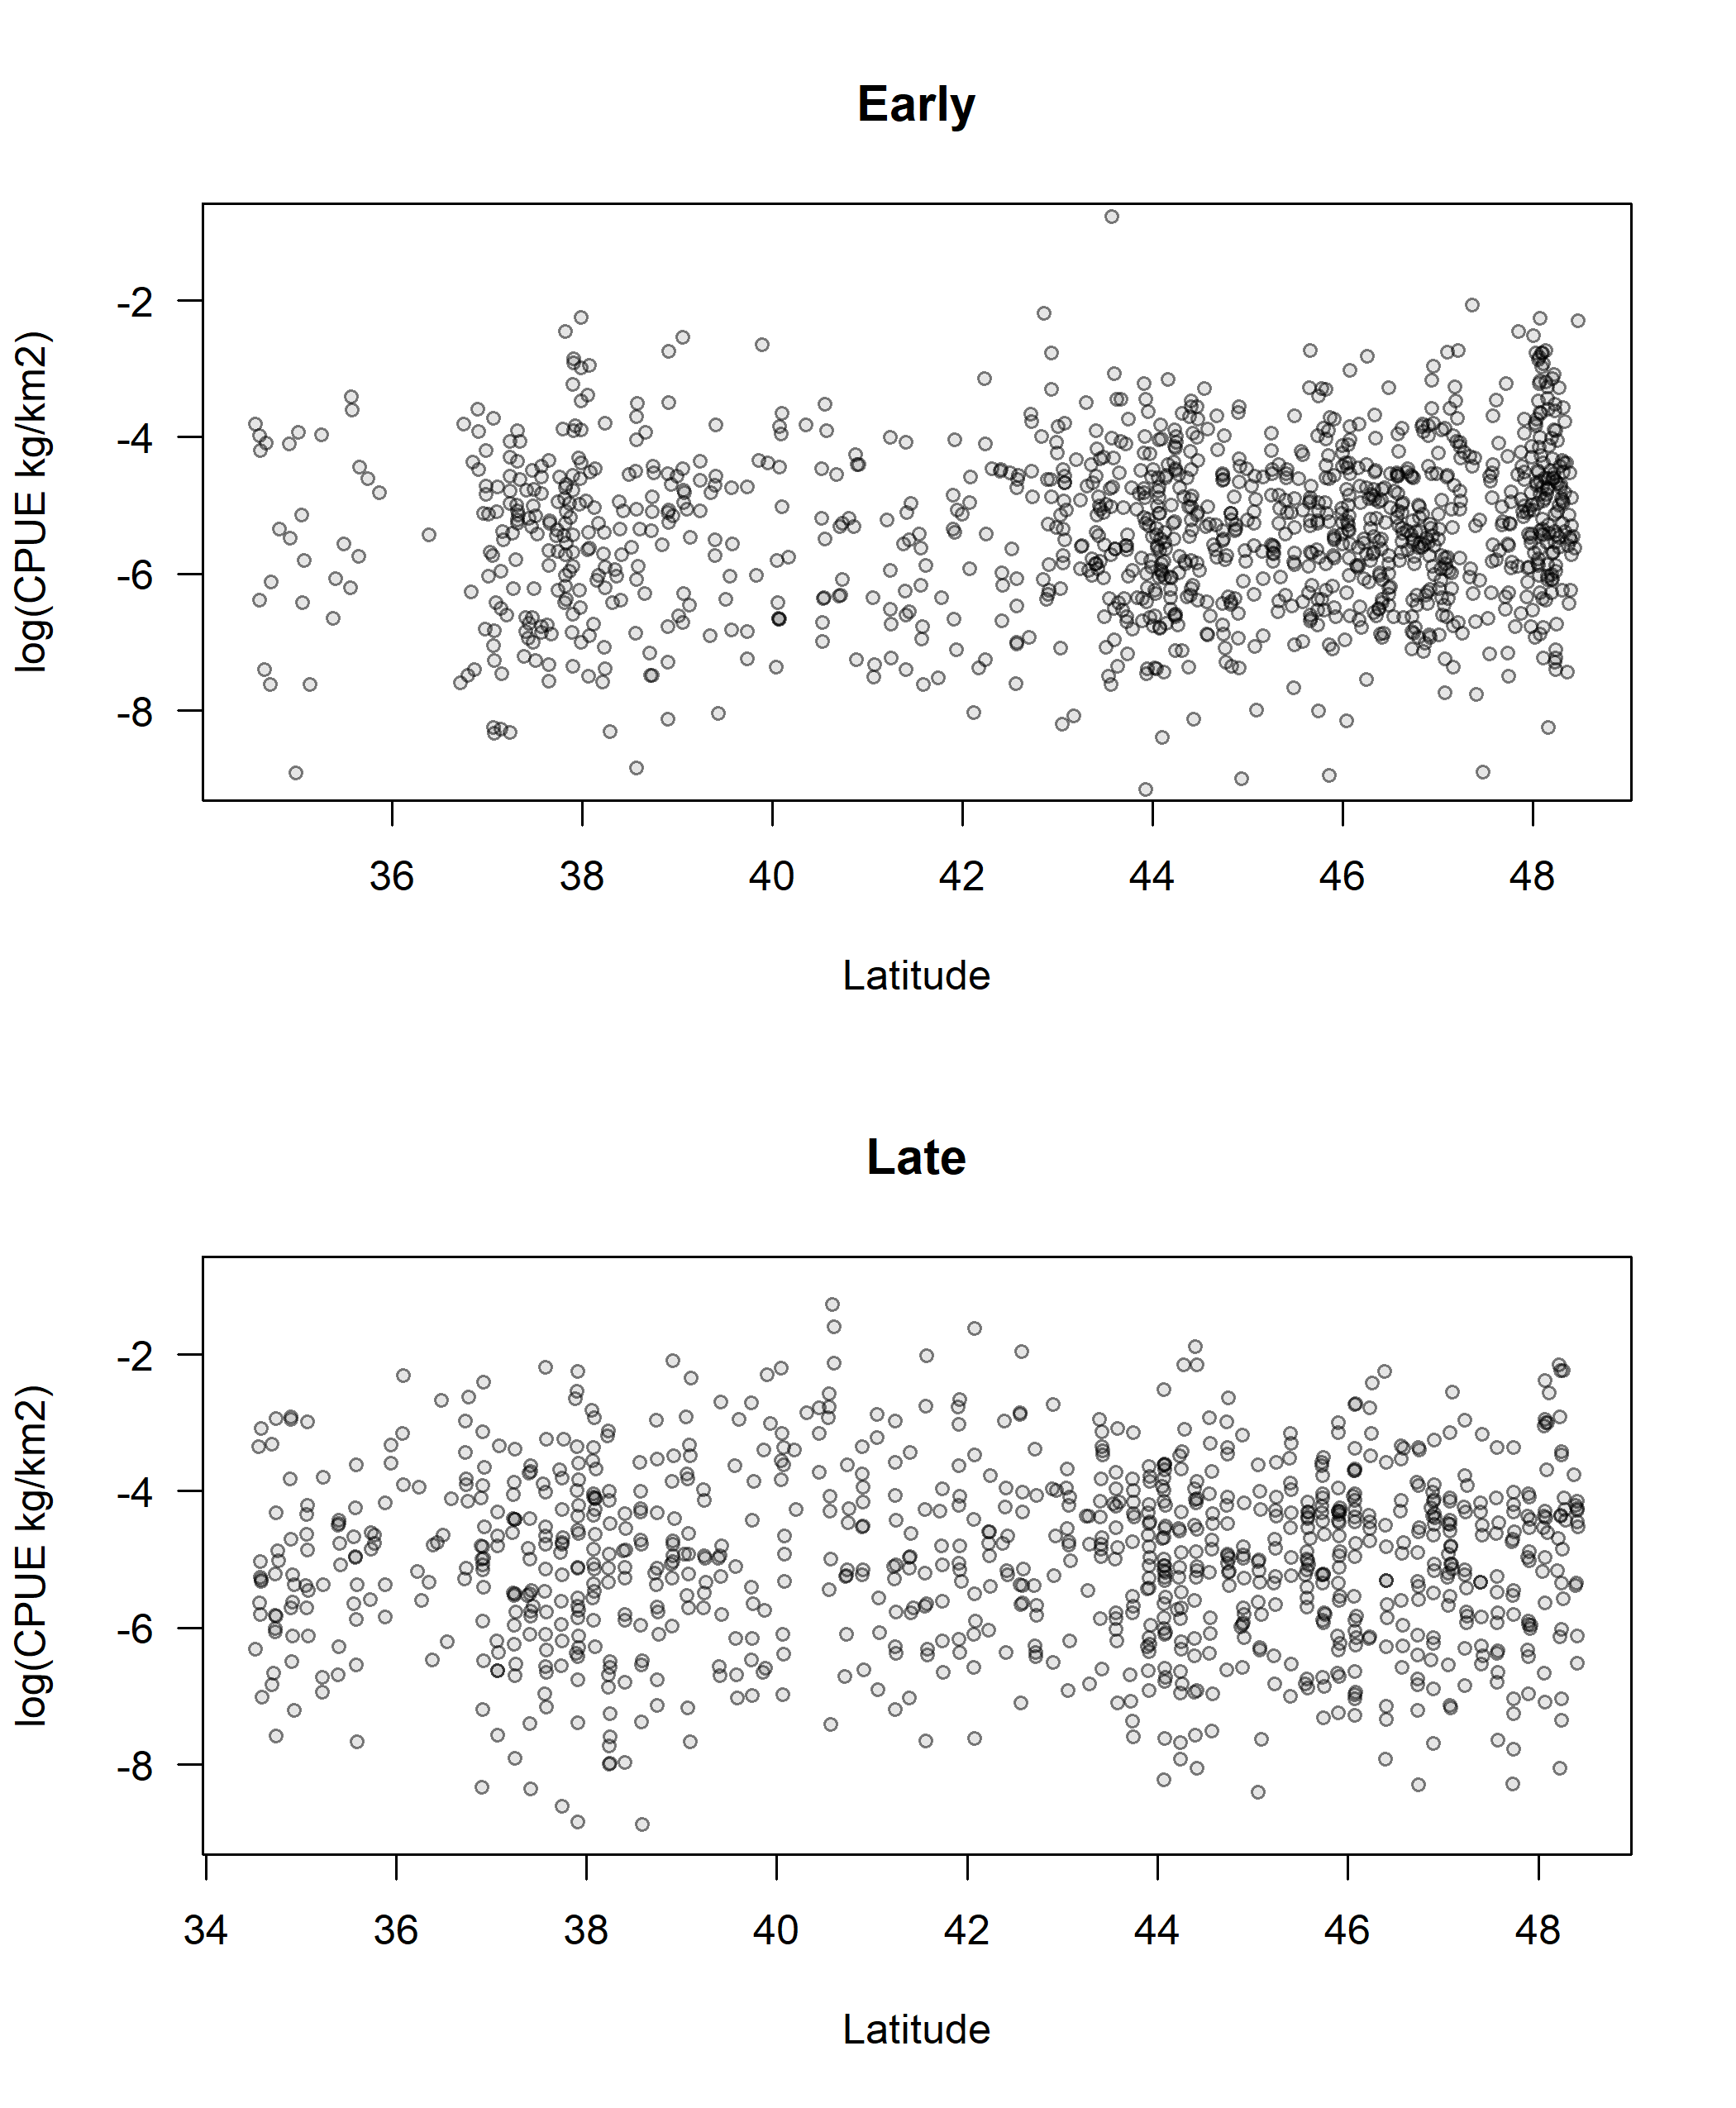
\includegraphics{Figures/Tri_CPUE_Lat.png}
\caption{Catch-per-unit-effort (in log space) by latitude for the
Triennial Survey data. \label{fig:tri_cpue_lat}}
\end{figure}

\FloatBarrier

\begin{figure}
\centering
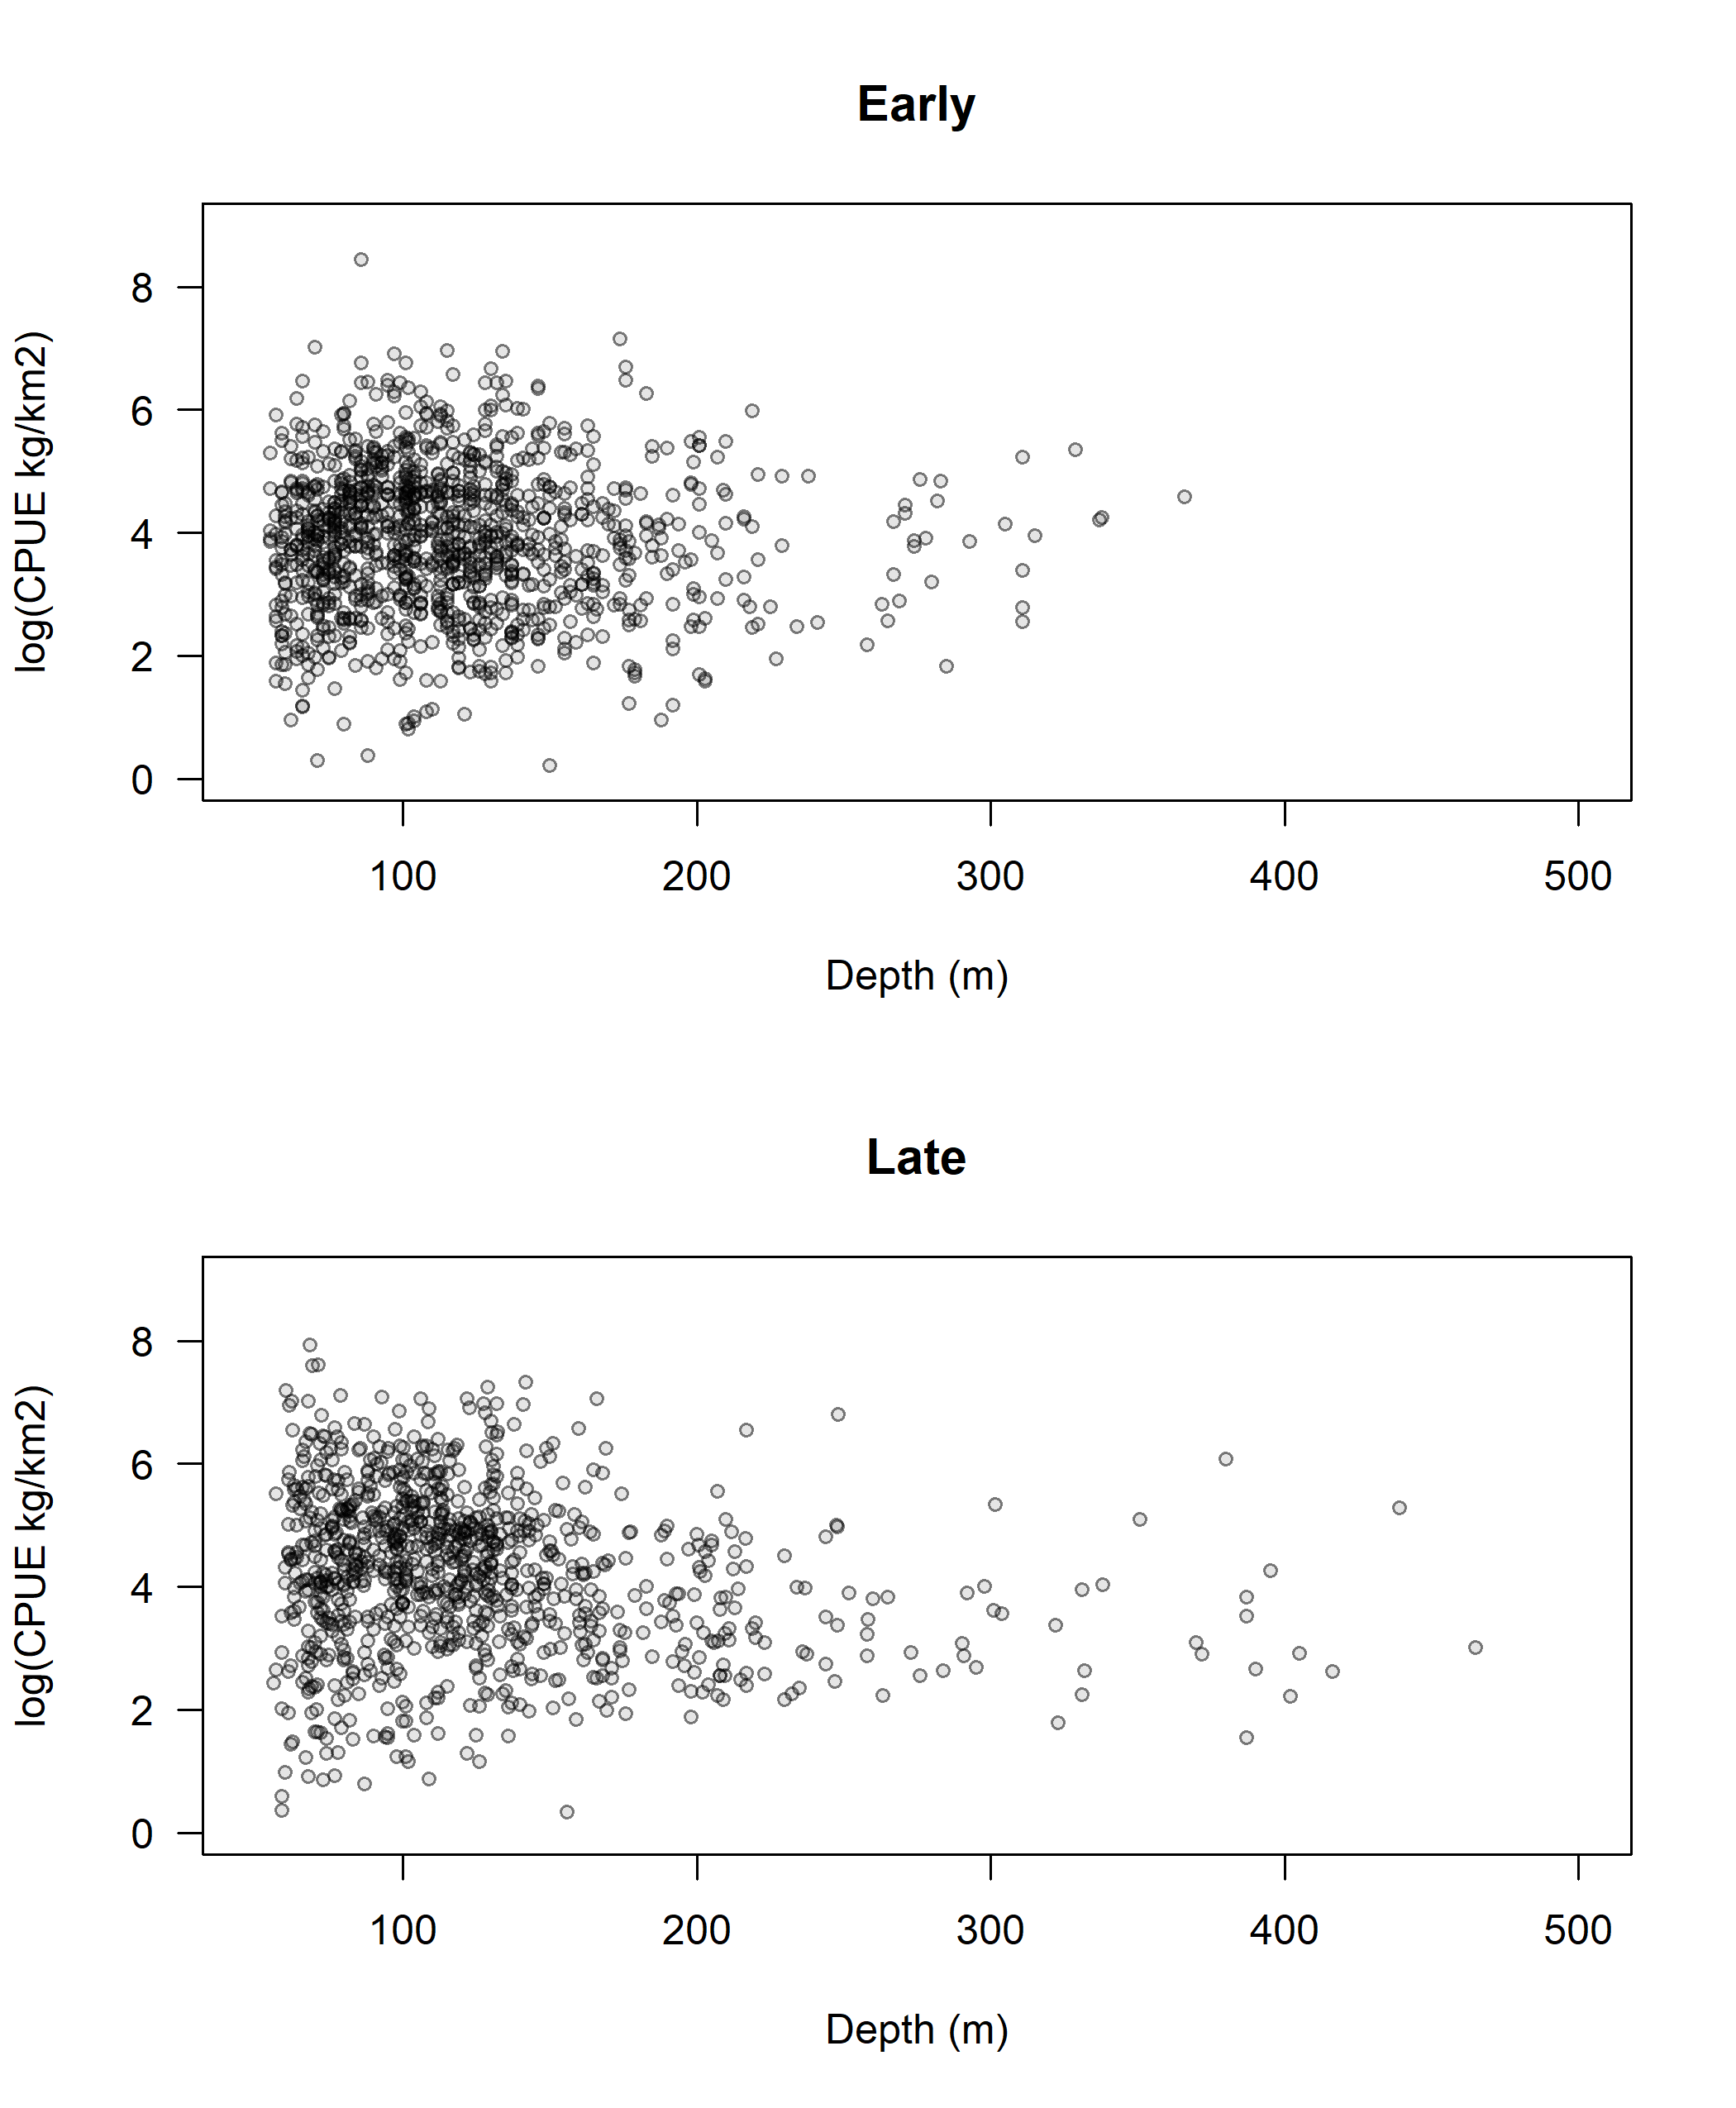
\includegraphics{Figures/Tri_CPUE_Depth.png}
\caption{Catch-per-unit-effort (in log space) by depth (m) for the
Triennial Survey data. \label{fig:tri_cpue_depth}}
\end{figure}

\FloatBarrier

\begin{figure}
\centering
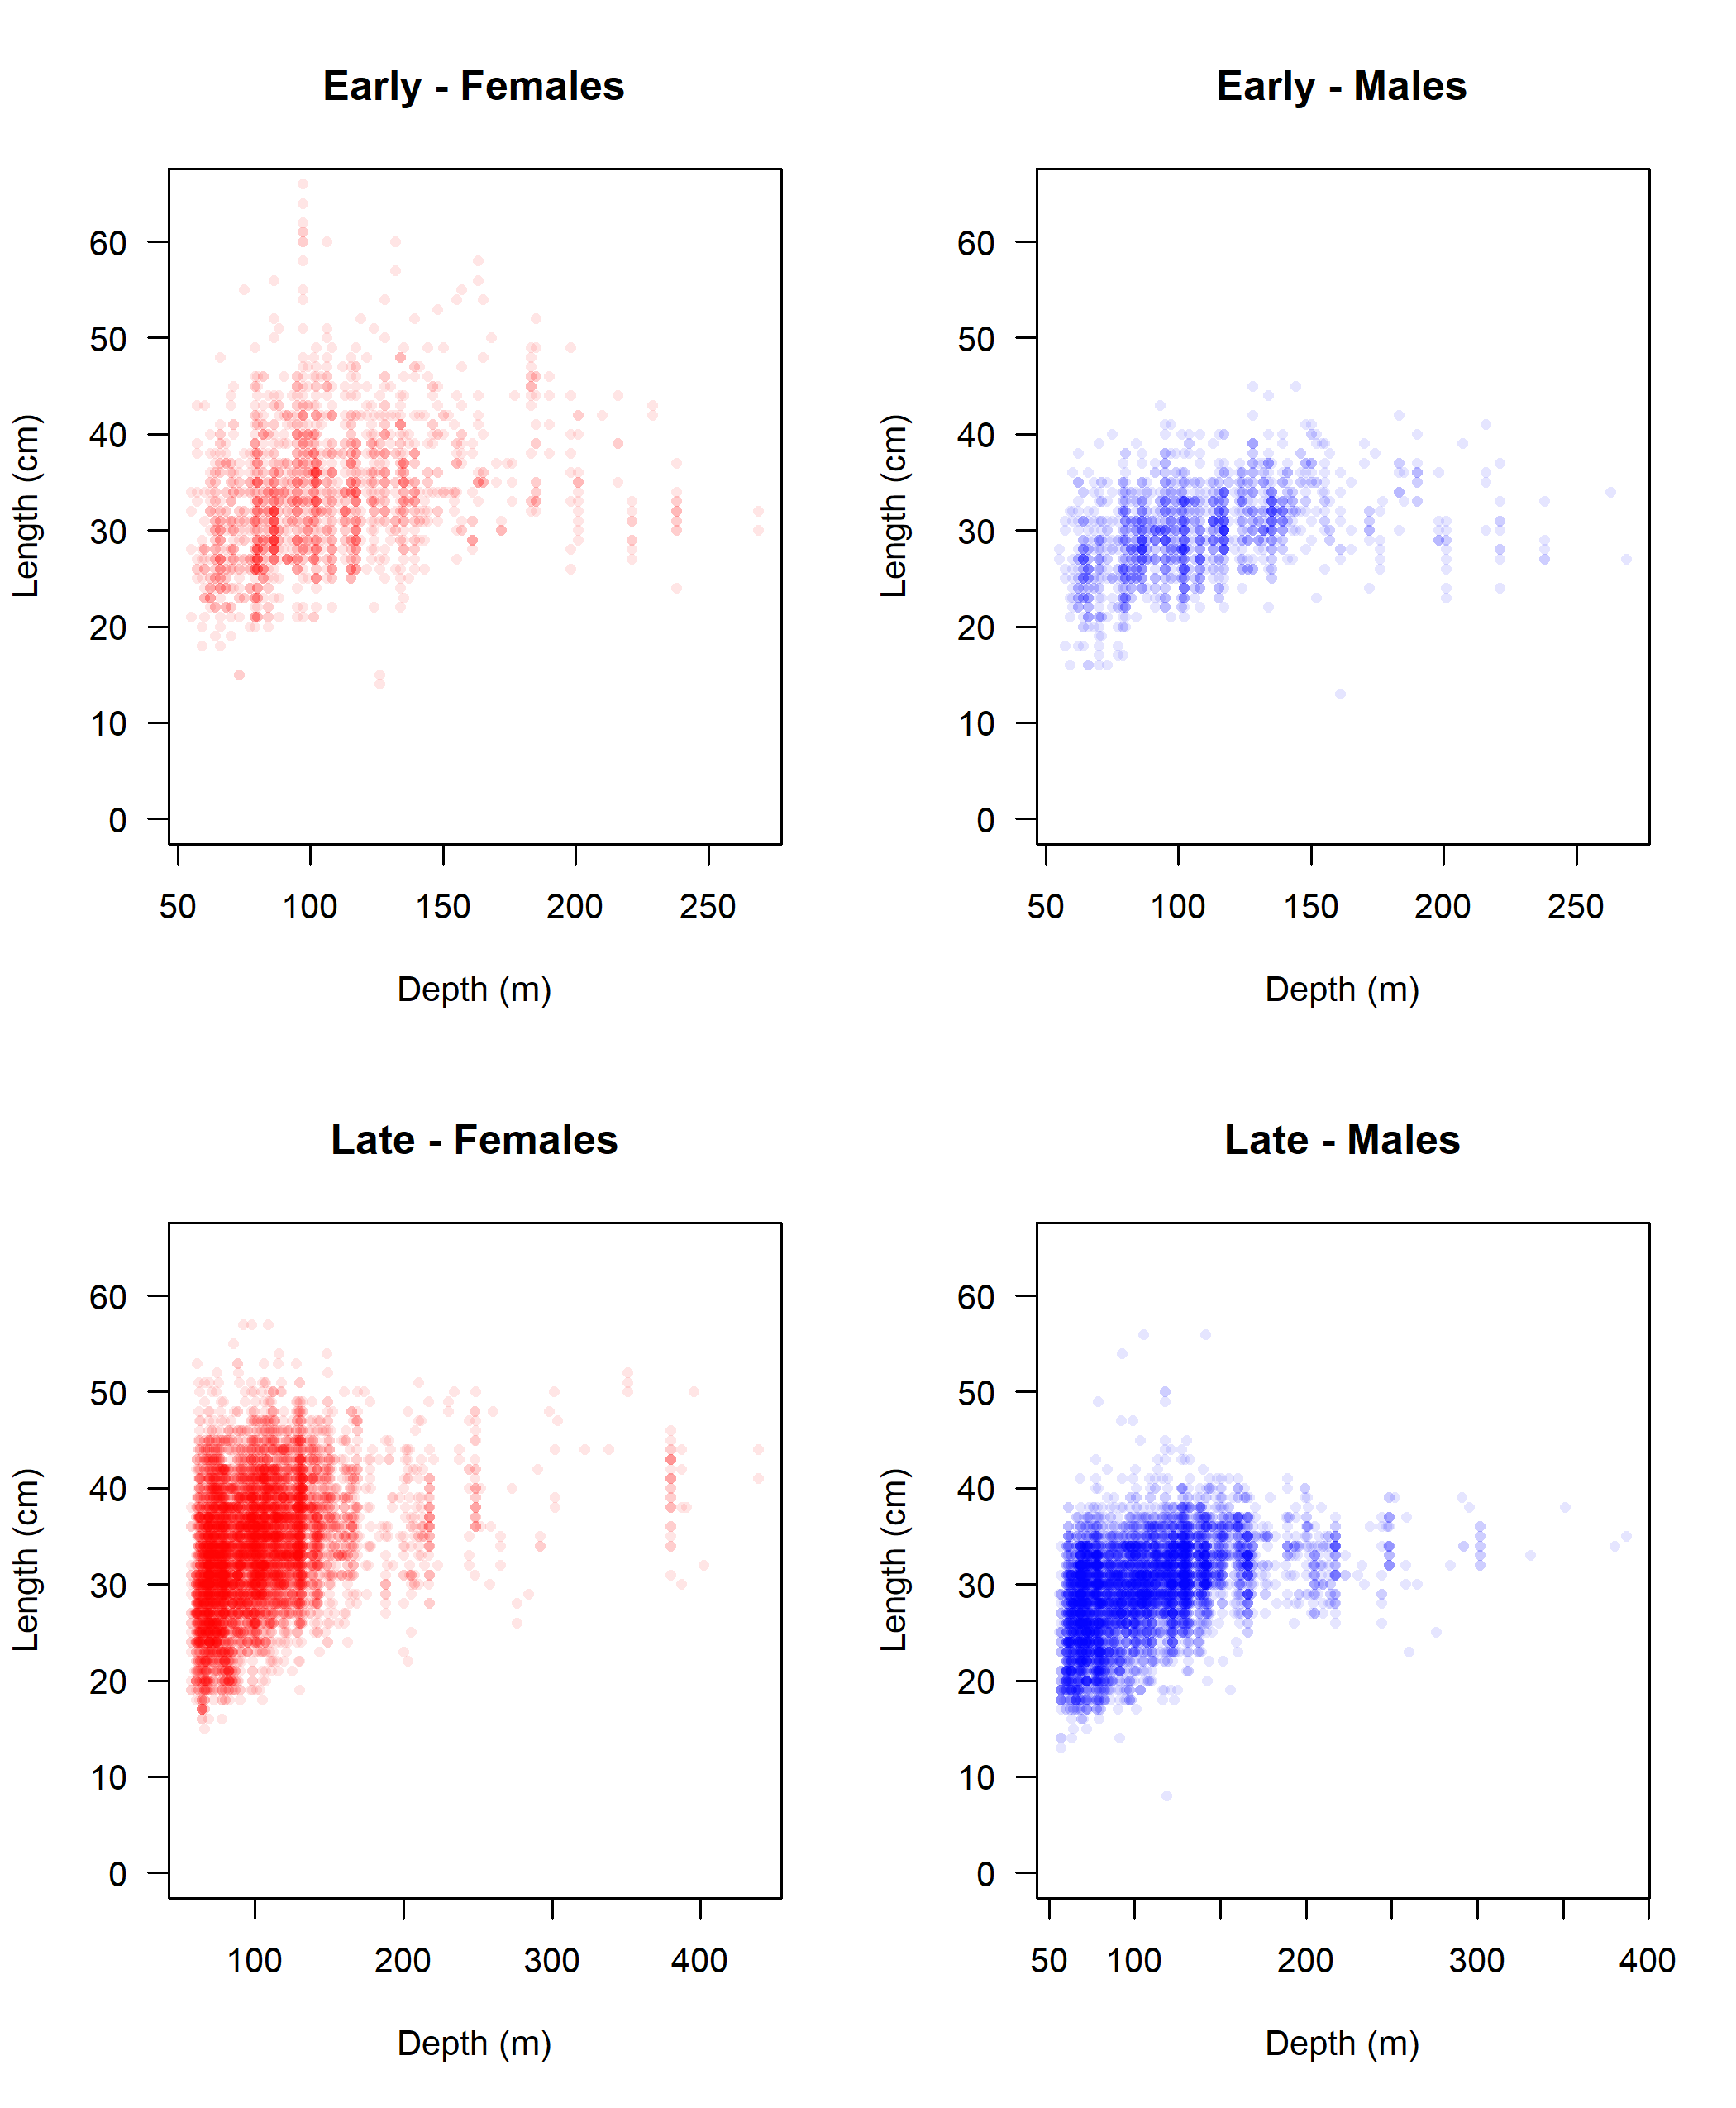
\includegraphics{Figures/Tri_Size_by_Depth.png}
\caption{Length (cm) by depth (m) for the Triennial Survey data.
\label{fig:tri_size_depth}}
\end{figure}

\FloatBarrier

\begin{figure}
\centering
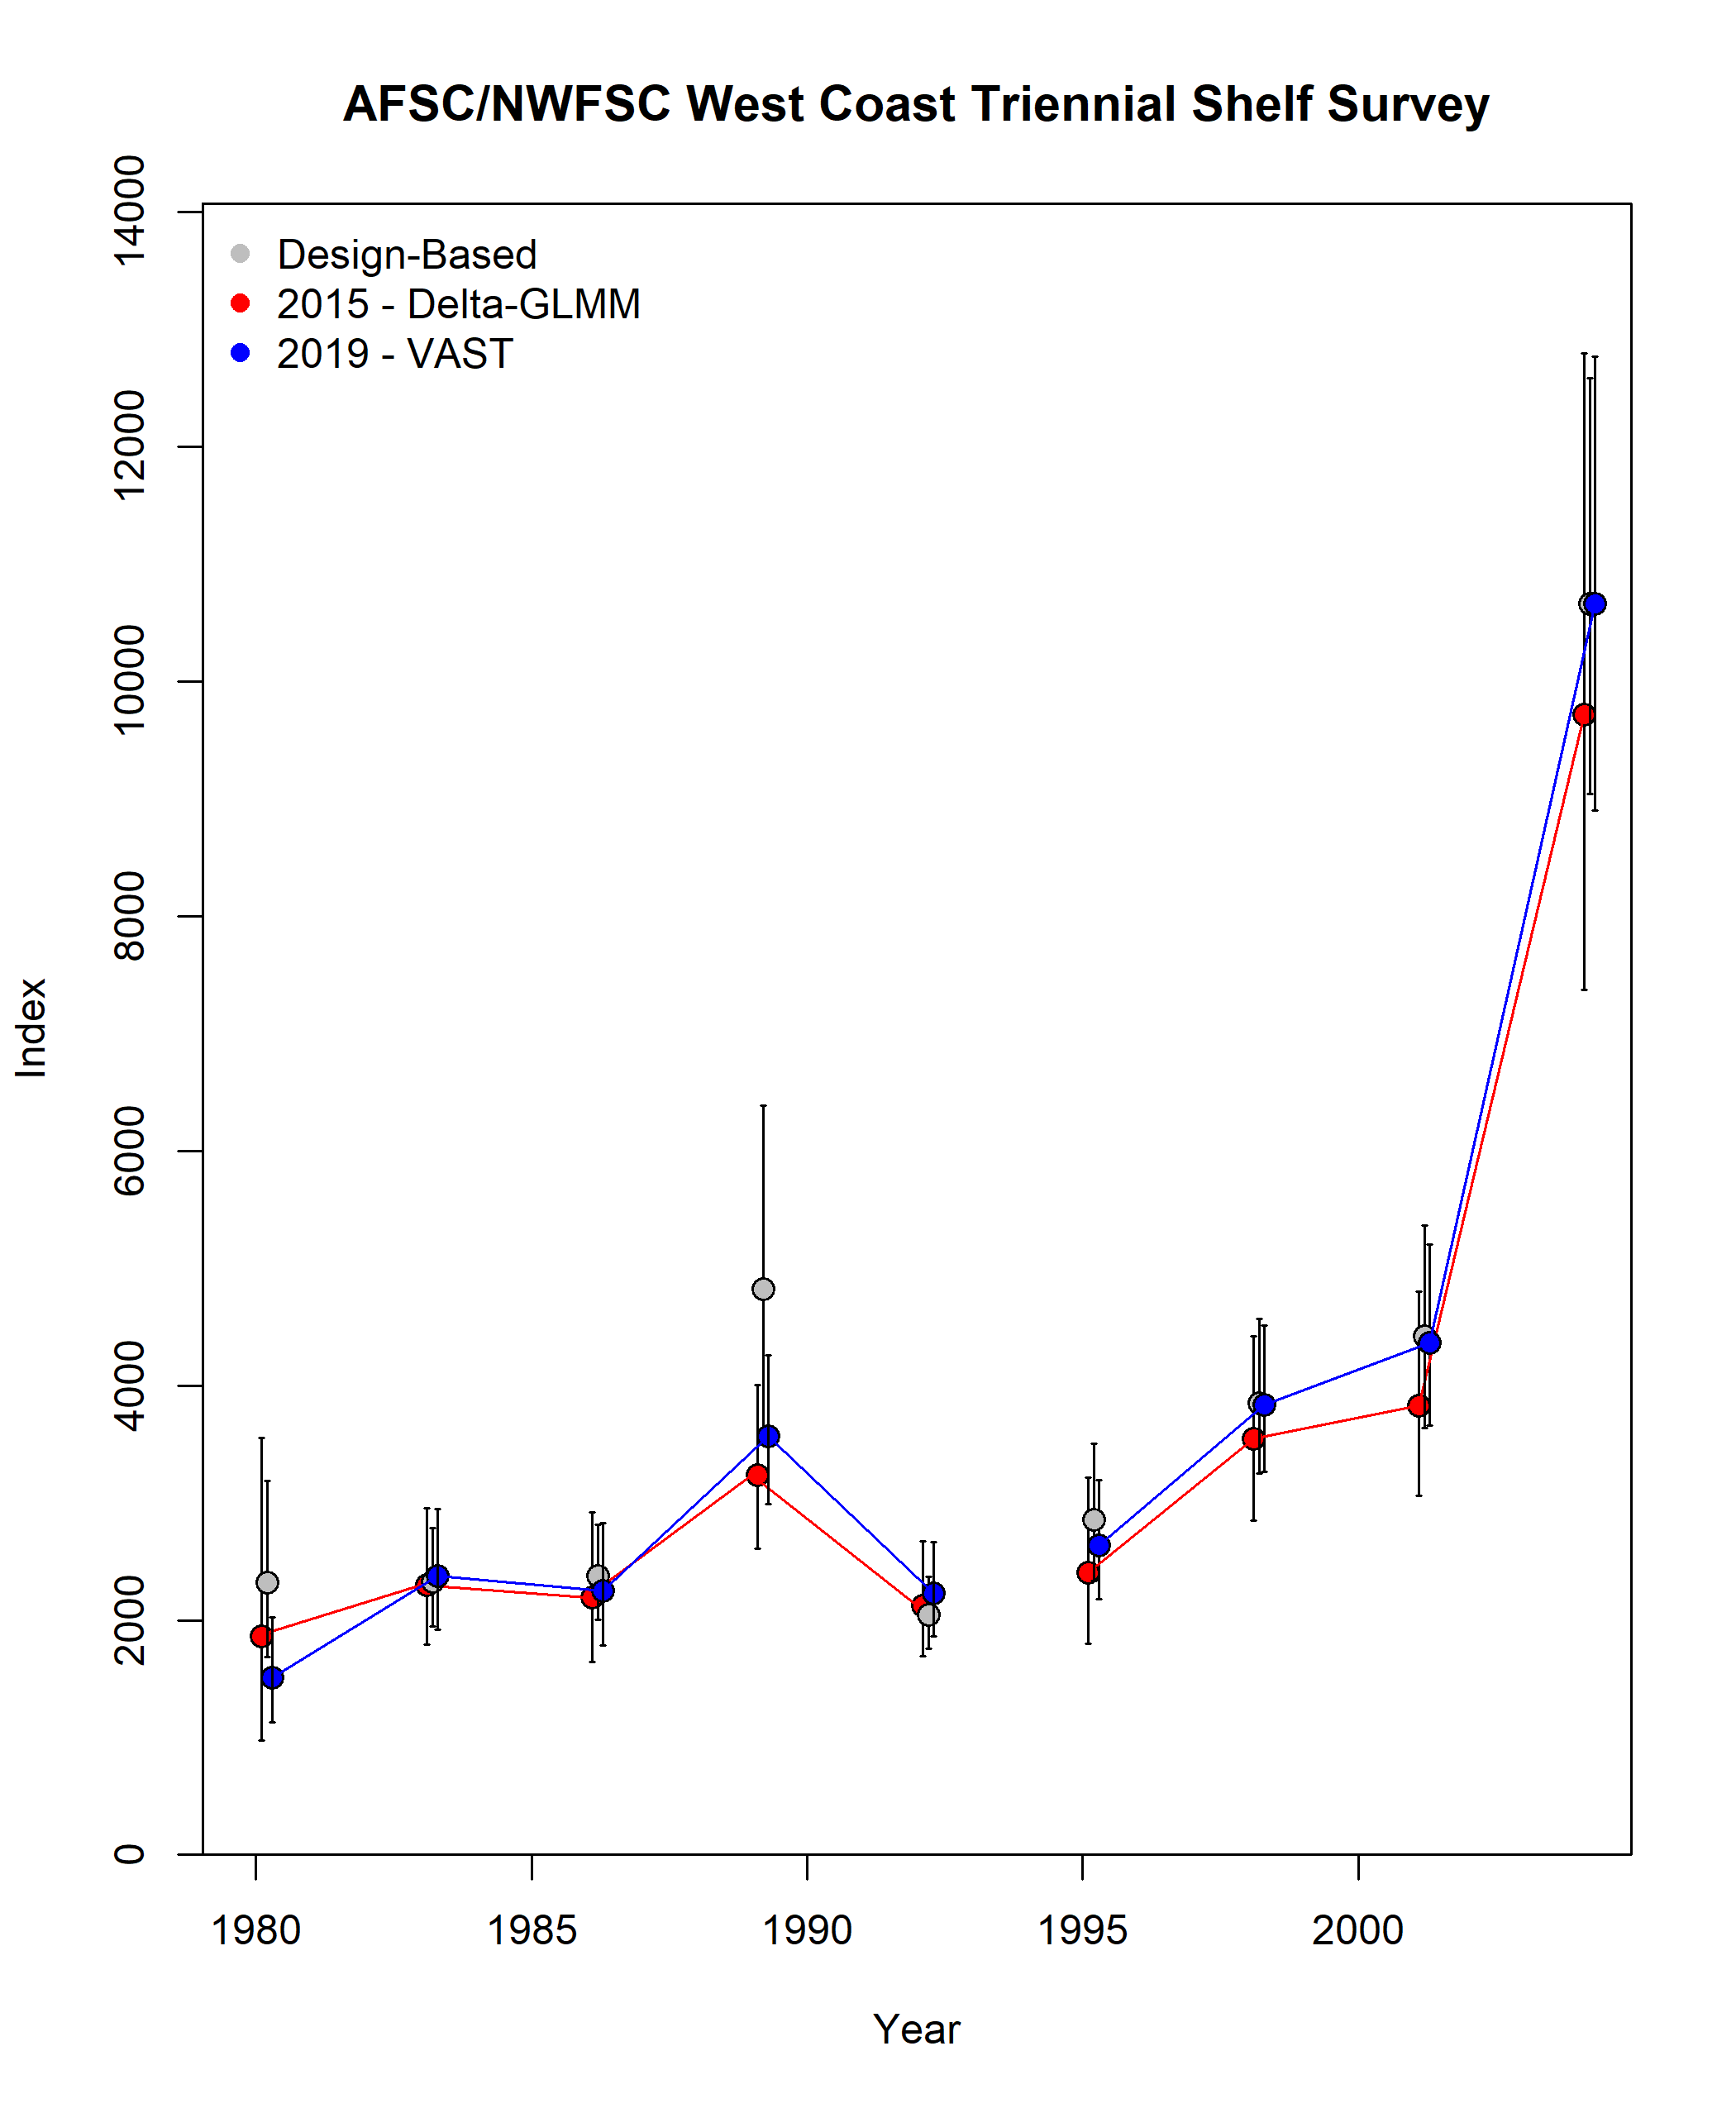
\includegraphics{Figures/Triennial_Index_w_VAST.png}
\caption{Estimated index of abundance from the Triennial Survey data
compared to the design-based index and the index from the 2015 update
assessment. \label{fig:tri_index}}
\end{figure}

\FloatBarrier

\begin{figure}
\centering
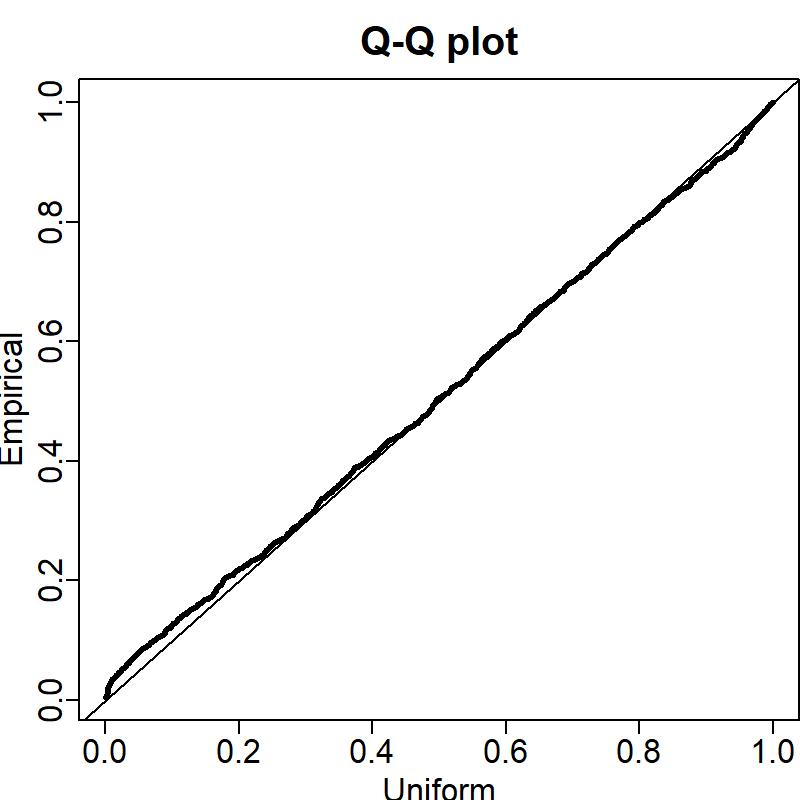
\includegraphics{Figures/tri_early_Posterior_Predictive-Histogram-1.jpg}
\caption{QQ plot for the Triennial Early Survey data.
\label{fig:tri_early_qq}}
\end{figure}

\FloatBarrier

\begin{figure}
\centering
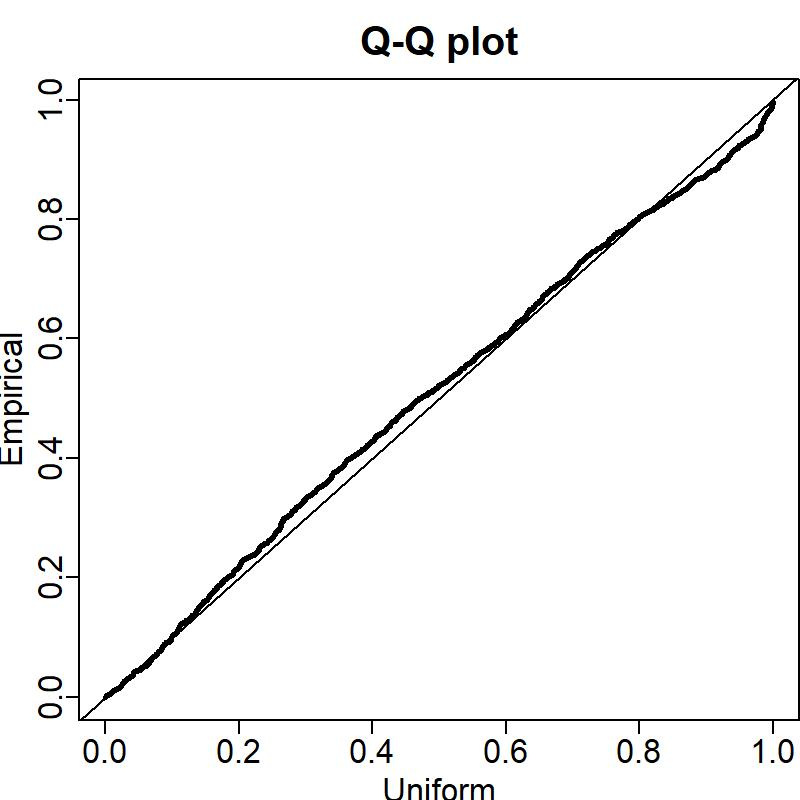
\includegraphics{Figures/tri_late_Posterior_Predictive-Histogram-1.jpg}
\caption{QQ plot for the Triennial Late Survey data.
\label{fig:tri_late_qq}}
\end{figure}

\FloatBarrier

\begin{figure}
\centering
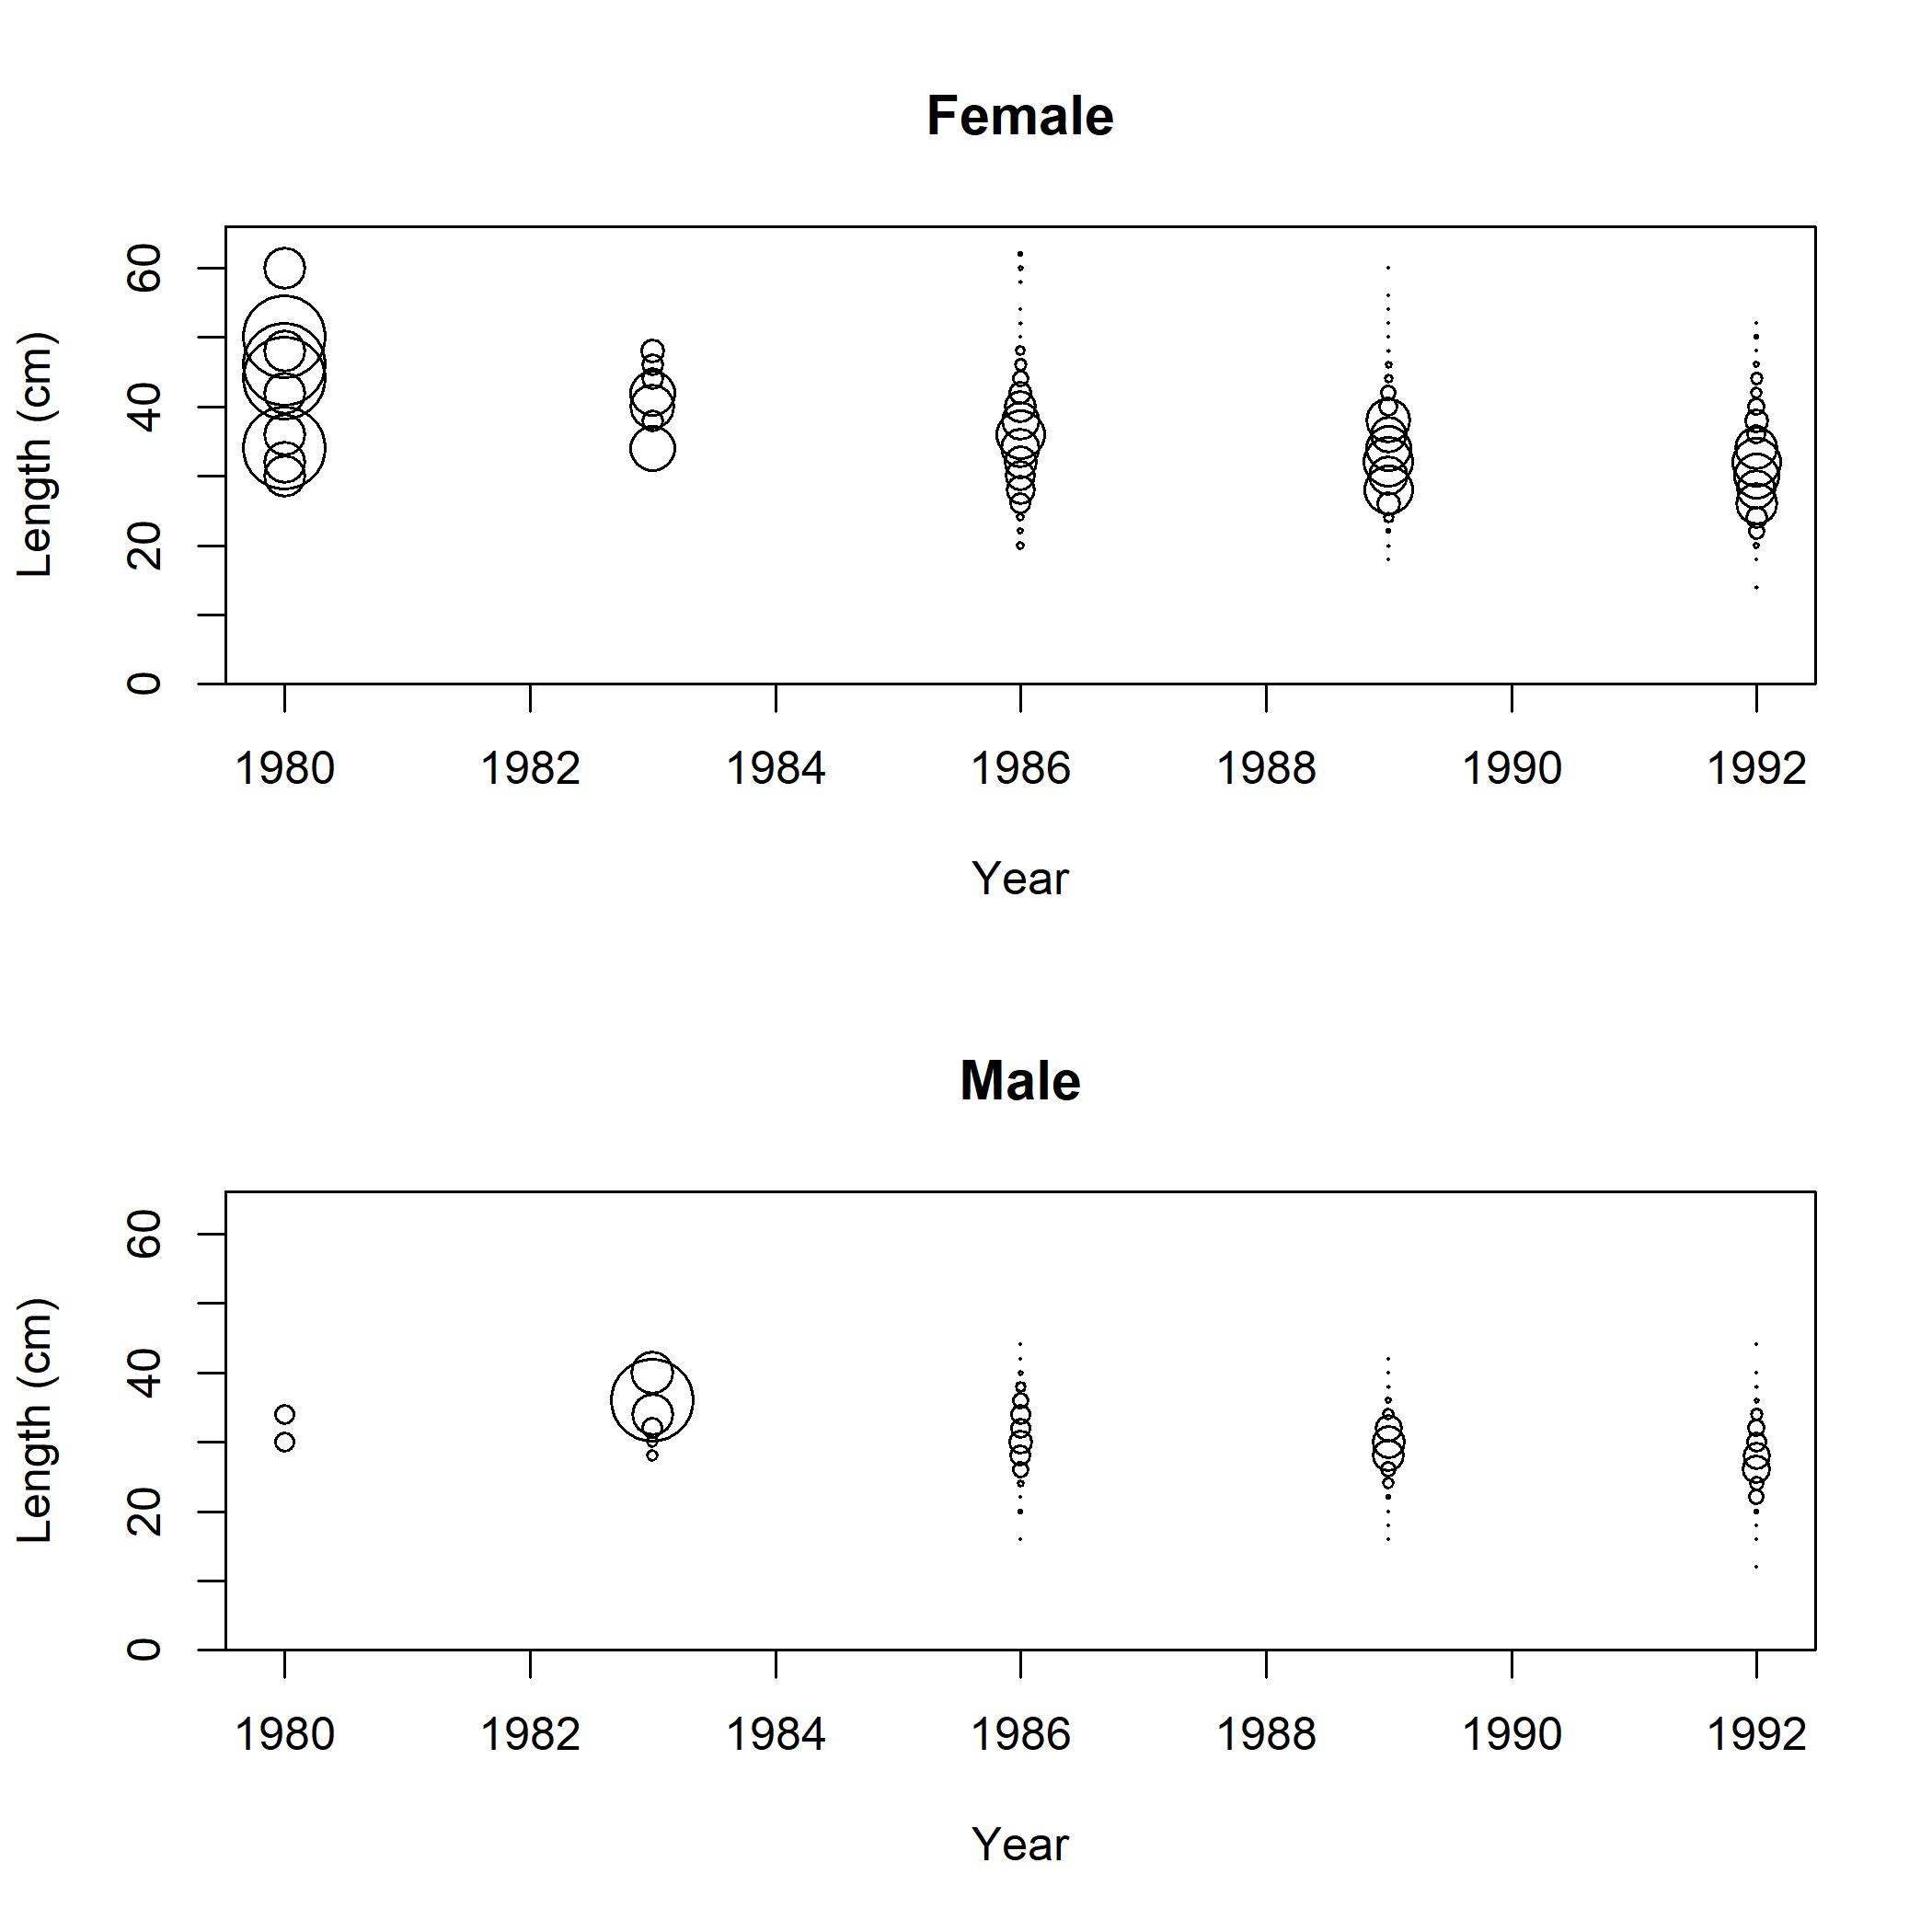
\includegraphics{Figures/Triennial Early_Length_Frequency.png}
\caption{Length frequency by sex for the Triennial Early Survey data.
\label{fig:tri_early_len_freq}}
\end{figure}

\FloatBarrier

\begin{figure}
\centering
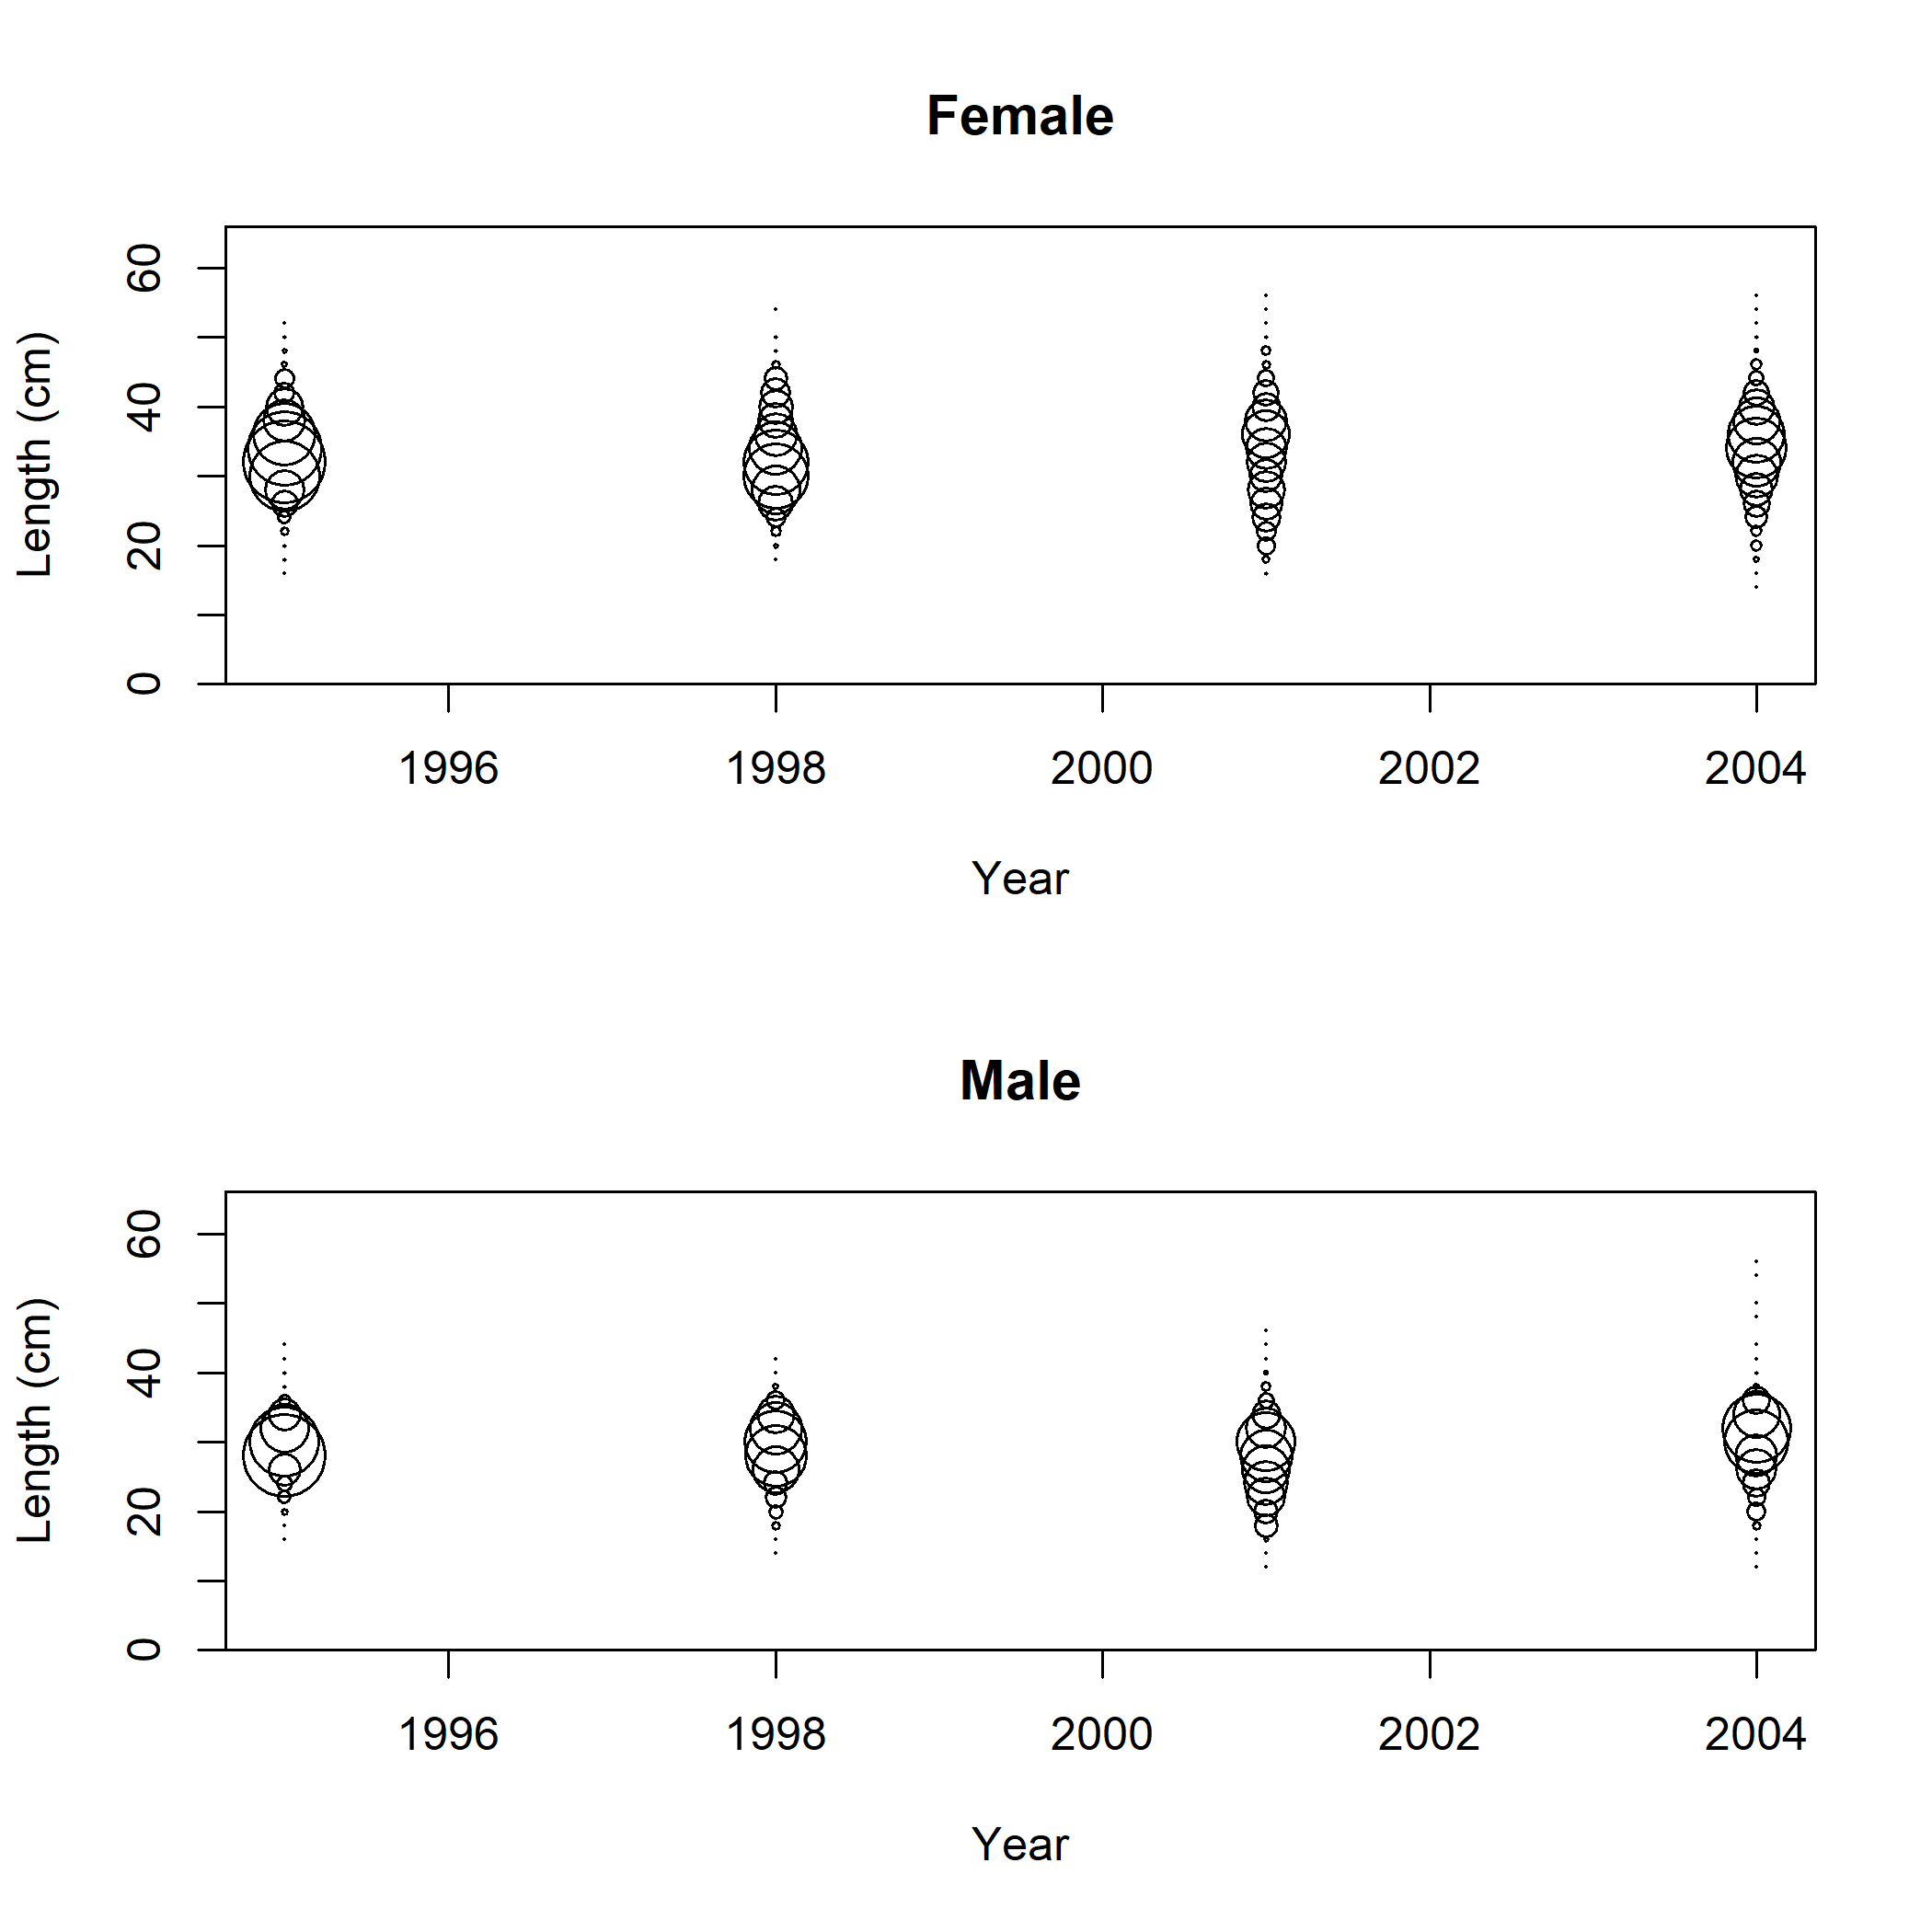
\includegraphics{Figures/Triennial Late_Length_Frequency.png}
\caption{Length frequency by sex for the Triennial Late Survey data.
\label{fig:tri_late_len_freq}}
\end{figure}

\FloatBarrier

\begin{figure}
\centering
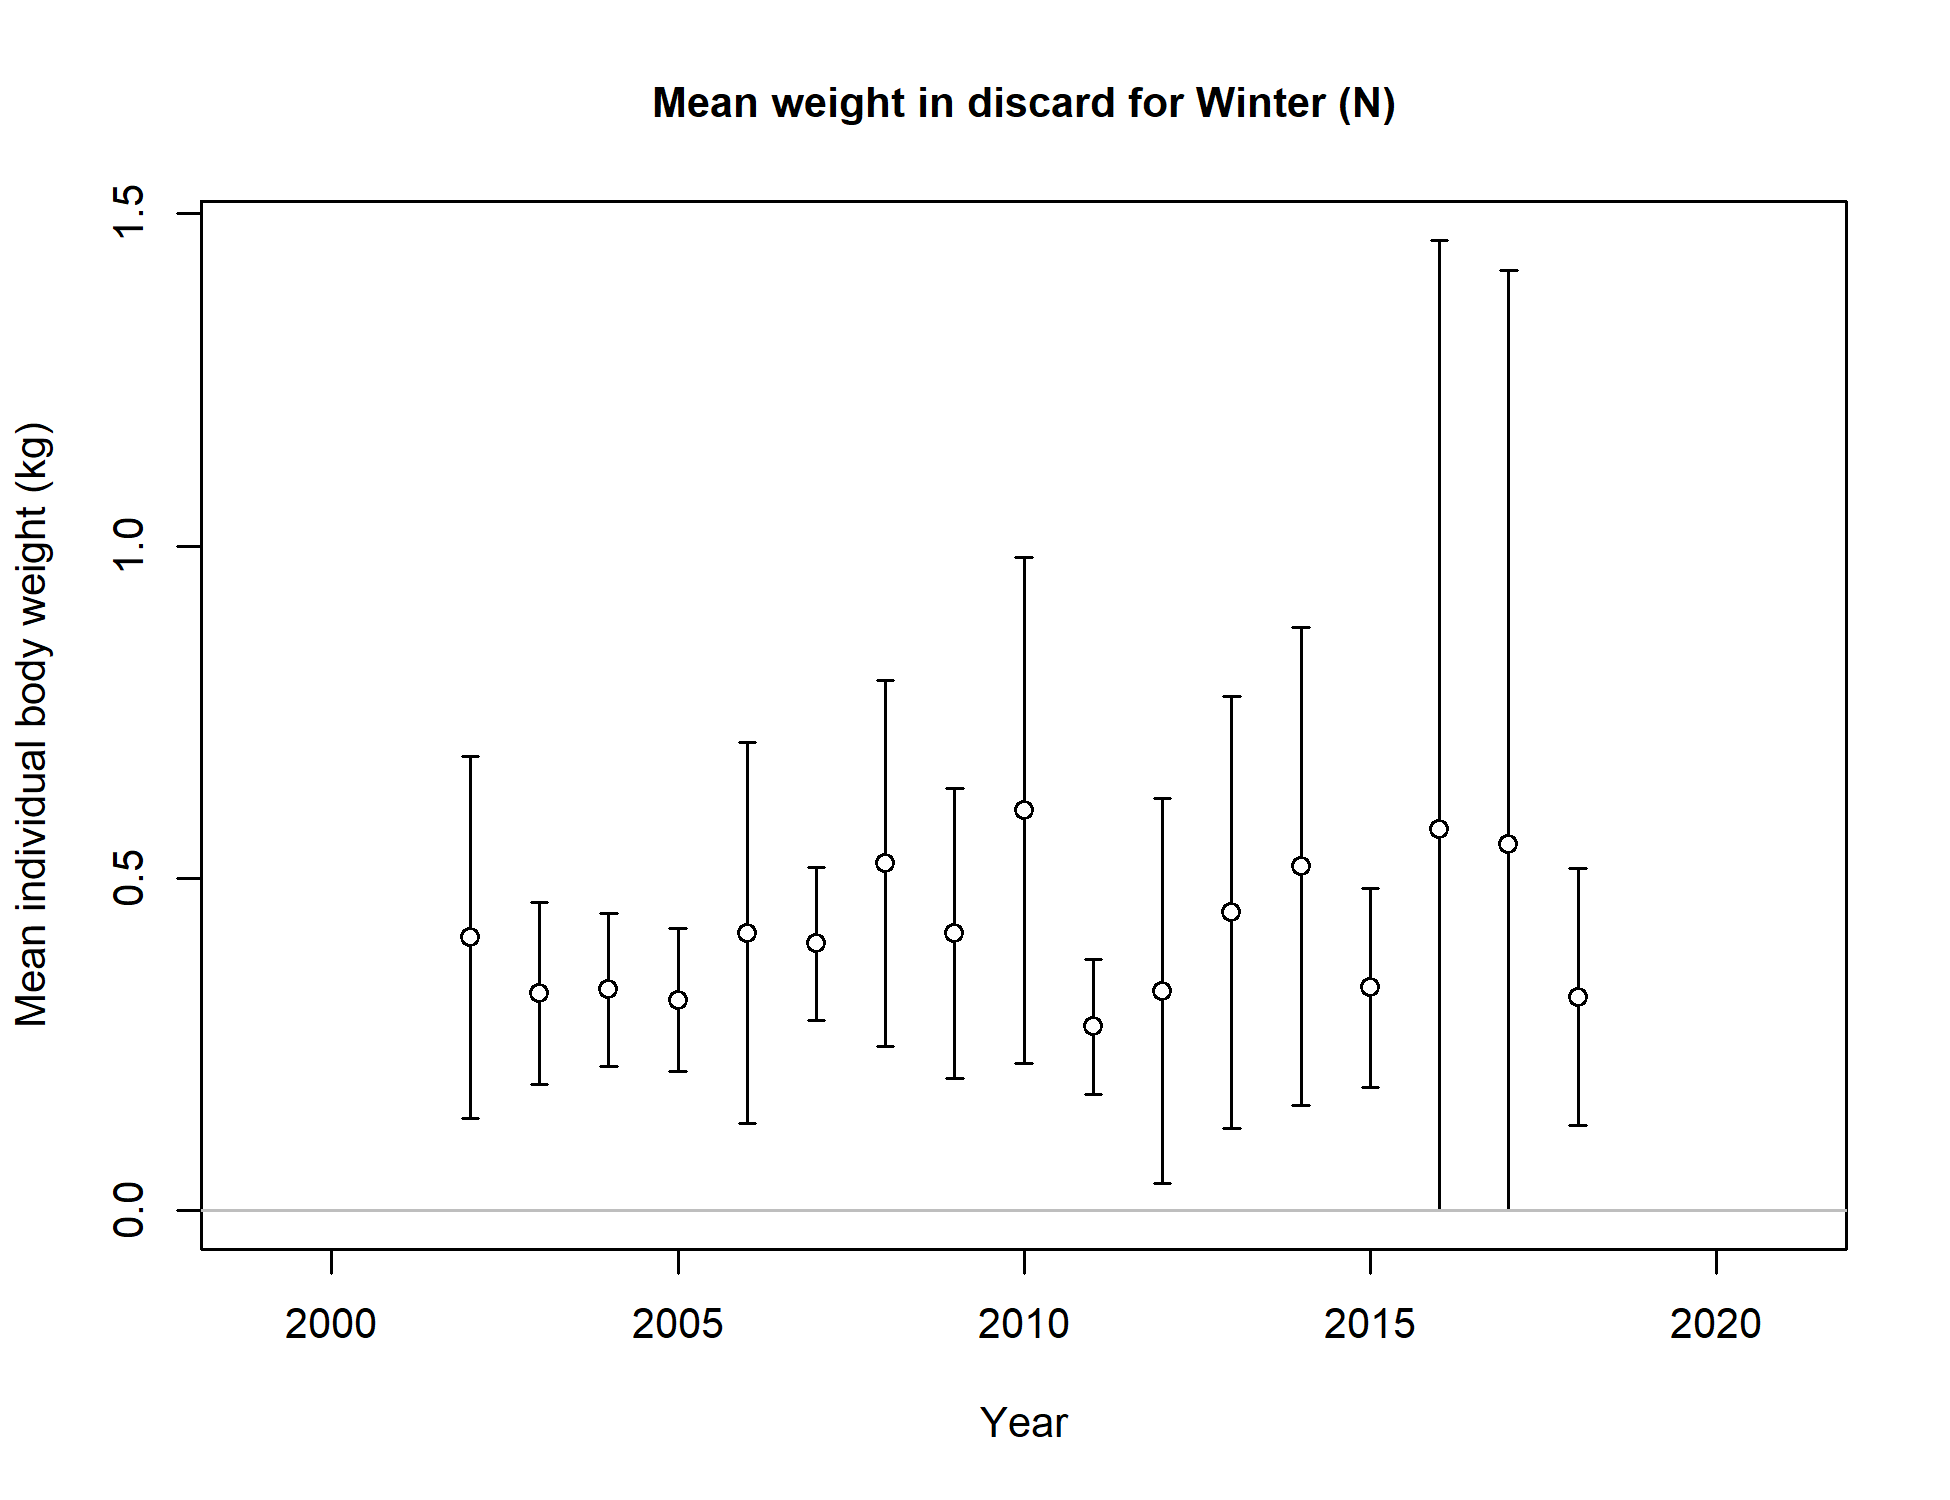
\includegraphics{r4ss/plots_mod1/bodywt_data_fltWinter (N).png}
\caption{Northern winter fishery mean body weights of discarded fish for
petrale sole. \label{fig:nw_bodywt}}
\end{figure}

\FloatBarrier

\begin{figure}
\centering
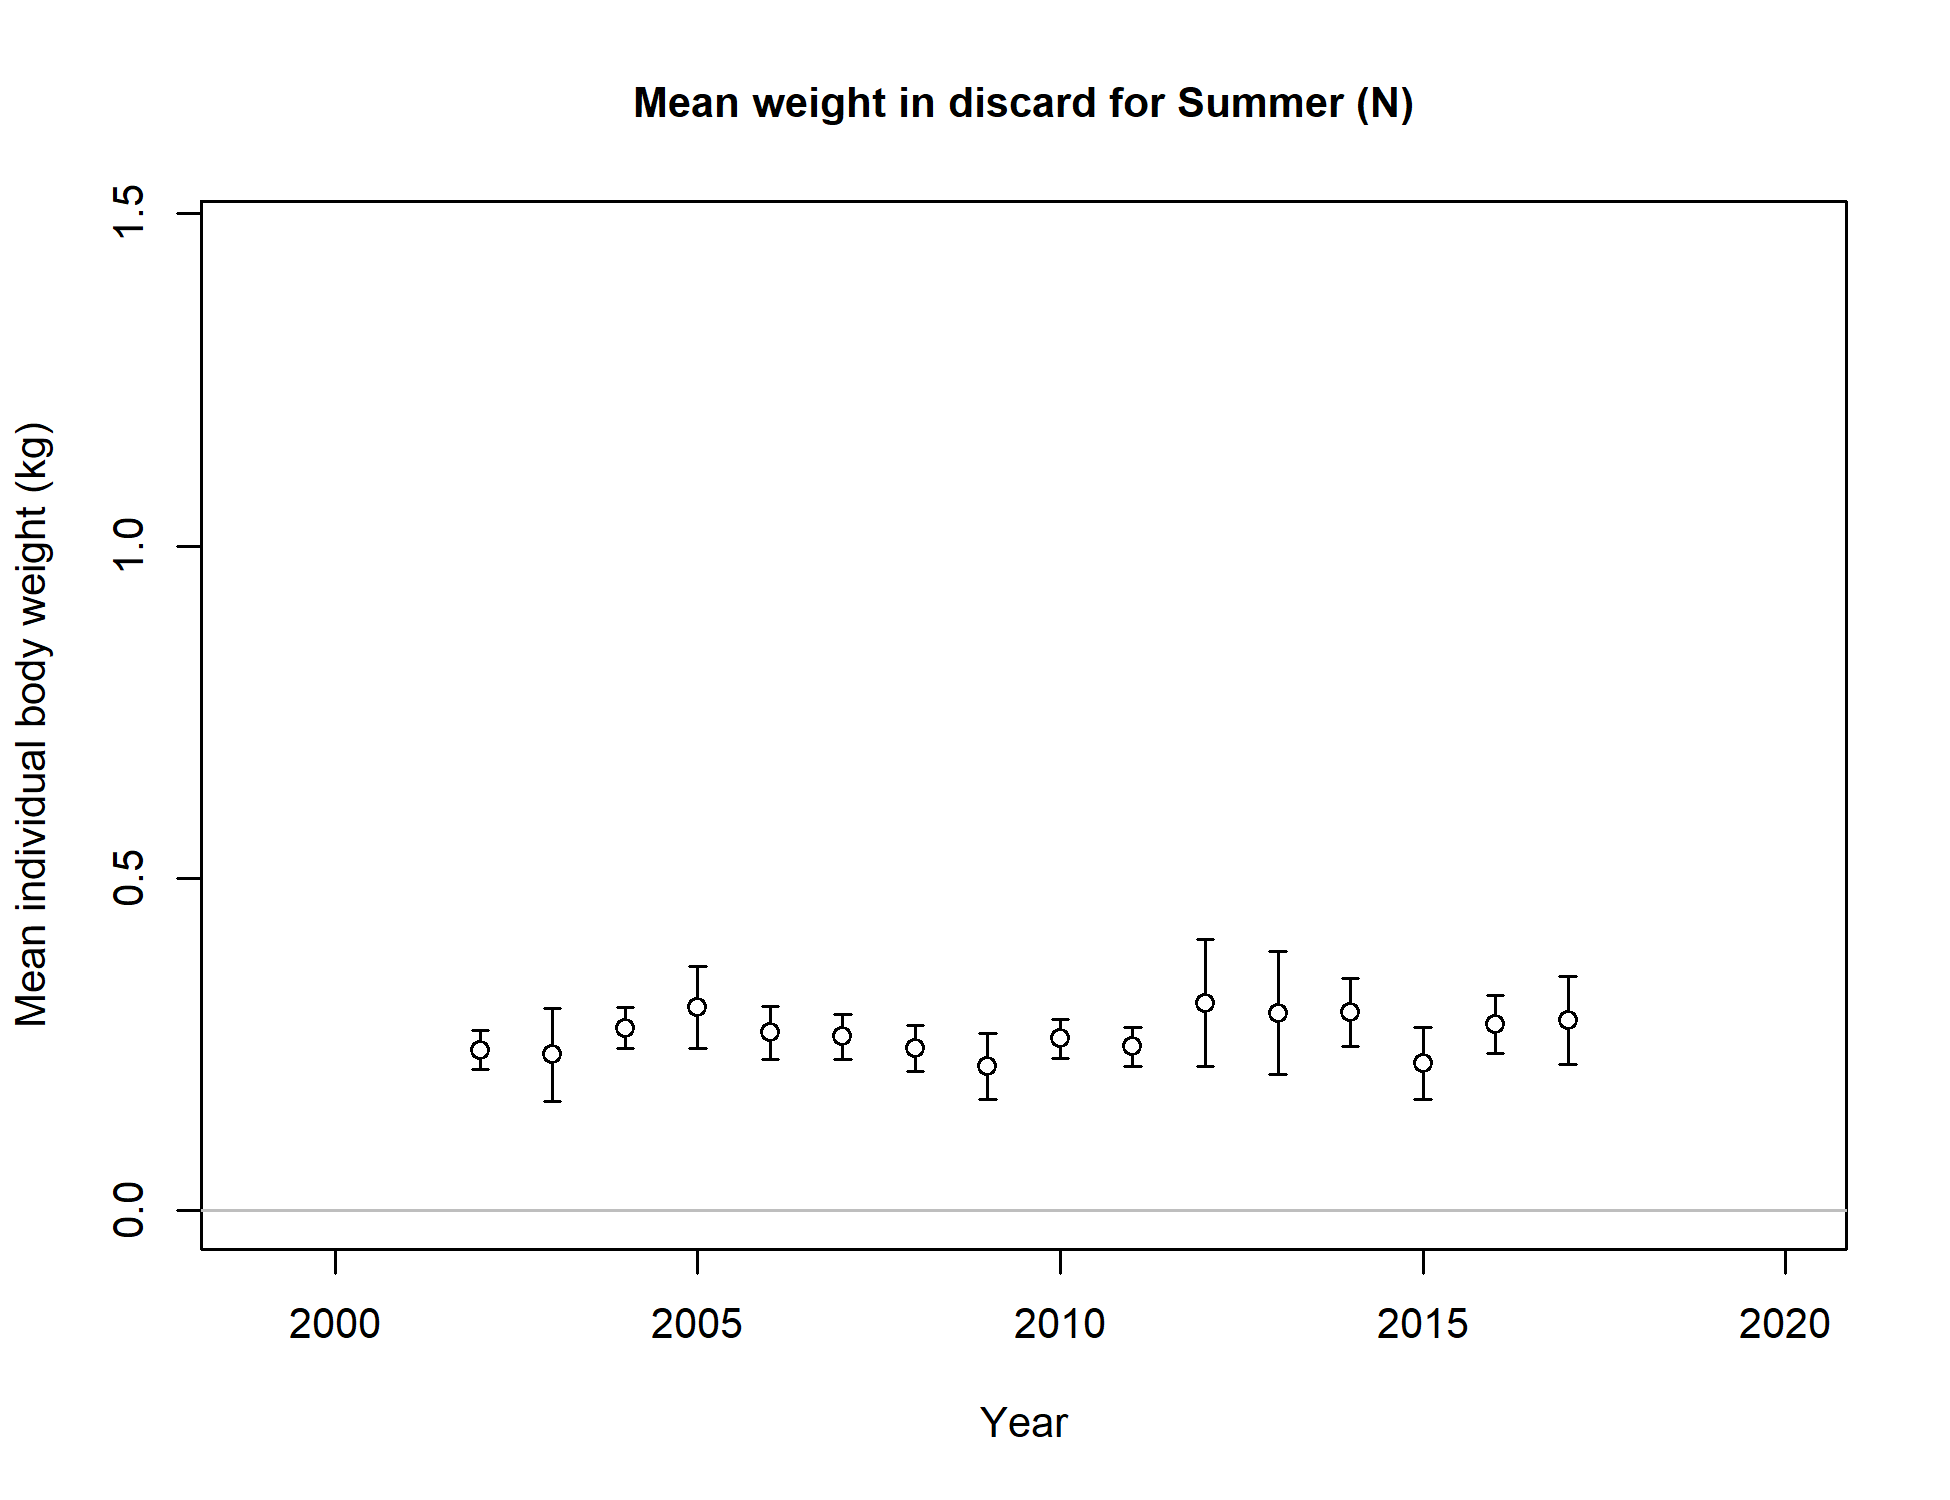
\includegraphics{r4ss/plots_mod1/bodywt_data_fltSummer (N).png}
\caption{Northern summer fishery mean body weights of discarded fish for
petrale sole. \label{fig:ns_bodywt}}
\end{figure}

\FloatBarrier

\begin{figure}
\centering
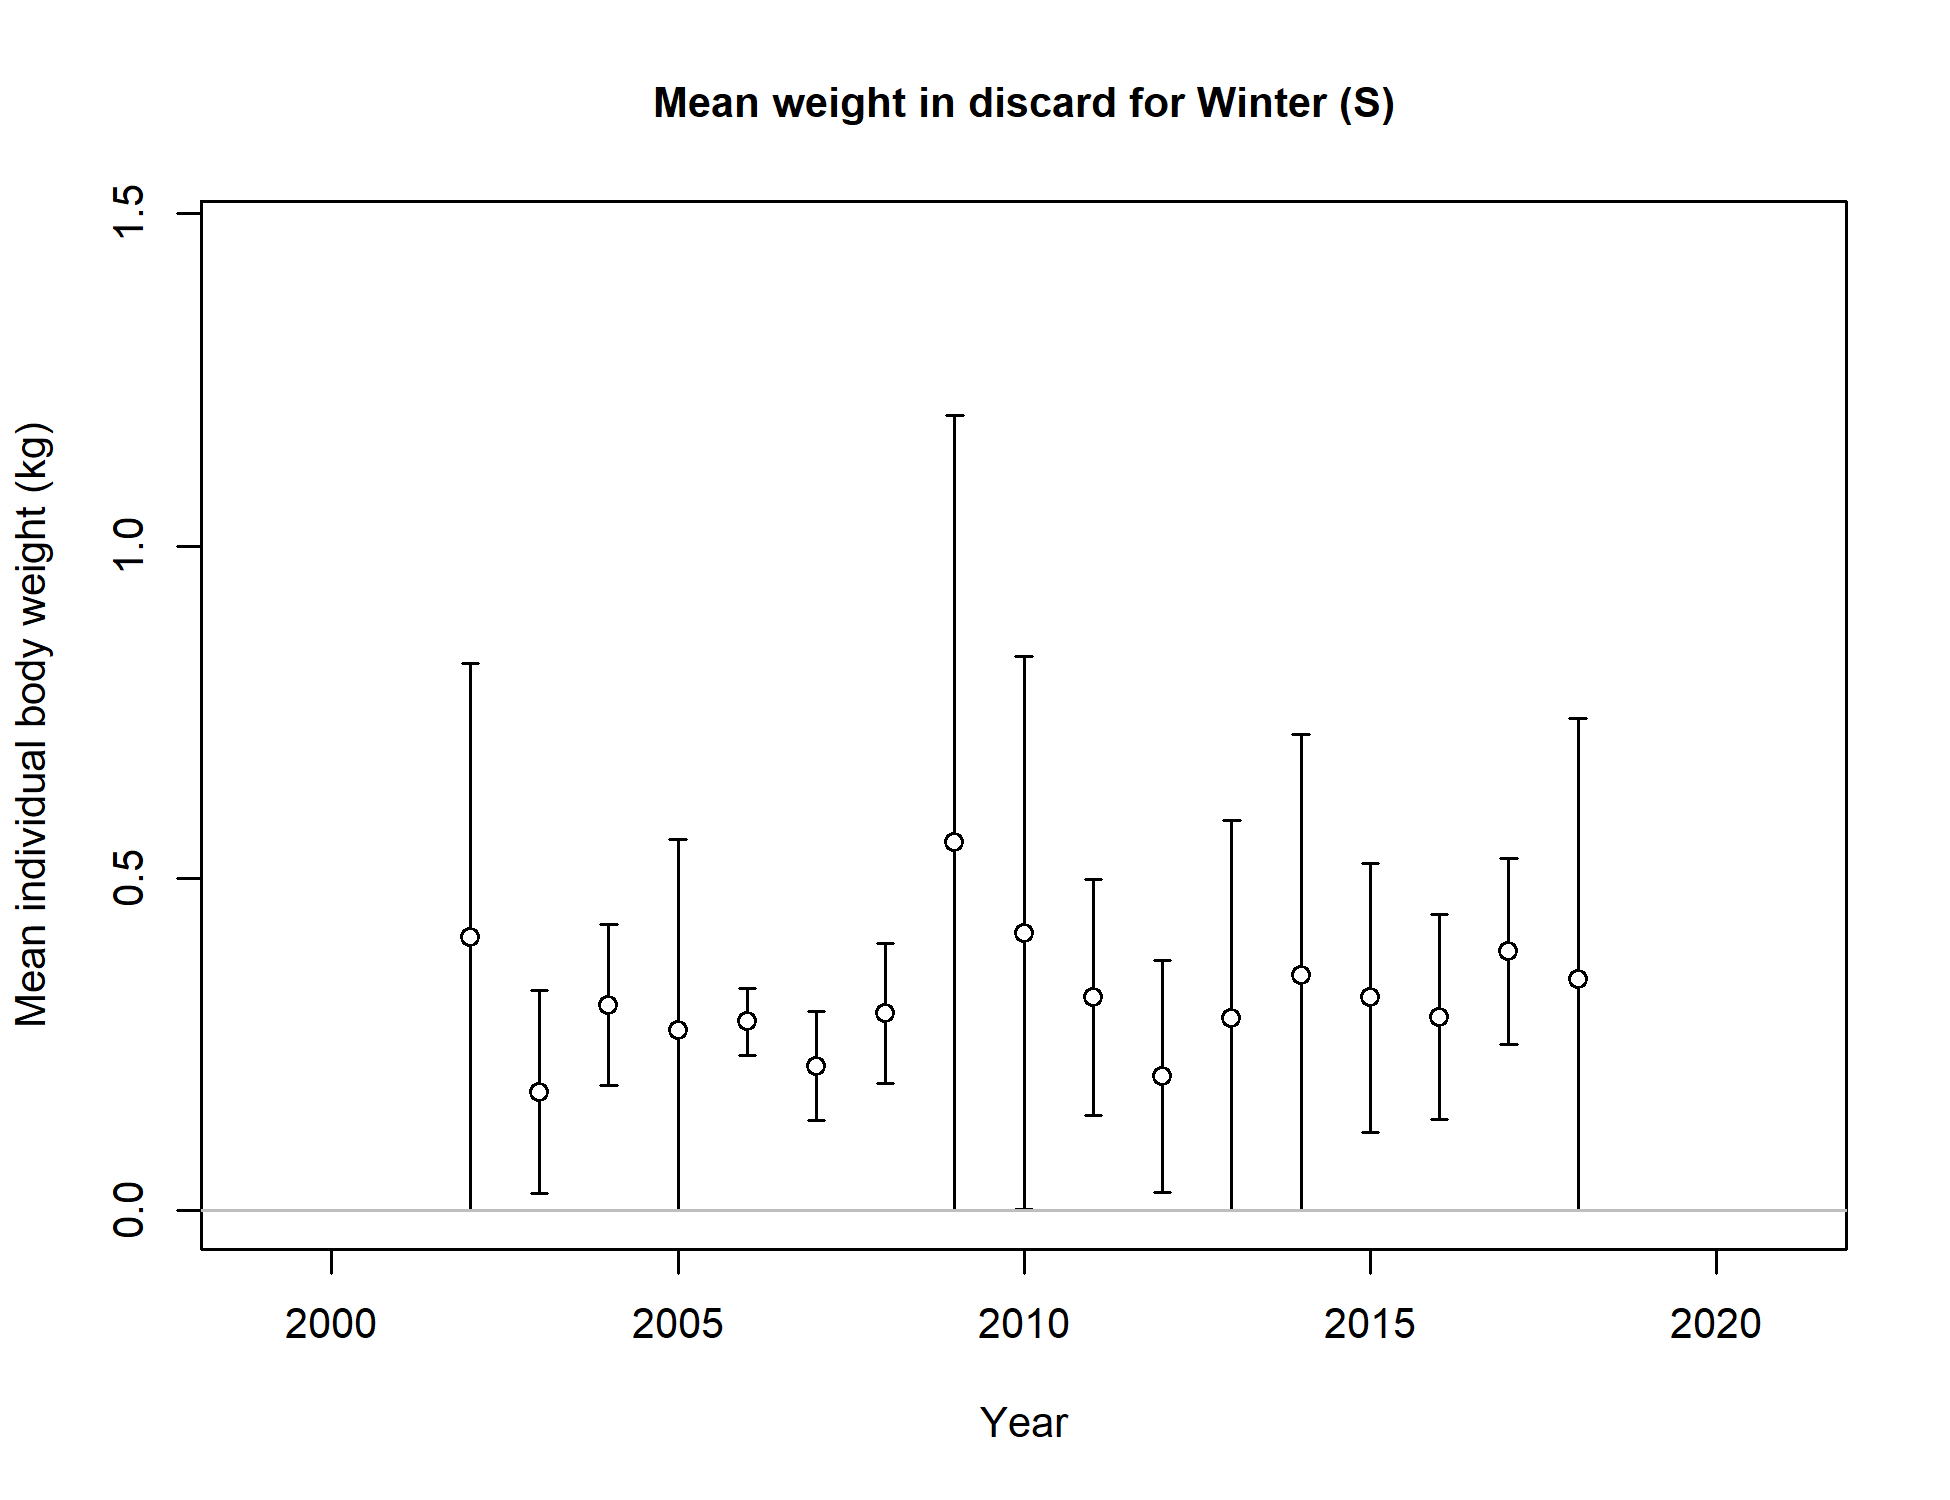
\includegraphics{r4ss/plots_mod1/bodywt_data_fltWinter (S).png}
\caption{Southern winter fishery mean body weights of discarded fish for
petrale sole. \label{fig:sw_bodywt}}
\end{figure}

\FloatBarrier

\begin{figure}
\centering
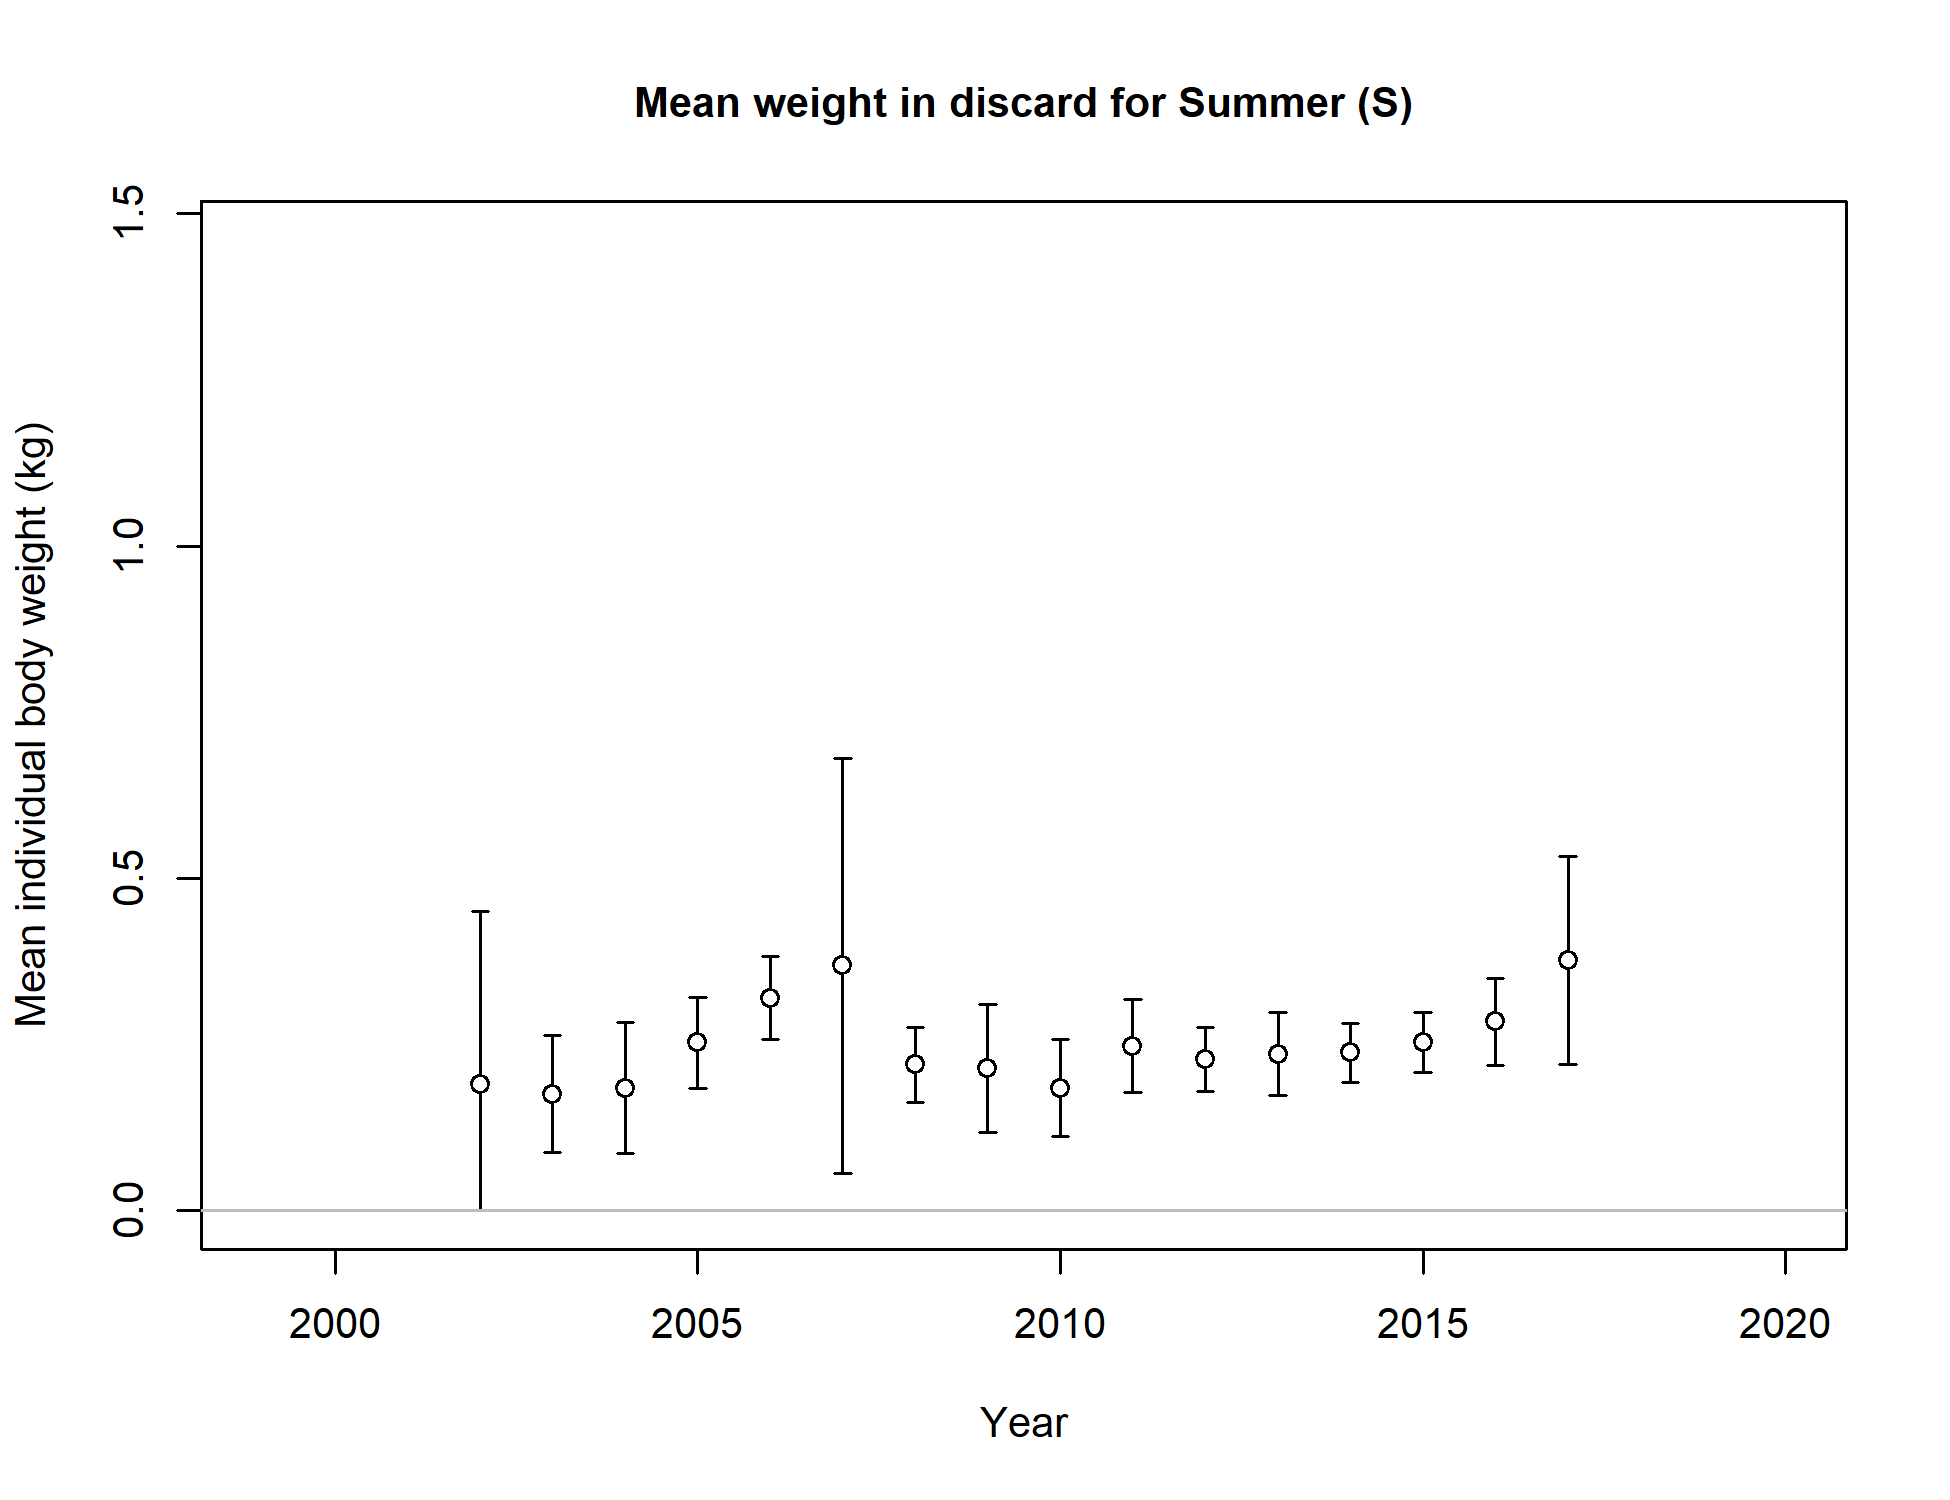
\includegraphics{r4ss/plots_mod1/bodywt_data_fltSummer (S).png}
\caption{Southern summer fishery mean body weights of discarded fish for
petrale sole. \label{fig:ss_bodywt}}
\end{figure}

\FloatBarrier

\begin{figure}
\centering
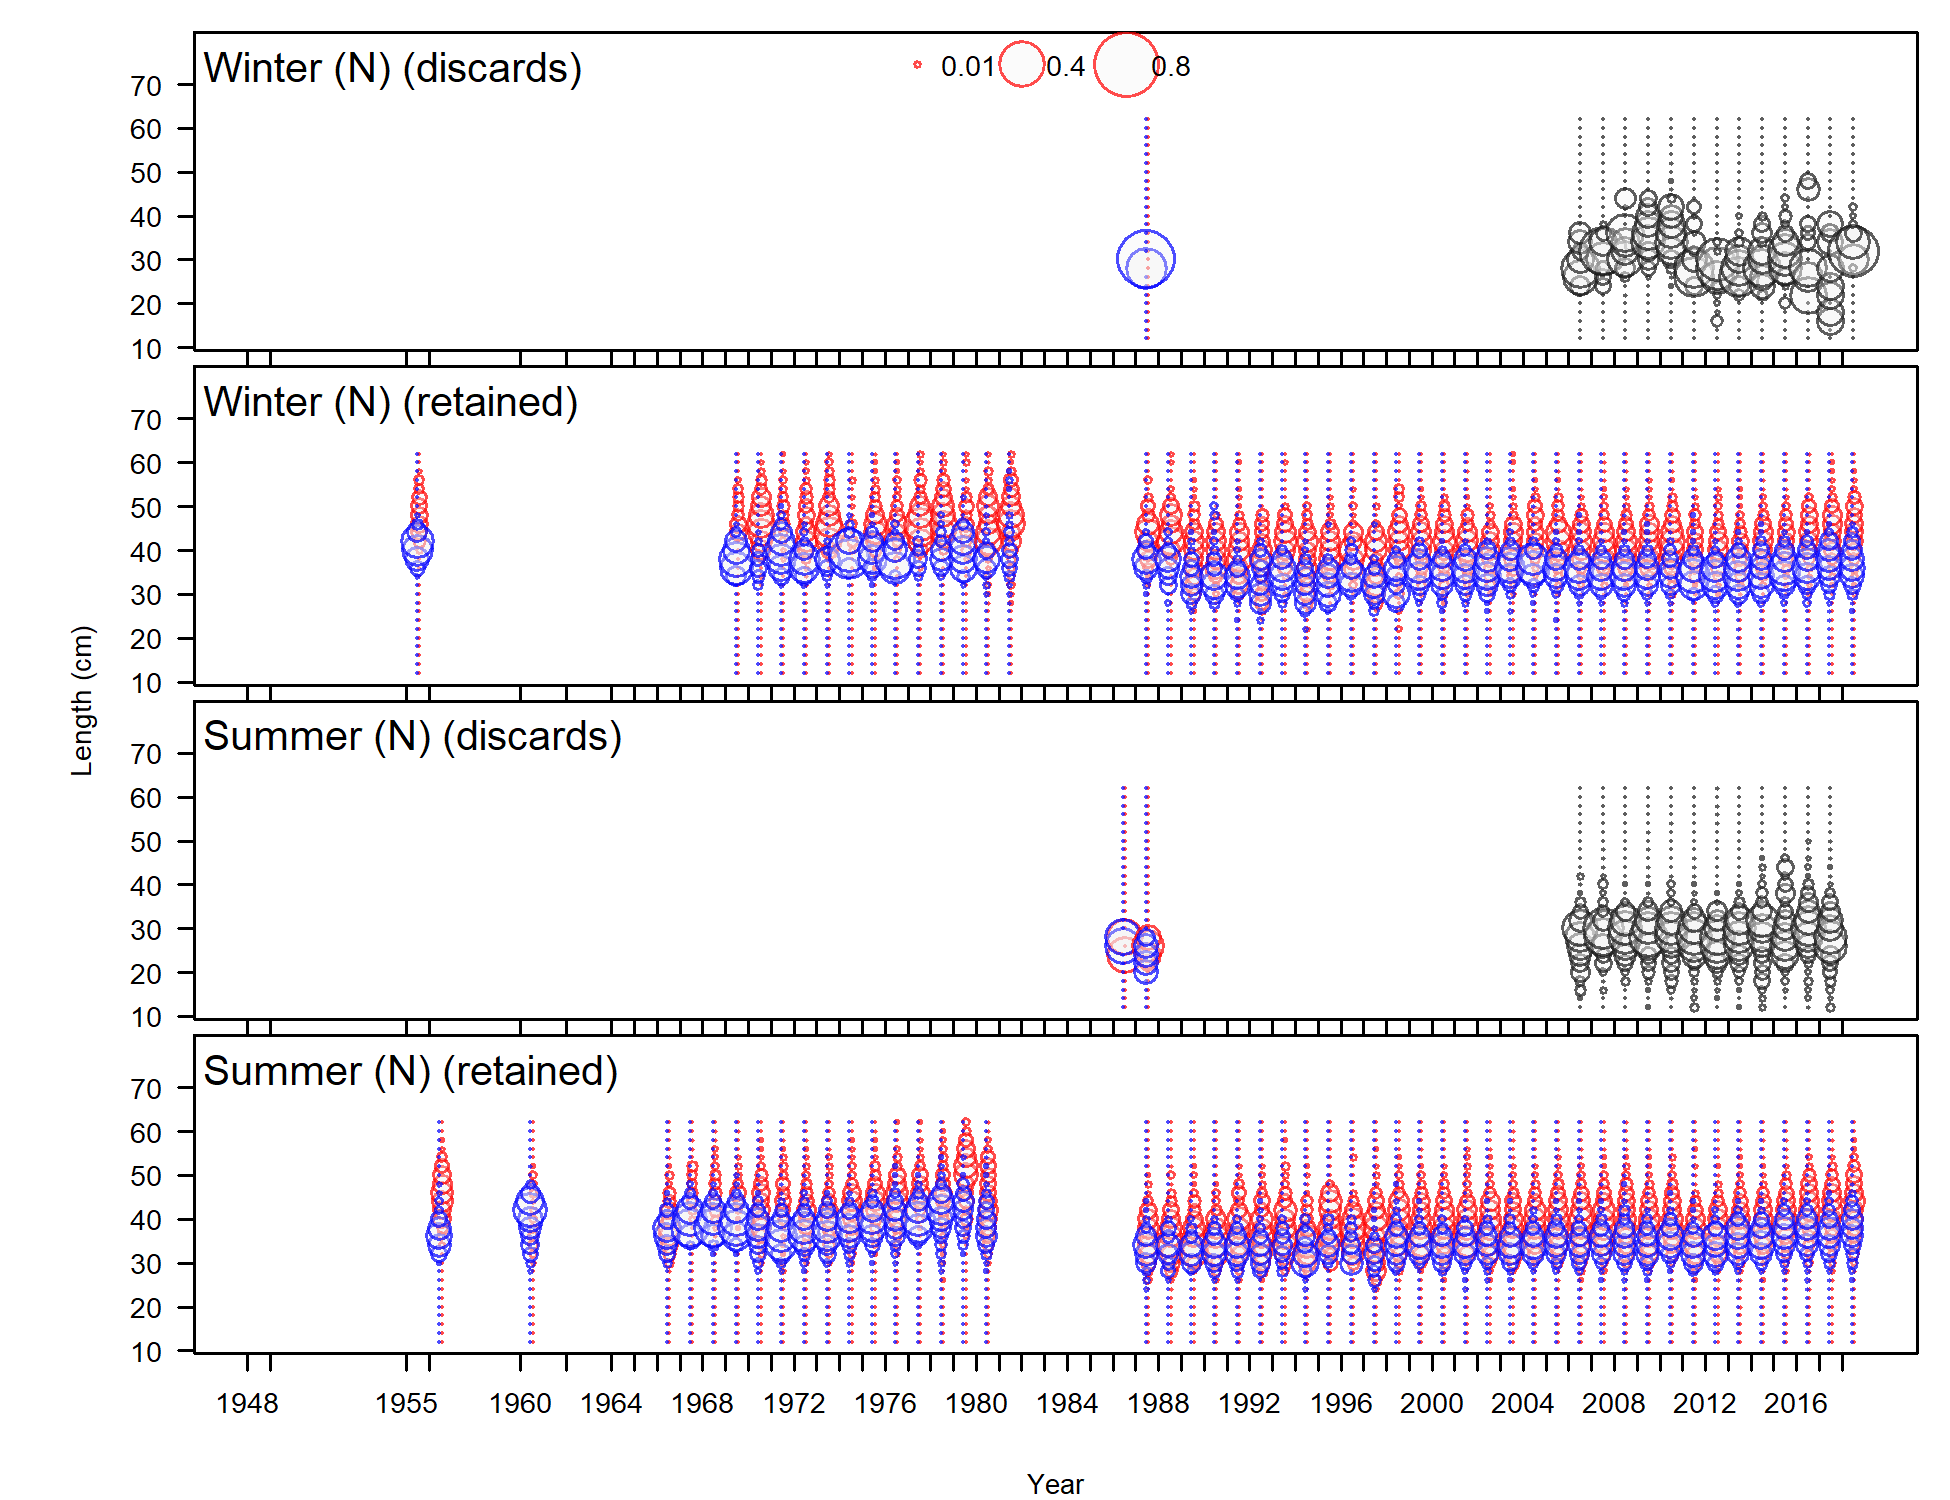
\includegraphics{r4ss/plots_mod1/comp_lendat__page1_multi-fleet_comparison.png}
\caption{Northern fishery, winter and summer, retained and discarded
length frequency distributions for petrale sole.
\label{fig:north_lengths}}
\end{figure}

\FloatBarrier

\begin{figure}
\centering
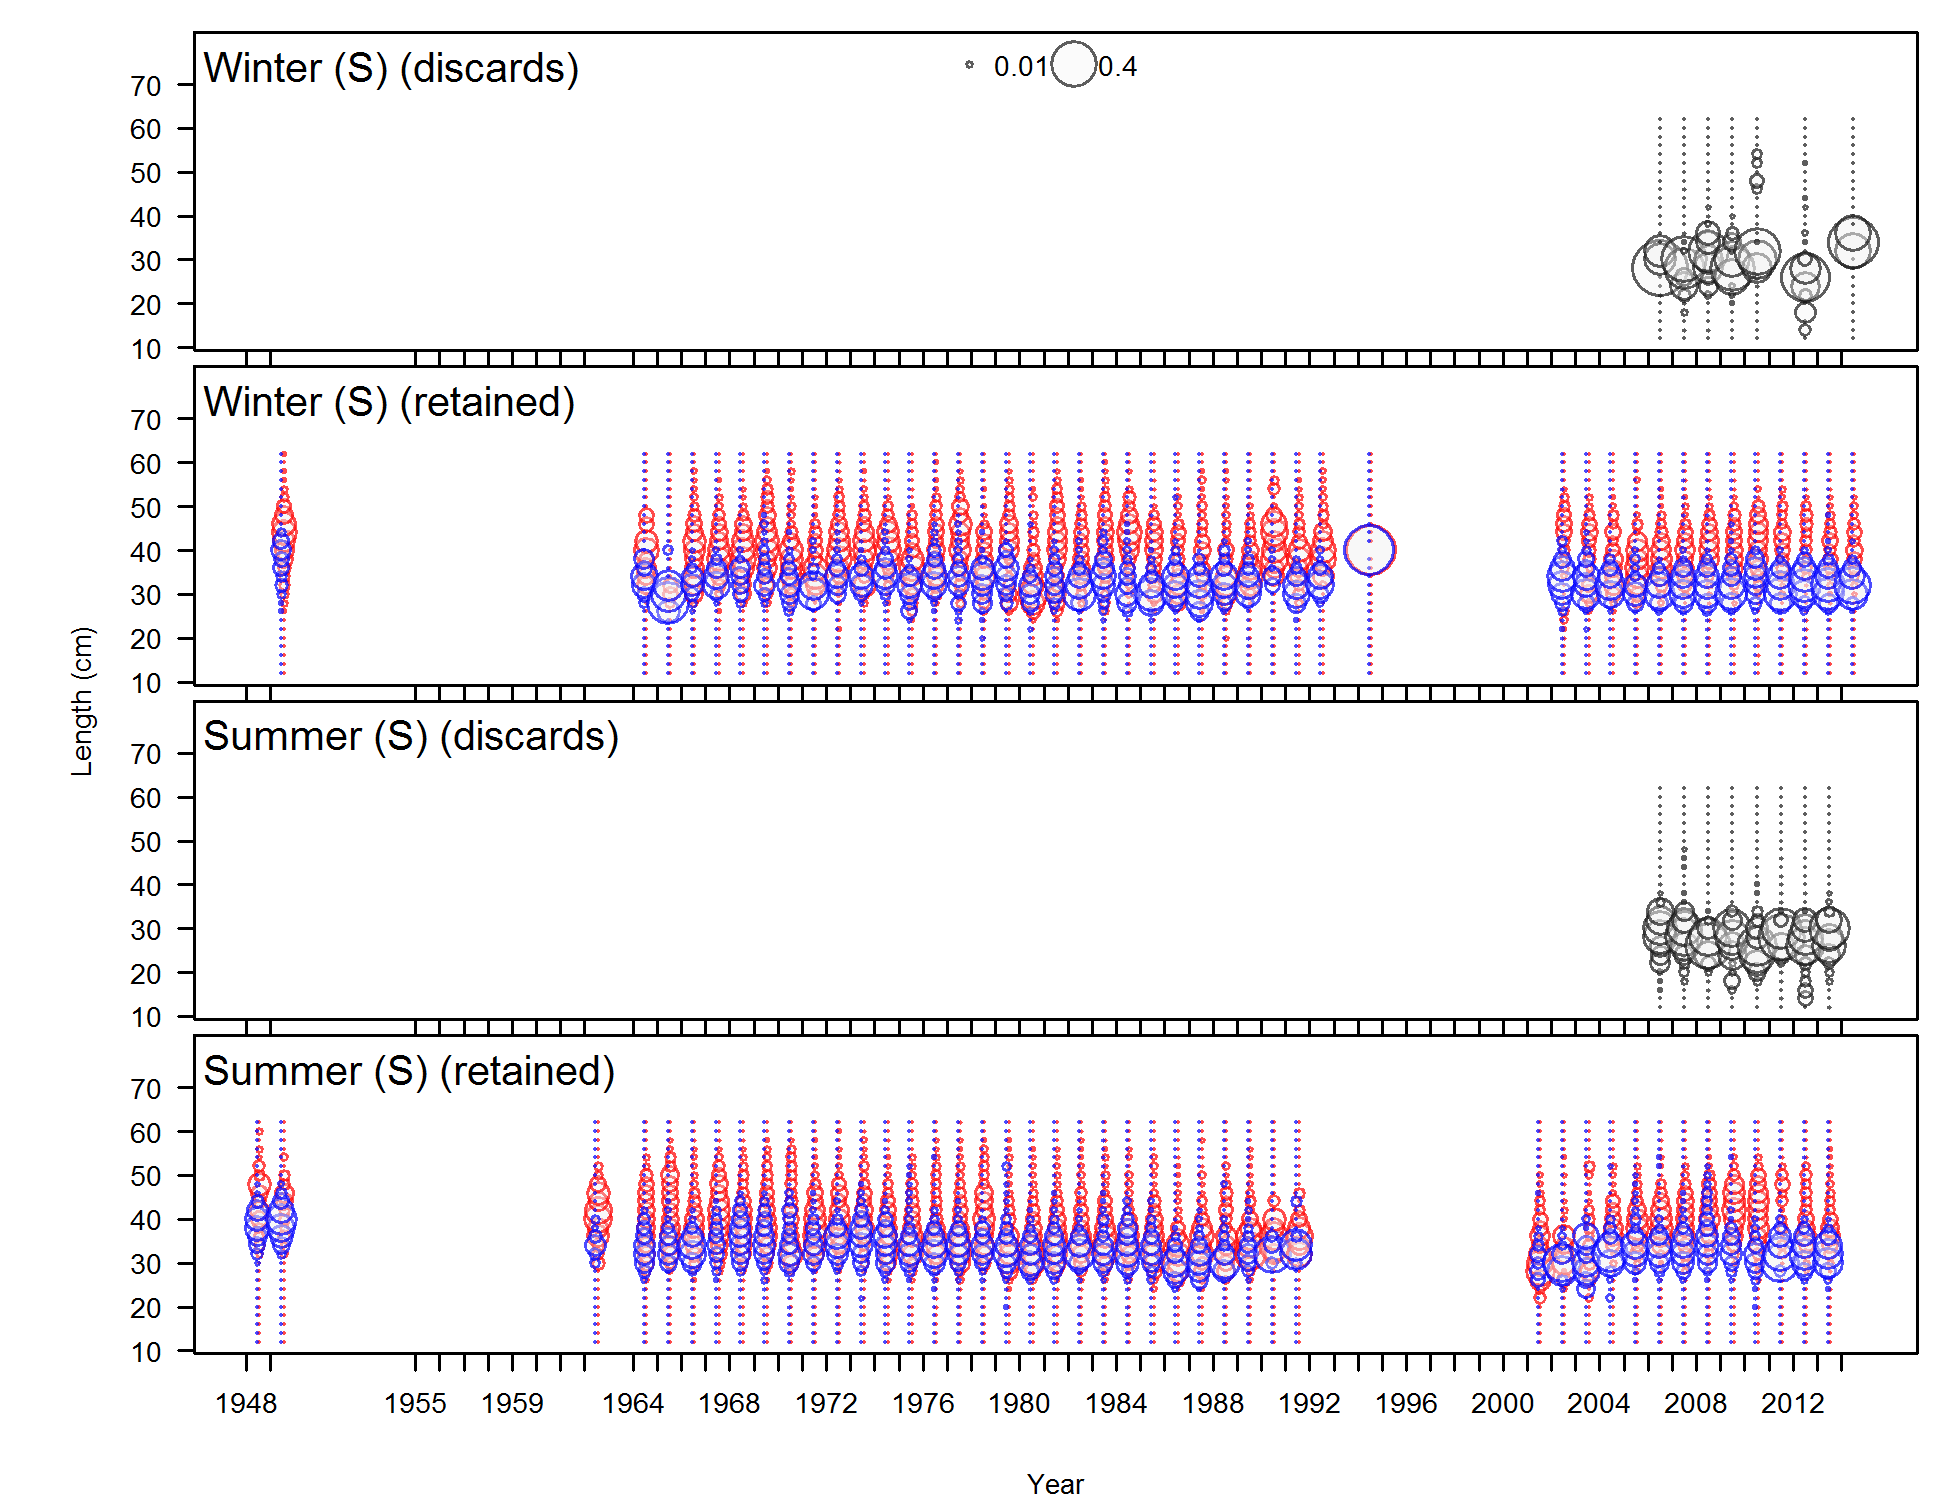
\includegraphics{r4ss/plots_mod1/comp_lendat__page2_multi-fleet_comparison.png}
\caption{Southern fishery, winter and summer, retained and discarded
length frequency distributions for petrale sole.
\label{fig:south_lengths}}
\end{figure}

\FloatBarrier

\begin{figure}
\centering
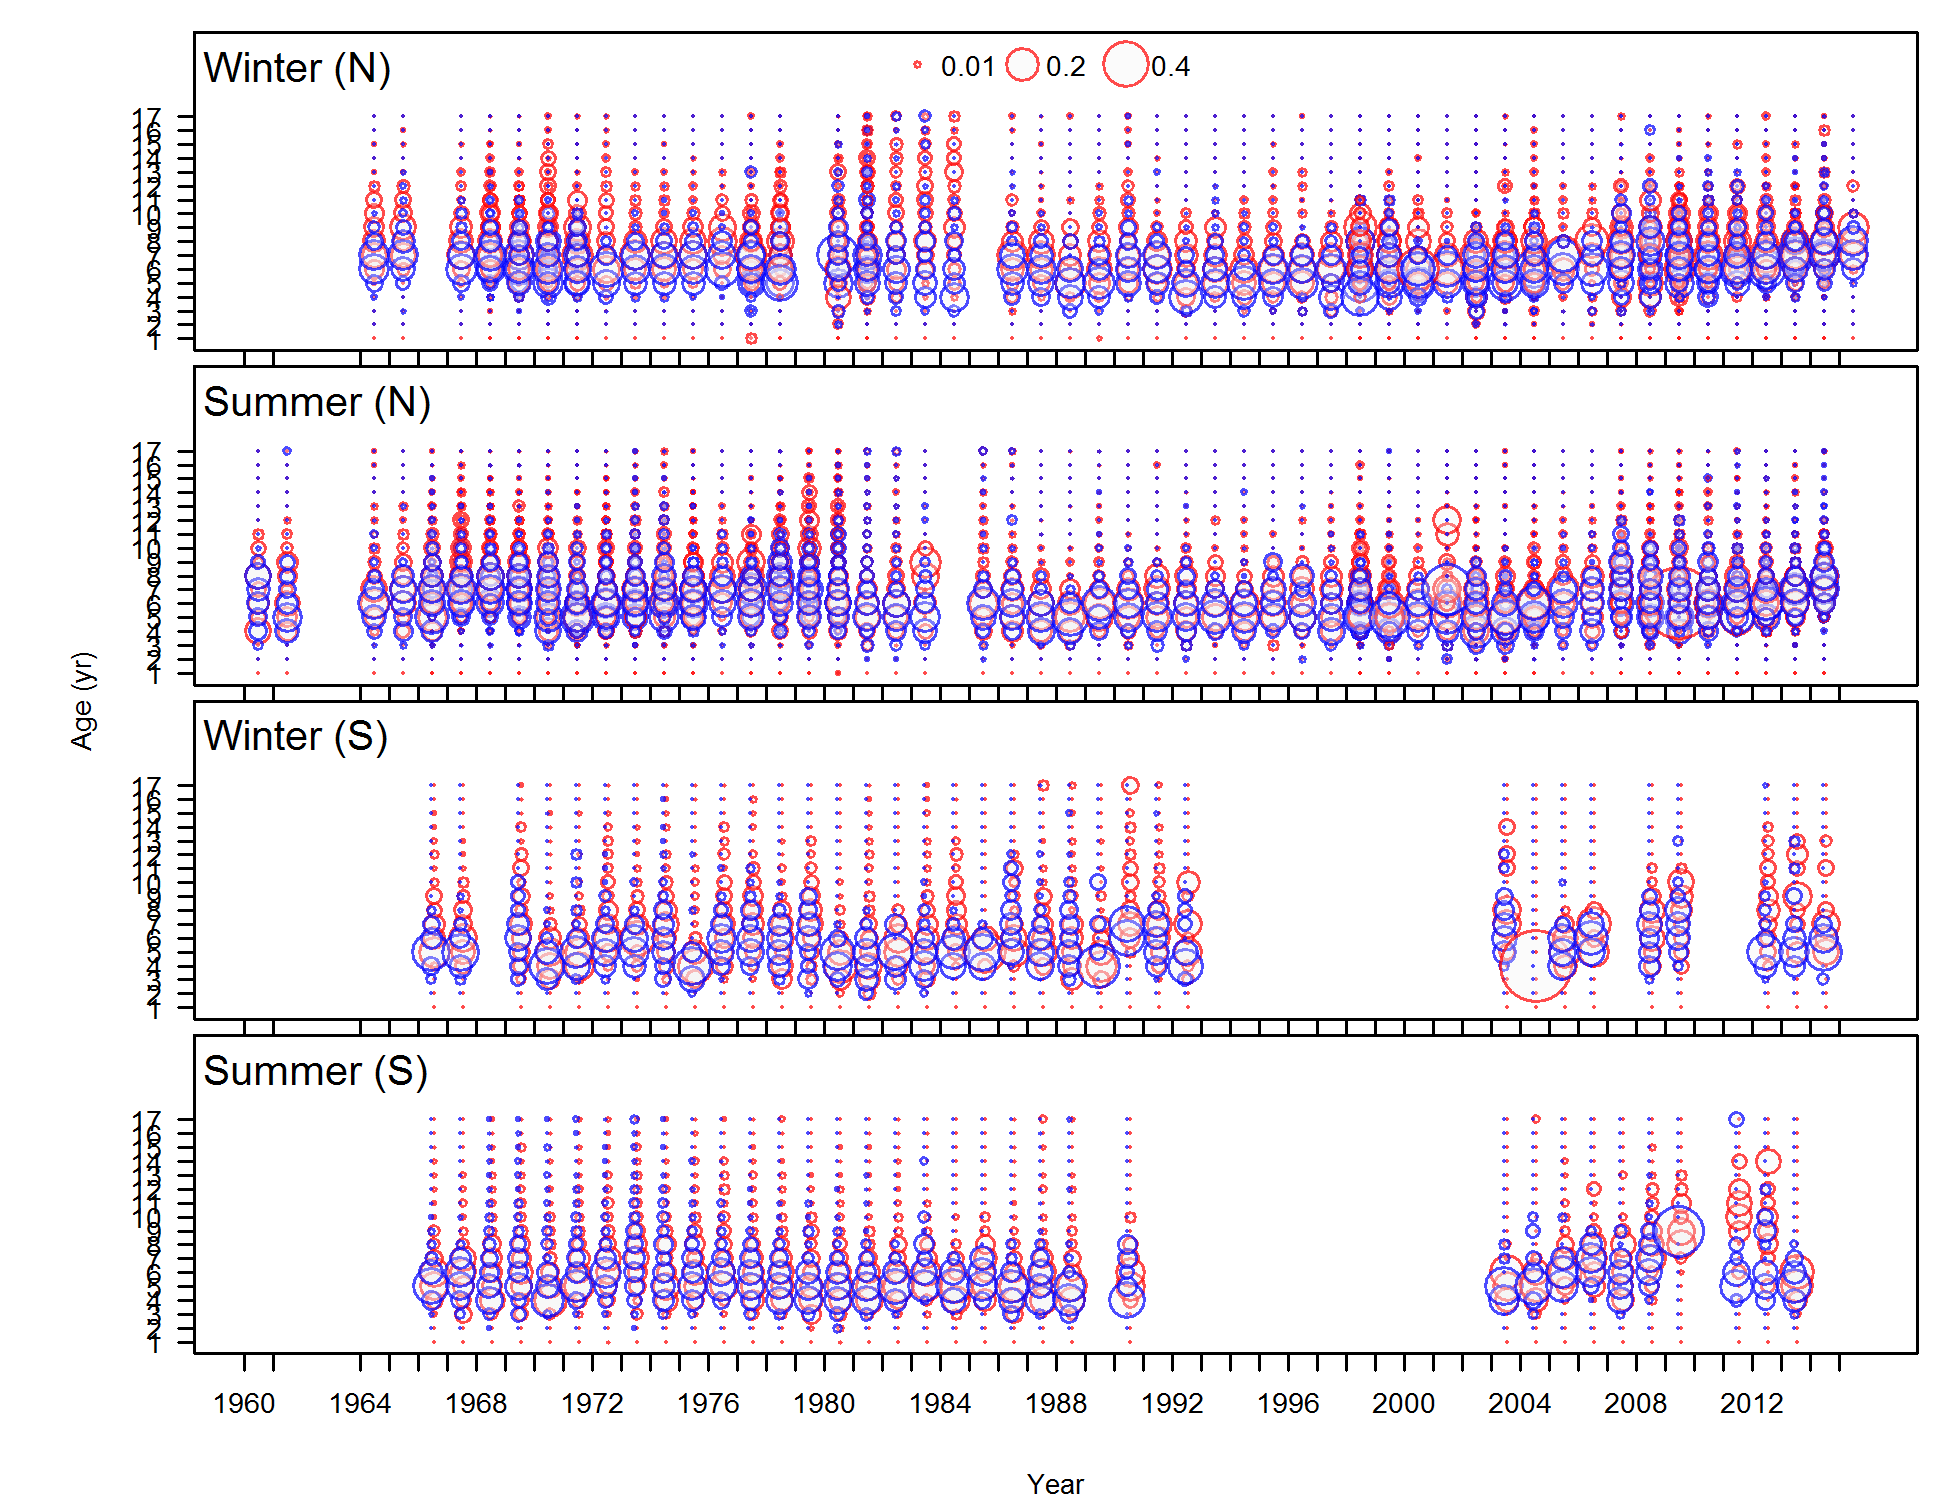
\includegraphics{r4ss/plots_mod1/comp_agedat__multi-fleet_comparison.png}
\caption{Commercial fishery age frequency distributions for petrale
sole. \label{fig:comm_ages}}
\end{figure}

\FloatBarrier

\begin{figure}
\centering
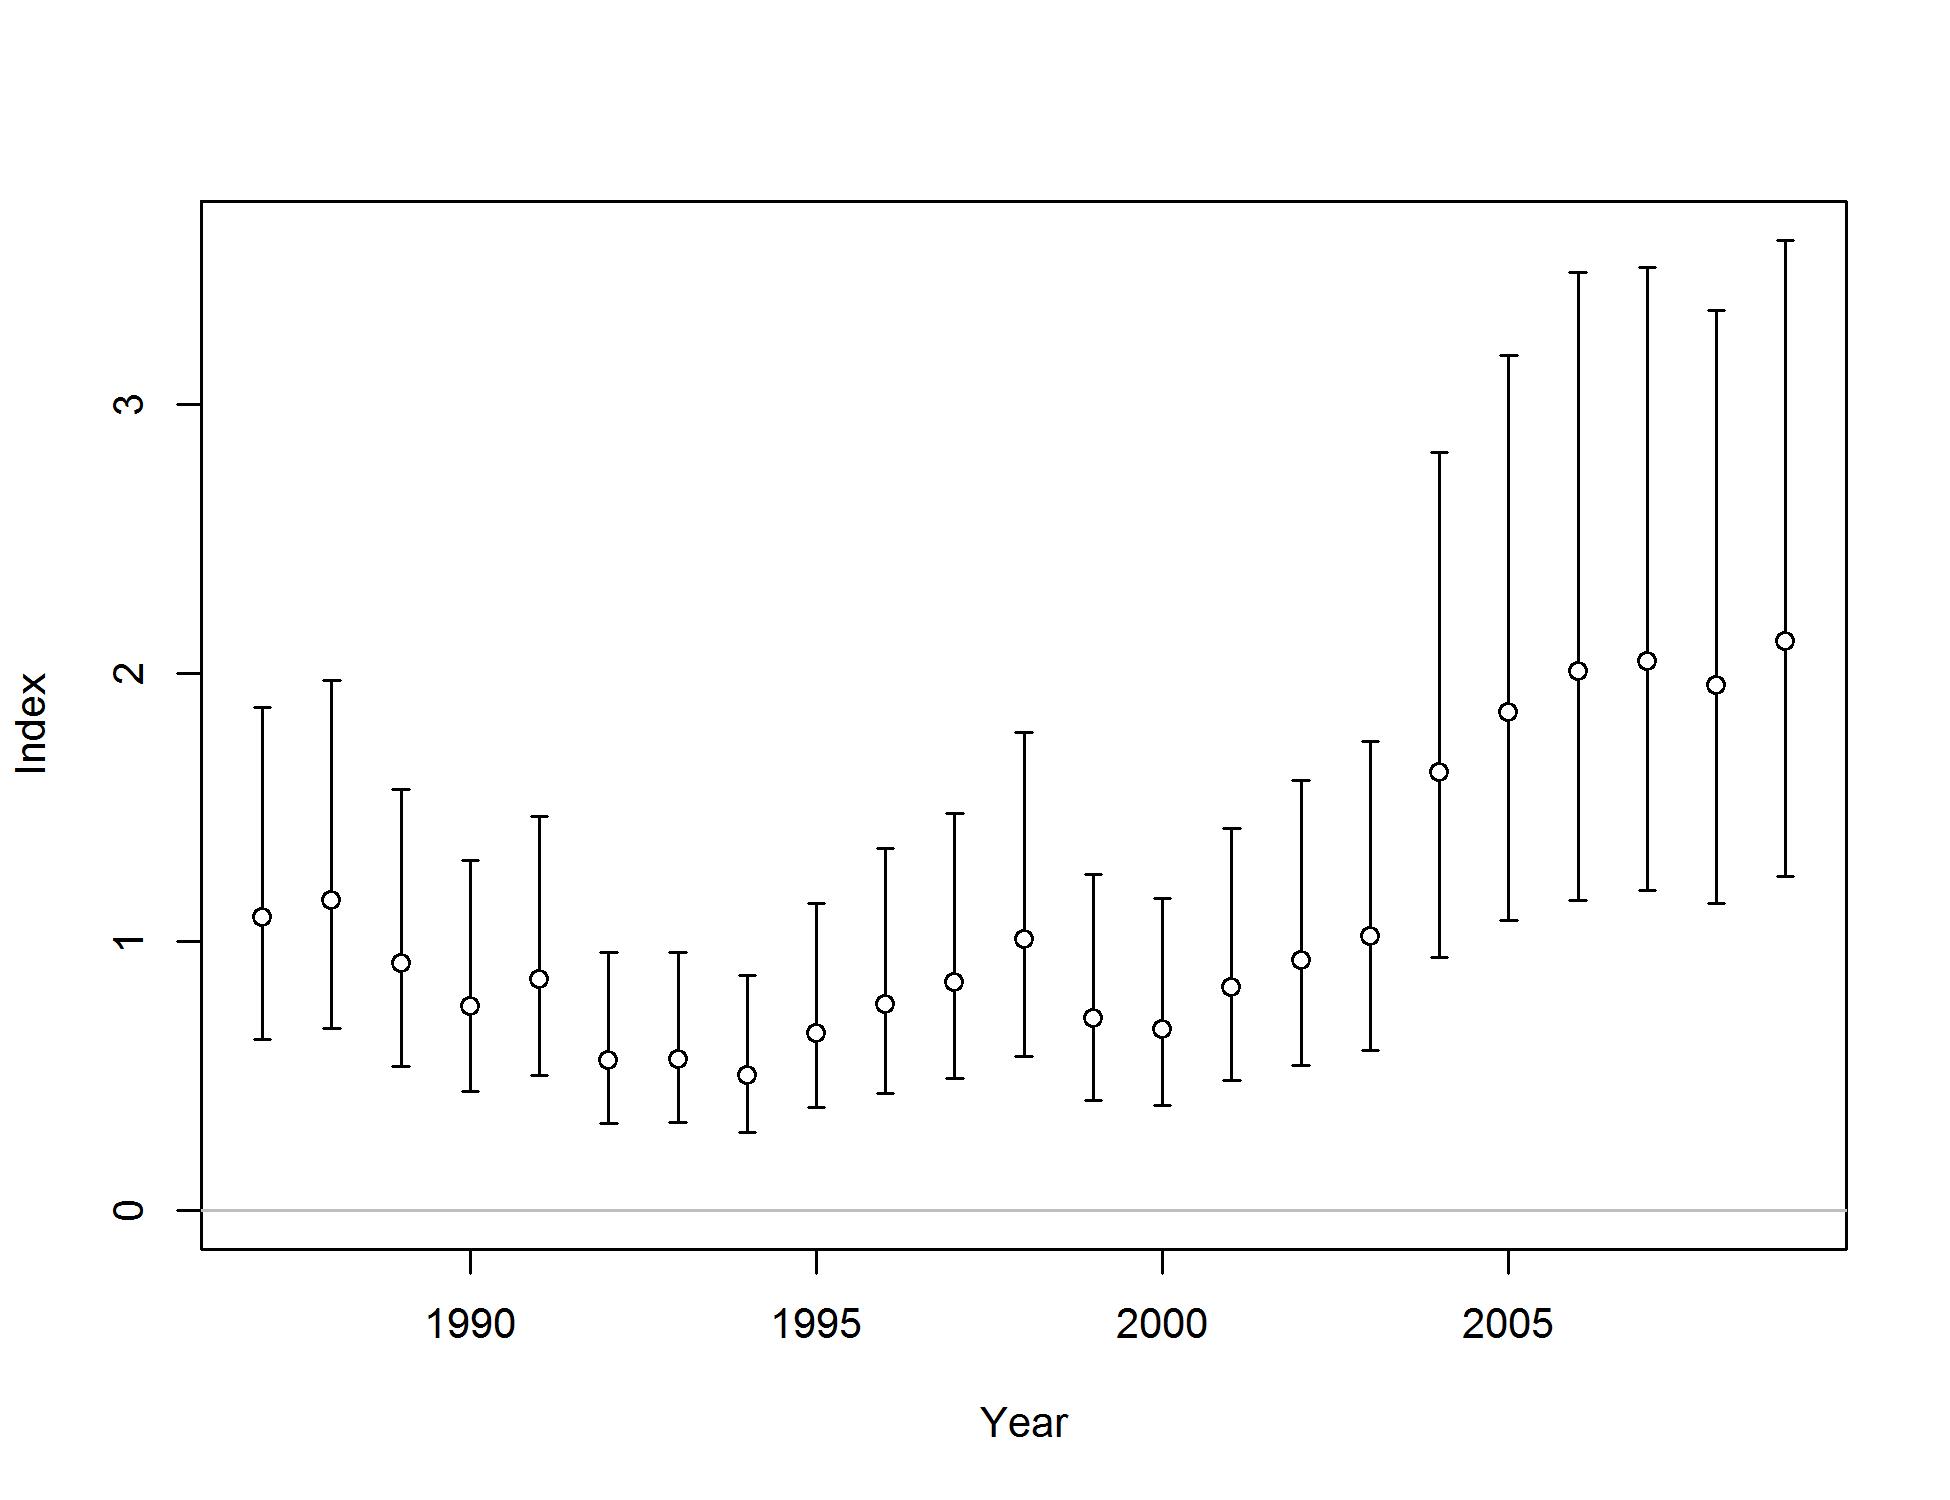
\includegraphics{r4ss/plots_mod1/index1_cpuedata_Winter (N).png}
\caption{The Northern Winter fishery catch-per-unit-effort based on
logbook data for petrale sole. \label{fig:north_cpue}}
\end{figure}

\FloatBarrier

\begin{figure}
\centering
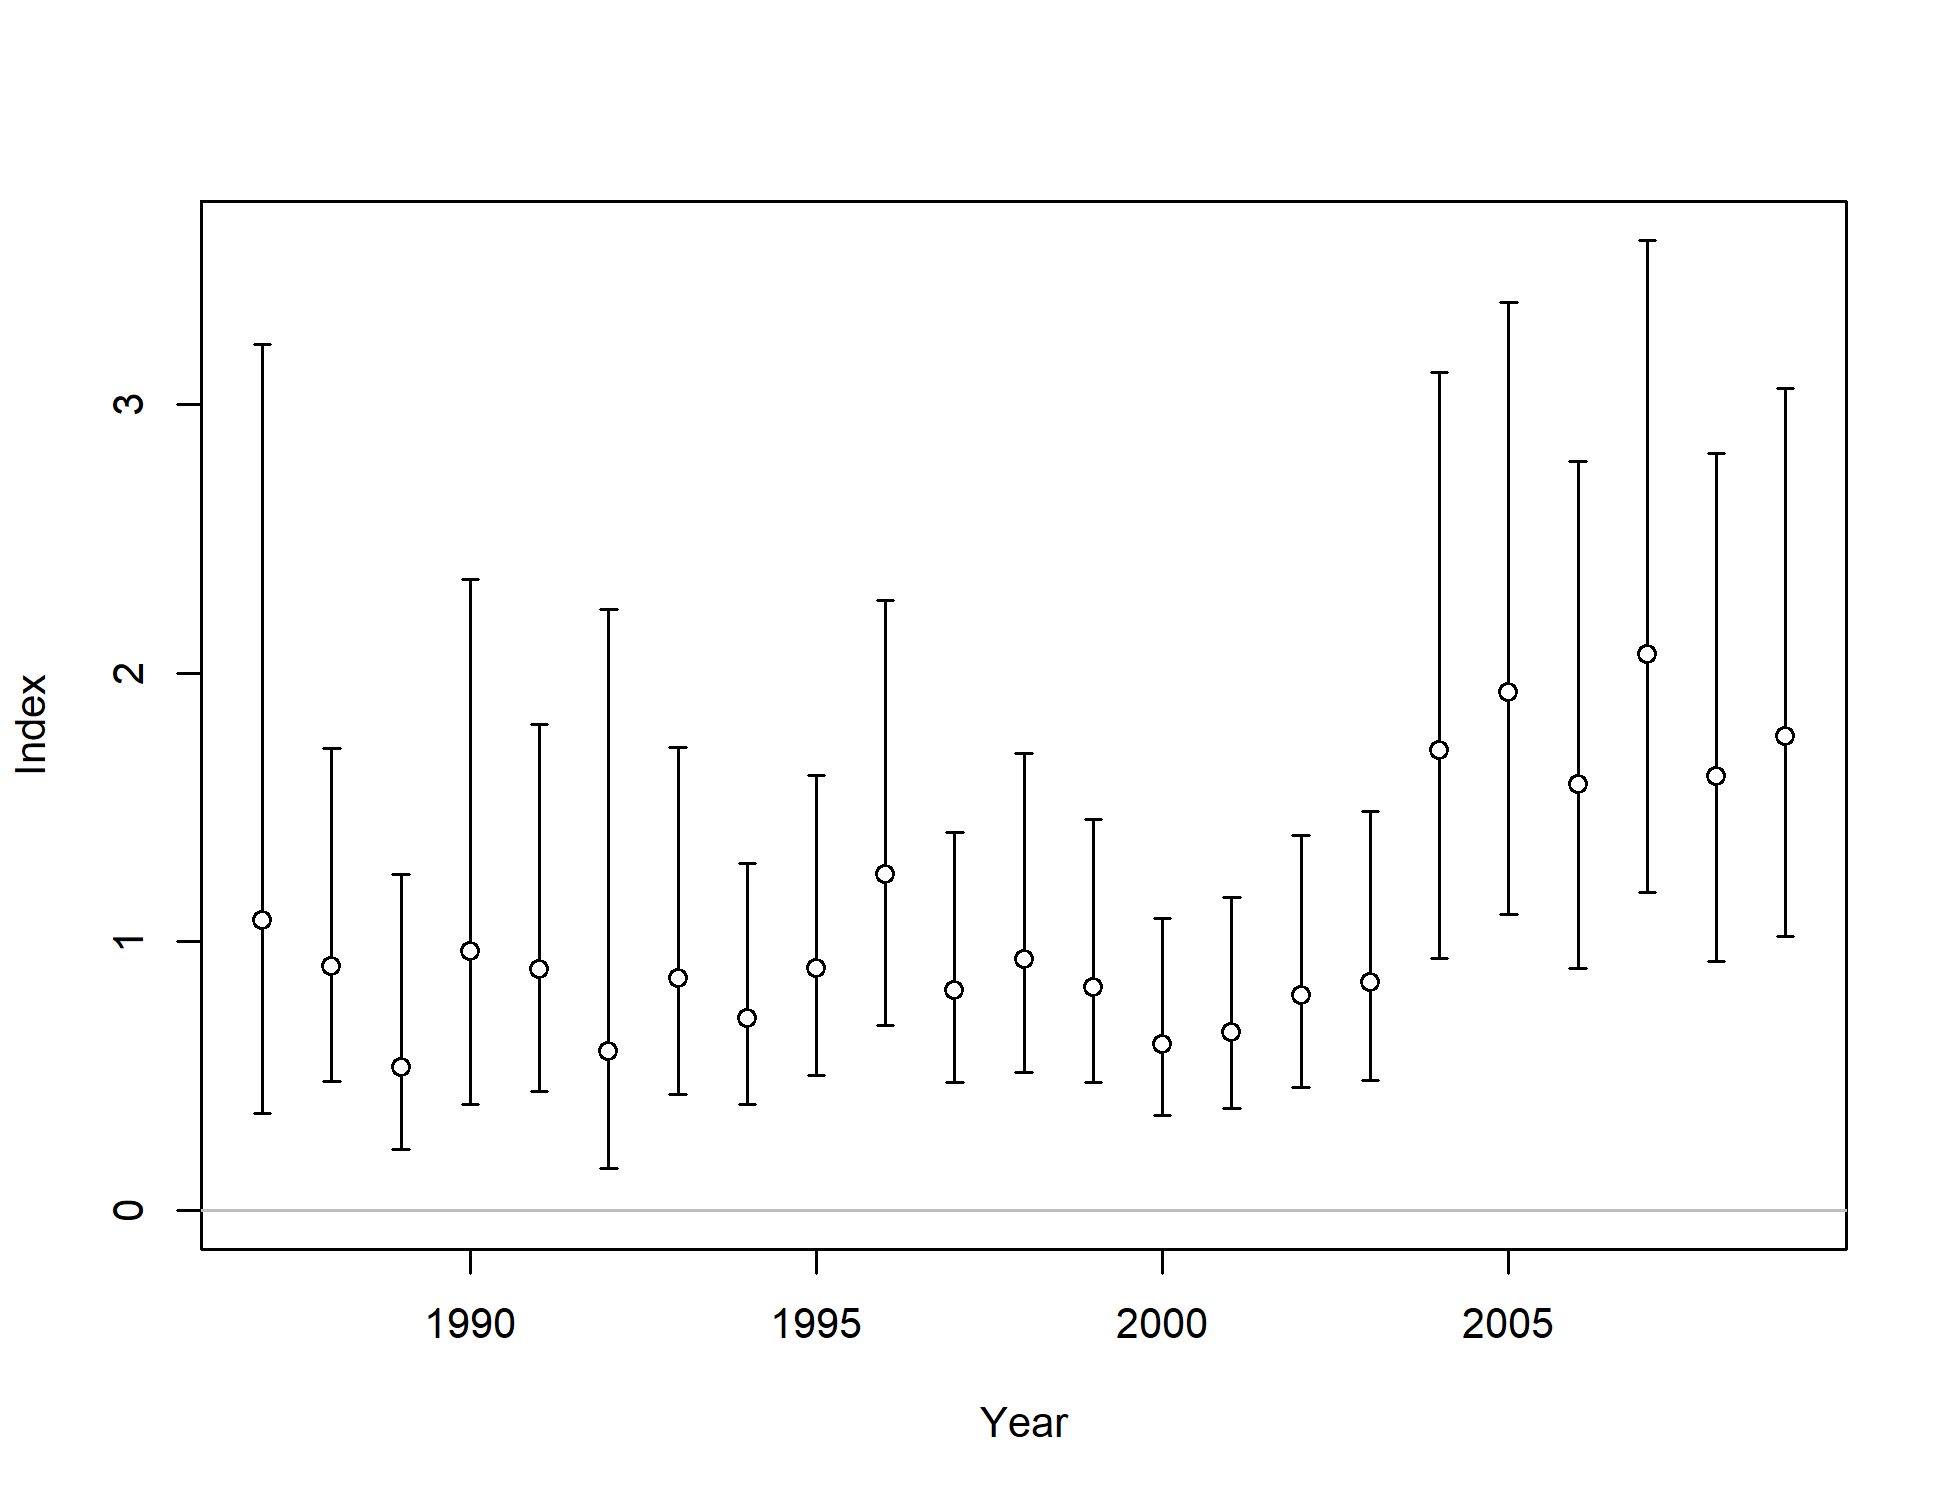
\includegraphics{r4ss/plots_mod1/index1_cpuedata_Winter (S).png}
\caption{The Southern Winter fishery catch-per-unit-effort based on
logbook data for petrale sole. \label{fig:south_cpue}}
\end{figure}

\FloatBarrier

\begin{figure}
\centering
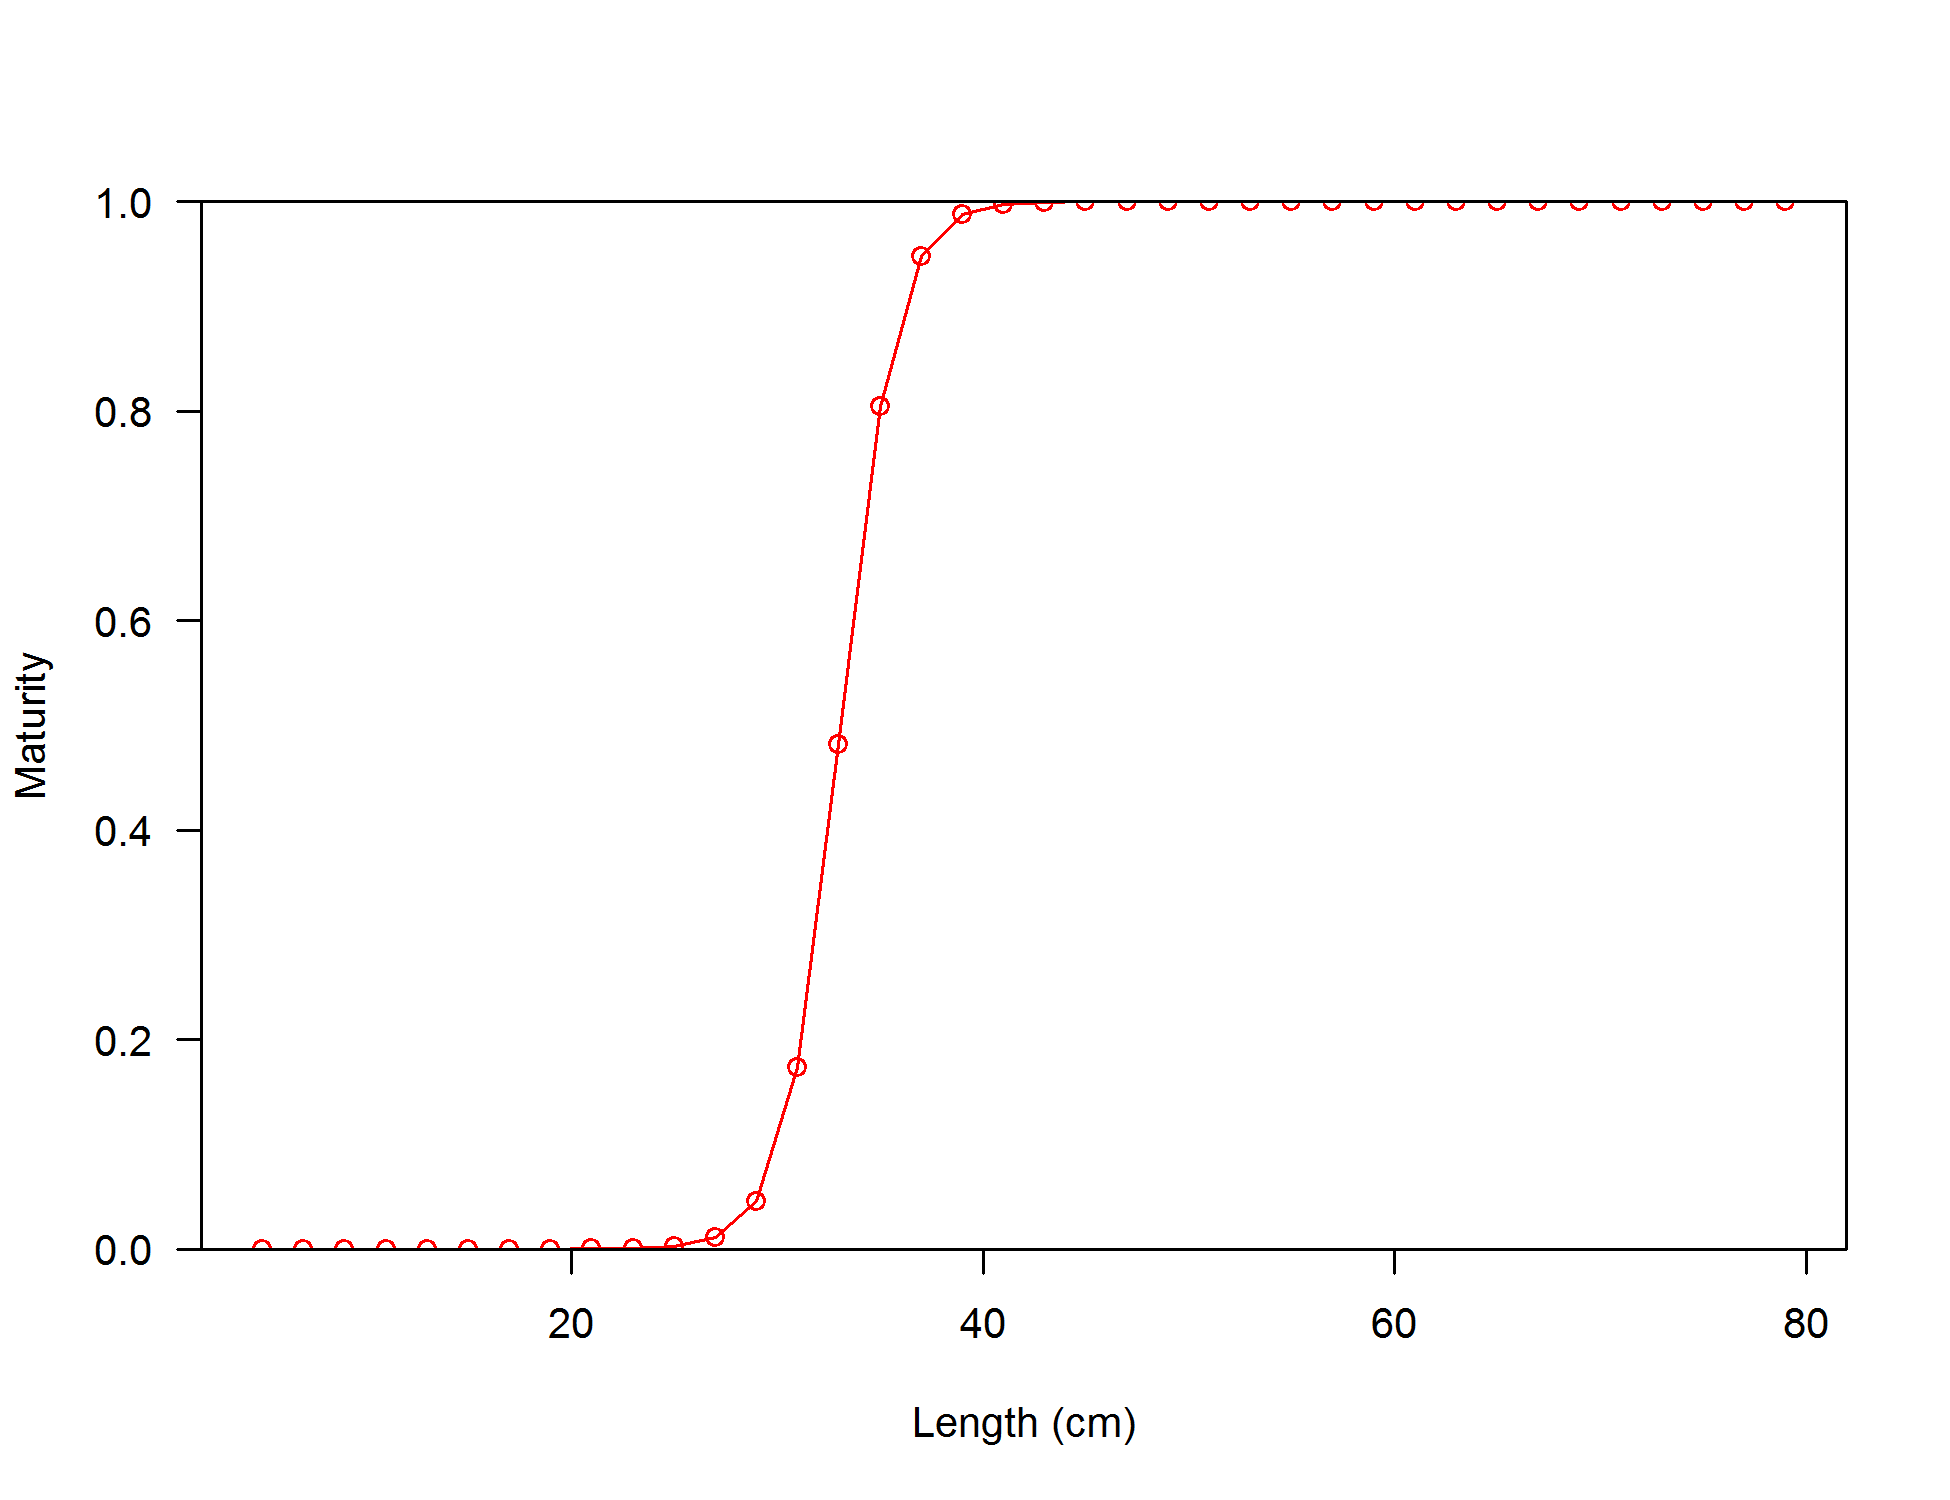
\includegraphics{r4ss/plots_mod1/bio6_maturity.png}
\caption{Estimated maturity-at-length for petrale sole.
\label{fig:maturity}}
\end{figure}

\FloatBarrier

\begin{figure}
\centering
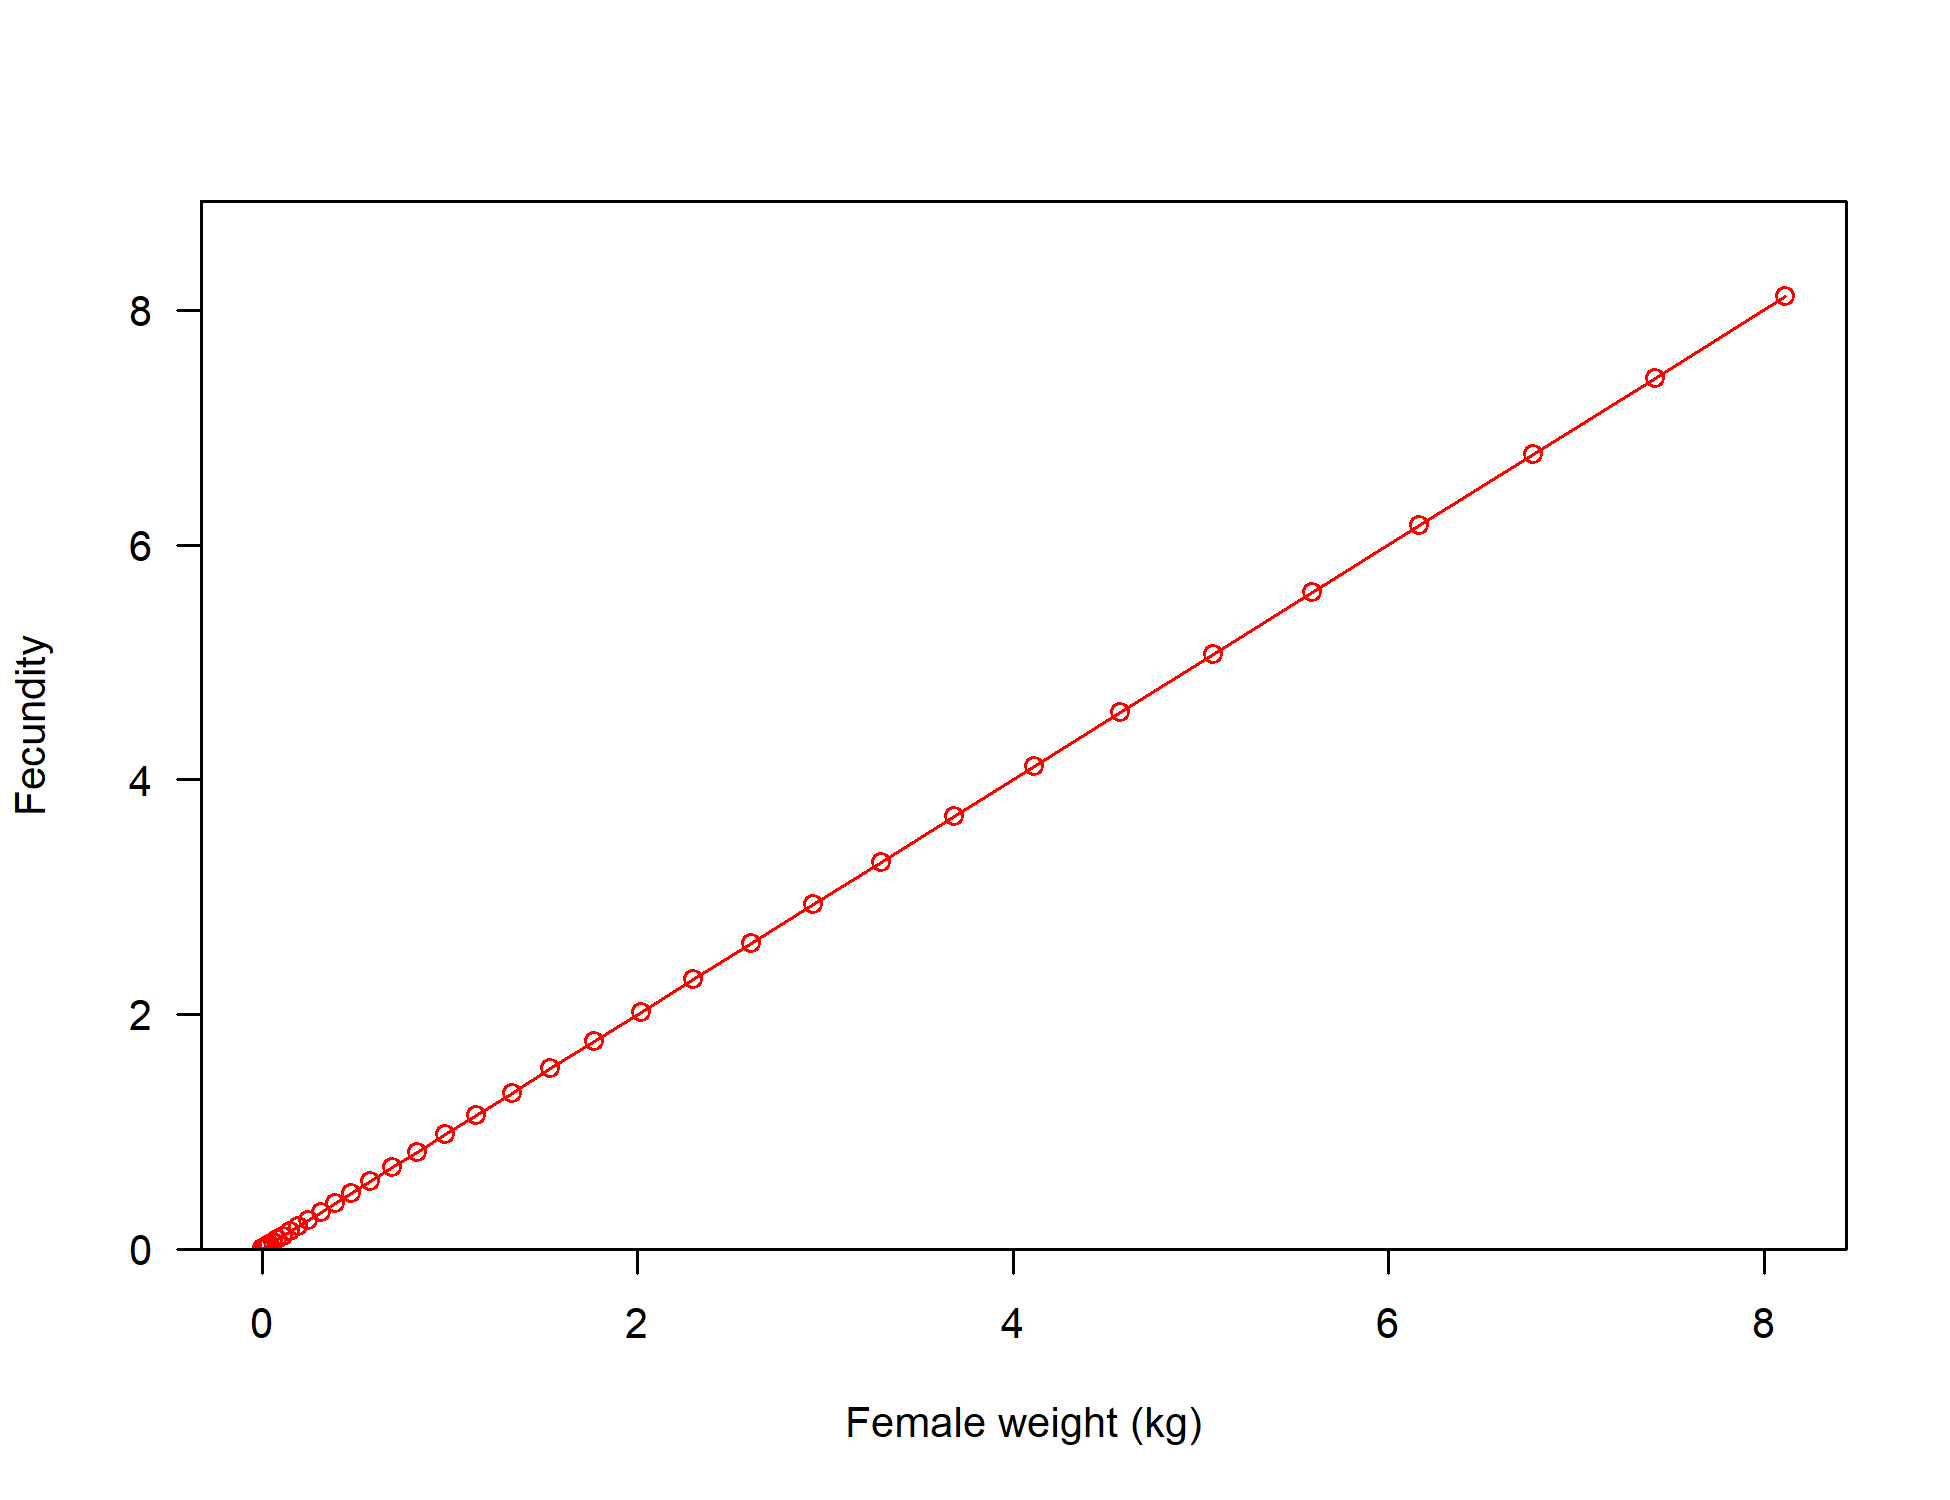
\includegraphics{r4ss/plots_mod1/bio8_fecundity_wt.png}
\caption{Fecundity-at-length assumed in the model for petrale sole.
\label{fig:fecundity_model}}
\end{figure}

\FloatBarrier

\begin{figure}
\centering
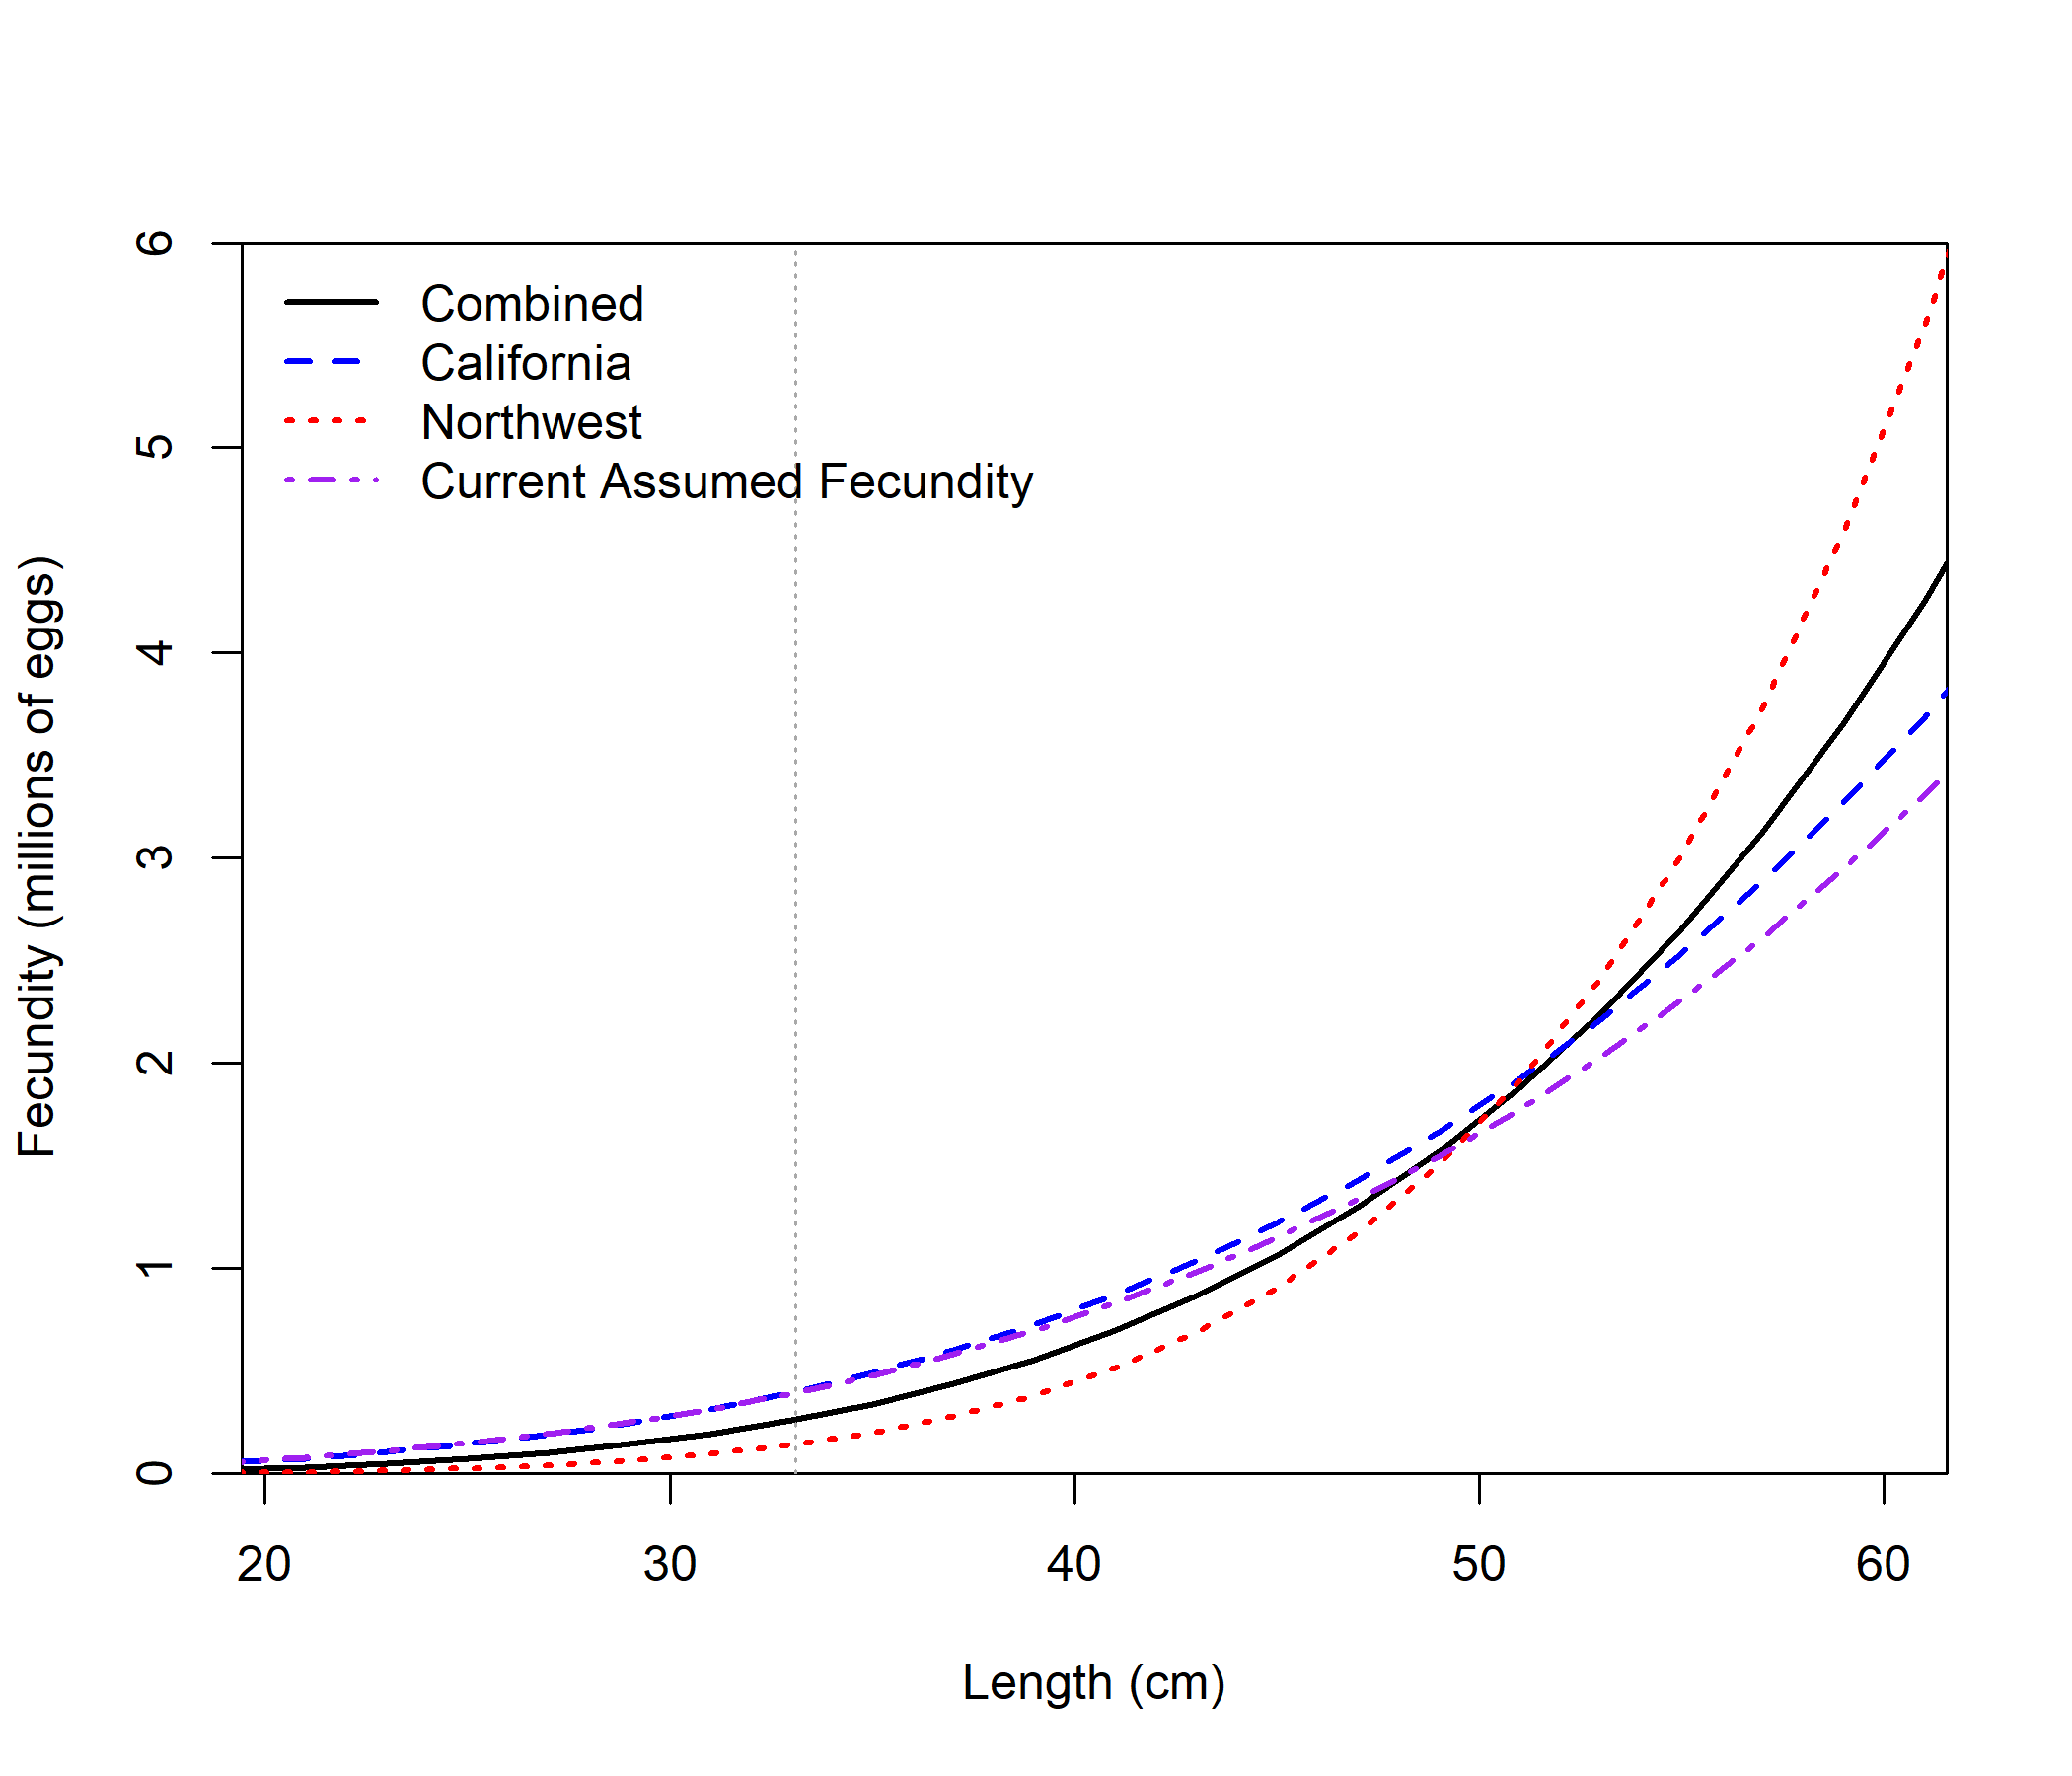
\includegraphics{Figures/fecundity.png}
\caption{Estimated fecundity-at-length for petrale sole based on
Lefebvre et al. (in press). \label{fig:fecundity}}
\end{figure}

\FloatBarrier

\begin{figure}
\centering
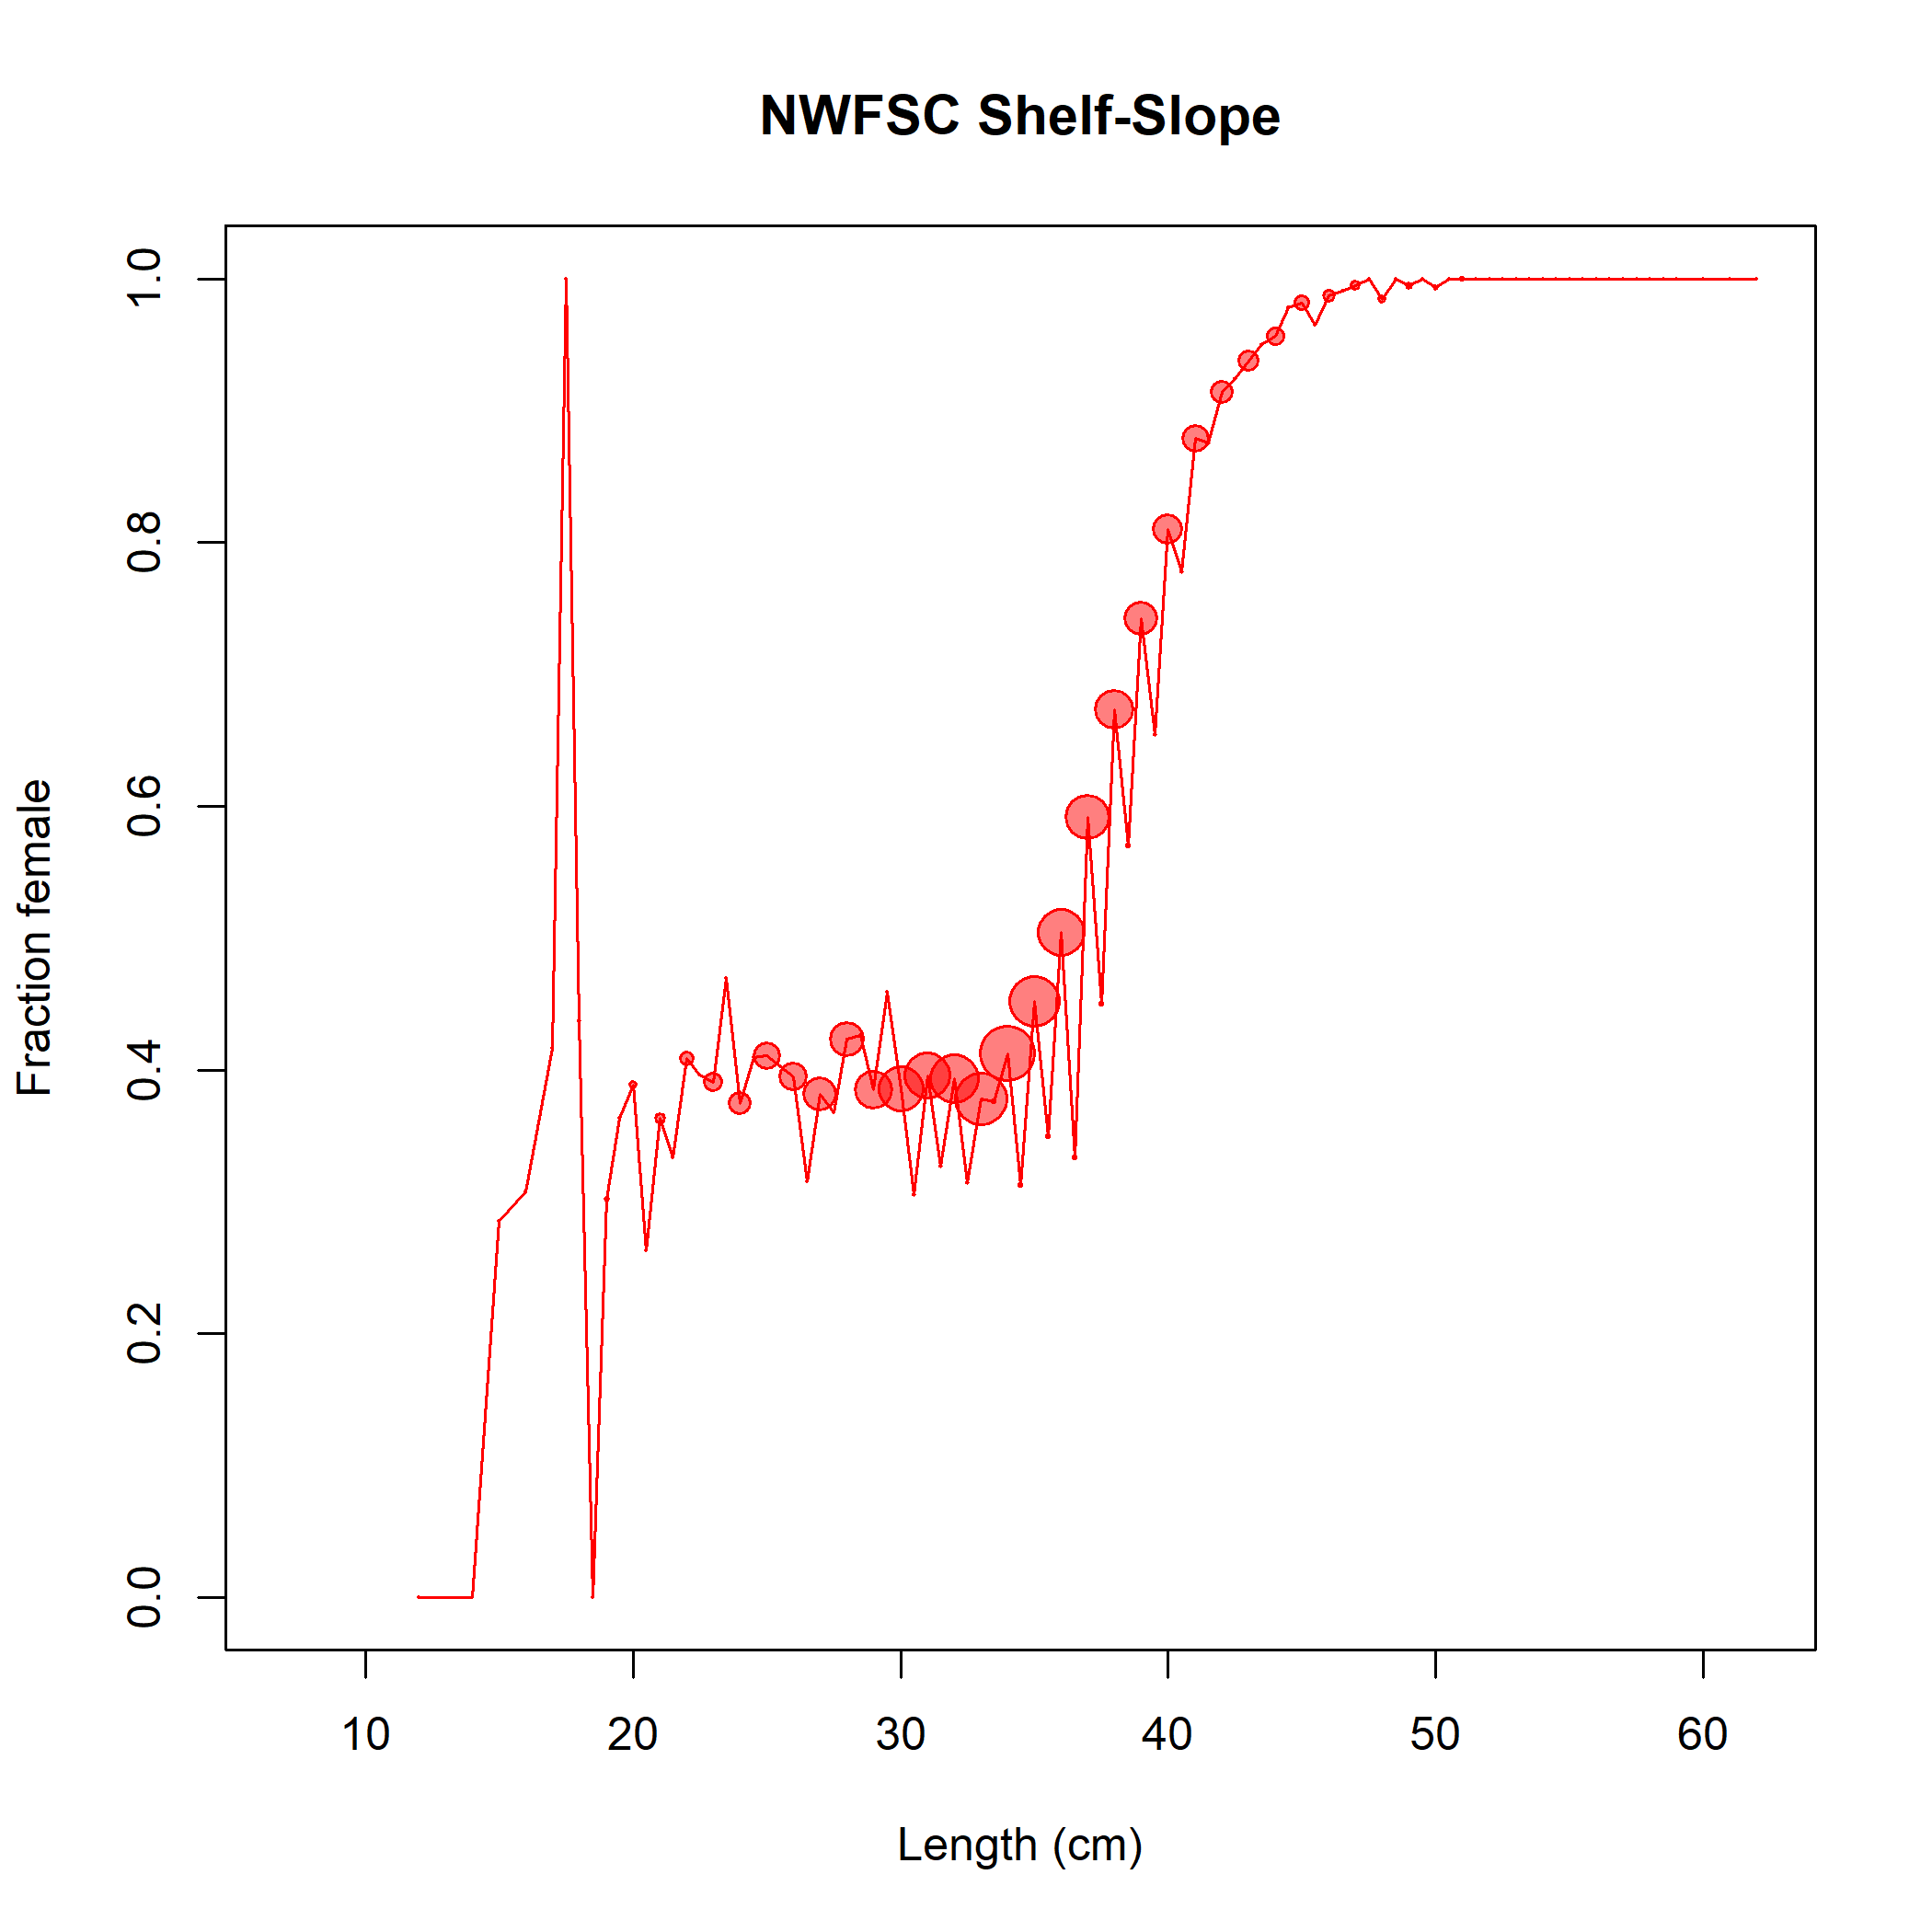
\includegraphics{Figures/NWFSC Shelf-Slope_length_fraction_female.png}
\caption{Estimated proportion of female fish collected by the NWFSC
shelf-slope survey across all years for petrale sole.
\label{fig:sex_ratio}}
\end{figure}

\FloatBarrier

\begin{figure}
\centering
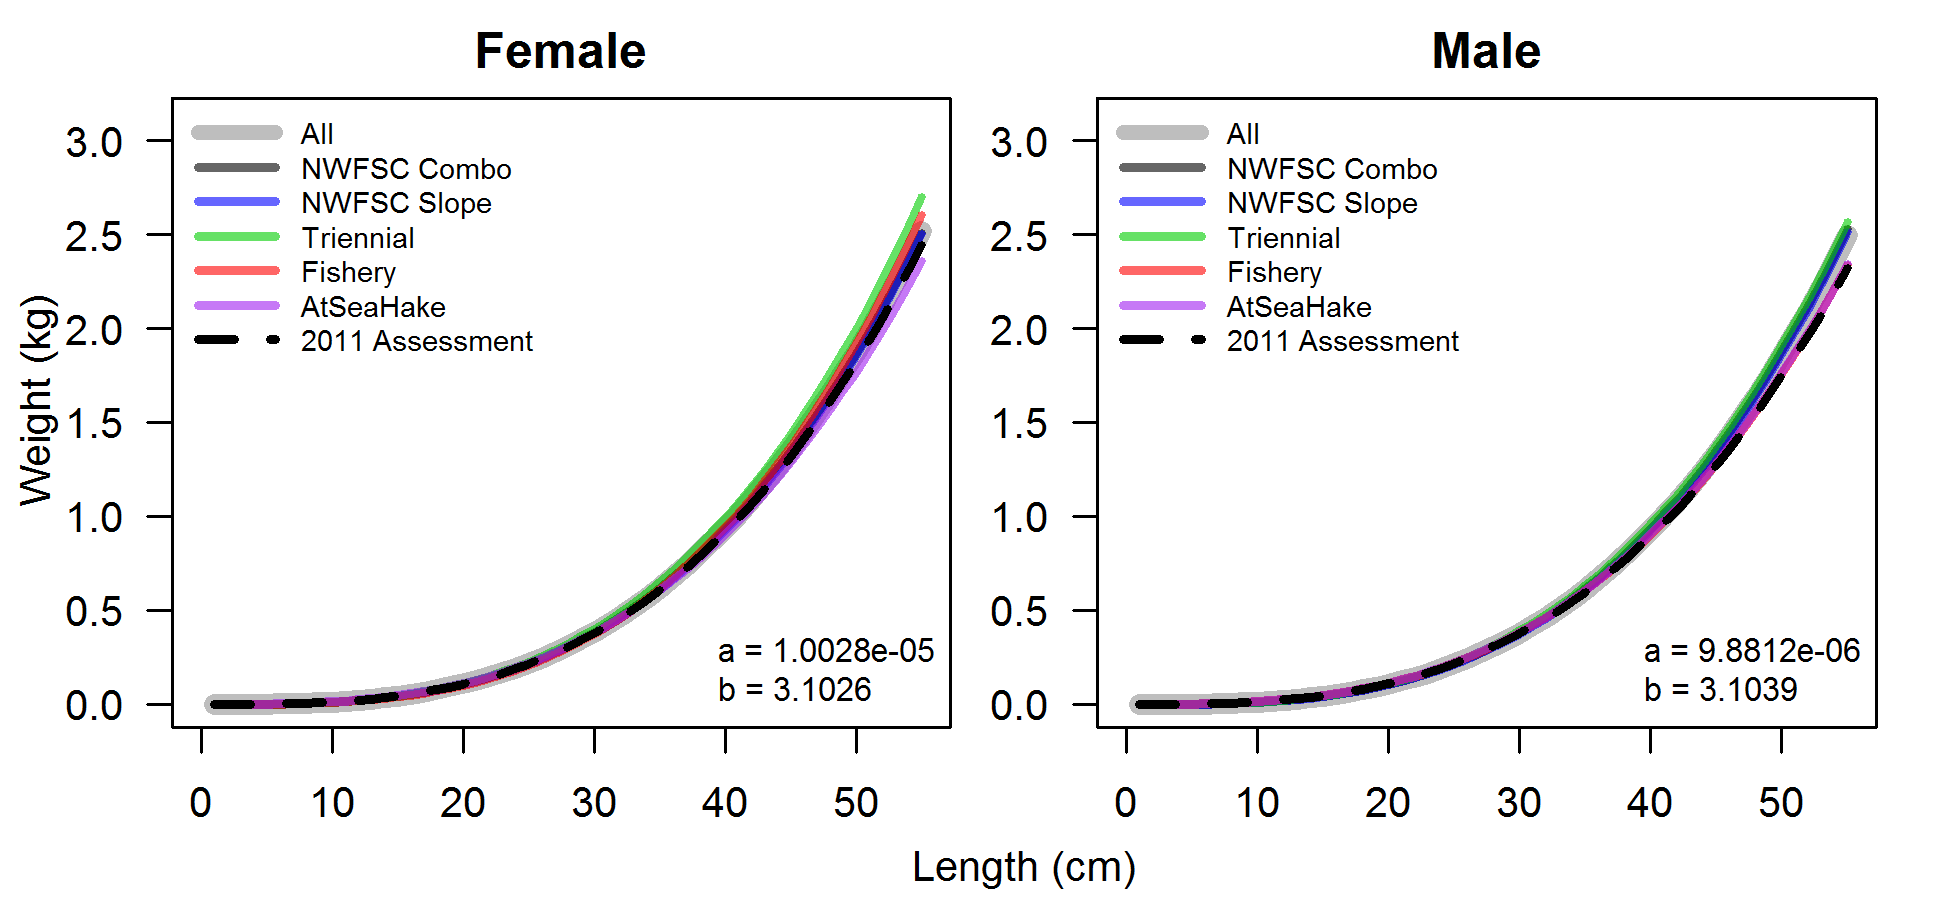
\includegraphics{Figures/weightAtLengthPred.png}
\caption{Estimated weight-at-length for female and male petrale sole.
\label{fig:wt_length}}
\end{figure}

\FloatBarrier

\begin{figure}
\centering
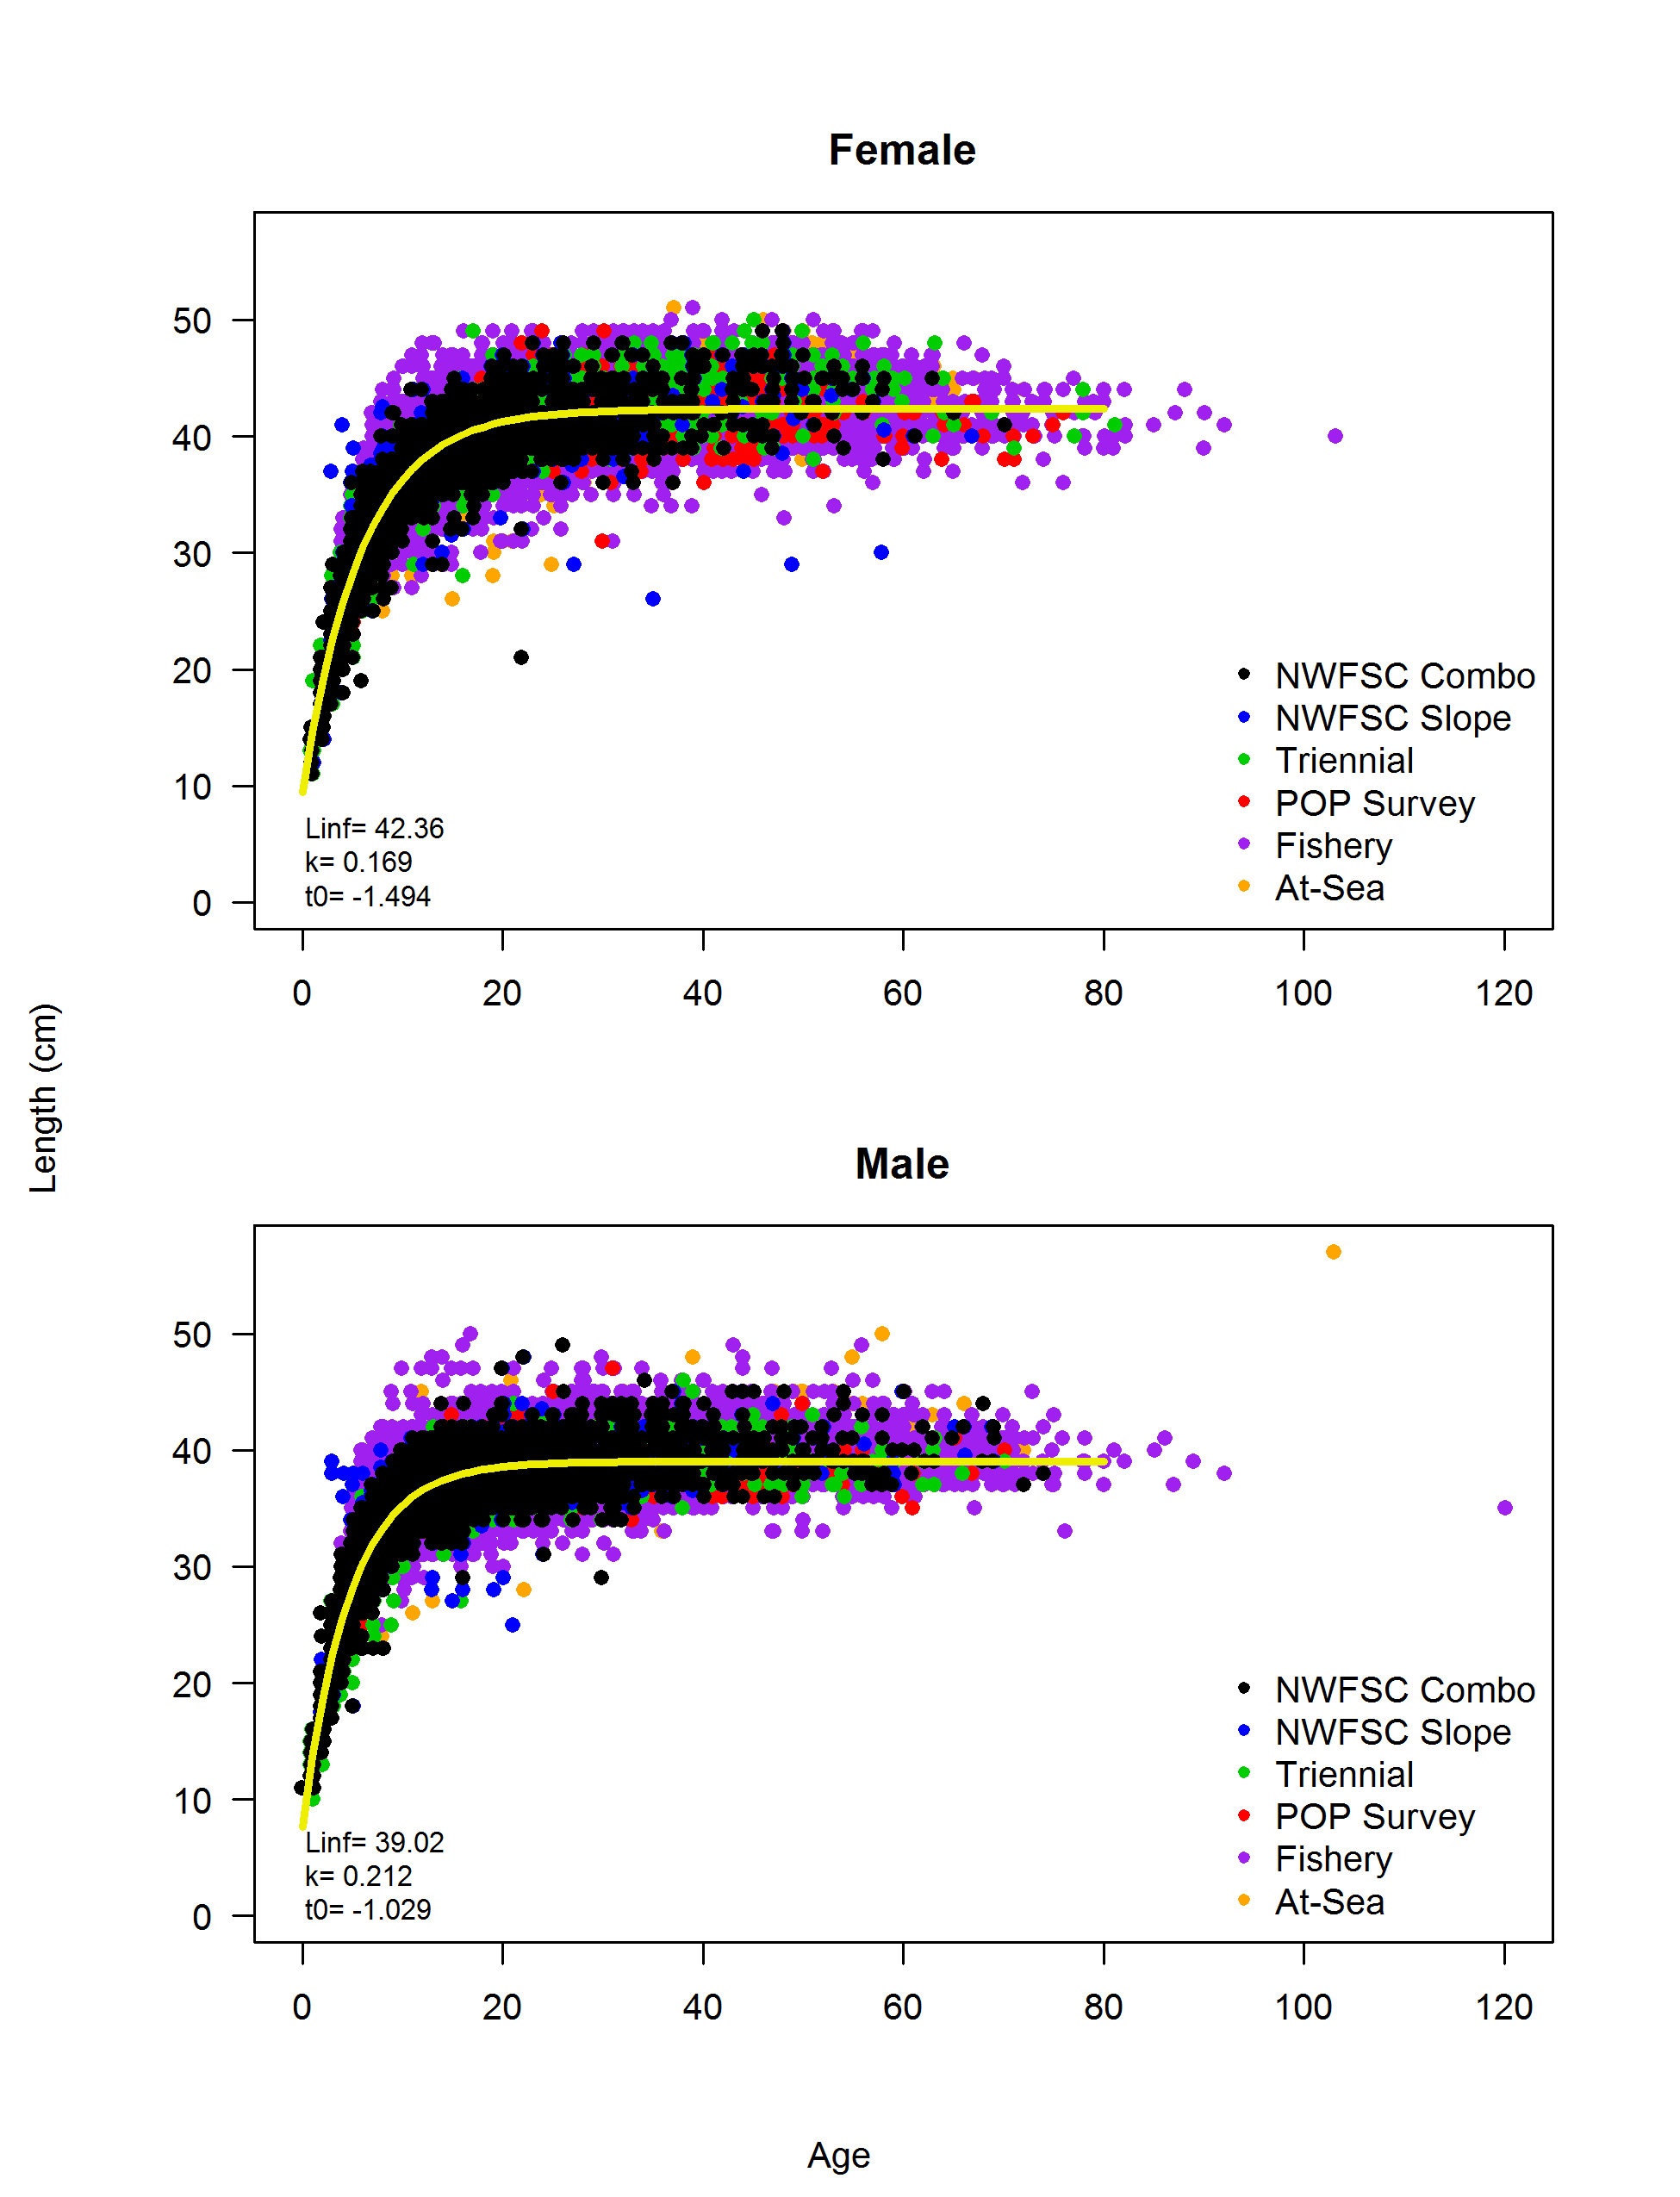
\includegraphics{Figures/LengthAgeAll.png}
\caption{Length-at-age across data sources for female and male petrale
sole. \label{fig:length_age}}
\end{figure}

\FloatBarrier

\begin{figure}
\centering
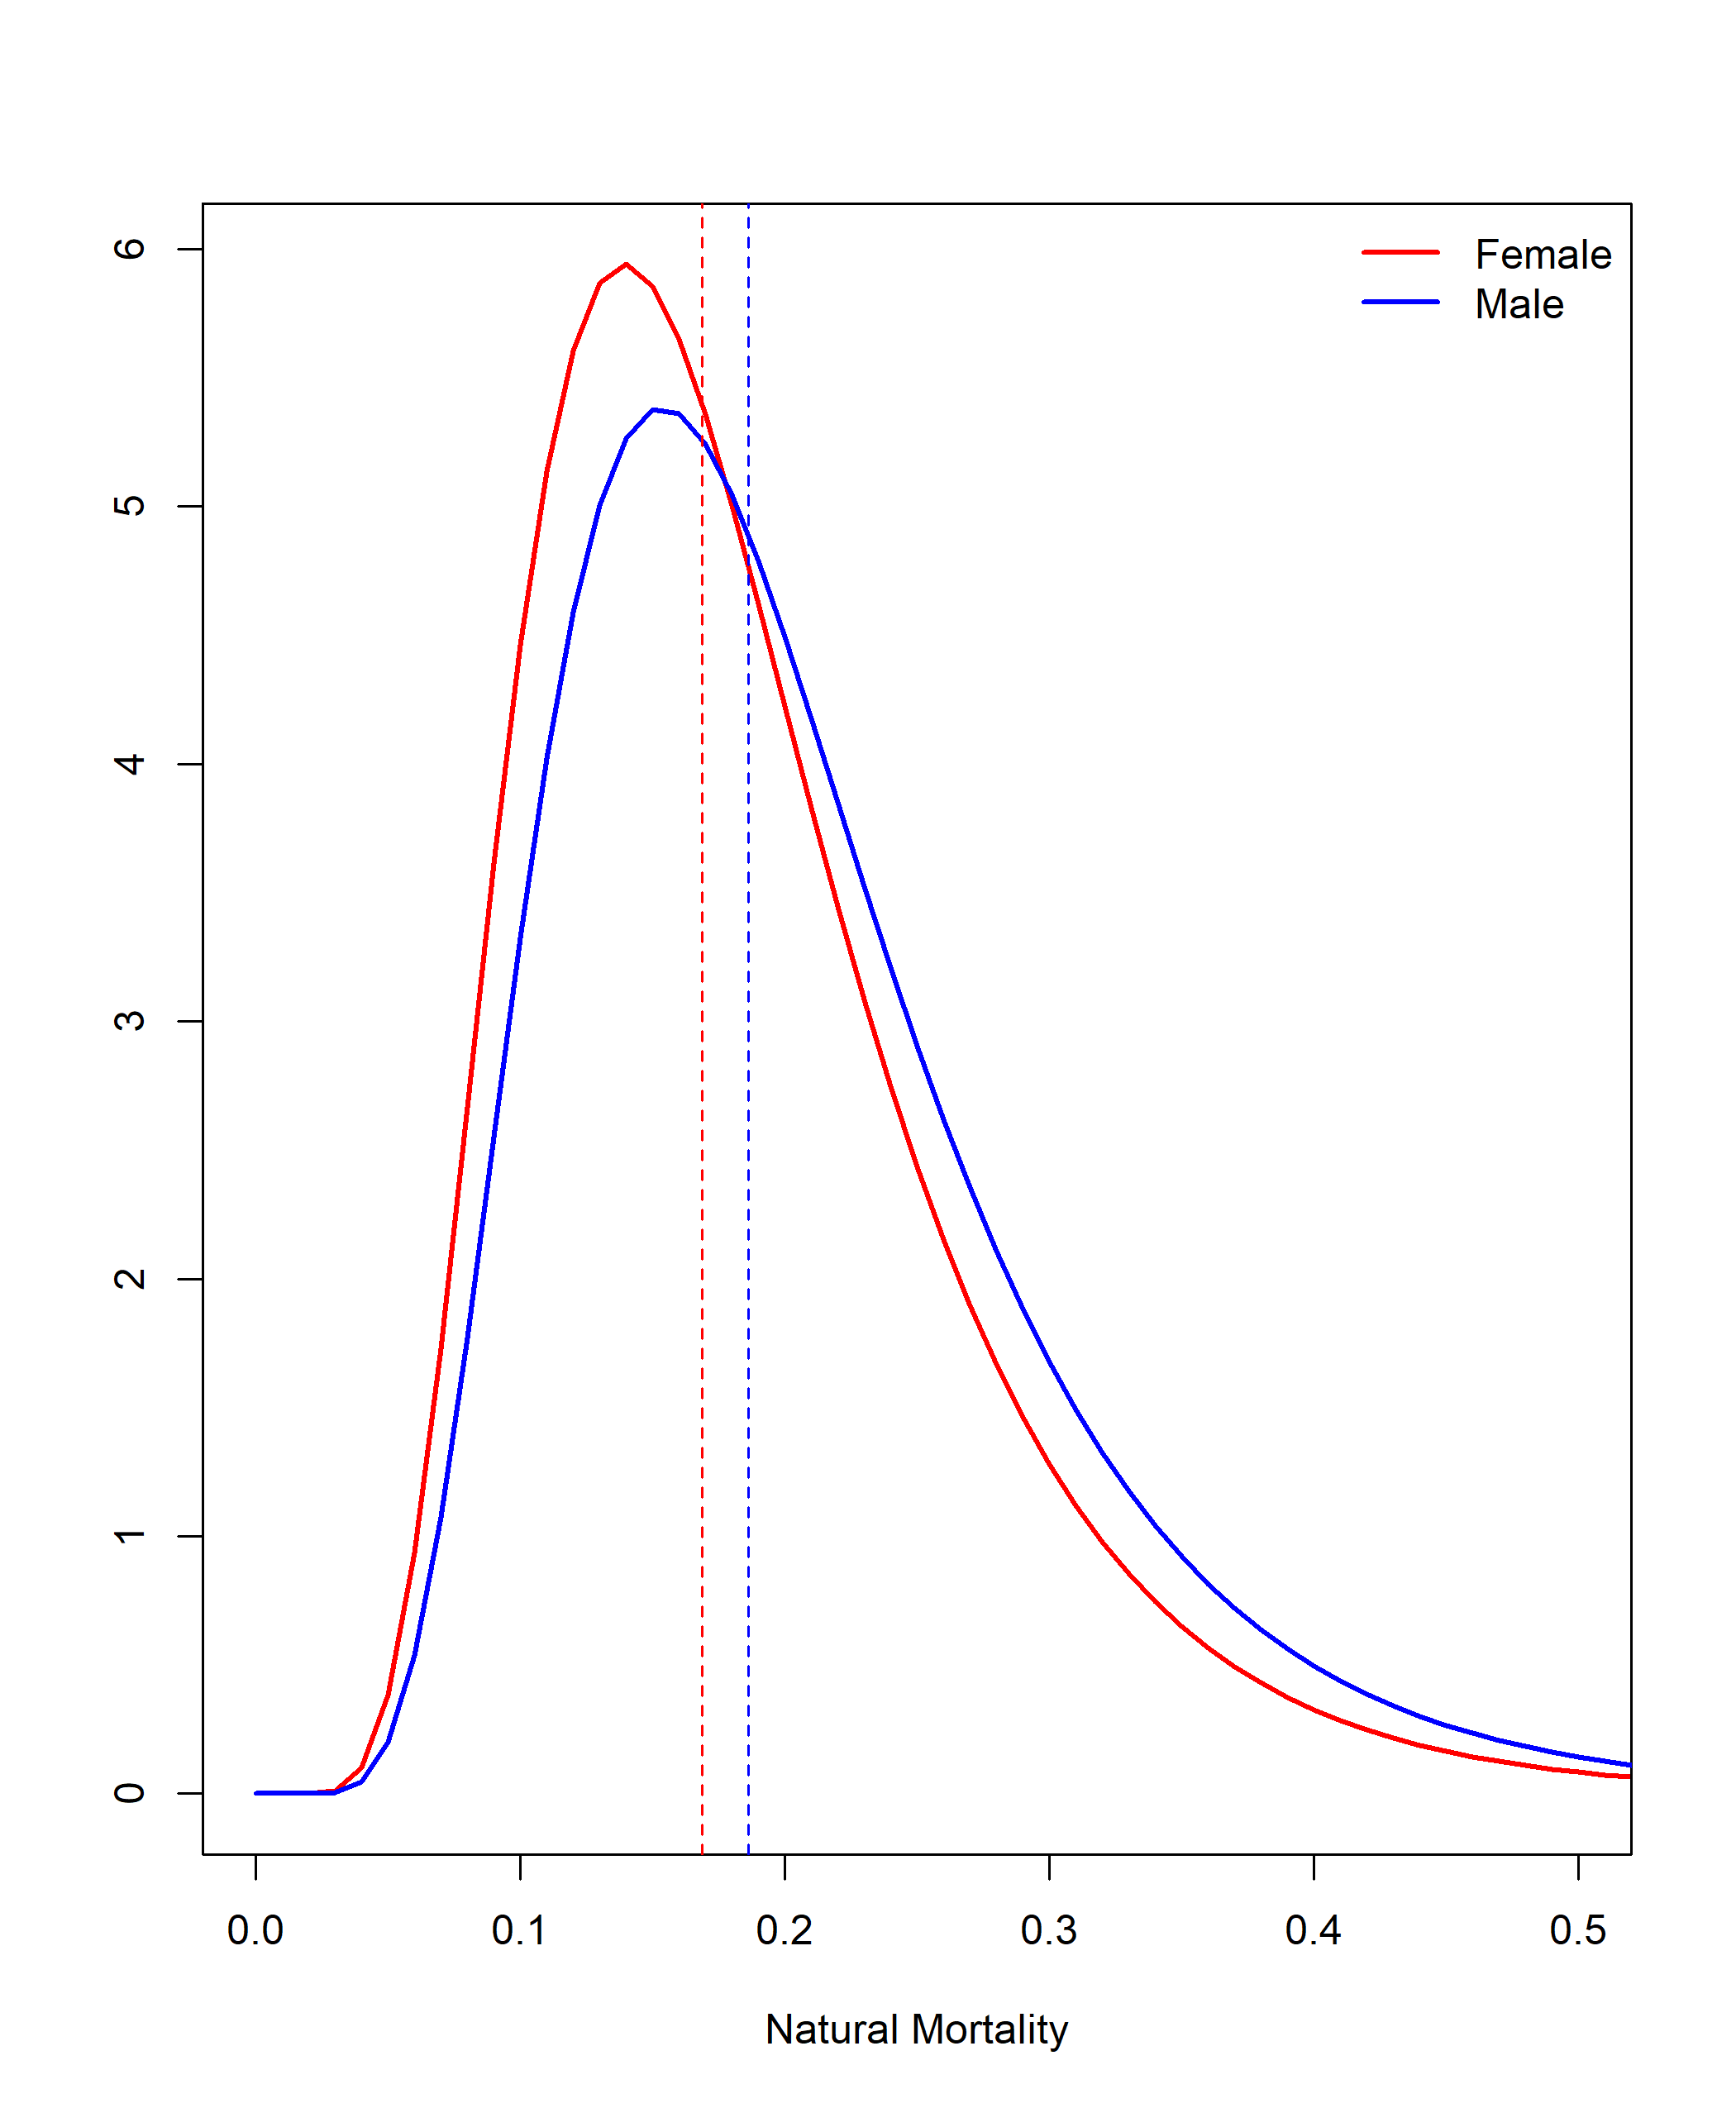
\includegraphics{Figures/M_prior.png}
\caption{Prior distribution for natural mortality for female and male
petrale sole. \label{fig:m_prior}}
\end{figure}

\FloatBarrier

\begin{figure}
\centering
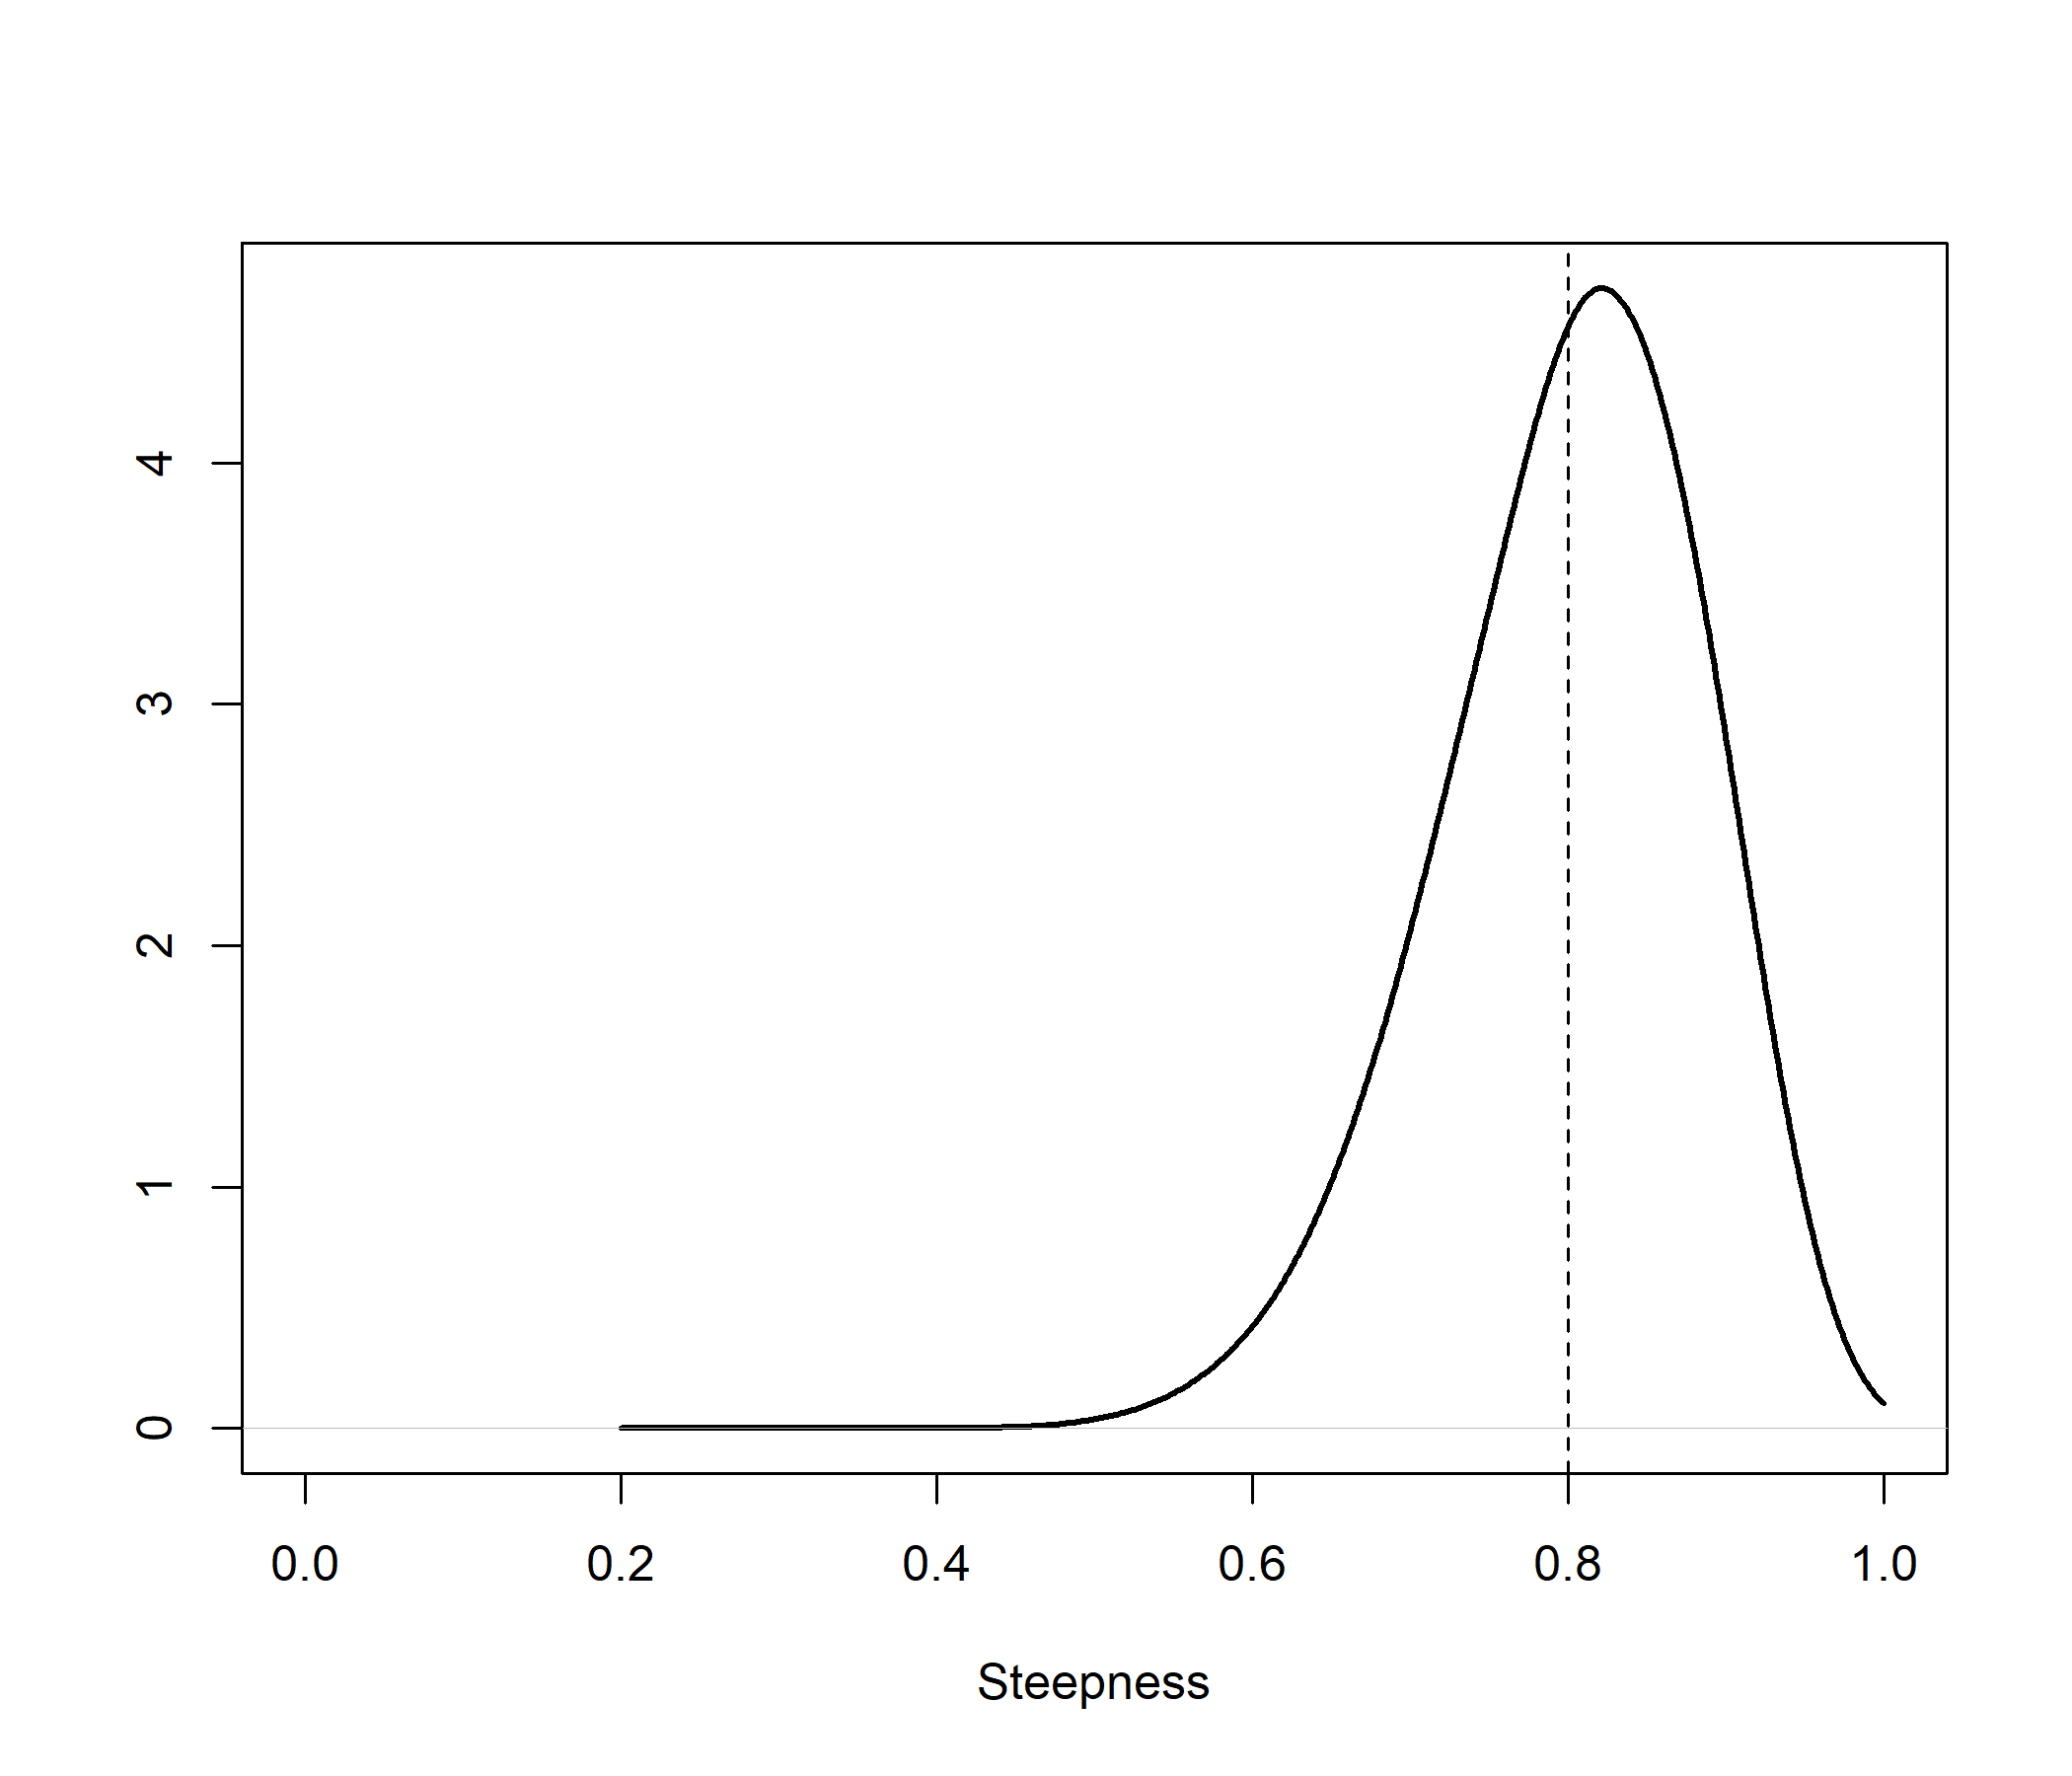
\includegraphics{Figures/h_prior.png}
\caption{Prior distribution for steepness petrale sole.
\label{fig:h_prior}}
\end{figure}

\FloatBarrier

\begin{figure}
\centering
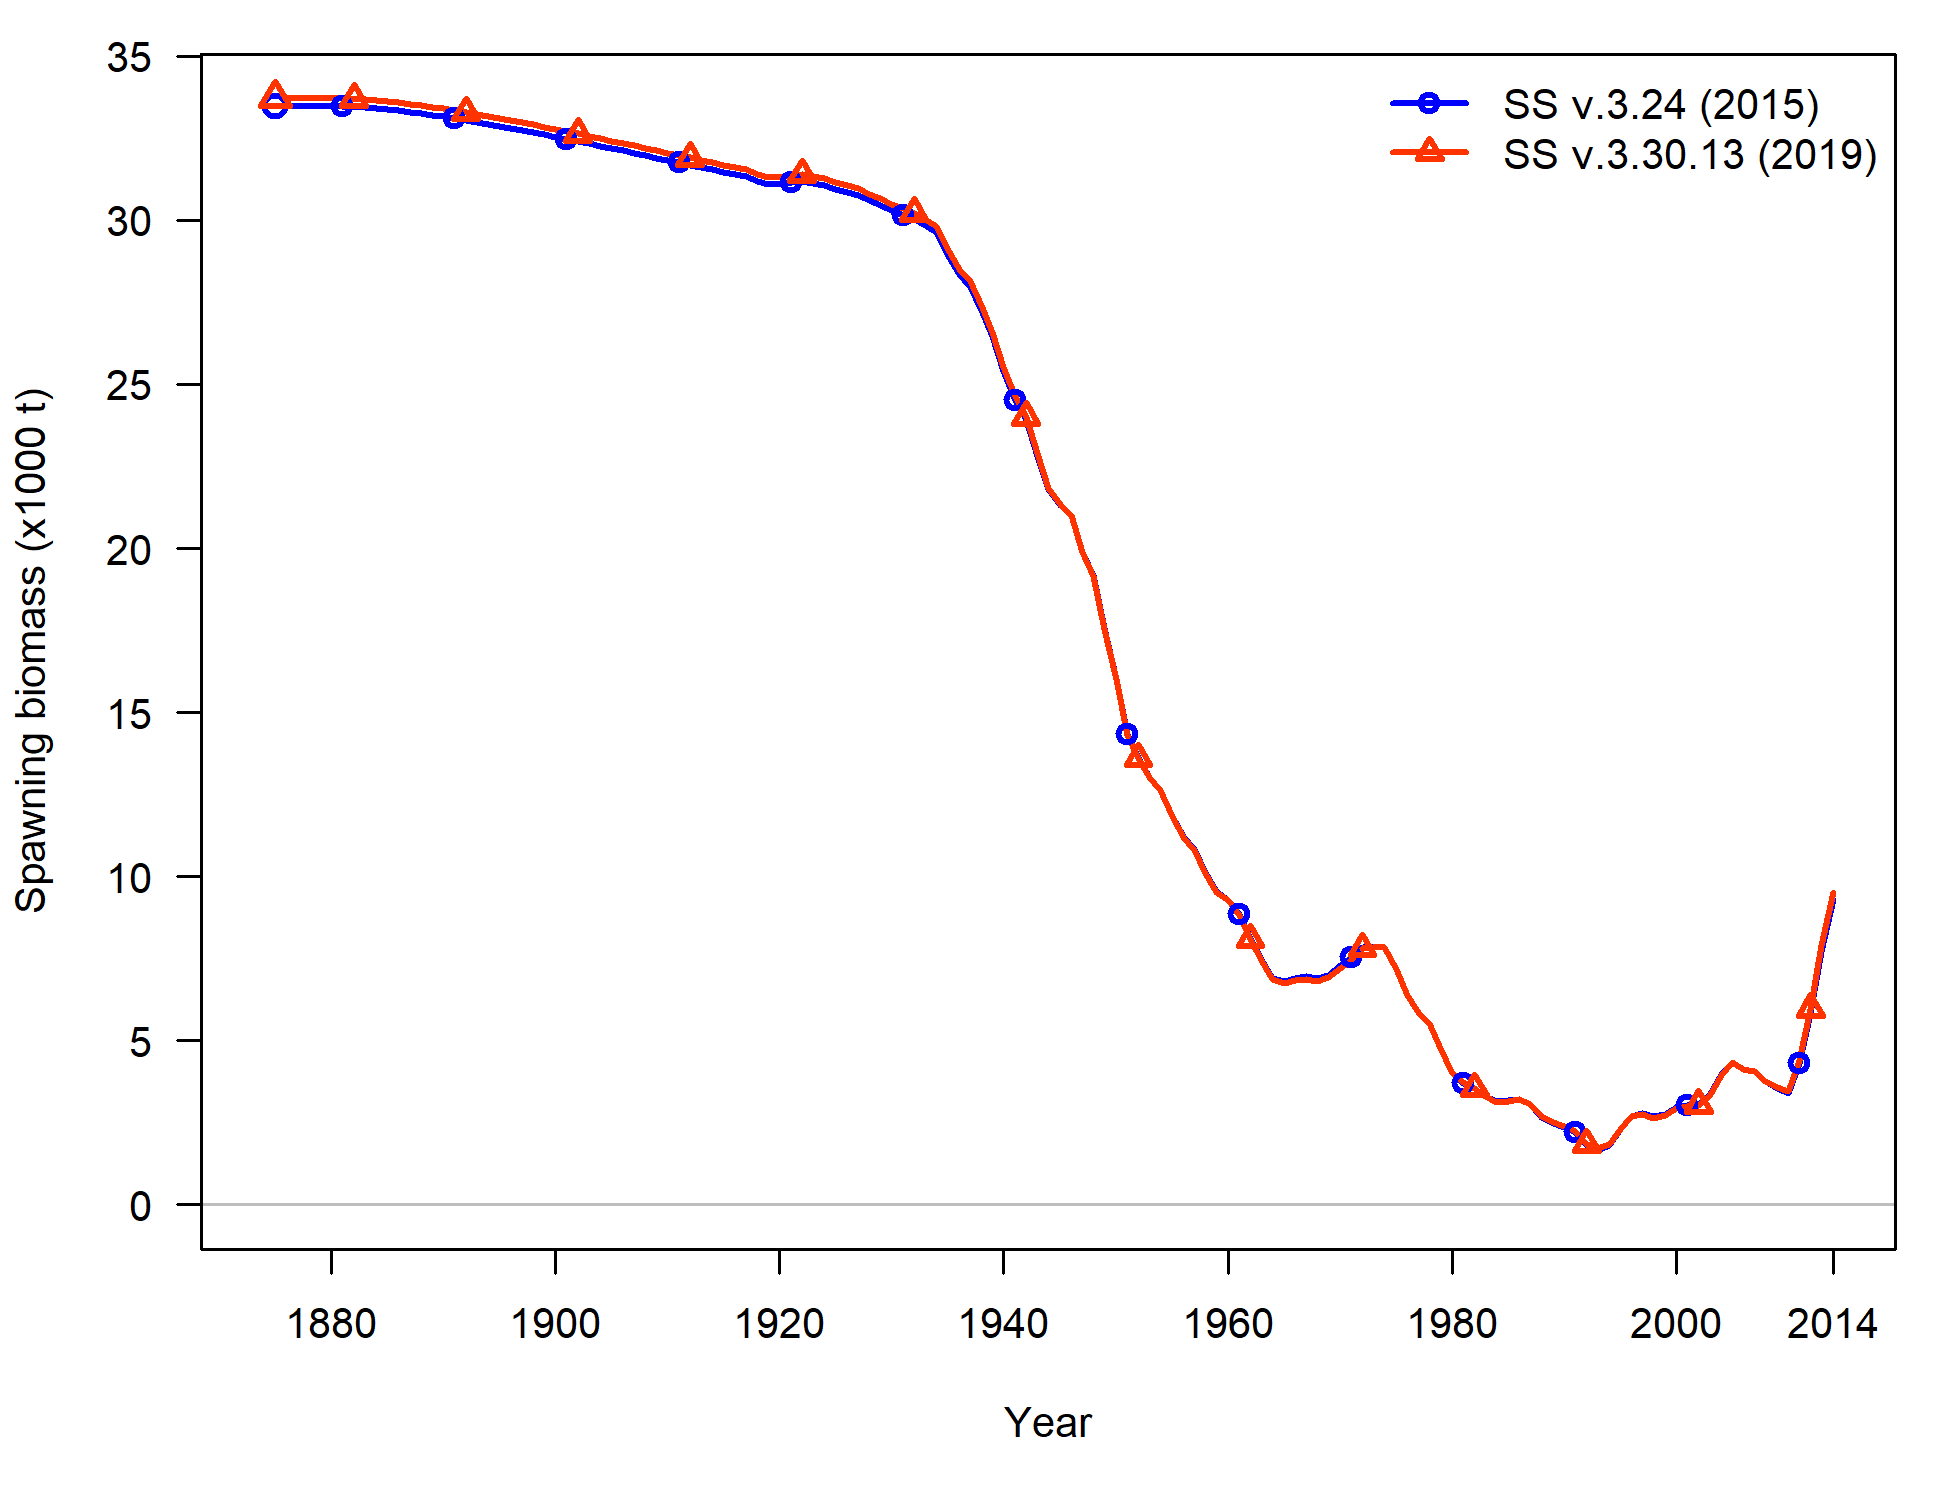
\includegraphics{Figures/compare1_spawnbio.png}
\caption{Comparison of model bridging estimates from Stock Synthesis
version 3.30.13 and 3.24U for petrale sole for the 2015 assessment.
\label{fig:bridge}}
\end{figure}

\FloatBarrier 

\begin{figure}
\centering
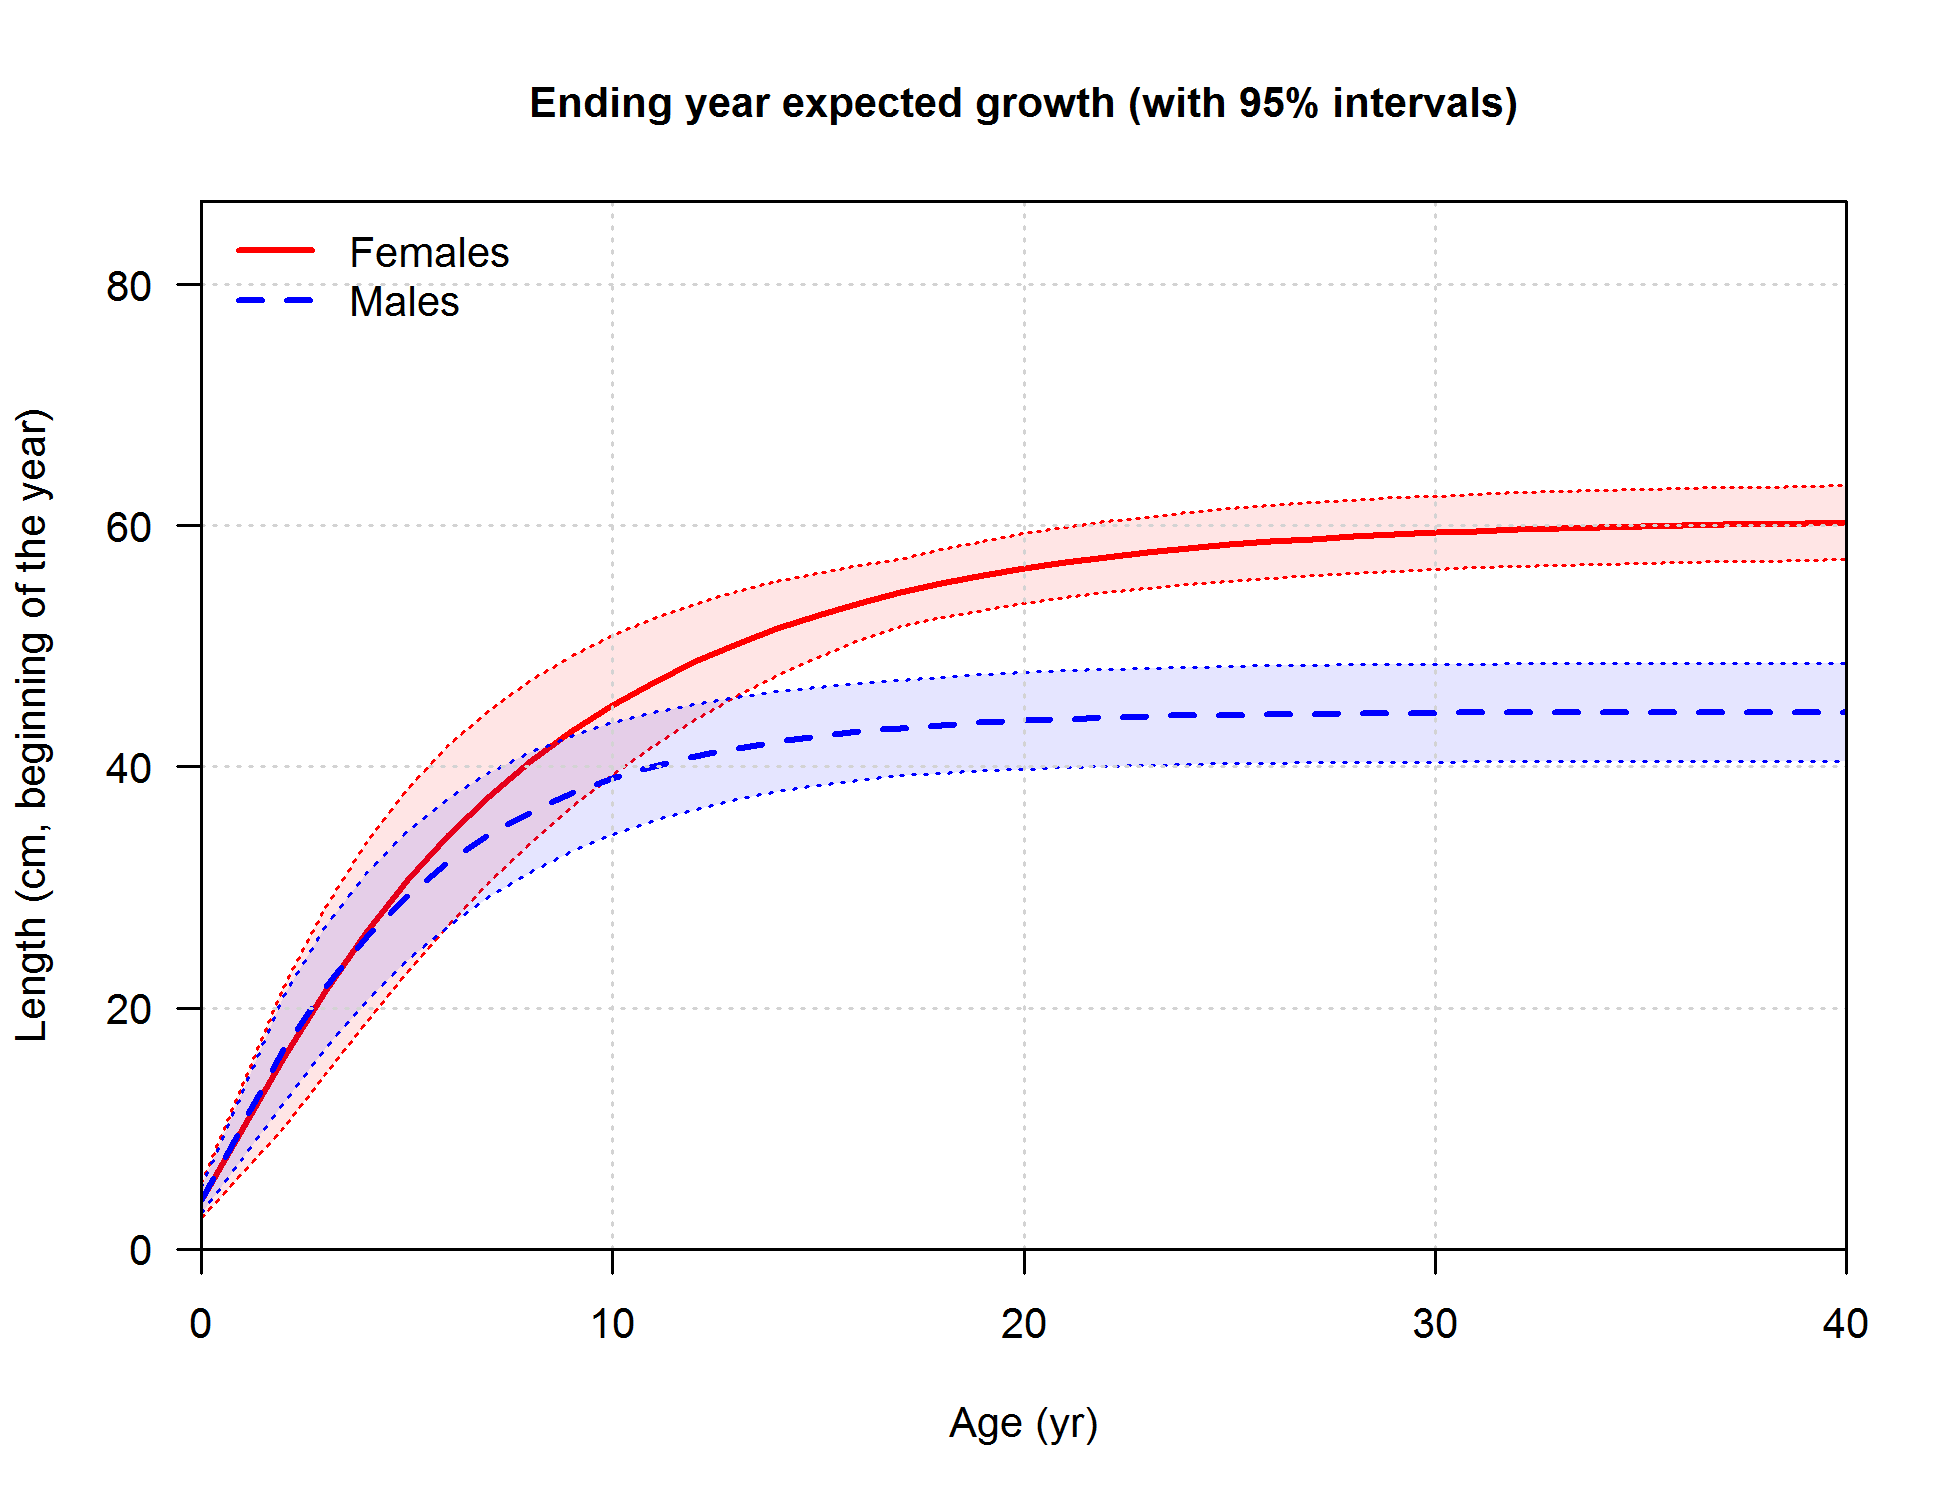
\includegraphics{r4ss/plots_mod1/bio1_sizeatage.png}
\caption{Estimated length-at-age for male and female for petrale sole
with estimated CV. \label{fig:sizeatage}}
\end{figure}

\FloatBarrier 

\begin{figure}
\centering
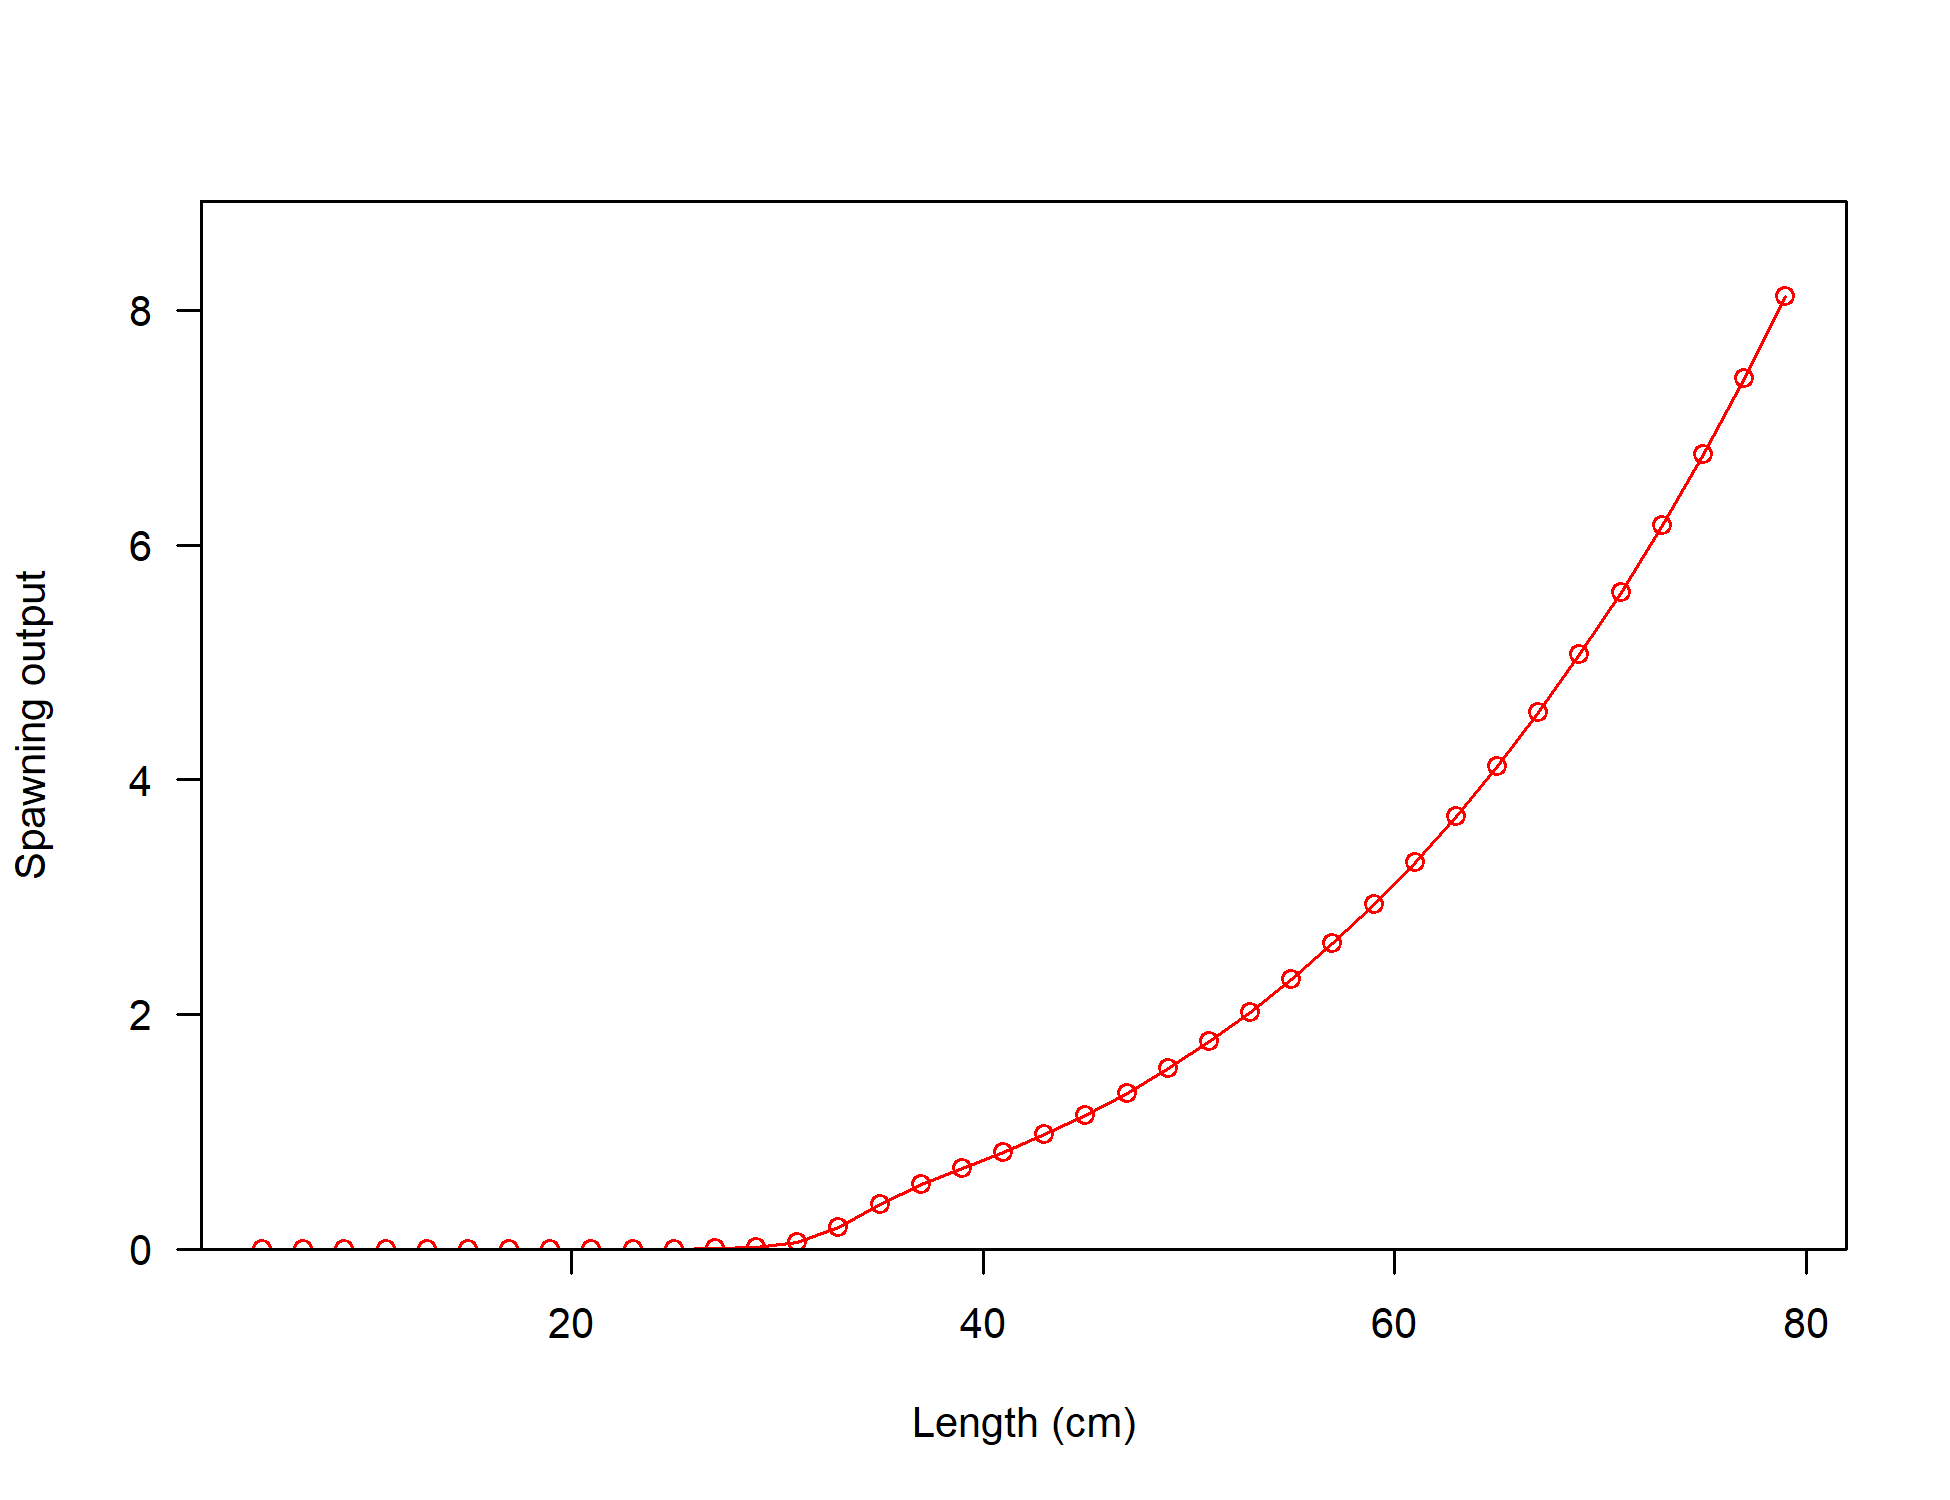
\includegraphics{r4ss/plots_mod1/bio10_spawningoutput_len.png}
\caption{Estimated spawning output-at-length for female petrale sole.
\label{fig:spawnoutlen}}
\end{figure}

\FloatBarrier 

\begin{figure}
\centering
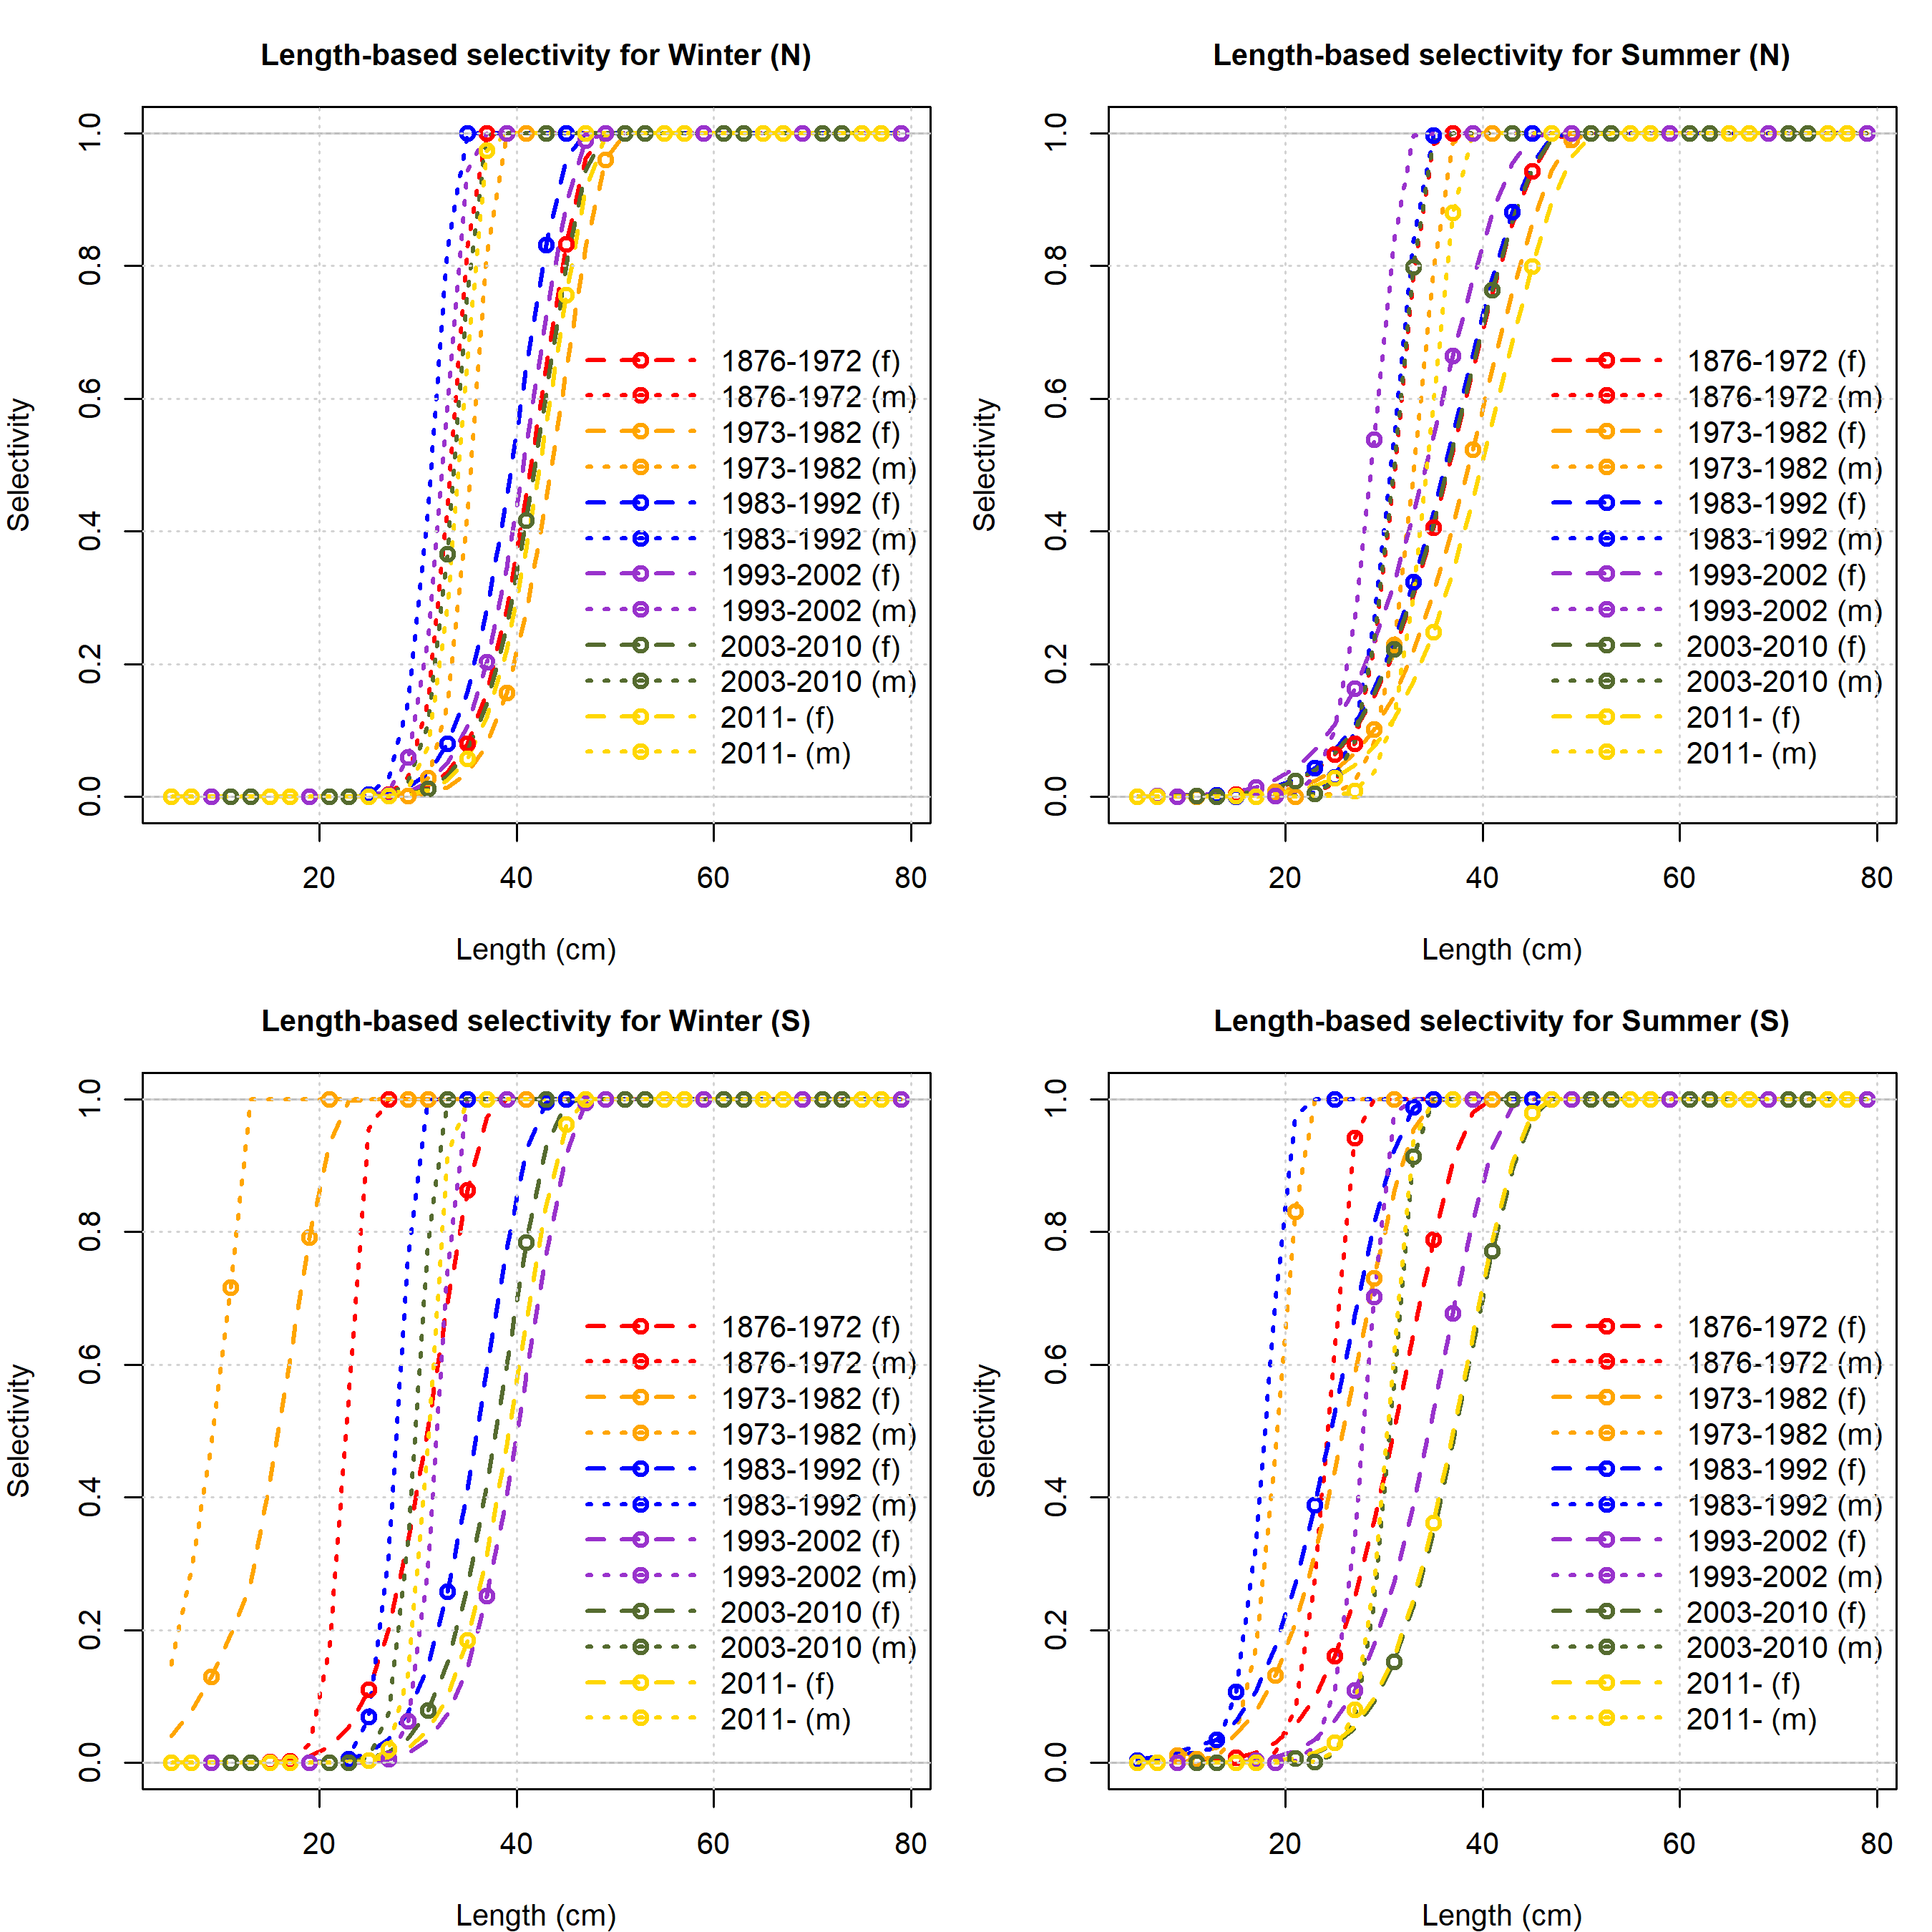
\includegraphics{Figures/Petrale_fishery_selectivity.png}
\caption{Estimated selectivity for each commerical fleet over the
assessment period for female and male petrale sole.
\label{fig:fish_selex}}
\end{figure}

\FloatBarrier

\begin{figure}
\centering
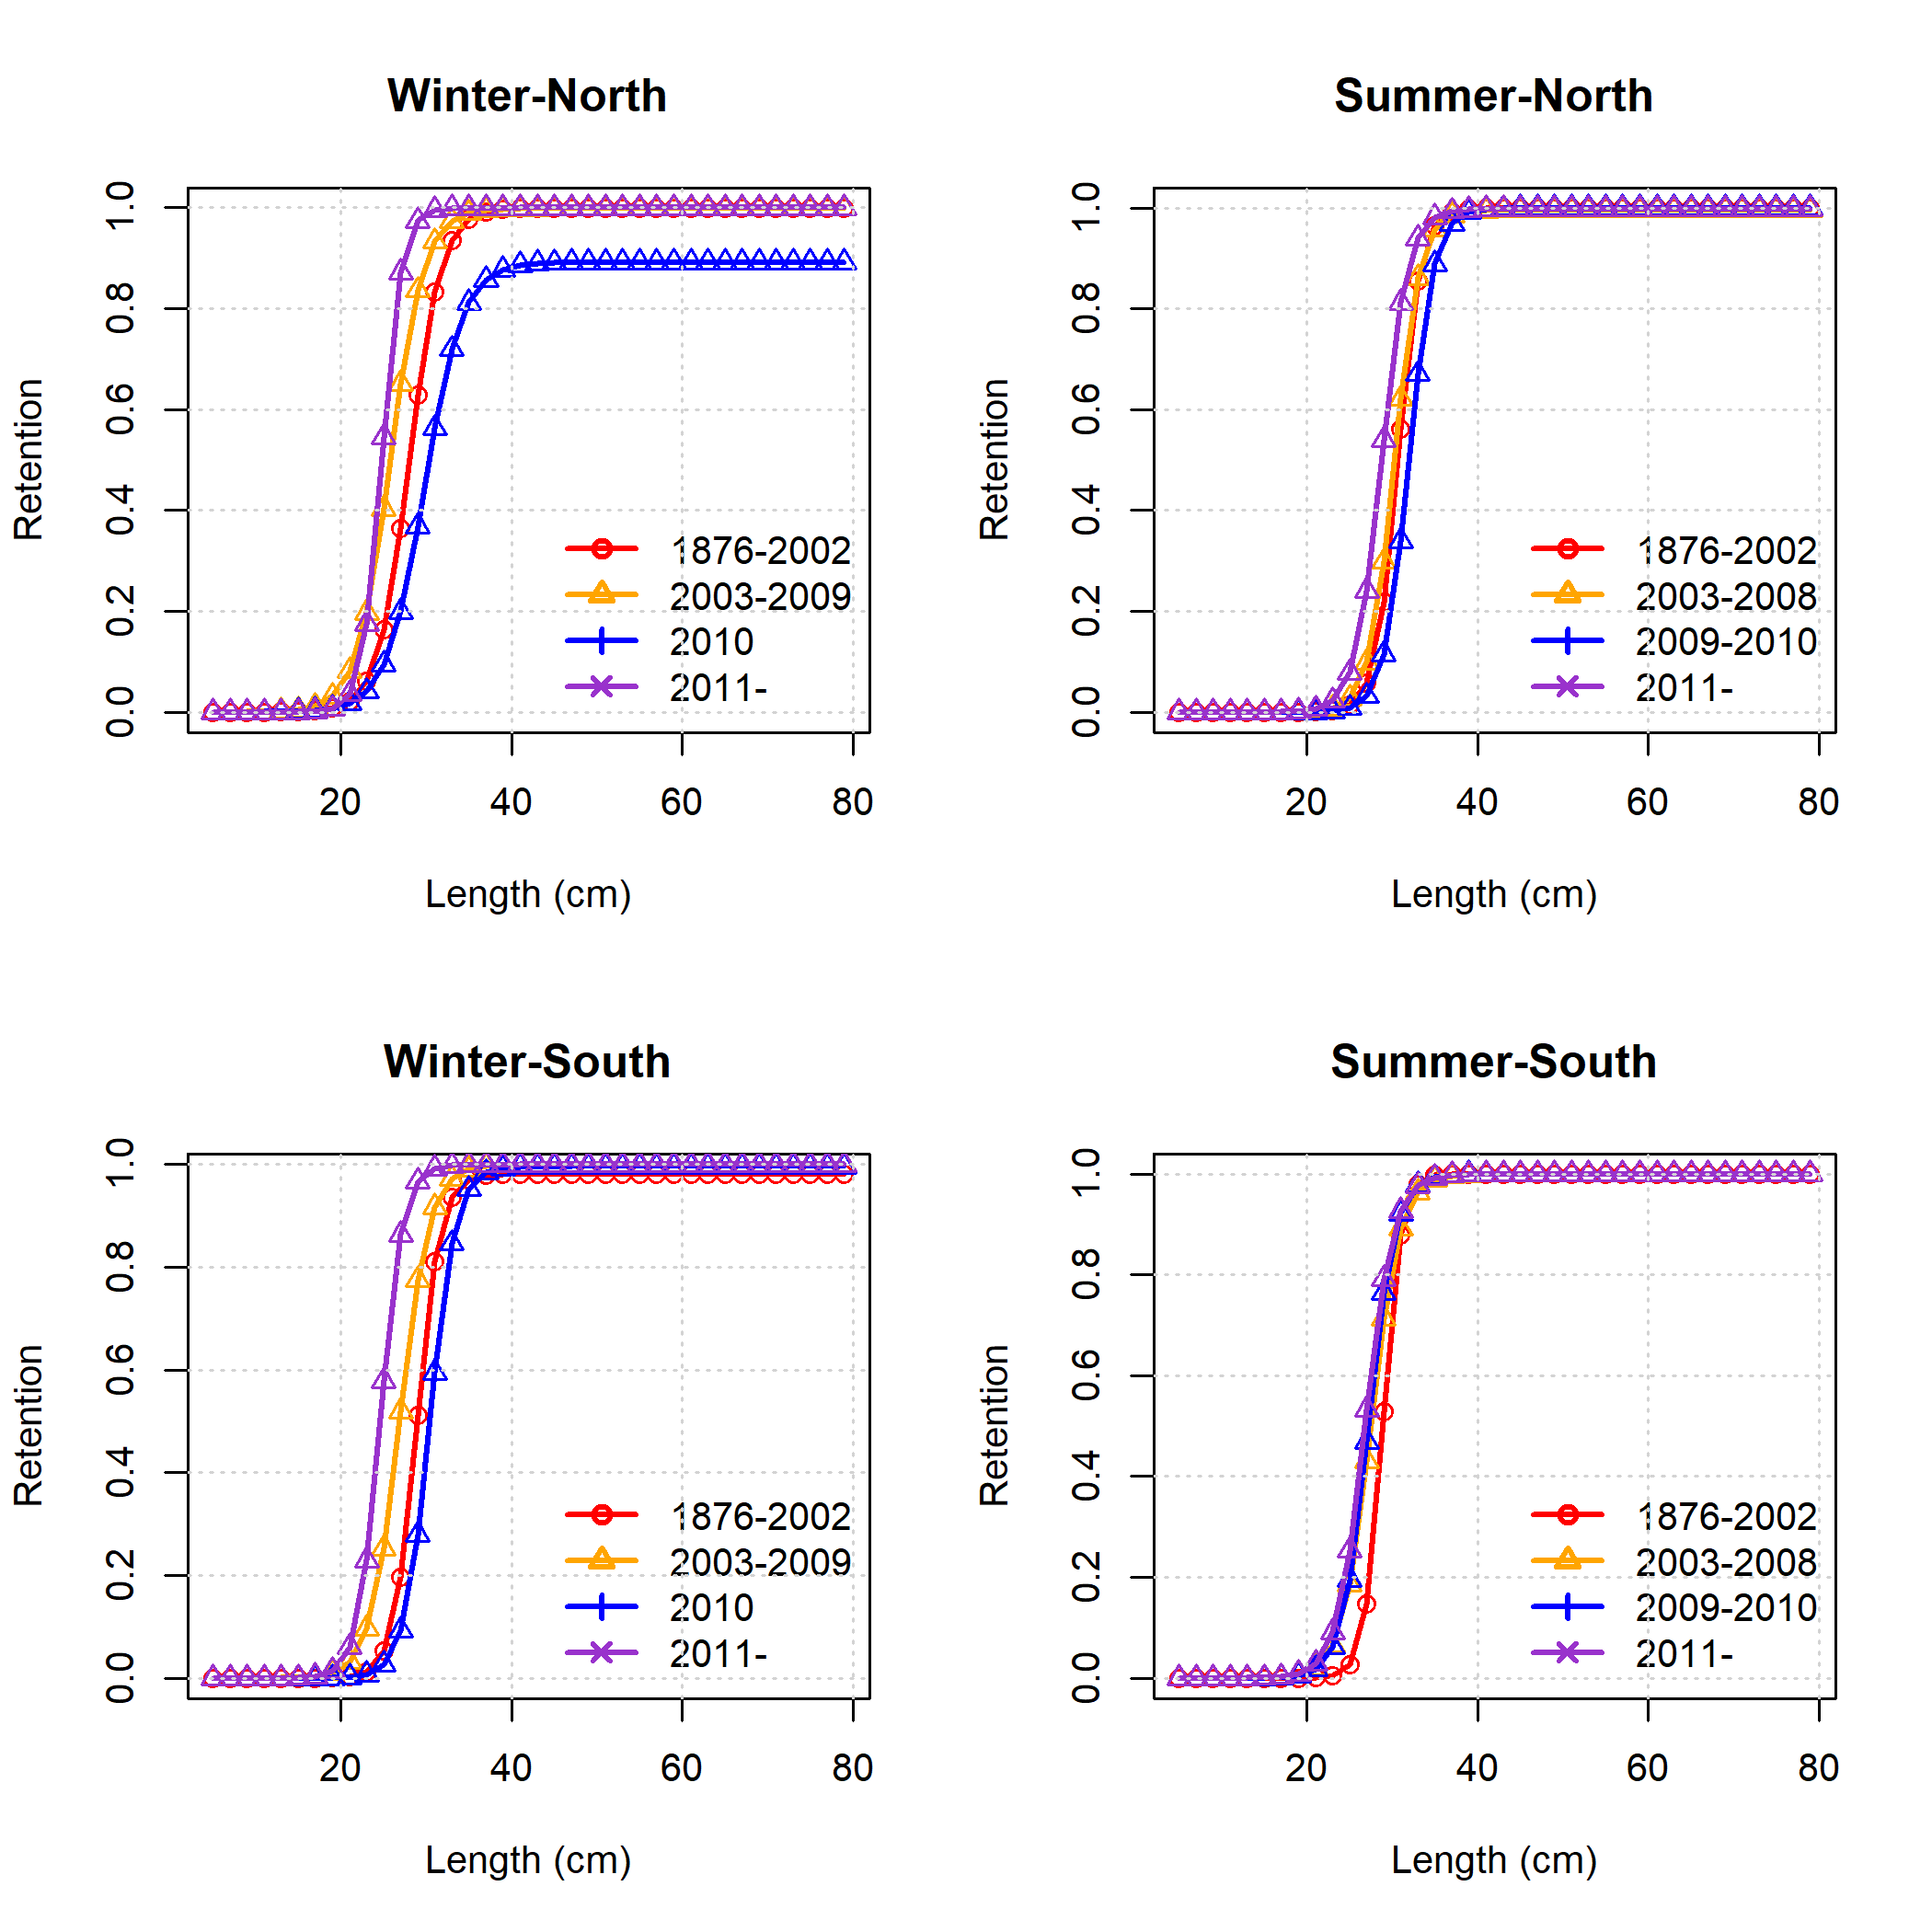
\includegraphics{Figures/Petrale_retention.png}
\caption{Estimated retention for each commerical fleet over the
assessment period for petrale sole. Retention was not estimated to be
sex-specific. \label{fig:fish_reten}}
\end{figure}

\FloatBarrier

\begin{figure}
\centering
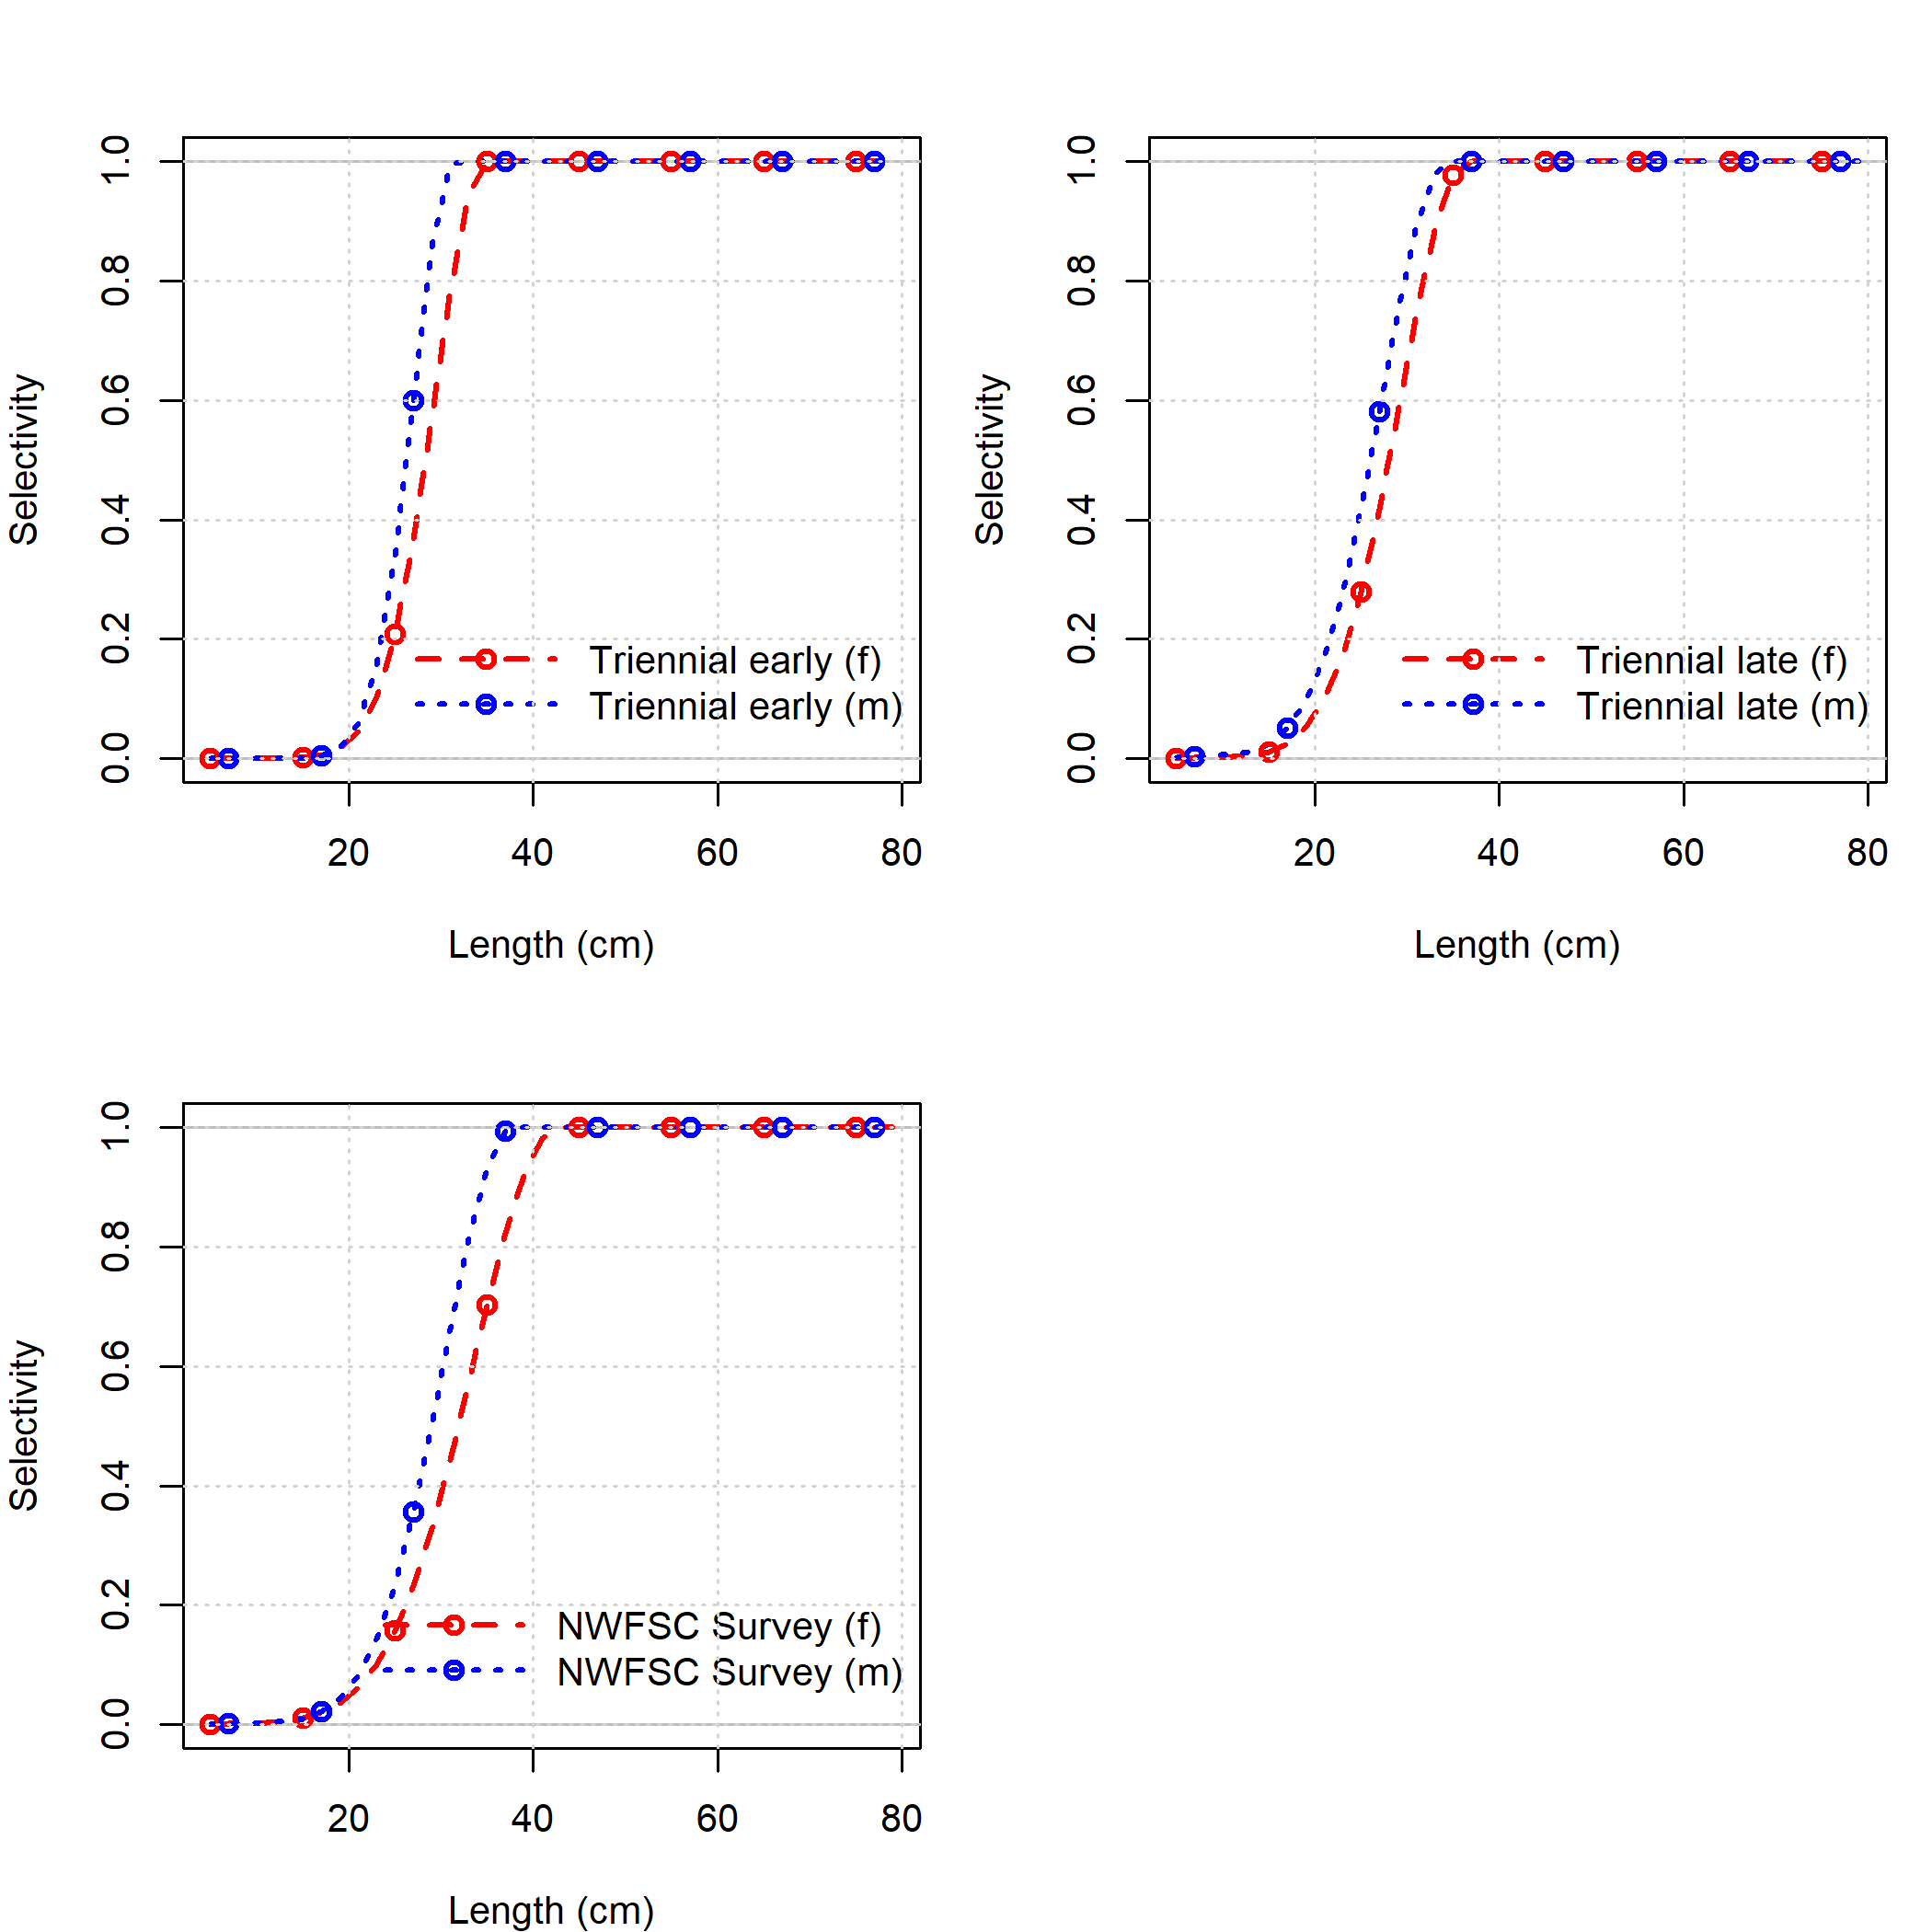
\includegraphics{Figures/Petrale_survey_selectivity.png}
\caption{Estimated selectivity for each survey over the assessment
period for female and male petrale sole. \label{fig:survey_selex}}
\end{figure}

\FloatBarrier

\begin{figure}
\centering
\includegraphics{r4ss/plots_mod1/ts11_Age-0_recruits_(1000s)_with_95_asymptotic_intervals.png}
\caption{Estimated time-series of recruitment for petrale sole.
\label{fig:recruits}}
\end{figure}

\FloatBarrier

\begin{figure}
\centering
\includegraphics{r4ss/plots_mod1/recdevs2_withbars.png}
\caption{Estimated time-series of recruitment deviations for petrale
sole. \label{fig:recdevs}}
\end{figure}

\FloatBarrier

\begin{figure}
\centering
\includegraphics{r4ss/plots_mod1/recdevs2_withbars.png}
\caption{Estimated recruitment deviations. \label{fig:rec_devs}}
\end{figure}

\FloatBarrier

\begin{figure}
\centering
\includegraphics{r4ss/plots_mod1/recruit_fit_bias_adjust.png}
\caption{Recruitment bias adjustment in the model.
\label{fig:bias_adjust}}
\end{figure}

\FloatBarrier

\begin{figure}
\centering
\includegraphics{r4ss/plots_mod1/index2_cpuefit_Winter (N).png}
\caption{Fit to the Winter North catch-per-unit-effort time series for
petrale sole. \label{fig:fit_wn_cpue}}
\end{figure}

\FloatBarrier

\begin{figure}
\centering
\includegraphics{r4ss/plots_mod1/index7_timevaryingQ_Winter (N).png}
\caption{Catchability to the Winter North catch-per-unit-effort time
series. \label{fig:q_north}}
\end{figure}

\FloatBarrier

\begin{figure}
\centering
\includegraphics{r4ss/plots_mod1/index2_cpuefit_Winter (S).png}
\caption{Fit to the Winter South catch-per-unit-effort time series for
petrale sole. \label{fig:fit_ws_cpue}}
\end{figure}

\FloatBarrier

\begin{figure}
\centering
\includegraphics{r4ss/plots_mod1/index7_timevaryingQ_Winter (S).png}
\caption{Catchability to the Winter South catch-per-unit-effort time
series. \label{fig:q_south}}
\end{figure}

\FloatBarrier

\begin{figure}
\centering
\includegraphics{r4ss/plots_mod1/index2_cpuefit_Triennial - Early.png}
\caption{Fit to the Triennial Survey Early time series for petrale sole.
\label{fig:fit_tri_early}}
\end{figure}

\FloatBarrier 

\begin{figure}
\centering
\includegraphics{r4ss/plots_mod1/index2_cpuefit_Triennial - Late.png}
\caption{Fit to the Triennial Survey Late time series for petrale sole.
\label{fig:fit_tri_late}}
\end{figure}

\FloatBarrier 

\begin{figure}
\centering
\includegraphics{r4ss/plots_mod1/index2_cpuefit_NWFSC West Coast Groundfish Bottom Trawl Survey.png}
\caption{Fit to the NWFSC West Coast Groundfish Bottom Trawl Survey time
series for petrale sole. \label{fig:fit_nwfsc_survey}}
\end{figure}

\FloatBarrier

\begin{figure}
\centering
\includegraphics{r4ss/plots_mod1/discard_fitWinter (N).png}
\caption{Fit to the discard rates for the Winter North fleet for petrale
sole. \label{fig:fit_wn_discard}}
\end{figure}

\FloatBarrier

\begin{figure}
\centering
\includegraphics{r4ss/plots_mod1/discard_fitSummer (N).png}
\caption{Fit to the discard rates for the Summer North fleet for petrale
sole. \label{fig:fit_sn_discard}}
\end{figure}

\FloatBarrier

\begin{figure}
\centering
\includegraphics{r4ss/plots_mod1/discard_fitWinter (S).png}
\caption{Fit to the discard rates for the Winter South fleet for petrale
sole. \label{fig:fit_ws_discard}}
\end{figure}

\FloatBarrier

\begin{figure}
\centering
\includegraphics{r4ss/plots_mod1/discard_fitSummer (S).png}
\caption{Fit to the discard rates for the Summer South fleet for petrale
sole. \label{fig:fit_ss_discard}}
\end{figure}

\FloatBarrier

\begin{figure}
\centering
\includegraphics{r4ss/plots_mod1/catch8 discard fraction.png}
\caption{Discard rates by fleet for petrale sole. \label{fig:Discard}}
\end{figure}

\FloatBarrier

\begin{figure}
\centering
\includegraphics{r4ss/plots_mod1/bodywt_fit_fltWinter (N).png}
\caption{Fit to the Northern winter fishery mean body weights of
discarded fish for petrale sole. \label{fig:nw_bodywt_fit}}
\end{figure}

\FloatBarrier

\begin{figure}
\centering
\includegraphics{r4ss/plots_mod1/bodywt_fit_fltSummer (N).png}
\caption{Fit to the Northern summer fishery mean body weights of
discarded fish for petrale sole. \label{fig:ns_bodywt_fit}}
\end{figure}

\FloatBarrier

\begin{figure}
\centering
\includegraphics{r4ss/plots_mod1/bodywt_fit_fltWinter (S).png}
\caption{Fit to the Southern winter fishery mean body weights of
discarded fish for petrale sole. \label{fig:sw_bodywt_fit}}
\end{figure}

\FloatBarrier

\begin{figure}
\centering
\includegraphics{r4ss/plots_mod1/bodywt_fit_fltSummer (S).png}
\caption{Fit to the Southern summer fishery mean body weights of
discarded fish for petrale sole. \label{fig:ss_bodywt_fit}}
\end{figure}

\FloatBarrier

\begin{figure}
\centering
\includegraphics{r4ss/plots_mod1/comp_lenfit__aggregated_across_time.png}
\caption{Length compositions aggregated across time by fleet. Labels
`retained' and `discard' indicate retained or discarded samples for each
fleet. Panels without this designation represent the whole catch.
\label{fig:length_agg}}
\end{figure}

\FloatBarrier

\begin{figure}
\centering
\includegraphics{r4ss/plots_mod1/comp_lenfit_residsflt1mkt1.png}
\caption{Pearson residuals, discard, Winter (N) (max=7.19)\\
Closed bubbles are positive residuals (observed \textgreater{} expected)
and open bubbles are negative residuals (observed \textless{} expected).
\label{fig:discard_wn_len_pearson}}
\end{figure}

\begin{figure}
\centering
\includegraphics{r4ss/plots_mod1/comp_lenfit_residsflt2mkt1.png}
\caption{Pearson residuals, discard, Summer (N) (max=6.6)\\
Closed bubbles are positive residuals (observed \textgreater{} expected)
and open bubbles are negative residuals (observed \textless{} expected).
\label{fig:discard_sn_len_pearson}}
\end{figure}

\begin{figure}
\centering
\includegraphics{r4ss/plots_mod1/comp_lenfit_residsflt3mkt1.png}
\caption{Pearson residuals, discard, Winter (S) (max=3.81)\\
Closed bubbles are positive residuals (observed \textgreater{} expected)
and open bubbles are negative residuals (observed \textless{} expected).
\label{fig:discard_ws_len_pearson}}
\end{figure}

\begin{figure}
\centering
\includegraphics{r4ss/plots_mod1/comp_lenfit_residsflt4mkt1.png}
\caption{Pearson residuals, discard, Summer (S) (max=5.02)\\
Closed bubbles are positive residuals (observed \textgreater{} expected)
and open bubbles are negative residuals (observed \textless{} expected).
\label{fig:discard_ss_len_pearson}}
\end{figure}

\begin{figure}
\centering
\includegraphics{r4ss/plots_mod1/comp_lenfit_residsflt1mkt2_page4.png}
\caption{Pearson residuals, retained, Winter (N) (max=3.93) (plot 4 of
4)\\
Closed bubbles are positive residuals (observed \textgreater{} expected)
and open bubbles are negative residuals (observed \textless{} expected).
\label{fig:wn_len_pearson}}
\end{figure}

\begin{figure}
\centering
\includegraphics{r4ss/plots_mod1/comp_lenfit_residsflt2mkt2_page4.png}
\caption{Pearson residuals, retained, Summer (N) (max=5.15) (plot 4 of
4)\\
Closed bubbles are positive residuals (observed \textgreater{} expected)
and open bubbles are negative residuals (observed \textless{} expected).
\label{fig:sn_len_pearson}}
\end{figure}

\begin{figure}
\centering
\includegraphics{r4ss/plots_mod1/comp_lenfit_residsflt3mkt2_page3.png}
\caption{Pearson residuals, retained, Winter (S) (max=5.1) (plot 3 of
3)\\
Closed bubbles are positive residuals (observed \textgreater{} expected)
and open bubbles are negative residuals (observed \textless{} expected).
\label{fig:ws_len_pearson}}
\end{figure}

\begin{figure}
\centering
\includegraphics{r4ss/plots_mod1/comp_lenfit_residsflt4mkt2_page4.png}
\caption{Pearson residuals, retained, Summer (S) (max=5.63) (plot 4 of
4)\\
Closed bubbles are positive residuals (observed \textgreater{} expected)
and open bubbles are negative residuals (observed \textless{} expected).
\label{fig:ss_len_pearson}}
\end{figure}

\begin{figure}
\centering
\includegraphics{r4ss/plots_mod1/comp_lenfit_residsflt5mkt0.png}
\caption{Pearson residuals, whole catch, Triennial \_ Early (max=3.16)\\
Closed bubbles are positive residuals (observed \textgreater{} expected)
and open bubbles are negative residuals (observed \textless{} expected).
\label{fig:tri_early_len_pearson}}
\end{figure}

\begin{figure}
\centering
\includegraphics{r4ss/plots_mod1/comp_lenfit_residsflt6mkt0.png}
\caption{Pearson residuals, whole catch, Triennial \_ Late (max=3.54)\\
Closed bubbles are positive residuals (observed \textgreater{} expected)
and open bubbles are negative residuals (observed \textless{} expected).
\label{fig:tri_late_len_pearson}}
\end{figure}

\begin{figure}
\centering
\includegraphics{r4ss/plots_mod1/comp_lenfit_residsflt7mkt0.png}
\caption{Pearson residuals, whole catch, NWFSC West Coast Groundfish
Bottom Trawl Survey (max=5.11)\\
Closed bubbles are positive residuals (observed \textgreater{} expected)
and open bubbles are negative residuals (observed \textless{} expected).
\label{fig:nwfsc_combo_len_pearson}}
\end{figure}

\begin{figure}
\centering
\includegraphics{r4ss/plots_mod1/comp_lenfit_sampsize_flt1mkt2.png}
\caption{McAllister and Ianelli (harmonic mean) weighting for the Winter
North fishery length data. \label{fig:harm_mean_wn}}
\end{figure}

\FloatBarrier

\begin{figure}
\centering
\includegraphics{r4ss/plots_mod1/comp_lenfit_sampsize_flt2mkt2.png}
\caption{McAllister and Ianelli (harmonic mean) weighting for the Summer
North fishery length data. \label{fig:harm_mean_sn}}
\end{figure}

\FloatBarrier

\begin{figure}
\centering
\includegraphics{r4ss/plots_mod1/comp_lenfit_sampsize_flt3mkt2.png}
\caption{McAllister and Ianelli (harmonic mean) weighting for the Winter
South fishery length data. \label{fig:harm_mean_ws}}
\end{figure}

\FloatBarrier

\begin{figure}
\centering
\includegraphics{r4ss/plots_mod1/comp_lenfit_sampsize_flt4mkt2.png}
\caption{McAllister and Ianelli (harmonic mean) weighting for the Summer
South fishery length data. \label{fig:harm_mean_wn}}
\end{figure}

\FloatBarrier

\begin{figure}
\centering
\includegraphics{r4ss/plots_mod1/comp_lenfit_sampsize_flt5mkt0.png}
\caption{McAllister and Ianelli (harmonic mean) weighting for the
Triennial Survey - early length data. \label{fig:harm_mean_tri_early}}
\end{figure}

\FloatBarrier

\begin{figure}
\centering
\includegraphics{r4ss/plots_mod1/comp_lenfit_sampsize_flt6mkt0.png}
\caption{McAllister and Ianelli (harmonic mean) weighting for the
Triennial Survey - late length data. \label{fig:harm_mean_tri_late}}
\end{figure}

\FloatBarrier

\begin{figure}
\centering
\includegraphics{r4ss/plots_mod1/comp_lenfit_sampsize_flt7mkt0.png}
\caption{McAllister and Ianelli (harmonic mean) weighting for the NWFSC
West Coast Groundfish Bottom Trawl Survey length data.
\label{fig:harm_mean_nwfsc}}
\end{figure}

\FloatBarrier

\begin{figure}
\centering
\includegraphics{r4ss/plots_mod1/comp_agefit__aggregated_across_time.png}
\caption{Age compositions aggregated across time for each fishery fleet.
\label{fig:age_agg}}
\end{figure}

\FloatBarrier

\begin{figure}
\centering
\includegraphics{r4ss/plots_mod1/comp_agefit_residsflt1mkt2_page5.png}
\caption{Pearson residuals, retained, Winter (N) (max=4.57) (plot 5 of
5)\\
Closed bubbles are positive residuals (observed \textgreater{} expected)
and open bubbles are negative residuals (observed \textless{} expected).
\label{fig:wn_age_pearson}}
\end{figure}

\begin{figure}
\centering
\includegraphics{r4ss/plots_mod1/comp_agefit_residsflt2mkt2_page5.png}
\caption{Pearson residuals, retained, Summer (N) (max=5.9) (plot 5 of
5)\\
Closed bubbles are positive residuals (observed \textgreater{} expected)
and open bubbles are negative residuals (observed \textless{} expected).
\label{fig:sn_age_pearson}}
\end{figure}

\begin{figure}
\centering
\includegraphics{r4ss/plots_mod1/comp_agefit_residsflt3mkt2_page3.png}
\caption{Pearson residuals, retained, Winter (S) (max=7.4) (plot 3 of
3)\\
Closed bubbles are positive residuals (observed \textgreater{} expected)
and open bubbles are negative residuals (observed \textless{} expected).
\label{fig:ws_age_pearson}}
\end{figure}

\begin{figure}
\centering
\includegraphics{r4ss/plots_mod1/comp_agefit_residsflt4mkt2_page3.png}
\caption{Pearson residuals, retained, Summer (S) (max=4.31) (plot 3 of
3)\\
Closed bubbles are positive residuals (observed \textgreater{} expected)
and open bubbles are negative residuals (observed \textless{} expected).
\label{fig:ss_age_pearson}}
\end{figure}

\begin{figure}
\centering
\includegraphics{r4ss/plots_mod1/comp_condAALfit_Andre_plotsflt7mkt0_page1.png}
\caption{Conditional AAL plot, whole catch, NWFSC West Coast Groundfish
Bottom Trawl Survey (plot 1 of 4) These plots show mean age and std.
dev. in conditional AAL. Left plots are mean AAL by size\_class (obs.
and pred.) with 90\% CIs based on adding 1.64 SE of mean to the data.
Right plots in each pair are SE of mean AAL (obs. and pred.) with 90\%
CIs based on the chi\_square distribution.
\label{fig:nwfsc_combo_andre_1}}
\end{figure}

\begin{figure}
\centering
\includegraphics{r4ss/plots_mod1/comp_condAALfit_Andre_plotsflt7mkt0_page2.png}
\caption{Conditional AAL plot, whole catch, NWFSC West Coast Groundfish
Bottom Trawl Survey (plot 2 of 4) \label{fig:nwfsc_combo_andre_2}}
\end{figure}

\begin{figure}
\centering
\includegraphics{r4ss/plots_mod1/comp_condAALfit_Andre_plotsflt7mkt0_page3.png}
\caption{Conditional AAL plot, whole catch, NWFSC West Coast Groundfish
Bottom Trawl Survey (plot 3 of 4) \label{fig:nwfsc_combo_andre_3}}
\end{figure}

\begin{figure}
\centering
\includegraphics{r4ss/plots_mod1/comp_condAALfit_Andre_plotsflt7mkt0_page4.png}
\caption{Conditional AAL plot, whole catch, NWFSC West Coast Groundfish
Bottom Trawl Survey (plot 4 of 4) \label{fig:nwfsc_combo_andre_4}}
\end{figure}

\begin{figure}
\centering
\includegraphics{r4ss/plots_mod1/comp_condAALfit_residsflt7mkt0_page1.png}
\caption{Pearson residuals, whole catch, NWFSC West Coast Groundfish
Bottom Trawl Survey (max=7.72) (plot 1 of 2)
\label{fig:nwfsc_combo_pearson_1}}
\end{figure}

\begin{figure}
\centering
\includegraphics{r4ss/plots_mod1/comp_condAALfit_residsflt7mkt0_page2.png}
\caption{Pearson residuals, whole catch, NWFSC West Coast Groundfish
Bottom Trawl Survey (max=7.72) (plot 1 of 2) (plot 2 of 2)
\label{fig:nwfsc_combo_pearson_2}}
\end{figure}

\begin{figure}
\centering
\includegraphics{r4ss/plots_mod1/comp_agefit_sampsize_flt1mkt2.png}
\caption{McAllister and Ianelli (harmonic mean) weighting for the Winter
North fishery age data. \label{fig:harm_mean_wn_age}}
\end{figure}

\FloatBarrier

\begin{figure}
\centering
\includegraphics{r4ss/plots_mod1/comp_agefit_sampsize_flt2mkt2.png}
\caption{McAllister and Ianelli (harmonic mean) weighting for the Summer
North fishery age data. \label{fig:harm_mean_sn_age}}
\end{figure}

\FloatBarrier

\begin{figure}
\centering
\includegraphics{r4ss/plots_mod1/comp_agefit_sampsize_flt3mkt2.png}
\caption{McAllister and Ianelli (harmonic mean) weighting for the Winter
South fishery age data. \label{fig:harm_mean_ws_age}}
\end{figure}

\FloatBarrier

\begin{figure}
\centering
\includegraphics{r4ss/plots_mod1/comp_agefit_sampsize_flt4mkt2.png}
\caption{McAllister and Ianelli (harmonic mean) weighting for the Summer
South fishery age data. \label{fig:harm_mean_wn_age}}
\end{figure}

\FloatBarrier

\begin{figure}
\centering
\includegraphics{r4ss/plots_mod1/ts7_Spawning_biomass_(mt)_with_95_asymptotic_intervals_intervals}
\caption{Estimated time-series of spawning biomass trajectory (circles
and line: median; light broken lines: 95\% credibility intervals) for
petrale sole. \label{fig:ssb}}
\end{figure}

\FloatBarrier

\begin{figure}
\centering
\includegraphics{r4ss/plots_mod1/ts1_Total_biomass_(mt).png}
\caption{Estimated time-series of total biomass for petrale sole.
\label{fig:total_bio}}
\end{figure}

\FloatBarrier

\begin{figure}
\centering
\includegraphics{r4ss/plots_mod1/ts9_Spawning_depletion_with_95_asymptotic_intervals_intervals.png}
\caption{Estimated time-series of relative spawning biomass (depletion)
(circles and line: median; light broken lines: 95\% credibility
intervals) for petrale sole. \label{fig:depl}}
\end{figure}

\FloatBarrier

\begin{figure}
\centering
\includegraphics{r4ss/plots_mod1/SR_curve2.png}
\caption{Estimated recruitment (colored circles) and the assumed
stock-recruit relationship (solid black line). The dashed line shows the
effect of the bias correction for the lognormal distribution.
\label{fig:stock_recruit_curve}}
\end{figure}

\FloatBarrier

\begin{figure}
\centering
\includegraphics{Figures/ssb_sens.png}
\caption{Estimate spawning biomass for the base model and each
sensitivity. \label{fig:sens_ssb}}
\end{figure}

\FloatBarrier

\begin{figure}
\centering
\includegraphics{Figures/depl_sens.png}
\caption{Estimate relative spawning biomass for the base model and each
sensitivity. \label{fig:sens_depl}}
\end{figure}

\FloatBarrier

\begin{figure}
\centering
\includegraphics{Figures/retro_ssb.png}
\caption{Retrospective pattern for spawning biomass.
\label{fig:retro_ssb}}
\end{figure}

\FloatBarrier

\begin{figure}
\centering
\includegraphics{Figures/retro_depl.png}
\caption{Retrospective pattern for relative spawning biomass.
\label{fig:retro_depl}}
\end{figure}

\FloatBarrier

\begin{figure}
\centering
\includegraphics{Figures/retro_recdevs.png}
\caption{Retrospective pattern for estimated recruitment deviations.
\label{fig:retro_recdev}}
\end{figure}

\FloatBarrier

\begin{figure}
\centering
\includegraphics{Figures/Assessment_History.png}
\caption{Pattern for estimated spawning biomass from each assessment
since 2005. \label{fig:historical_analysis}}
\end{figure}

\FloatBarrier

\begin{figure}
\centering
\includegraphics{Figures/piner_panel_h.png}
\caption{Likelihood profile across steepness values.
\label{fig:piner_h}}
\end{figure}

\FloatBarrier

\begin{figure}
\centering
\includegraphics{Figures/h_trajectories.png}
\caption{Trajectories of relative spawning biomass across values of
steepness. \label{fig:h_trajectory}}
\end{figure}

\FloatBarrier

\begin{figure}
\centering
\includegraphics{Figures/piner_panel_m.png}
\caption{Likelihood profile across female natural mortality values. Male
natural mortality was estimated. \label{fig:m_like}}
\end{figure}

\FloatBarrier

\begin{figure}
\centering
\includegraphics{Figures/m_trajectories.png}
\caption{Trajectories of relative spawning biomass across values of
natural mortality. \label{fig:m_trajectory}}
\end{figure}

\FloatBarrier

\begin{figure}
\centering
\includegraphics{Figures/piner_panel_R0.png}
\caption{Likelihood profile across R\textsubscript{0} values.
\label{fig:piner_R0}}
\end{figure}

\FloatBarrier  

\begin{figure}
\centering
\includegraphics{r4ss/plots_mod1/SPR2_minusSPRseries.png}
\caption{Estimated relative spawning potential ratio 1-SPR for the base
model. One minus SPR is plotted so that higher exploitation rates occur
on the upper portion of the y-axis. The management target is plotted as
a red horizontal line and values above this reflect harvests in excess
of the overfishing proxy based on the SPR30\% harvest rate. The last
year in the time-series is 2018. \label{fig:SPR_all_fig}}
\end{figure}

\FloatBarrier

\begin{figure}
\centering
\includegraphics{r4ss/plots_mod1/yield1_yield_curve.png}
\caption{Equilibrium yield curve for the base case model. Values are
based on the 2018 fishery selectivity and with steepness fixed at 0.84.
\label{fig:yield}}
\end{figure}

\FloatBarrier

\newpage

\FloatBarrier
\newpage

\section{Appendix A. Detailed Fit to Length Composition
Data}\label{appendix-a.-detailed-fit-to-length-composition-data}

\begin{figure}
\centering
\includegraphics{r4ss/plots_mod1/comp_lenfit_flt1mkt2_page1.png}
\caption{Length comps, retained, Winter (N) (plot 1 of 4). `N adj.' is
the input sample size after data\_weighting adjustment. N eff. is the
calculated effective sample size used in the McAllister\_Iannelli tuning
method. \label{fig:length_fits}}
\end{figure}

\begin{figure}
\centering
\includegraphics{r4ss/plots_mod1/comp_lenfit_flt1mkt2_page2.png}
\caption{Length comps, retained, Winter (N) (plot 2 of 4)
\label{fig:length_fits}}
\end{figure}

\begin{figure}
\centering
\includegraphics{r4ss/plots_mod1/comp_lenfit_flt1mkt2_page3.png}
\caption{Length comps, retained, Winter (N) (plot 3 of 4)
\label{fig:length_fits}}
\end{figure}

\begin{figure}
\centering
\includegraphics{r4ss/plots_mod1/comp_lenfit_flt1mkt2_page4.png}
\caption{Length comps, retained, Winter (N) (plot 4 of 4)
\label{fig:length_fits}}
\end{figure}

\begin{figure}
\centering
\includegraphics{r4ss/plots_mod1/comp_lenfit_flt1mkt1.png}
\caption{Length comps, discard, Winter (N). `N adj.' is the input sample
size after data\_weighting adjustment. N eff. is the calculated
effective sample size used in the McAllister\_Iannelli tuning method.
\label{fig:length_fits}}
\end{figure}

\begin{figure}
\centering
\includegraphics{r4ss/plots_mod1/comp_lenfit_flt2mkt2_page1.png}
\caption{Length comps, retained, Summer (N) (plot 1 of 4). `N adj.' is
the input sample size after data\_weighting adjustment. N eff. is the
calculated effective sample size used in the McAllister\_Iannelli tuning
method. \label{fig:length_fits}}
\end{figure}

\begin{figure}
\centering
\includegraphics{r4ss/plots_mod1/comp_lenfit_flt2mkt2_page2.png}
\caption{Length comps, retained, Summer (N) (plot 2 of 4)
\label{fig:length_fits}}
\end{figure}

\begin{figure}
\centering
\includegraphics{r4ss/plots_mod1/comp_lenfit_flt2mkt2_page3.png}
\caption{Length comps, retained, Summer (N) (plot 3 of 4)
\label{fig:length_fits}}
\end{figure}

\begin{figure}
\centering
\includegraphics{r4ss/plots_mod1/comp_lenfit_flt2mkt2_page4.png}
\caption{Length comps, retained, Summer (N) (plot 4 of 4)
\label{fig:length_fits}}
\end{figure}

\begin{figure}
\centering
\includegraphics{r4ss/plots_mod1/comp_lenfit_flt2mkt1.png}
\caption{Length comps, discard, Summer (N). `N adj.' is the input sample
size after data\_weighting adjustment. N eff. is the calculated
effective sample size used in the McAllister\_Iannelli tuning method.
\label{fig:length_fits}}
\end{figure}

\begin{figure}
\centering
\includegraphics{r4ss/plots_mod1/comp_lenfit_flt3mkt2_page1.png}
\caption{Length comps, retained, Winter (S) (plot 1 of 3). `N adj.' is
the input sample size after data\_weighting adjustment. N eff. is the
calculated effective sample size used in the McAllister\_Iannelli tuning
method. \label{fig:length_fits}}
\end{figure}

\begin{figure}
\centering
\includegraphics{r4ss/plots_mod1/comp_lenfit_flt3mkt2_page2.png}
\caption{Length comps, retained, Winter (S) (plot 2 of 3)
\label{fig:length_fits}}
\end{figure}

\begin{figure}
\centering
\includegraphics{r4ss/plots_mod1/comp_lenfit_flt3mkt2_page3.png}
\caption{Length comps, retained, Winter (S) (plot 3 of 3)
\label{fig:length_fits}}
\end{figure}

\begin{figure}
\centering
\includegraphics{r4ss/plots_mod1/comp_lenfit_flt3mkt1.png}
\caption{Length comps, discard, Winter (S). `N adj.' is the input sample
size after data\_weighting adjustment. N eff. is the calculated
effective sample size used in the McAllister\_Iannelli tuning method.
\label{fig:length_fits}}
\end{figure}

\begin{figure}
\centering
\includegraphics{r4ss/plots_mod1/comp_lenfit_flt4mkt2_page1.png}
\caption{Length comps, retained, Summer (S) (plot 1 of 4). `N adj.' is
the input sample size after data\_weighting adjustment. N eff. is the
calculated effective sample size used in the McAllister\_Iannelli tuning
method. \label{fig:length_fits}}
\end{figure}

\begin{figure}
\centering
\includegraphics{r4ss/plots_mod1/comp_lenfit_flt4mkt2_page2.png}
\caption{Length comps, retained, Summer (S) (plot 2 of 4)
\label{fig:length_fits}}
\end{figure}

\begin{figure}
\centering
\includegraphics{r4ss/plots_mod1/comp_lenfit_flt4mkt2_page3.png}
\caption{Length comps, retained, Summer (S) (plot 3 of 4)
\label{fig:length_fits}}
\end{figure}

\begin{figure}
\centering
\includegraphics{r4ss/plots_mod1/comp_lenfit_flt4mkt2_page4.png}
\caption{Length comps, retained, Summer (S) (plot 4 of 4)
\label{fig:length_fits}}
\end{figure}

\begin{figure}
\centering
\includegraphics{r4ss/plots_mod1/comp_lenfit_flt4mkt1.png}
\caption{Length comps, discard, Summer (S). `N adj.' is the input sample
size after data\_weighting adjustment. N eff. is the calculated
effective sample size used in the McAllister\_Iannelli tuning method.
\label{fig:length_fits}}
\end{figure}

\begin{figure}
\centering
\includegraphics{r4ss/plots_mod1/comp_lenfit_flt5mkt0.png}
\caption{Length comps, whole catch, Triennial \_ Early. `N adj.' is the
input sample size after data\_weighting adjustment. N eff. is the
calculated effective sample size used in the McAllister\_Iannelli tuning
method. \label{fig:length_fits}}
\end{figure}

\begin{figure}
\centering
\includegraphics{r4ss/plots_mod1/comp_lenfit_flt6mkt0.png}
\caption{Length comps, whole catch, Triennial \_ Late. `N adj.' is the
input sample size after data\_weighting adjustment. N eff. is the
calculated effective sample size used in the McAllister\_Iannelli tuning
method. \label{fig:length_fits}}
\end{figure}

\begin{figure}
\centering
\includegraphics{r4ss/plots_mod1/comp_lenfit_flt7mkt0.png}
\caption{Length comps, whole catch, NWFSC West Coast Groundfish Bottom
Trawl Survey. `N adj.' is the input sample size after data\_weighting
adjustment. N eff. is the calculated effective sample size used in the
McAllister\_Iannelli tuning method. \label{fig:length_fits}}
\end{figure}

\FloatBarrier

\section{Appendix B. Detailed Fit to Age Composition
Data}\label{appendix-b.-detailed-fit-to-age-composition-data}

\begin{figure}
\centering
\includegraphics{r4ss/plots_mod1/comp_agefit_flt1mkt2_page1.png}
\caption{Age comps, retained, Winter (N) (plot 1 of 5). `N adj.' is the
input sample size after data\_weighting adjustment. N eff. is the
calculated effective sample size used in the McAllister\_Iannelli tuning
method. \label{fig:age_fits}}
\end{figure}

\begin{figure}
\centering
\includegraphics{r4ss/plots_mod1/comp_agefit_flt1mkt2_page2.png}
\caption{Age comps, retained, Winter (N) (plot 2 of 5)
\label{fig:age_fits}}
\end{figure}

\begin{figure}
\centering
\includegraphics{r4ss/plots_mod1/comp_agefit_flt1mkt2_page3.png}
\caption{Age comps, retained, Winter (N) (plot 3 of 5)
\label{fig:age_fits}}
\end{figure}

\begin{figure}
\centering
\includegraphics{r4ss/plots_mod1/comp_agefit_flt1mkt2_page4.png}
\caption{Age comps, retained, Winter (N) (plot 4 of 5)
\label{fig:age_fits}}
\end{figure}

\begin{figure}
\centering
\includegraphics{r4ss/plots_mod1/comp_agefit_flt1mkt2_page5.png}
\caption{Age comps, retained, Winter (N) (plot 5 of 5)
\label{fig:age_fits}}
\end{figure}

\begin{figure}
\centering
\includegraphics{r4ss/plots_mod1/comp_agefit_flt2mkt2_page1.png}
\caption{Age comps, retained, Summer (N) (plot 1 of 5). `N adj.' is the
input sample size after data\_weighting adjustment. N eff. is the
calculated effective sample size used in the McAllister\_Iannelli tuning
method. \label{fig:age_fits}}
\end{figure}

\begin{figure}
\centering
\includegraphics{r4ss/plots_mod1/comp_agefit_flt2mkt2_page2.png}
\caption{Age comps, retained, Summer (N) (plot 2 of 5)
\label{fig:age_fits}}
\end{figure}

\begin{figure}
\centering
\includegraphics{r4ss/plots_mod1/comp_agefit_flt2mkt2_page3.png}
\caption{Age comps, retained, Summer (N) (plot 3 of 5)
\label{fig:age_fits}}
\end{figure}

\begin{figure}
\centering
\includegraphics{r4ss/plots_mod1/comp_agefit_flt2mkt2_page4.png}
\caption{Age comps, retained, Summer (N) (plot 4 of 5)
\label{fig:age_fits}}
\end{figure}

\begin{figure}
\centering
\includegraphics{r4ss/plots_mod1/comp_agefit_flt2mkt2_page5.png}
\caption{Age comps, retained, Summer (N) (plot 5 of 5)
\label{fig:age_fits}}
\end{figure}

\begin{figure}
\centering
\includegraphics{r4ss/plots_mod1/comp_agefit_flt3mkt2_page1.png}
\caption{Age comps, retained, Winter (S) (plot 1 of 3). `N adj.' is the
input sample size after data\_weighting adjustment. N eff. is the
calculated effective sample size used in the McAllister\_Iannelli tuning
method. \label{fig:age_fits}}
\end{figure}

\begin{figure}
\centering
\includegraphics{r4ss/plots_mod1/comp_agefit_flt3mkt2_page2.png}
\caption{Age comps, retained, Winter (S) (plot 2 of 3)
\label{fig:age_fits}}
\end{figure}

\begin{figure}
\centering
\includegraphics{r4ss/plots_mod1/comp_agefit_flt3mkt2_page3.png}
\caption{Age comps, retained, Winter (S) (plot 3 of 3)
\label{fig:age_fits}}
\end{figure}

\begin{figure}
\centering
\includegraphics{r4ss/plots_mod1/comp_agefit_flt4mkt2_page1.png}
\caption{Age comps, retained, Summer (S) (plot 1 of 3). `N adj.' is the
input sample size after data\_weighting adjustment. N eff. is the
calculated effective sample size used in the McAllister\_Iannelli tuning
method. \label{fig:age_fits}}
\end{figure}

\begin{figure}
\centering
\includegraphics{r4ss/plots_mod1/comp_agefit_flt4mkt2_page2.png}
\caption{Age comps, retained, Summer (S) (plot 2 of 3)
\label{fig:age_fits}}
\end{figure}

\begin{figure}
\centering
\includegraphics{r4ss/plots_mod1/comp_agefit_flt4mkt2_page3.png}
\caption{Age comps, retained, Summer (S) (plot 3 of 3)
\label{fig:age_fits}}
\end{figure}

\FloatBarrier

\newpage

\section{Appendix C. List of Auxiliary Files
Available}\label{appendix-c.-list-of-auxiliary-files-available}

The listed files are also available as auxiliary files to accompany the
assessment document:

\begin{enumerate}
  \item Numbers at age for female and male petrale sole (Petrale natagef.csv and Petrale natagem.csv)
  \item The petrale sole Stock Synthesis 3.30.13 model files
  
  \begin{enumerate}
    \item 2019petrale.dat
    \item 2019petrale.ctl
    \item forecast.ss
    \item starter.ss
  \end{enumerate}
\end{enumerate}

\newpage

--\textgreater{}

\color{black}

\section{References}\label{references}

\renewcommand{\thepage}{}

\hypertarget{refs}{}
\hypertarget{ref-alderdice_effects_1971}{}
Alderdice, D., and Forrest, C. 1971. Effects of salinity and temperature
on embryonic development of the petrale sole(\emph{Eopsetta jordani}).
Journal of Fisheries Research Board Canada \textbf{28}: 727--744.

\hypertarget{ref-alverson_results_1957}{}
Alverson, D., and Chatwin, B. 1957. Results from tagging experiments on
a spawning stock of petrale sole, \emph{Eopsetta jordani} (Lockington).
Journal of Fisheries Research Board Canada \textbf{14}: 953--974.

\hypertarget{ref-anon_fish_2001}{}
Anon. 2001. Fish stocks of the Pacific coast. Fisheries; Oceans Canada.

\hypertarget{ref-best_petrale_1960}{}
Best, E. 1960. Petrale Sole. In: California ocean fishereies resources
to the year 1960. California Department of Fish; Game.

\hypertarget{ref-best_e.a._movements_1963}{}
Best, E. 1963. Movements of petrale sole, \emph{Eopsetta jordani},
tagged off of California. Pacific Marine Fisheries Commission Bulletin
\textbf{6}: 24--38.

\hypertarget{ref-bradburn_2003_2011}{}
Bradburn, M., Keller, A., and Horness, B. 2011. The 2003 to 2008 US West
Coast bottom trawl surveys of groundfish resources off Washington,
Oregon, and California: Estimates of distribution, abundance, length,
and age composition. US Department of Commerce, National Oceanic;
Atmospheric Administration, National Marine Fisheries Service.

\hypertarget{ref-castillo_g.c._fluctuations_1992}{}
Castillo, G. 1992. Fluctuations of year-class strength of petrale sole
(\emph{Eopsetta jordani}) and their relation to environmental factors.
Master's thesis, Oregon State University.

\hypertarget{ref-castillo_latitudinal_1995}{}
Castillo, G. 1995. Latitudinal patterns in reproductive life history
traits of northeast Pacific flatfish. \emph{In} Proceedings of the
International Symposium on North Pacific Flatfish. Alaska Sea Grant,
University of Alaska Fairbanks. pp. 51--72.

\hypertarget{ref-castillo_g.c._environmental_1993}{}
Castillo, G., Li, H., and Golden, J. 1993. Environmental induced
recruitment variation in petrale sole, \emph{Eopsetta jordani}.
Fisheries Bulletin \textbf{92}: 481--493.

\hypertarget{ref-cook_petrale_2009}{}
Cook, R., He, X., Maguire, J., and Tsou, T. 2009. Petrale sole STAR
panel report. Pacific Fishery Management Council, 7700 Ambassador Place
NE, Suite 200, Portland, OR 97220.

\hypertarget{ref-demory_progress_1984}{}
Demory, R. 1984. Progress report on the status of petrale sole in the
INPFC Columbia-Vancouver areas in 1984. Pacific Fishery Management
Council, 7700 Ambassador Place NE, Suite 200, Portland, OR 97220.

\hypertarget{ref-eschmeyer_field_1983}{}
Eschmeyer, W., and Herald, E. 1983. A field guide of Pacific coaast
fishes North America. Houghton Mifflin CO, Boston, MA.

\hypertarget{ref-fargo_j.j._flatfish_1997}{}
Fargo, J. 1997. Flatfish stock assessments for the West Coast of Canada
for 1997 and recommended yield options for 1998. Can. Stock Assess. Sec.
Res. Doc.

\hypertarget{ref-gates_designated_1974}{}
Gates, D., and Frey, H. 1974. Designated common names of certain marine
organisms of California. Fish Buletin \textbf{161}: 55--90.

\hypertarget{ref-gregory_validity_1976}{}
Gregory, P., and Jow, T. 1976. The validity of otoliths as indicators of
age of petrale sole from California. California Department of Fish and
Game \textbf{62}(2): 132--140.

\hypertarget{ref-haltuch_status_2009}{}
Haltuch, M.A., and Hicks, A.C. 2009. Status of the U.S. petrale sole
resource ien 2008. Pacific Fishery Management Council, 7700 Ambassador
Place NE, Suite 200, Portland, OR 97220.

\hypertarget{ref-haltuch_california_2013}{}
Haltuch, M.A., Hamel, O.S., Piner, K.R., McDonald, P., Kastelle, C.R.,
and Field, J.C. 2013a. A California Current bomb radiocarbon reference
chronology and petrale sole ( \emph{Eopsetta jordani} ) age validation.
Canadian Journal of Fisheries and Aquatic Sciences \textbf{70}(1):
22--31. doi:
\href{https://doi.org/10.1139/cjfas-2011-0504}{10.1139/cjfas-2011-0504}.

\hypertarget{ref-haltuch_status_2013}{}
Haltuch, M.A., Ono, K., and Valero, J.L. 2013b. Status of the U.S.
petrale sole resource in 2012. Pacific Fishery Management Council, 7700
Ambassador Place NE, Suite 200, Portland, OR 97220.

\hypertarget{ref-hamel_method_2015}{}
Hamel, O.S. 2015. A method for calculating a meta-analytical prior for
the natural mortality rate using multiple life history correlates. ICES
Journal of Marine Science: Journal du Conseil \textbf{72}(1): 62--69.
doi:
\href{https://doi.org/10.1093/icesjms/fsu131}{10.1093/icesjms/fsu131}.

\hypertarget{ref-hannah_length_2002}{}
Hannah, R., Parker, S., and Fruth, E. 2002. Length and age at maturity
of female petrale sole (\emph{Eopsetta jordani}) determined from samples
collected prior to spawning aggregation. U.S. Fish Bulletin
\textbf{100}: 711--719.

\hypertarget{ref-harry_analysis_1956}{}
Harry, G. 1956. Analysis and history of the Oregon otter-trawl fishery.
PhD Thesis, University of Washington, Seattle, WA.

\hypertarget{ref-harry_time_1959}{}
Harry, G. 1959. Time of spawning, length at maturity, and fecundity of
the English, petrale, and dover soles (\emph{Parophrys vetulus},
\emph{Eopsetta jordani}, and \emph{Microstomus pacificus},
respectively). Fisheries Commission of Oregon, Research Briefs
\textbf{7}(1): 5--13.

\hypertarget{ref-heimann_pacific_1970}{}
Heimann, R., and Carlisle, J. 1970. Pacific Fishes of Canada. California
Department of Fish and Game Fish Bulletin \textbf{149}.

\hypertarget{ref-helser_generalized_2004}{}
Helser, T., Punt, A.E., and Methot, R.D. 2004. A generalized linear
mixed model analysis of a multi-vessel fishery resource survey.
\textbf{70}: 251--264.

\hypertarget{ref-hoenig_empirical_1983}{}
Hoenig, J.M. 1983. Empirical use of longevity data to estimate mortality
rates. Fishery Bulletin \textbf{82}: 898--903.

\hypertarget{ref-karnowski_historical_2014}{}
Karnowski, M., Gertseva, V., and Stephens, A. 2014. Historical
Reconstruction of Oregon's Commercial Fisheries Landings. Oregon
Department of Fish; Wildlife, Salem, OR.

\hypertarget{ref-ketchen_population_1966}{}
Ketchen, K., and Forrester, C. 1966. Population dynamics of the petrale
sole, \emph{Eopsetta jordani}, in waters off western Canada. Fish. Res.
Bd. Canada Bull.

\hypertarget{ref-kramer_guide_1995}{}
Kramer, D., Barss, W., Paust, B., and Bracken, B. 1995. Guide to
northeast Pacific flatfishes: Families Bothidae, Cynoglossidae, and
Pleuronectidae. Alaska Sea Grant, University of Alaska Fairbanks.

\hypertarget{ref-kristensen_tmb:_2016}{}
Kristensen, K., Nielsen, A., Berg, C.W., Skaug, H.J., and Bell, B. 2016.
TMB: Automatic Differentiation and Laplace Approximation. Journal of
Statistical Software \textbf{70}: 1--21.

\hypertarget{ref-lai_stock_2005}{}
Lai, H., Haltuch, M.A., Punt, A.E., and Cope, J. 2005. Stock assessment
of petrale sole: 2004. Pacific Fishery Management Council, 7700
Ambassador Place NE, Suite 200, Portland, OR 97220.

\hypertarget{ref-lefebvre_reproductive_nodate}{}
Lefebvre, L.S., Friedlander, C., and Field, J.C. in press. Reproductive
ecology and size-dependent fecundity in the petrale sole, \emph{Eopsetta
jordani}, in California, Oregon, and Washington waters. Fishery
Bulletin.

\hypertarget{ref-love_milton_probably_1996}{}
Love, M. 1996. Probably more than you want to know about the fishes of
the Pacific Coast. Really Big Press, Santa Barbara, California.

\hypertarget{ref-love_milton_resource_2005}{}
Love, M., Mecklenburg, C., Mecklenburg, T., and Thorsteinson, L. 2005.
Resource inventory of marine and estuarine fishes of the West Coast and
Alaska: A checklist of north Pacific and arctic ocean species from Baja
California to the Alsaka-Yukon border. USGS, Seattle, WA.

\hypertarget{ref-mantua_pacific_1997}{}
Mantua, N.J., Hare, S.R., Zhang, Y., Wallace, J.R., and Francis, R.C.
1997. A Pacific interdecadal climate oscillation with impacts on salmon
production. Bull. Am. Meteorol Soc. \textbf{78}: 1069--1080.

\hypertarget{ref-mcallister_bayesian_1997}{}
McAllister, M.K., and Ianelli, J.N. 1997. Bayesian stock assessment
using catch-age data and the sampling - importance resampling algorithm.
Canadian Journal of Fisheries and Aquatic Sciences \textbf{54}:
284--300.

\hypertarget{ref-methot_stock_2013}{}
Methot, R.D., and Wetzel, C.R. 2013. Stock synthesis: A biological and
statistical framework for fish stock assessment and fishery management.
Fisheries Research \textbf{142}: 86--99. doi:
\href{https://doi.org/10.1016/j.fishres.2012.10.012}{10.1016/j.fishres.2012.10.012}.

\hypertarget{ref-myers_maximum_1999}{}
Myers, R.A., Bowen, K.G., and Barrowman, N. 1999. Maximum reproductive
rate of fish at low population sizes. Canadian Journal of Fisheries and
Aquatic Sciences \textbf{56}: 2404--2419. Available from
\url{http://www.nrcresearchpress.com/doi/pdf/10.1139/f99-201}
{[}accessed 4 October 2016{]}.

\hypertarget{ref-pedersen_movements_1975}{}
Pedersen, M. 1975. Movements and growth of petrale sole (\emph{Eopsetta
jordani}) tagged off Washington and southwest Vancouver Island. Fishery
Research Board of Canada Progress Report.

\hypertarget{ref-pfmc_data_1979}{}
PFMC. 1979. Data series, groundfish section. Pacific Fishery Management
Council, 7700 Ambassador Place NE, Suite 200, Portland, OR 97220.

\hypertarget{ref-pikitch_evaluation_1988}{}
Pikitch, E.K., Erikson, D., and Wallace, J.R. 1988. An evaluation of the
effectiveness of trip limits as a management tool. NOAA, NMFSC.

\hypertarget{ref-porter_notes_1964}{}
Porter, P. 1964. Notes on fecundity, spawning, and early life history of
petrale sole (\emph{Eopsetta jordani}) with descriptions of flatfish
larvae collected in the Pacific Ocean off Humboldt Bay, California.
Master's thesis, Humboldt State College.

\hypertarget{ref-ralston_documentation_2010}{}
Ralston, S., Pearson, D.E., Field, J.C., and Key, M. 2010. Documentation
of the California catch reconstruction project. US Department of
Commerce, National Oceanic; Atmospheric Adminstration, National Marine.

\hypertarget{ref-reilly_recreational_1994}{}
Reilly, P., Wilson-Vandenberg, D., Lea, R., Wilson, C., and Sullivan, M.
1994. Recreational angler's guide to the common nearshore fishes of
Northern and Central California. California Department of Fish; Game.

\hypertarget{ref-rogers_numerical_1992}{}
Rogers, J.B., and Pikitch, E.K. 1992. Numerical definition of groundfish
assemblages caught off the coasts of Oregon and Washington using
commercial fishing strategies. Canadian Journal of Fisheries and Aquatic
Sciences \textbf{49}(12): 2648--2656.

\hypertarget{ref-sampson_assessment_1999}{}
Sampson, D., and Lee, Y. 1999. An assessment of the stocks of petrale
sole off Washington, Oregon, and Northern California in 1998. Pacific
Fishery Management Council, 7700 Ambassador Place NE, Suite 200,
Portland, OR 97220.

\hypertarget{ref-scofield_trawling_1948}{}
Scofield, W. 1948. Trawling gear in California. California Fish and Game
Fish Bulletin \textbf{72}: 1--60.

\hypertarget{ref-smith_report_1937}{}
Smith, R. 1937. Report on the Puget Sound otter trawl investigations.
Master's thesis, University of Washington.

\hypertarget{ref-starr_petrale_2004}{}
Starr, P.J., and Fargo, J. 2004. Petrale sole stock assessment for 2003
and recommendations for management in 2004. CSAS Res. Doc 2004/036.

\hypertarget{ref-stawitz_stock_2015}{}
Stawitz, C.C., Hurtado-Ferro, F., Kuriyama, P.T., Trochta, J., Johnson,
K.F., Haltuch, M.A., and Hamel, O.S. 2015. Stock assessment update:
Status of the U.S. petrale sole resource in 2014. Pacific Fishery
Management Council, 7700 Ambassador Place NE, Suite 200, Portland, OR
97220.

\hypertarget{ref-then_evaluating_2015}{}
Then, A.Y., Hoenig, J.M., Hall, N.G., and Hewitt, D.A. 2015. Evaluating
the predictive performance of empirical estimators of natural mortality
rate using information on over 200 fish species. ICES Journal of Marine
Science \textbf{72}(1): 82--92. doi:
\href{https://doi.org/10.1093/icesjms/fsu136}{10.1093/icesjms/fsu136}.

\hypertarget{ref-thorson_comparing_2017}{}
Thorson, J.T., and Barnett, L.A.K. 2017. Comparing estimates of
abundance trends and distribution shifts using single- and multispecies
models of fishes and biogenic habitat. ICES Journal of Marine Science:
Journal du Conseil: fsw193. doi:
\href{https://doi.org/10.1093/icesjms/fsw193}{10.1093/icesjms/fsw193}.

\hypertarget{ref-thorson_implementing_2016}{}
Thorson, J.T., and Kristensen, K. 2016. Implementing a generic method
for bias correction in statistical models using random effects, with
spatial and population dynamics examples. Fisheries Research
\textbf{175}: 66--74. doi:
\href{https://doi.org/10.1016/j.fishres.2015.11.016}{10.1016/j.fishres.2015.11.016}.

\hypertarget{ref-thorson_accounting_2013}{}
Thorson, J.T., and Ward, E.J. 2013. Accounting for space--time
interactions in index standardization models. Fisheries Research
\textbf{147}: 426--433. doi:
\href{https://doi.org/10.1016/j.fishres.2013.03.012}{10.1016/j.fishres.2013.03.012}.

\hypertarget{ref-turnock_status_1993}{}
Turnock, J., Wilkins, M., Saelens, M., and Wood, C. 1993. Status of West
Coast petrale sole in 1993. Pacific Fishery Management Council, 7700
Ambassador Place NE, Suite 200, Portland, OR 97220.

\hypertarget{ref-weinberg_2001_2002}{}
Weinberg, K., Wilkins, M., Shaw, F., and Zimmermann, M. 2002. The 2001
Pacific West Coast bottom trawl survey of groundifsh resources:
Estimates of distribution, abundance and length and age composition.
NOAA Technical Memorandum, U.S. Department of Commerce.

\end{document}
